%%This is the KMD un-official thesis template (Engineering Format for English Writer).

\documentclass[12pt,a4paper]{report} %,draft

%this contains the packages used in this document


\usepackage{dependencies/kmd-emthesis}
\usepackage{dependencies/fn2end} %footnotes script
\usepackage{dependencies/fn2end_config} %footnotes edit script
%\usepackage{dependencies/kmd-jmthesis} %Japanese
\usepackage{graphicx,calc}
\usepackage{subfigure}
\usepackage{tabularx}
\usepackage{longtable}
\usepackage{multirow}
\usepackage{url}
\usepackage{fancybox}
\usepackage{amssymb}
\usepackage{moreverb}
\usepackage{afterpage}
\usepackage{cite}
\usepackage{hyperref}
%\usepackage{harvard-oikos}
\usepackage{caption} % caption
\usepackage{indentfirst}
\usepackage{float}
\usepackage{listings}
\usepackage{framed}
\usepackage{wrapfig}
\usepackage{tcolorbox}
\usepackage{url}
\usepackage{subfigure}
\usepackage{xcolor,colortbl}
\usepackage{amsmath}
\usepackage{textcomp}
\usepackage{footnote}
%\usepackage[table,xcdraw]{xcolor}
 \usepackage{fancyhdr}
\usepackage{framed}
\usepackage{sectsty}
\usepackage{siunitx}
\usepackage{booktabs}
\usepackage{enumitem}
\usepackage{cleveref}
\usepackage[absolute,overlay]{textpos}
\usepackage{epigraph}
\usepackage{titlesec}
\usepackage{xspace}
\usepackage[flushleft]{threeparttable}
\usepackage[titletoc]{appendix}
\usepackage{arabtex}
\usepackage{utf8}

%used for a bib after each chapter                                    
%\usepackage[sectionbib]{chapterbib}
%\usepackage{chapterbib}

\usepackage{tocloft}
\renewcommand{\cftpartleader}{\cftdotfill{\cftdotsep}} % for parts
\renewcommand{\cftchapleader}{\cftdotfill{\cftdotsep}} % for chapters

\usepackage{forloop}
\newcounter{loopcntr}
\newcommand{\rpt}[2][1]{%
  \forloop{loopcntr}{0}{\value{loopcntr}<#1}{#2}%
}
\newcommand{\on}[1][1]{
  \forloop{loopcntr}{0}{\value{loopcntr}<#1}{&\cellcolor{gray}}
}
\newcommand{\off}[1][1]{
  \forloop{loopcntr}{0}{\value{loopcntr}<#1}{&}
}

\usepackage{titlesec}
\titleformat{\chapter}[display]   
{\normalfont\huge\bfseries}{\chaptertitlename\ \thechapter}{20pt}{\Huge}   
\titlespacing*{\chapter}{20pt}{-20pt}{40pt}

\begin{comment}
%sample of using wrapfigure to generate a text box

\begin{wrapfigure}[4]{r}{0.5\textwidth}
\tcolorbox
\normalsize
\lipsum[1]
\endtcolorbox
\end{wrapfigure}

\end{comment}
  
%fonts families
%\usepackage{tgbonum}
%\usepackage{tgheros}

%\makesavenoteenv{tabular}

\newcommand{\Figure}[1]{\Cref{#1}\ }
\newcommand{\Table}[1]{\Cref{#1}\ }
\newcommand{\Section}[1]{\Cref{#1}\ }
\newcommand{\Listing}[1]{\Cref{#1}\ }
\newcommand{\Chapter}[1]{\Cref{#1}\ }
\newcommand{\Part}[1]{\Cref{#1}\ }

\definecolor{darkblue}{rgb}{0,0,0.5}

\newcommand{\updatedtext}[1]{{\color{darkblue}#1}}

\newcommand{\tabitem}{~~\llap{\textbullet}~~}

\newcommand{\ProposalKeyword}{Embodied-Driven Design\ }
\newcommand{\ProposalSubtitle} {\textbf{Embodied-Driven Design}\\a Framework to Configure Body Representation \& Mapping}
%{Design and Implementation of Presence Toolkit for Embodied Representation \& Interaction in Teleoperated Environments}
%{Manipulating Body Representation \& Mapping in Teleoperated Environments}

%inline image with text
\newlength\myheight
\newlength\mydepth
\settototalheight\myheight{Xygp}
\settodepth\mydepth{Xygp}
\setlength\fboxsep{0pt}
\newcommand*\inlinegraphics[1]{%
  \settototalheight\myheight{Xygp}%
  \settodepth\mydepth{Xygp}%
  \raisebox{-\mydepth}{\includegraphics[height=\myheight]{#1}}%
}

%\setmonofont{Consolas} %to be used with XeLaTeX or LuaLaTeX
\definecolor{bluekeywords}{rgb}{0,0,1}
\definecolor{greencomments}{rgb}{0,0.5,0}
\definecolor{redstrings}{rgb}{0.64,0.08,0.08}
\definecolor{xmlcomments}{rgb}{0.5,0.5,0.5}
\definecolor{types}{rgb}{0.17,0.57,0.68}


\definecolor{shadecolor}{rgb}{0.95,0.95,0.95}

\usepackage{listings}
\lstset{language=[Sharp]C,
captionpos=b,
%numbers=left, %Nummerierung
%numberstyle=\tiny, % kleine Zeilennummern
frame=lines, % Oberhalb und unterhalb des Listings ist eine Linie
showspaces=false,
showtabs=false,
breaklines=true,
showstringspaces=false,
breakatwhitespace=true,
escapeinside={(*@}{@*)},
commentstyle=\color{greencomments},
morekeywords={partial, var, value, get, set},
keywordstyle=\color{bluekeywords},
stringstyle=\color{redstrings},
basicstyle=\ttfamily\footnotesize,
}

%change margines for a paragraph
%\begin{changemargin}{<arg>}{<arg>} 
%\end{changemargin} 

\def\changemargin#1#2{\list{}{\rightmargin#2\leftmargin#1}\item[]}
\let\endchangemargin=\endlist 

\renewcommand{\partname}{}
\def\thickhrulefill{\leavevmode \leaders \hrule height 1pt \hfill \kern \z@}

%Part page style
\makeatletter
\titleformat{\part}[display]
  {\Huge\scshape\filcenter}
  {\thepart}
  {20pt}
  {\thispagestyle{epigraph}}
\makeatother
\setlength\epigraphwidth{1\textwidth}

  

%force to output on left page \cleartoleftpage
\newcommand*\cleartoleftpage{%
  \clearpage
  \ifodd
  \value{page}
      \vspace*{\fill}
    {\centering \textit{\Large{This page has been intentionally left blank}}.\par}
    \vspace{\fill}
  \newpage
  \fi
}



%%%%%%%%%%%%%%%%%%%%%%%%%%%%

\makeatother
%
%
% Page Style Settings
\pagestyle{final}       % Final Draft
\pagestyle{fancy}

%\chead{}
\fancyhf{}
%\fancyhead[C]{}
\fancyhead[L]{\footnotesize \rightmark}
\fancyfoot[C]{\thepage}
%\fancyfoot[R]{}
%headers
%\lhead{}

%\pagestyle{draft}      % Drafts
%
% Language Settings
%\lang{Japanese} % Japanese
\lang{English} % English
%
% Student ID number
\studentnumber{81553062}
%
% Choosing Masters Thesis or Report
\doctitle{\mastersthesis}       % Masters Thesis
%\doctitle{\mastersreport}      % Report
%
% What Degree to obtain
\major{\mediadesign}    % Degree of Media Design
%
% Title (in LaTeX)
%\etitle{Multi Scale Presence: Expanding Human Perceptual Awareness in Telepresence}

\etitle{ \ProposalSubtitle}

%
% Title (in plain text)
%   No need to set if the same as  (in LaTeX)
% \eptitle{Practice of Design Thinking Workshop to Develop ``Media Innovator'' Leading Creative Society}
%
%
%Author's Name (in LaTeX)
\eauthor{MHD Yamen Saraiji}
%
% Author's Name (in plain text)
%
%   No need to set if the same as in (in LaTeX)
% \epauthor{Masa Inakage}
%
%
% Academic Year
\syear{2017}
%\heiseiyear{24}
%\smonth{2}
%\sday{7}
%
%
% Advisors
%\echmembers{Professor Hideki Sunahara}{(Supervisor)}
%          {Professor Akira Kato}{(Co-supervisor)}
%If 5
% Supervisor, Co-supervisor, and Member must be specified.
%\ecomembers{Professor Shunsuke Uemura}{(Supervisor)}
%          {Professor Minoru Ito}{(Co-supervisor)}
%          {Associate Professor Masatoshi Yoshikawa}{(Member, Nagoya University)}
%          {Associate Professor xxxxxx xxxxxx}{(Member)}
%\eaddcomembers{Associate Professor oooooo oooooo}{(Member)}
%
% If 4
%\ecomembers{Professor Hideki Sunahara}{(Supervisor)}
%          {Professor Akira Kato}{(Co-supervisor)}
%          {Professor Nobuo Kawaguchi}{(Member, Nagoya University)}
%          {Associate Professor xxxxxx xxxxxx}{(Member)}
%
% If 3
\ecomembers{Associate Professor Kouta Minamizawa}{(Supervisor)}
         {Professor Hideki Sunahara}{(Member)}
          {Professor Keiko Okawa}{(Member)}
          {Professor Naohito Okude}{(Member)}
\eaddcomembers {Professor Emeritus Susumu Tachi}{(Member)}
% If 2
% \ecomembers{Professor Hideki Sunahara}{(Supervisor)}
%           {Professor Akira Kato}{(Co-supervisor)}
%
% 5 or 6 Keywords (in LaTeX)
%
\ekeywords{ Human Augmentation, Phenomenology, Embodiment, Perception \& Awareness, Body Schema Mapping, Meta-Modeling}
%
% 5 or 6 Keywords (in plain text)
%   No need to set if the same as in (in LaTeX)
% \epkeywords{Design Thinking, Creative Society, Workshop, Innovation, Education}

%Choose one submission category from [Design, Science / Engineering, Social Science / Humanities, Action Research]
\ecategory{Science / Engineering}
%Choose one submission category from [Design, Science / Engineering, Social Science / Humanities, Action Research] (in plain text)
% \ecategory{Science / Engineering}



\begin{comment}

The thesis should highlight the following keypoints:
- Perceptual Expansion and Body Functions augmentation 
- Benefits of digital body vs physical body
- What is multi-scale presence
- High dimensions self representation
- Ubiquitous Perception

\end{comment}

%%%%%%%%%%%%%%%%%%%%%%%%%%Abstract%%%%%%%%%%%%%%%%%%%%%%%%%%%%%%%%%
\eabstract{
%telexistence and telepresence are considered as an enabling technologies
%how to bridge between the rigid, physical, biological bodies with the currently evolving technologies
%present the idea of rewiring human body, perception, and its modalities into digital representation.
%talk about the idea of I/O channels in human body, and how to use it to direct the perception flow
%challenge that our bodies and cognition can be plasticity and able to adapt to new forms

\footnotesize
Our bodies are inherently constrained by their physical structure and are limited in the perceptual spectrum which we use to perceive and act through. We use tools and devices to alter or overcome certain physical characteristics and capacities of our bodies temporarily or permanently, enhancing our body functions beyond the biological limits. Augmented Human, a recent research paradigm, was established addressing body augmentation using technological driven approaches, accelerating the process of machine-mediated interaction. However, design approach of such interactions has been problem driven, focusing on solving certain bodily limitations. There have been no systematic approaches for a body driven design that allows the re-usability, or re-configuration of human body interaction through the digital means. How to design intuitive, natural connections to digital means so they can be integrated and embodied into our bodies and actions? 

This thesis addresses such a question by proposing an embodied driven methodology for body interaction with digital means. \textit{Embodied-Driven Design (EDD)} is an approach to configure body representation and mapping with the augmentative digital means. EDD explores the plasticity of the human body to adapt to a new schema, and proposes a systematic design methodology to achieve such new body schema. Using the proposed approach, an abstract model of the human body is used to define the flow between body's modalities (body's sensory organs and joints) with a target representation (referring to a digital mean) creating a new body schema. Each of these modalities acts as information channels of the human body as well as of the representation(s). The information flow can be altered, mapped, or combined between the modalities within the meta-model, reflecting the results as embodied actions through the used representation. 

Embodied-Driven Design framework was designed and implemented to realize the proposed approach. The framework introduces body schema building blocks that act as transfer functions of body's modalities information (sensory and spatial). Meta-model defines the relationships and the flow between these building blocks with the target representation(s). To facilitate body schema design process, four meta-modeling categories were driven from the framework: \textit{Direct Body Transfer}, \textit{Representation Alteration}, \textit{Topology Reconfiguration}, and \textit{Modality Expansion} meta-models. The first category focuses on directly mapping body modalities with the representation maintaining their information flow without alteration. The second category addresses body physical limitations and constraints by modifying its physical attributes through the representation. The third category reconfigures body topology and mapping with the representation to overcome a physical disability or limitation. The last category focuses on expanding modalities' information flow into multiple representations, achieving non-linear body mapping. 

The use of EDD meta-modeling approaches in body augmentation has been highlighted through addressing five different use-cases to overcome body physical limitations or disabilities. By changing the body mapping through the meta-model, we showed the possibility to: stretch the spatial awareness of the body (discussed in Telexistence based Surveillance System), substitute body with a virtual one to expand its physical limits (discussed in Enforced Mutual Presence), substitute a disabled body modality with another one (discussed in HUG Project), reconfigure body limbs to an gain extra two arms (discussed in MetaLimbs), and to expand modality awareness to multiple locations achieving ubiquitous presence (discussed in Layered Presence). These five projects showed the plasticity of human body and cognition to adapt to new modality configurations.

%we show the possibility to configure the body representation to combine a virtual representation of user's arms along an existing Telexistence system to expand his arm's reach in a remote location (Enforced Mutual Presence). In the second category, body schema is modulated to incorporate extra two arms by mapping legs modalities into the robotic arms (MetaLimbs). For the last category, body visual and auditory modalities are mapped into multiple Telexistence systems to expand user's perception into multiple locations with simultaneous awareness (Layered Presence). This categorization facilitates the process of designing embodied mapping through the intended body schema. 
%Using this meta-modeling modeling approach, it is possible to design body mapping to overcome the physical constraints of the body. We show a social impact of using EDD to enable a physically disabled person in operating a substitute avatar system (HUG Project). Also, an industrial use-case is discussed to map operator's body into a remote vehicle for hazardous situations (Telexistence based Surveillance System). 

Embodied-Driven Design can be used in human augmentation, supportive and assistive body extensions, and beyond spatial interaction. Using EDD, it is possible to further explore body plasticity in a systematic manner, and use the existing knowledge of embodiment in designer oriented approach. We hope Embodied-Driven Design can help at radically changing the design approach of human augmentation, and to assist researchers and designers in prototyping and evaluating their ideas.



}
%%%%%%%%%%%%%%%%%%%%%%%%% document starts here %%%%%%%%%%%%%%%%%%%%%%%%%%%%


\begin{document}
%
%
\titlepage
\comemberspage
\firstabstract
%\secondabstract
%
%Table of Contents
\renewcommand{\contentsname}{Table of Contents}
\toc
\newpage
% \phantomsection
\cleardoublepage
%\addcontentsline{toc}{chapter}{\listfigurename}
\listoffigures
\cleardoublepage
%\addcontentsline{toc}{chapter}{\listtablename}
\listoftables
%


\acknowledgements
\setcode{utf8}
\begin{arabtext}
\centerline{بِسْمِ اللَّهِ الرَّحْمَنِ الرَّحِيمِ }  
\end{arabtext}
 \hfill \break
 
The Ph.D. journey I had in the past three years have faced many challenges and obstacles on research-wise, personal wise, and on my overall lifestyle. Without the immense support I had from many kindred minds and colleagues that shared parts of this journey over research lab, meetings and ideation sessions, or coffee, whom to I am heartily thankful. 

First and foremost I would like to thank my supervisor and superhuman prof. Kouta Minamizawa for his great support and encouragement, and providing me the needed environment for conducting my research freely.

Also, I owe great gratitude to my thesis co-supervisors: prof. Hideki Sunahara, prof. Keiko Okawa, prof. Naohito Okude, and prof. Susumu Tachi for their great iterative feedback, helping me constructing my thesis thoroughly and logically. Highlighting prof. Okude's continues challenges that, by all means, reflected a great deal improving my writing style. Great gratitude goes to prof. Tachi who involved me in the Telexistence project, which I worked with for the past six years. 

Also, I would like to thank external reviewers: prof. Kai Kuzne, Tilman Dingler, prof. Mathew Waldman, and Roshan Peiris who kindly spared some of their time to read, criticize, and giving me feedback of my written work. And for the support I received from prof. Masahiko Inami on both academic and professional level.

I also owe a great debt of gratitude to many friends and colleagues in my laboratory and beyond who supported me while conducting my research and writing my thesis. I would like to highlight few out of many of these amazing people on this list. Emily Kojima was more like our spiritual guardian who handled most of the administrative and bureaucratic procedures, which made our life smooth and productive, also for her constant positivity and support. Also for Mina Shibasaki's help during tough Japanese related matters, and helping me find the light in the world of Kanjis. For the time with Kevin Fan's discussing several research topics and ideas. For the amazing technical help I received from Youichi Kamiyama during some of the projects I worked on. For Tomoya Sasaki's constant support in research, demonstrations, and work during MetaLimbs project. And for Reo Matsumura's professionalism during our work on the development of Embodiment Toolkit. And, I would like to thank my colleagues whom I have worked with in Tachilab Telexistence projects. 

I would also dedicate a gratitude to Norikazu Takagi and his grandmother for the work we had on the HUG Project and Pepper App Challenge. The immense experience I had while conducting this project reflected the importance of deploying our research for the well-being of our society.

This research has required several expensive equipments and financial support for conference submissions and attendance, which was kindly received by Japan Science and Technology Agency (JST)'s Kakenhi and Accel funds. Also for the support received by NEDO while conducting Telexistence base Surveillance System project. 

Finally, to adequately conclude my acknowledgment, my gratitude and thankfulness go to my parents: Moneer and Sawsan, and my siblings: Khaled, Shaza, and Ahmed for their constant spiritual and emotional support that helped me carry on the persuade of Ph.D. degree. 


\newpage
\pagenumbering{arabic}
%%%%%Chapters
%\cleartoleftpage
\epigraphhead[400]{
\centering\textit{
``But O alas, so long, so far\\
Our bodies why do they forbear?\\
They’re ours, though they are not we, we are\\
The intelligencies, they the sphere''}\par\textsc{John Donne, The Ecstasy}}

\part{Foundations \& Philosophy}
\label{pt:I}
%Points to be discussed:
%p1- Exponential evolution of networks, connectivity and telecommunication
%p2- The increase load and demand to fulfill daily tasks locally and remotely
%p3- Human body physical limitations
%p4- Need of enhancements to increase the efficiency of our tasks and remote operation
%p5- Advantages of digitization and overcoming the physical limitations
%p6- The possibilities of using digital media to customize our perception and leverage it with it
%p7- Why using remote avatars is better than direct wearable augmentations, and when
%p8- Propose Multi Scale Presence research concept, using digital media and remote avatars to enhance human, physically and perceptually

% Perception Overload: vast amount of information is presented to the user at once, which human can't perceive simultaneously.
% Human Augmentation: cognitive and physical improvements as an integral part of the human body


% Embodied Driven Design (EDD): Allow to customize body senses and actuators using Mediated Representation (Avatar) 

\chapter{Introduction}
\label{ch:intro}
\markboth{Introduction}{}

\begin{flushright}


\textit{``Before paper, wires, and silicon, the primordial communication medium is the body. At the
center of all communication rests the body, the fleshy gateway to the mind.``} 
\par\hfill\textsc{Frank Biocca, The Cyborg's Dilemma 1997}


\end{flushright}
\vspace{15pt}


We, as human beings or Homo sapiens, have evolved through a long adaptation process both our physical and cognitive abilities to fit into our environment and to achieve highly complex tasks using our bodies. Although compared to other biological animals, our bodies still considered quite limited in terms of sensory feedback. For example, we can not see or hear as well as other hunting animals due to the limited visual \& auditory spectrum, neither we can fly or dive in the sea same as other mammals can do. What was the edge that not only made us survive but also to be the superior race on earth? It is basically the use of tools and other mediums to overcome our biological limitations and to give us an edge both physically and mentally. Using the tools, our boundaries were not limited anymore to the skin, or the reach of the hand, but rather it created an extension to our physical bodies. Furthermore, when digital tools and means has emerged at our disposal, and integrated into our daily routine, the boundaries of our world has extended beyond the skull and the sight of our eyes. The digital era created radical changes in our cognitive skills, and changed how we manage our work and daily social activities. %Adding to that, the advancements in miniaturizing computational chipsets, sensors, and actuators has opened the door for direct body augmentation and the usage of wearable devices to assist our daily tasks in a ubiquitous and a seamless manner, or being used to recover a limitation of our bodies.

\section{Radical Bodies}

The role of tools has effected our adaptation to our environment, and created radical means to our body functions. The use of technological means can be generally divided into two application categories: supportive, and augmentative. The first category, supportive applications domain, is mainly concerned with recovering certain body modality disability (such as a lost limb, poor vision), while the second category, augmentative applications, is used to expand what a healthy and functional body modality can do (such as providing digital information to our vision modality). These two categories are illustrated in \Figure{fig:intro-radicalbodies}. Both categories falls under what is referred into as ``Radical Bodies'', that is the use of tools and devices along our biological body to overcome what can be considered as a limitation, or leveraging certain functions, and thus changing the behaviour of our bodies radically. 

\begin{figure}[b!]
  \centering
  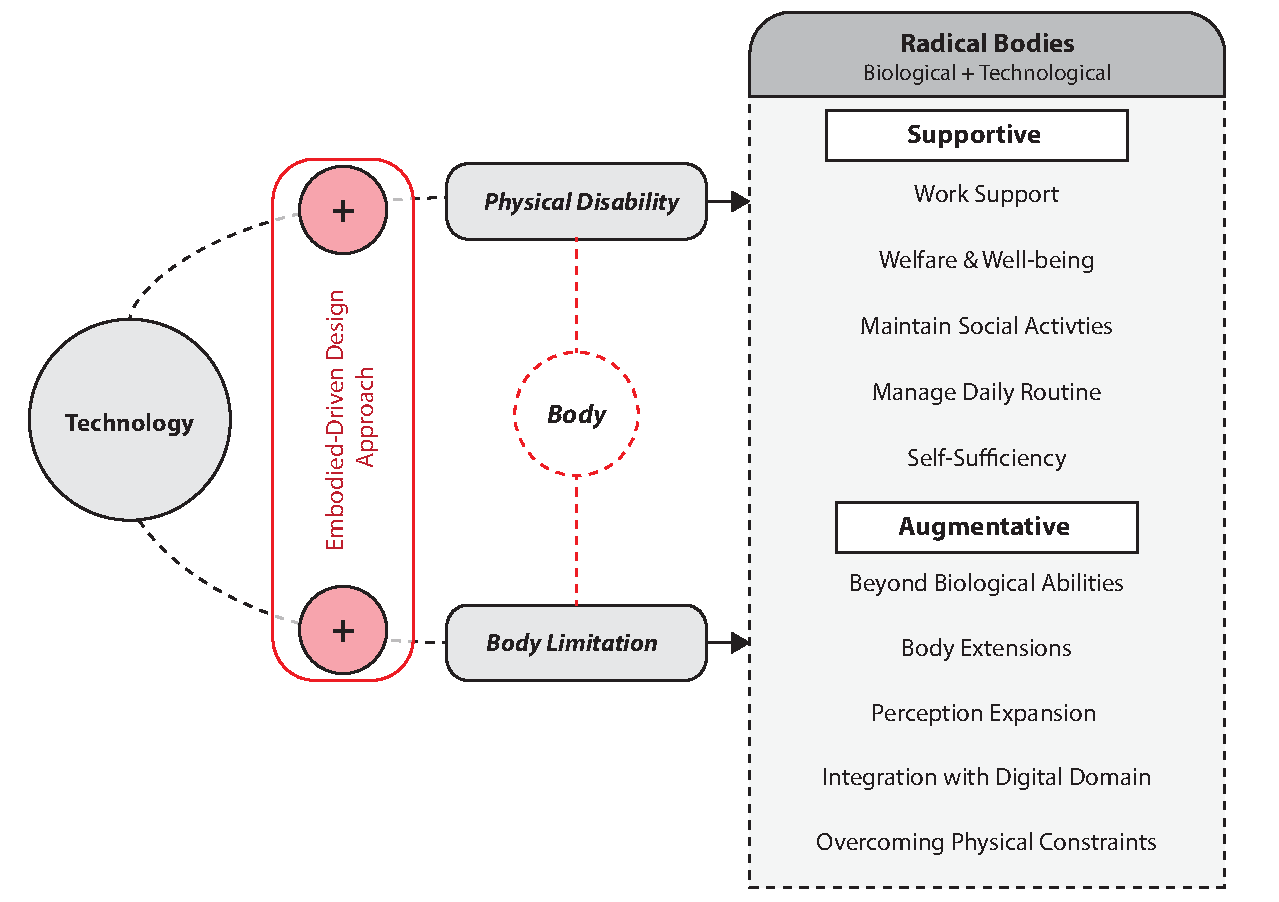
\includegraphics[width=1\linewidth]{figures/intro/RadicalBodies.pdf}
  \captionsetup{justification=centering}
  \caption{Radical Bodies, and the proposed Embodied-Driven Design (EDD) approach position.}
  \label{fig:intro-radicalbodies}
\end{figure}

Supportive tools help the physically disabled community to regain their lost functions and to assist them in engaging in their daily and social activities in an independent manner. According to the American Community Survey (ACS) \cite{disabilities2016}, an estimation of 12.6\% of the overall population in the United States suffers from a physical disability in 2015. The physical disability is varied as a hearing, vision, cognitive, ambulatory, self-care, and independent living. Also, the survey showed that the rates of disability increase with age. From the entire US population, for working class with ages of 18-64, the rate was 10.5\% (contributing to 51.1\% of the disabled community), while for elder people with ages of 65 and above the rate was 35.4\% (contributing to 41.2\% of the disabled community). The body inherited functions (non-cognitive) showed to be the highest factors to the disabilities. Tools for this category of users are described as Assistive and Adaptive technologies \cite{Tennessee2012standards}. Assistive Technology is any object or system that increase, maintain, or improve functional capabilities of individuals with disabilities (such as glasses, hearing aids, ...etc), while an Adaptive Technology is any object or system that is specifically designed for the purpose of increasing or maintaining the capabilities of people with disabilities and seldom to be used by non-disabled persons (such as wheelchairs, white cane, ...etc). That is, assistive technologies are the wider umbrella that adaptive technologies are a subset of. Adaptive tools usually require the disabled person to adapt to its new function and to train his cognitive skills to substitute his lost function ( a blind person needs to adapt to the limits and range of his white cane, as it will become his eyes). Thus it can be seen that our bodies (disabled or functional) have the capacity and plasticity to adapt to new representations of its functions. It is, however, the adaptation process is variant depending on the design and interaction with the substitution device or tool. If the user is required to maintain constant awareness toward the device used (through his various perceptual modalities), then the device is considered as a foreign object which does not function as an embodiment of his action.

Augmentative tools on the other hand leverage the functions of the human body, and allows to extend and expand beyond the inherited biological limitations. Augmentation technologies can be categorized into two classes: invasive and wearable (non-invasive). Each set of these two classes has its own merits as well as its disadvantages physically, socially, technically,..etc. As an example of the earliest trials on direct body implants of electronic devices other than for medical purposes, in 1998 professor Kevin Warwick implanted a radio transmitter into his left arm which communicates with computers to open doors whenever he approaches them. Interestingly, after nine days of using it, he reported the implant felt as being part of his body \cite{warwick2000cyborg}. Although this experiment can be seen as naive (a wearable device can serve the same purpose), but it was one of the initial trials of radical bodies changes, and has a future of transcending our bodies via the combination of biological and technological means. However, one of the major disadvantages of such augmentation is the high cost of replacement and upgrades both physical wise (need for a surgery, the risk of infections) and money wise (the cost for that surgery). Such augmentations are still immature technological wise, and widely unacceptable socially. The other set of augmentation, non-invasive type, had a better success at proving that our bodies can be altered safely and at rather low costs. This set has existed as far as the glasses were used to enhance poor vision. Neil Harbisson \cite{harbisson2012listen} used this type of wearable devices to overcome his color blindness by using a head-mounted camera which translates colors into sound frequency, and after adequate usage of it his perception adapted to this new perception. Current wearable technologies even provide a way to alternate our perception and realities. A \textbf{perceptual proxy} device, such as Virtual Reality (VR) Head Mounted Display (HMD), headphones, or tactile actuators, under certain conditions, can deliver sufficient information to sensory organs to convince the brain of the new reality. The idea of altering and augmenting our bodies has been a driving force for various technologies and media we use on a daily basis. This wave produced a constant hype towards human-centered technologies. A visible trend in empowering technologies can be seen by Gartner's review of emerging technologies hype cycle of the year 2016 \cite{hype2016gartner} in \Figure{fig:intro-hype}. Virtual Reality and Augmented Reality have already become mature enough for the end user's application due to the long history of trials and applications \cite{rheingold1991virtual}. However, Human Augmentation is still an emerging topic with high expectations for enhancing and empowering our bodies instead of just being a supportive hardware or for rehabilitation purposes. This topic is still in its infancy and requires further philosophical approaches and scientific experiments to evaluate its effectiveness. 

\begin{shaded}
\footnotesize
\centering
\textit{Radical Bodies are the result of the technological integration with our bodies, leveraging our physical constraints and enabling wider set of embodied functions.} 

\end{shaded}

\begin{figure}[t!]
  \centering
  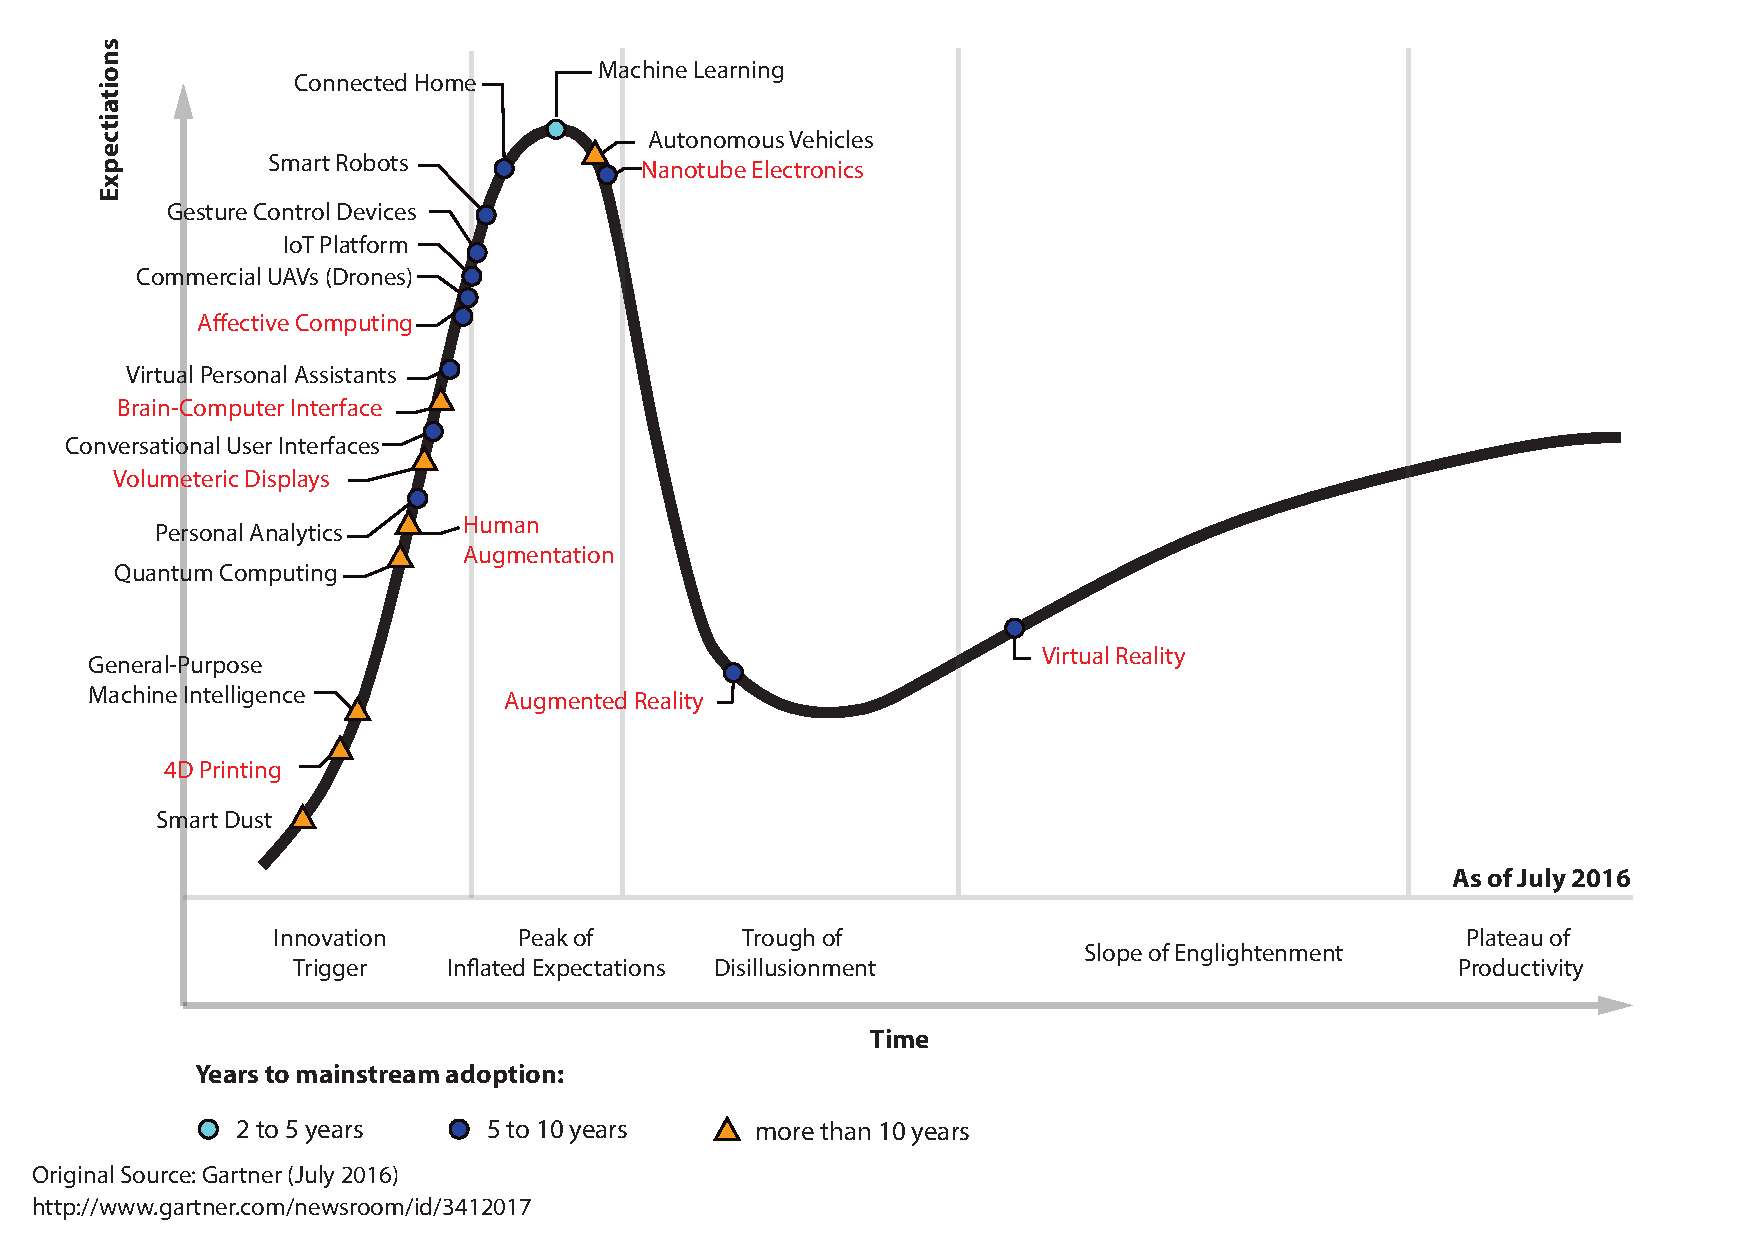
\includegraphics[width=0.9\linewidth]{figures/intro/gartner_hypecycle2016.pdf}
  \captionsetup{justification=centering}
  \caption[Gartner's Hype Cycle for Emerging Technologies 2016]{Expectations of human centered technologies. Gartner's Hype Cycle for Emerging Technologies 2016 (Modified from source for formatting purpose).}
  \label{fig:intro-hype}
\end{figure}

These tools and technological means have influenced radical changes to our perception and levitated our physical/mental abilities exponentially. The radical changes do not have to refer to the physical alteration of the human body (or mutations), but rather to how we act and communicate with the environment surrounding us. For example, today's advancement in the digital communication enabled us to overcome the spatial and temporal constraints. Internet-connected smartphones which are being used on a daily basis, have created radical changes in our social activities. A user communicating through it with a remote person is referred to be ``here'' and ``there'' at the same time. ``Here'' is where his physical body is located at which uses the smartphone to type and watch, while ``there'' is where a part of his cognition and awareness is actually at. Furthermore, virtual reality tools can carry the entire sense of presence and awareness into a totally different space or reality, in which the human body is no longer constrained by any physical limitations. The physical body is no longer defining the action, rather is being the medium between the internal intention and where the action is being performed. The more these technologies are integrated to our daily routine and appliances, the further the radical changes will be reflected on our bodies, and the more our biological bodies will be transparent in the process (mediums of actions). What if its possible to think of the body as being just a medium? Is possible to redefine this medium or ``rewire'' methodically? How to maintain this newly defined medium as being part of the body, or being the new body? In this thesis I address these questions by proposing the idea of ``Embodied-Driven Design (EDD)'', the use of body functions and modalities abstraction to allow us to redesign the functionality and the mapping of the body while maintaining the sense of ownership toward it.  \Figure{fig:intro-radicalbodies} shows the position of Embodied-Driven Design as an approach to establish a binding between our biological bodies and technologies in order to over come a physical disability or a limitation inherited within our bodies. EDD establishes an abstract modeling approach in order to reconfigure our bodies with an alternative representations, thus altering the embodied actions and cognition using mediated technology.

%To support this transition, or the integration between biological bodies and artificial means, a major research area ``Augmented Human'' has been established to leverage the human bodies capabilities using mediated tools.

%\subsection{The Hype of Human Augmentation}

\pagebreak
\section{\ProposalKeyword}% Metapresence

%\textit{\textbf{``Meta'': Abstraction} referring to a high level design approach.}

%\updatedtext


In this section, an overview of the thesis is described, the motivation and concept progression, along with the proposed approach addressing the thesis statement. 

\subsection{Thesis Statement}

In this thesis, I discuss the possibility to re-configure our bodies in a way that can alter our cognitive abilities or overcome our innate limitations and physical disabilities using mediated representations. With such re-configurations and alterations of our body schema, we can look at the use of the representations (for example technological tools) as being part of our bodies, embodied in a way we interact through them instead of using them. This sort of embodiment can establish a new form of interaction loop between our bodies and the environment (locally or in a different location), that our cognition is shifted into the active performance of intended actions instead of how we use the tools to achieve such actions. The relationship between body and action is mediated through embodied means of interactions and representations. This shift of perspective in using tools and technology would create an impact on how we perceive through and act within the environment in a way our bodies become actively part of it through our mediated and embodied actions. 

%Here I propose an Embodied-Driven Design approach for altering the body mapping, and focuses on the body transfer model in which it defines the relationship between the human body and the representation used. This approach is concerned with the flow of the body actions and sensory feedback, and it defines the interaction loop of the body model with its representation(s). Both the transfer model and the representation are the actual realization of the intended body schema model.

%Using this proposed approach, it is possible to adapt to new body forms which are considered driven from our embodied behaviours. 



\subsection{Motivation \& Approach}

The capability of remapping our exteroceptive modalities (visual, auditory, tactile, taste, and smell), and proprioceptive modalities such as body and joints posture with an alternative body representation can help to levitate the upper bounds of our physical limits. For example, for a true ubiquitous presence a person should be capable of receiving inputs from multiple locations simultaneously, thus we can say this person is ubiquitous as being in everywhere. His body and sensory modalities are not ``physically'' there, but his perception of these modalities is linked to them, and body sensory flow has became altered and remapped. Other topics can also be achieved, such as expanding the localization of body parts from being tightly coupled in one location (on the body) into being loosely coupled and distributed in multiple locations. Adding to that, body representation does not have to be tangible as long as it serves the application intended to, for example when the body is needed to represent the visual appearance of the user or the state the user is at, then it's sufficient to use a non-physical representation for that purpose. In these terms, the concept of body stretches from a tight physical representation which its parts are coupled spatially and tangibly, into loose physical/virtual representations that can be restructured and remapped. This expansion would provide new forms of awareness alterations and perception enhancements. Indeed there are issues that might arise when new forms of perceptual augmentation occur which we are not adapted to, such as perception overload (when several information sources are provided into the same perceptual modality, such as eyes or ears), or non-intuitive interaction is being used (not correlated with body motion, and requires training to learn it). 

In this thesis, I argue that the human body schema can be altered and adapt to new forms of body structures as long as the actions mapped between the body and its new representation are correlated. \ProposalKeyword conceptualizes the idea of using digital media and mediated technologies to alter human body properties on a high and abstract level, achieving new ways to transcend our perception and body capabilities. This approach addresses both local and remote body mapping, expanding the human spatial reach and reducing the physical constraints. \ProposalKeyword derives from the school of philosophical thought named as ``phenomenology'', which is concerned with how we perceive, experience, and act in the environment surrounding us using our body. Further details regarding the philosophical background of this research will be discussed in \Chapter{ch:related}. 

\subsection{Concept Development}

The human body is the interface of the mind, the medium to the tangible world and the embodiment of our thoughts. Its where the action is performed at and its the bridge which connects our world too, what we may say our self. My research and background in Telexistence area had inspired me to focus more on the possibilities to use mediated technology to expand our body instead of just replicating it. How to create a model of the human body that enables us to extend, enhance, and modulate our embodied functions was and still the driving force of \ProposalKeyword. I believe that in order to come up with such a model, an abstraction of the human body is needed that provides a systematic approach to embodied modeling.

This thesis investigates toward an abstraction model of the human body that enables us to redefine the actions and affordabilities which our cognition can represent. Our bodies constitute physical limitations, while the inner mental model of the body is far more adaptable to variations and reconfigurations. This work shows the possibility to rewire (or reprogram) the body in order to overcome an existing physical disability or to leverage the capacity of human body perceptual \& postural limitations. These arguments are supported by philosophical background research and empirical studies that build up the concept of \ProposalKeyword.

The idea behind \ProposalKeyword was developed across several projects and iterations which helped me to generalize the idea of meta-modeling, and the design of body schema transfer systems. Along these iterations, four different meta-modeling approaches were developed and used to address body limitations and physical disabilities. These meta-modeling approaches were used in five projects. These iterations along with the projects that involved in each of them are illustrated in \Figure{fig:intro-progression} with the corresponding projects that address. 

The first design iteration \textit{Direct Body Transfer} was initiated based on my involvement in Telexistence area of research since 2013. This approach develops the concept of mapping our body's functions and modalities directly into a corresponding representation without the need of alteration or modifications. Such mapping pattern is useful to transfer body parts directly from one location to another. Telexistence type of systems uses such pattern to copy user's body motion into a remotely connected avatar system, and replicate the feedback back to user's body. ``Telexistence based Surveillance System'' project in the period of 2014-2016 (\Section{sec:eval-txSys}) mainly uses this design approach to overcome body spatial limitations.

%This approach basically contributes at the type of systems that overcomes spatial constraints in teleoperation applications. My involvement in ``Telexistence based Survellance System'' project in the period of 2014-2016 (\Section{sec:impact-txSys}) developed the necessary elements for providing direct and real-time body transfer systems. This approach has been incorporated as a basic building block for direct body transfer meta-modeling. 

\begin{figure}[t!]
  \centering
%	  \centerline{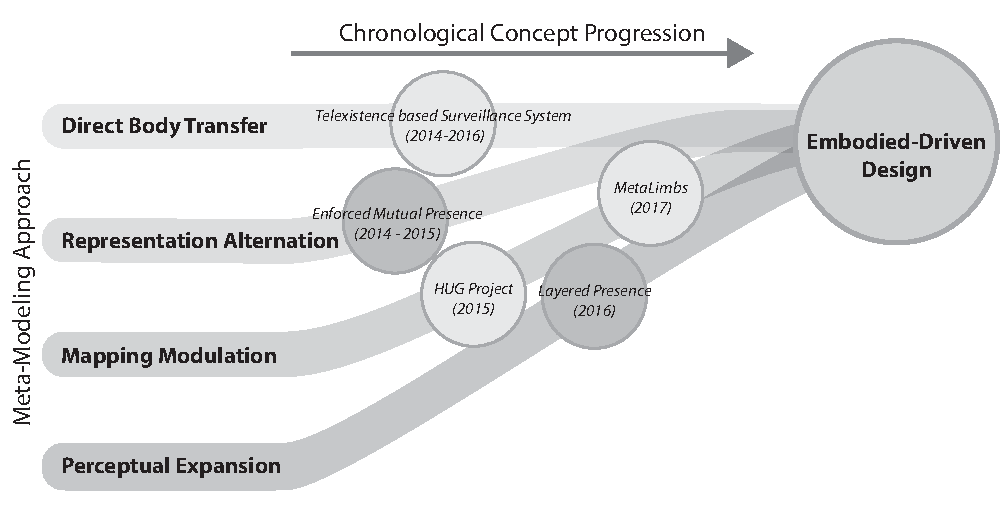
\includegraphics[width=1.2\linewidth]{figures/intro/ConceptProgression.pdf}}
	  \centerline{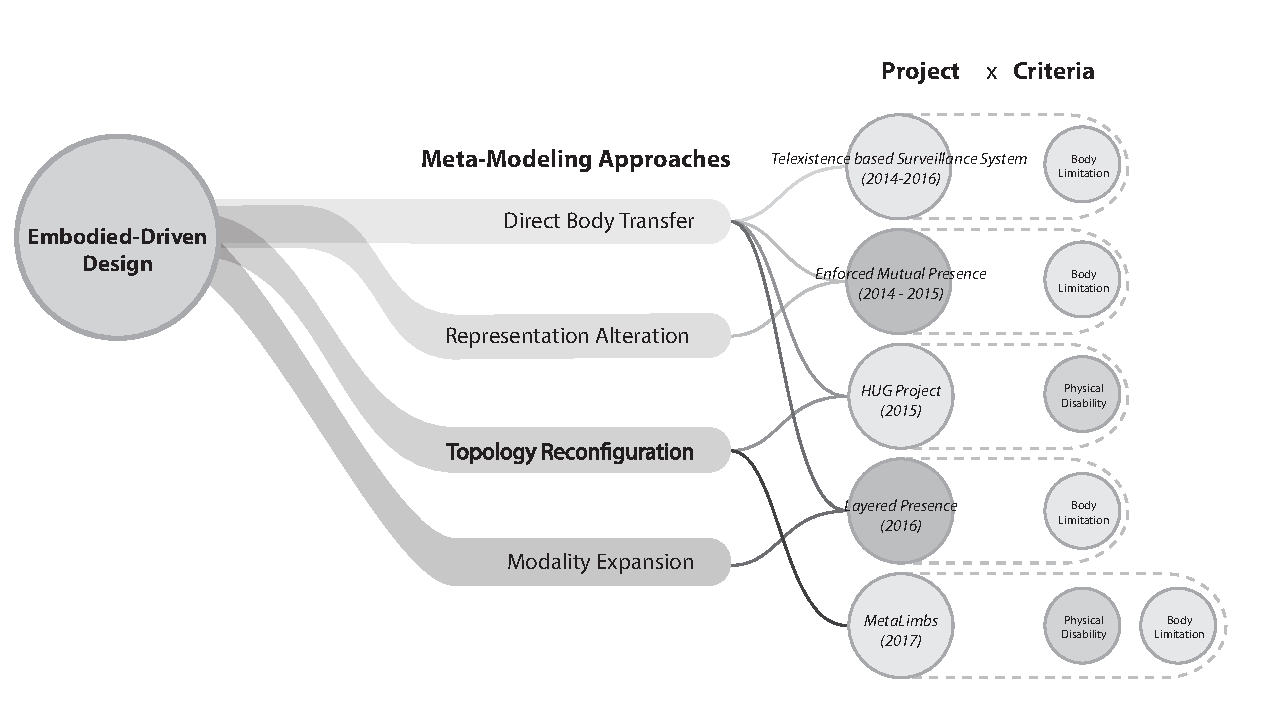
\includegraphics[width=1.2\linewidth]{figures/intro/MetaModelingOverview.pdf}}
  \captionsetup{justification=centering}
  \caption{The use of Embodied-Driven Design Meta-Modeling approaches to address five projects, highlights the need of such design approach to resolve body limitations and disabilities.}
  \label{fig:intro-progression}
\end{figure}

The second design iteration \textit{Representation Alteration} aims to overcome the physical limits constituted by our bodies. It combines a hybrid approach for altering the representation of our bodies using virtual and physical means. Thus the body is mediated through tangible and non-tangible representation overcoming certain physical limitations. ``Enforced Mutual Presence'' achieved in 2014-2015 (\Section{sec:eval-enforced}), explores the use of virtual representation along a physically teleoperated system to achieve a full sense of body presence despite the fact the system does not have a full physical body. Virtual hands substitute user's arms were projected locally and remotely at the teleoperated system. This substitution not only helped at providing the full awareness of the body, but also the use of non-physical hands helped to overcome the tangible constraints of arm's length limits. Thus the operator is capable to stretch his body across spatial space. With such alternative body representations, it is possible to design new body forms that overcome our bodies' physical limits (such as extending arm reach and pointing for mobility impaired people).

%This project helped at defining a meta-model for representation alteration, that is the use of a combination representations for the body. With such alternative body representations, it would become possible to design brand new radical forms which our physical bodies can not achieve.

%The use of direct body mapping means that the representation side is required to have same functions which the human body can link and map into, such as physical arms, hands, eyes, ...etc. However, in situations that the representation does not matches human body properties and topology, then 

%To overcome such a requirement, the second iteration was aimed to solve the physical body constraints by using hybrid body representations. Enforced Mutual Presence 2014-2015 (\Section{sec:eval-RepAlt}) explored the use of virtual contents along a physically teleoperated system to achieve full sense of body presence despite the fact the system does not have full physical body. The approach used is to use virtual hands driven from the user's body which are projected locally and remotely at the teleoperated system. This not only helped at providing the full awareness of the body, but also the use of non-physical hands visuals helped to overcome the tangible constraints of arms length limits. Thus the operator is capable to stretch the body across the spatial space. This project helped at defining a meta-model for representation alteration, that is the use of a combination representations for the body. With such alternative body representations, it would become possible to design brand new radical forms which our physical bodies can not achieve.

The third design iteration \textit{Topology Reconfiguration} explored the plasticity of human body operation mapping, mainly the postural mapping. Two projects helped in formulating this design approach: the first is ``HUG Project'' in 2015 (\Section{sec:eval-hug}) that used eye gaze input to control the head rotation of a remote system supporting a physically disabled person to operate it. The second project is ``MetaLimbs'' in 2017 (\Section{sec:eval-metalimbs}) that explored remapping body legs with artificial arms mounted on user body, thus expanding the number of independent arms. Both projects showed the immediate adaptation the body can achieve to a different mapping schema. This iteration established the design of body postural topology that is used as one of the foundations of this approach.

Last design approach explored is \textit{Modality Expansion} that addresses the possibility to expand the perceptual modalities of our body and the capacity to remap our sensory and postural topology to multiple representations simultaneously. ``Layered Presence'' in 2016 (\Section{sec:eval-layeredpresence}) studied this body schema and proposed a modeling approach to achieve such expanded spatial awareness. This project helped to shape the perceptual modalities mapping and an interaction model which helps in developing this approach.

These four iterations motivated the design of a meta-modeling approach for human body schema, and defined the foundations of the proposed modeling framework. \ProposalKeyword and its realization as a framework are aimed to assist designers and researchers in this field to prototype and deploy new forms of body schema.


%This work proposes a novel design approach for altering human perception mapping with remote avatar surrogates to achieve what is called ``\ProposalKeyword'' based on \textbf{Loosely-Coupled Modality} (LCM) design pattern, and using \textbf{Embodied-Driven Design} (EDD). Using this design concept, the perceptual representation combines both physical and virtual tools to define to reconstruct the relationship between our sensory organs and the corresponding inputs, and same wise for actuating organs. \Figure{fig:intro-evolvement} shows the differentiation between Telepresence and Telexistence in terms of design perspective. Metapresence covers the concepts in Telexistence, and adds an embodied driven design approach using meta prototyping tools. Further details follows in Chapter 3 about Metapresence design approach.

%      Further details follows in Section \ref{sec.EDD}.





%%%%%%%%%%%%%%%%%%%%%%%%%%%%%%%%%%%%%%%%%%%%%%%%%%%%%%%%%%%%%%%%%%%%%%%%%%%%%%%%%%%%%%%
\subsection{Research \& Design Topics:}


\Table{intro:research-topics} summarizes an overview of the topics that constructs the concept of \ProposalKeyword. Research and design topics addressed in this thesis outline body schema modeling approach.

The first part addressed is focused on the design approach for \ProposalKeyword and is discussed in \Chapter{ch:concept}. A framework is developed based on a systematic model of human body schema in which its possible to remap and restructure it hierarchically. It outlines the methodology to form a meta-modeling approach that realizes the proposed concept. EDD is constructed and designed based on the following topics:

\begin{enumerate}[label=T\arabic*.]
 \setlength\itemsep{0em}

\item \textbf{Loosely-Coupled Modalities (LCM):}

Possibility to decouple body modalities into a set of ``input/output channels'', and to re-couple them. The loosely representation helps to break the coupling of the physical modalities and constraints, and thus allows to achieve a higher level of mapping of the human body to its representation(s). LCM defines two topologies for the human body: Postural and Sensory. These topologies serve as generalization and abstraction for the postural modalities of the body (connection between the various body joints), and the sensory modalities. Further details are discussed in \Section{sec:concept-LCM}.

\item \textbf{Body Schema Meta-Modeling:}

Ability to remap our bodies modalities into new body schema. This topic argues that our body structure can be reconfigured or reprogrammed. The meta-models define the structure of the sensory and postural channels mapping between the human body and the corresponding representation(s)' modalities. In these models, transfer blocks are used to characterize the function and data flow between the modalities used. Further details are discussed in \Section{sec:concept-bodyschema}.

\item \textbf{Meta-Modeling Approaches:}
Four meta-modeling approaches are proposed that summarizes the general usability methods of EDD within this thesis, and which can be generalized for applications beyond what is discussed. The purpose of these approaches is to facilitate the design process, and to highlight how to address body limitations and disabilities using meta-modeling. Further details are discussed in \Section{sec:concept-metalmodel}.

\end{enumerate}


\begin{table}[t!]
\scriptsize
\centerline{
\begin{tabular}{lll}
\toprule
  \textbf{}    & \textbf{Category} & \textbf{Reference} \\ 
\midrule
\textbf{Topic} &    \textbf{Embodied-Driven Design}       &   \Chapter{ch:concept}   \\
\textbf{T1.} & Loosely-Coupled Modalities: Recon-structure body schema based on a hierarchical topology  &       \Section{sec:concept-LCM}     \\
\rowcolor[gray]{.9} 
\textbf{T2.} & Body Schema Meta-modeling: Abstraction of body modalities interaction and mapping  &   \Section{sec:concept-bodyschema}    \\ 
\textbf{T3.} & Meta-Modeling Approaches: Four design patterns for body schema editing &   \Section{sec:concept-metalmodel}    \\ 
\midrule
\textbf{Project} &    \textbf{Meta-Modeling Evaluation}        &  \Chapter{ch:eval}   \\
\textbf{P1.} & Telexistence base Surveillance System: Addressing spatial limitations & \Section{sec:eval-txSys}              \\
\rowcolor[gray]{.9} 
\textbf{P2.} &  Enforced Mutual Presence: Addressing body physical limitations & \Section{sec:eval-enforced}  \\ 
\textbf{P3.} &  HUG Project: Addressing body plasticity to overcome physical disability   &  \Section{sec:eval-hug}                \\ 
\rowcolor[gray]{.9} 
\textbf{P4.} &  Layered Presence: Addressing perceptual plasticity  & \Section{sec:eval-layeredpresence}  \\ 
\textbf{P5.} &  MetaLimbs: Addressing body plasticity and limbs limitations       &  \Section{sec:eval-metalimbs}                \\ 
\bottomrule
\end{tabular}
}

  \captionsetup{justification=centering}
\caption{Topics and projects addressed in this thesis to realize \ProposalKeyword. }
\label{intro:research-topics}
\end{table}



The second part of this thesis in \Chapter{ch:eval}, evaluates meta-modeling approaches through five different scenarios addressing human body limitations and/or physical disabilities. An overview of the main points addressed within these projects as follows:

\begin{enumerate}
 \setlength\itemsep{0em}
\item Spatial limitations: Expanding body spatial accessibility and awareness through mediated representations, which is mainly addressed through P1.``Telexistence base Surveillance System'' in \Section{sec:eval-txSys}.

\item Body physical limitations and disabilities: Possibility to use different body representation to overcome physical constraints, addressed through P2.``Enforced Mutual Presence'' in \Section{sec:eval-enforced}, P3.``HUG Project'' in \Section{sec:eval-hug},and P5.``MetaLimbs'' in \Section{sec:eval-metalimbs}.

\item Perceptual plasticity: Use of EDD to alter body modalities to expand the amount of perceptual feedback. P4.``Layered Presence'' in \Section{sec:eval-layeredpresence} illustrates visual perception plasticity into multiple remote locations.

\end{enumerate}

%\Figure{fig:intro-meta} highlights the differentiation between Telepresence and Telexistence design approaches, and highlights Metapresnce conceptual design.


%%%%%%%%%%%%%%%%%%%%%%%%%%%%%%%%%%%%%%%%%%%%%%%%%%%%%%%%%%%%%%%%%%%%%%%%%%%%%%%%%%%%%%%

\subsection{Summary of Contribution} 

The main contributions of this thesis can be categorized as follow:
\begin{itemize}

\item Conceptual Contribution: 

This thesis provides the building blocks for expanding and enriching the body augmentation area of research by connecting the theoretical studies and various questions in the philosophy of body ownership and metacognition with systematic methods for testing these theories. By providing a framework for body schema design and modalities alteration, it is possible to design and evaluate various models of body schema with an experience-oriented approach.
%evaluate and measure the degree of cognition and perception human can be aware of. 

\item Design and Implementation:

This thesis presents the design strategy of body schema meta-modeling based on four modeling categories: direct body transfer, representation alteration, topology reconfiguration, and modality expansion. These meta-models summarize the general design approaches which the body schema can be designed through. Each of these categories is addressed separately.

\item Social and Industrial Contributions:

During the course of this thesis, two projects in which the Embodied Driven Design (EDD) framework was used into. The first is ``HUG project'' in which EDD used as a social contribution, and ``Telexistence based Surveillance System'' as an industrial contribution.

\item Technical Contribution: 

Along the development of this work, various system optimization and technical details that assist the developers in telepresence/telexistence related applications were described in this thesis, such as \textit{Foveated Streaming}. These details are further discussed in \Chapter{ch:impl}.

\item Physical Embodiment Toolkit: 

As an outcome of this work, an embodiment toolkit has been designed and implemented. This toolkit provides essential functions for remote presence applications, and its functions have been integrated into the EDD framework as a set of representation modalities which can be accessed and mapped with user's body. This toolkit allows designers to use rapid prototyping and testing of their ideas along with the meta-editor.

\end{itemize}


\pagebreak
\section{Thesis Outline}

This research builds on the findings related to human body plasticity found in the areas of philosophy of body and perception, cognition science, and body augmentation. Also, it introduces the idea of \ProposalKeyword: altering body schema and sense of presence using a systematic and at a meta-level design. This thesis highlights the idea of digitized modalities -converting the biological/analog sensory and motor modalities into a digital representation- in order to overcome the inherited physical constraints and limitations. 
%By using the idea of digitized modalities, its possible to modify the perceptual information in a mediated environment in order to augment the human body. And with the ability to map and restructure body's functions into different schematics, it is possible to compensate a disabled function of the body by deriving its functionality from a different modalities, e.g. mapping a functioning limb into a disabled one.

%\end{itemize}


%\subsection{Meta-Modeling of Human Body}
%\pagebreak
%\section{Thesis Outline}

\subsection{Organization}

The core of this thesis is divided mainly into four parts and seven chapters organized as follows:

\begin{itemize}
\item \textbf{\Part{pt:I}: Foundations \& Philosophy}
\begin{itemize}[label={},leftmargin=*]
\item \textbf{\Chapter{ch:intro}.} provided the motivation behind this work, and briefly introduced the proposed concept: Embodied Driven Design.

\item \textbf{\Chapter{ch:related}.} explores the literature and philosophical background which Embodied-Driven Design is established on top of. Discusses topics related to Embodiment and Cognition that are regarded as the fundamentals of this research, and in which the idea of Embodied-Driven Design is placed within. It also provides several related work in human augmentation, presence alteration, and body representation which this research concept derives from, highlighting the contributions of this thesis.
\end{itemize}

\item \textbf{\Part{pt:II}: Embodied-Driven Design}
\begin{itemize}[label={},leftmargin=*]
\item \textbf{\Chapter{ch:concept}.} discusses in further details the proposed concept of embodiment design and the overall design considerations for an EDD framework, including the concept of loosely-coupled representation for human body. Four types of meta-modeling categories are described which summarize the design approaches of EDD: Direct body transfer, Representation alteration, Topology reconfiguration, and Modality expansion.

\item \textbf{\Chapter{ch:impl}.} provides the implementation process of EDD framework and meta-modeling editor environment, and describes in details the various building blocks for modeling body schema. The development of a physical toolkit is also discussed along EDD framework for general purpose presence embodiment.

\item \textbf{\Chapter{ch:eval}.} discusses five different projects and use-cases that highlights the role of EDD meta-modeling to resolve body limitations and physical disabilities. These study cases show the possibilities to modify our body schema to achieve new cognitive capabilities, such as expanding visual awareness and altering body limbs. 

\end{itemize}

\item \textbf{\Part{pt:IV}: Future Direction \& Conclusion}
\begin{itemize}[label={},leftmargin=*]
\item \textbf{\Chapter{ch:conc}.} concludes with a summary and reflections of this work, main contributions and outcomes, limitations, and finally presents an outlook for this research future direction. %, the limitations, and future direction to expand the topic of embodiment design and Metapresence applications.

\end{itemize}
\end{itemize}

\pagebreak
\section{Glossary}

The following keywords are described in the context of this thesis:

\begin{itemize}
\item \textbf{Agency}

Motor skill control, including the subjective experience of control, intention, sensory-motor selection and the conscious experience of will. Further details about the topic \cite{roessler2003agency}.

\item \textbf{Body Schema}

The mental model or self-image of the body, a subjective experience obtained through the cycle of operation and sensory feedback to create the global structure of one's perceived body.

\item \textbf{Embodiment}

The subjective experience of 'having and using' a body which interacts with the external surroundings, and reflects the inner intentions in correlation with cross-modal perception. The act of embodiment alters the mental image of body schema.

\item \textbf{Loosely-Coupled Modalities}

The possibility to decouple body modalities into a set of ``input/output channels'', and to re-couple them. The loosely representations help to break the rigid constraints of the physical modalities, and map body modalities separately.

\item \textbf{Meta-Modeling}

The process of defining an abstract model for the relationships between the various body modalities provided with an artificial representation's modalities.

\item \textbf{Modality}

In this thesis, a modality refers to a functionality derived from the human body or an artificial representation. The functionality can be described as an input if its related to the sensory feedback of the body, and an output if its related to an action can be performed by the body, such as joints motion.

\item \textbf{Ownership}

A reflected experience of identification a body as being owned by one's self (phenomenally experienced as 'mine-ness').

\item \textbf{Perceptual Proxy}

A device used to deliver/receive information to sensory/from actuating organs to induce a new sense of reality or to capture the structure of the body. Such as virtual reality equipment, haptic feedback interfaces, postural tracking devices.

\item \textbf{Radical Bodies}

The concept proposed in this thesis reflecting the radical changes of technology progression on human bodies in terms of interaction and perception within an individual or social contexts.

\item \textbf{Representation}

In this thesis, representation refers to the physical or virtual form of the modalities which can act as an extension or replacement of certain human body modalities. % (the relationship is defined by the meta-model)

\end{itemize}


%\footnotesize
%\bibliographystyle{dependencies/acm-sigchi}
%\bibliography{y-bibilography}   %20 pages
		
\chapter{Literature Review}
\label{ch:related}
\markboth{Literature Review}{}


\begin{flushright}
\textit{
``Before paper, wires, and silicon, the primordial communication medium is the body. At the
center of all communication rests the body, the fleshy gateway to the mind''}
\par\hfill\textsc{Frank Biocca, The Cyborg's Dilemma 1997}


\end{flushright}
\vspace{15pt}

Embodied-Driven Design approach has been proposed based on the work and philosophy done in embodiment area of research, and derives mainly from Presence Augmentation and alteration, Body Representation, and related disciplines. This chapter explores theories in philosophy regarding embodiment and body schema theories, also discusses related work that focuses on altering body interaction with the environment for augmentation or substitution purposes.
%EDD modeling framework proposed in this research is derived from Meta-Modeling design. As described in the previous chapter, the idea of Metapresence is tightly related to the work and philosophy done in the embodiment area of research. In this chapter, further work done by recent research related to human perception augmentation and enhancement is discussed here. %Based on that, its possible to place Metapresence within this research paradigm, and to show the necessity of this proposed idea.


%%%%%%%%%%%%%%%%%%%%%%%%%%%%%%%%%%%%%%%%%%%%%%%%%%%%%%%%%%%%%%%%%%%%%%%%%%%%%%%%%%%%%%%%%%%%%%%%
\section{Body and Embodiment}

\begin{flushleft}
\textit{
``I think, therefore I am''  }\textsc{René Descartes}
\end{flushleft}

%``I think, therefore I am'' René Descartes
% Thinking and Cognition   <---> Embodiment and Existence
%How the body shapes the way we think: Rolf Pfeifer at TEDxZurich
%How the brain is embedded into the physical system that embodies it
%\cite{pfeifer2006body}
Several theories of mind and body have been formulated on the idea that our bodies and thinking are two separate worlds. \textit{Computationalism} theories that were derived from this perspective of mind, has been widely adopted as in various fields of robotic design to mimic the sensing behavior of the body (the one that interacts with the physical domain), and the processing behavior of the mind (the one which uses algorithmic computations). These perspectives isolate the role of the body in shaping cognition, and thus they disembody the brain from the body. 


\begin{figure}[t!]
  \centering
    \centerline{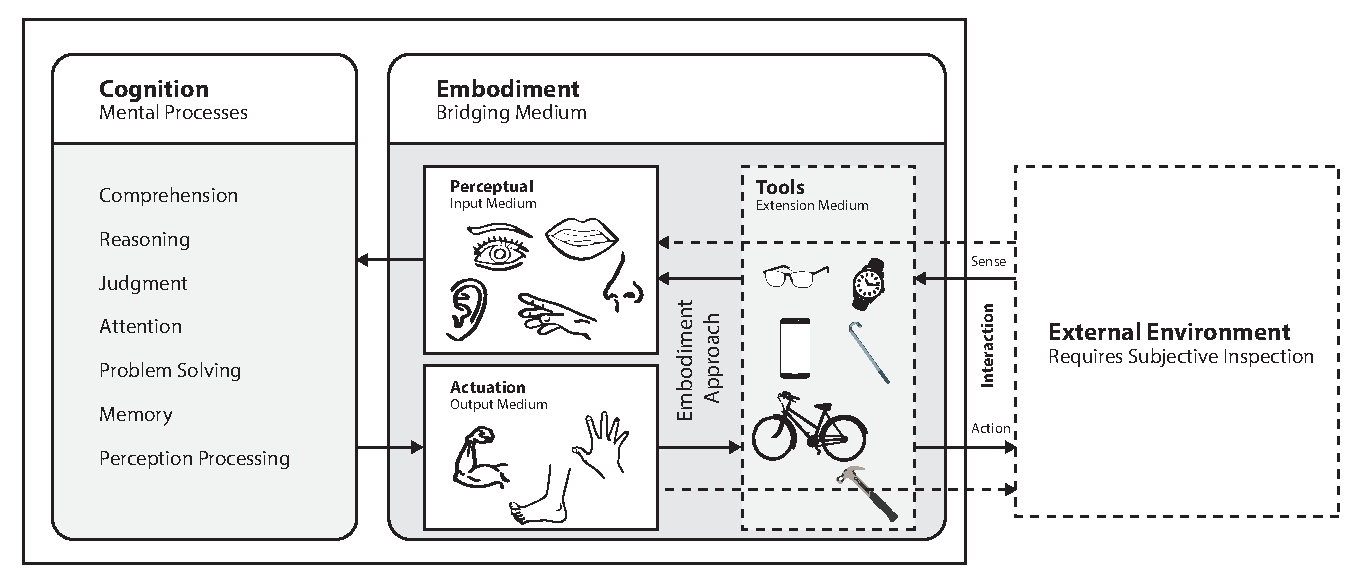
\includegraphics[width=1.3\linewidth]{figures/intro/Embodied-Cognition.pdf}}
  \captionsetup{justification=centering}
  \caption{Embodiment of tools to extend our cognition and actions into the external environment.}
  \label{fig:intro-embodiment}
\end{figure}

In philosophy and literature, embodiment has taken various definitions and concepts. MacLachlan \cite{maclachlan2004embodiment} has defined Embodiment as: \textit{the identification of an abstract idea with a physical entity}, however this base definition is rather too broad and the concept of the \textit{idea} can be self, emotion, intelligence, ...etc. Whenever this \textit{idea} is represented in a tangible matter, it can be declared as being \textit{incarnated}. Although Embodiment falls into different categories (psychology, sociology, computer science, ...etc), however, all are mainly centered around the human being, the entity with cognition and awareness. In literature and philosophy, Embodiment focuses on the relationship between our bodies and the environment surrounding it, how do we conceive information, and links to them inside-out/outside-in our mental model. Furthermore, how human cognition is shaped based on what we perceive, that is, we are what we perceive(d) and experience(d). As Shapiro describes this theme of embodiment as Conceptualization \cite{shapiro2010embodied}, our body structure defines our comprehension of surrounding world. Thus it can be viewed that human body is the interface of the mind, the channels which communicate with the outside world, and as the tangible representation of an internal idea, a thought, or an opinion when being expressed in a physical form. The expression can be a form of an act (moving a muscle group), verbal sounds (speaking), or a mediated action (through a tool, an interface, or written symbols). Likewise, perception is done through one of the five sensory organs we have: visual, auditory, tactile, smell, and taste organs. 


%describe the importance of cognitive science and embodiment here
%The standard cognitive science focuses on the idea that human perception and reasoning can be regarded as a computational model, and uses rules and symbols 

\begin{quote}
``The body is our general means of having a world. Sometimes it restricts itself to gestures necessary for conservation of life, and correlatively it posits a biological world around us. Sometimes, playing upon these first gestures and passing from their literal to their figurative sense, it brings forth a new core of significance through them - this is the case of new motor habits, such as dance.'' (Maurice Merleau-Ponty Phenomenology of Perception 1945 p.147)
\end{quote}

An ecological theory of perception was presented by Gibson \cite{gibson1966senses} which suggests that brain resonates to information presented in the environment surrounding it. That is, a structured information stimulating the sensory organs, and a brain resonating to these sensory inputs. Adding to that, Gibson's view of information acquisition insists on the fact that sensory organs should hunt for them by active involvement in the environment. 

\begin{quote}
``The perceptual systems, as it turns out, correspond to the organs of active attention with which organism is equipped... Head movements, ear movements, hand movements, nose and mouth movements, and eye movements are part and parcel of the perceptual systems they serve. These adjustments constitute modes of attention... They serve to explore the information available in sound, mechanical contact, chemical contact, and light.'' (Gibson 1966 p.58)
\end{quote}

Modern philosophers looked into the expansion of our mind using the tools that we use, representing an extension of our bodies \cite{shapiro2010embodied, malafouris2013things}. Describing the body extension phenomenon we experience when using tools \Figure{fig:intro-embodiment}. As an example, visually impaired and blind people commonly use a white cane to extend their tactile perception, and to feel objects surrounding them. Another example for entire body expansion is a bus driver, what distinguishes a professional driver from a novice one is the capability to have complete awareness of the bus he is driving, and feel it as being an extension of his body. To use the mirrors as an extension of his visual sense, driving wheel as an expansion of his motor cortex functions, and the horn as a new way of communication. The process of adapting to the tool also shape our embodiment into it, until we learn how to use it without thinking of the procedure which its operated with, as an example, when driving a bicycle \Figure{fig:intro-bicycle} we do not think of the handlebar while steering (embodied), actually when we think of how we are using it then we might lose balance and fall off (became disembodied). 


\begin{figure}[htpb]
  \centering
    \centerline{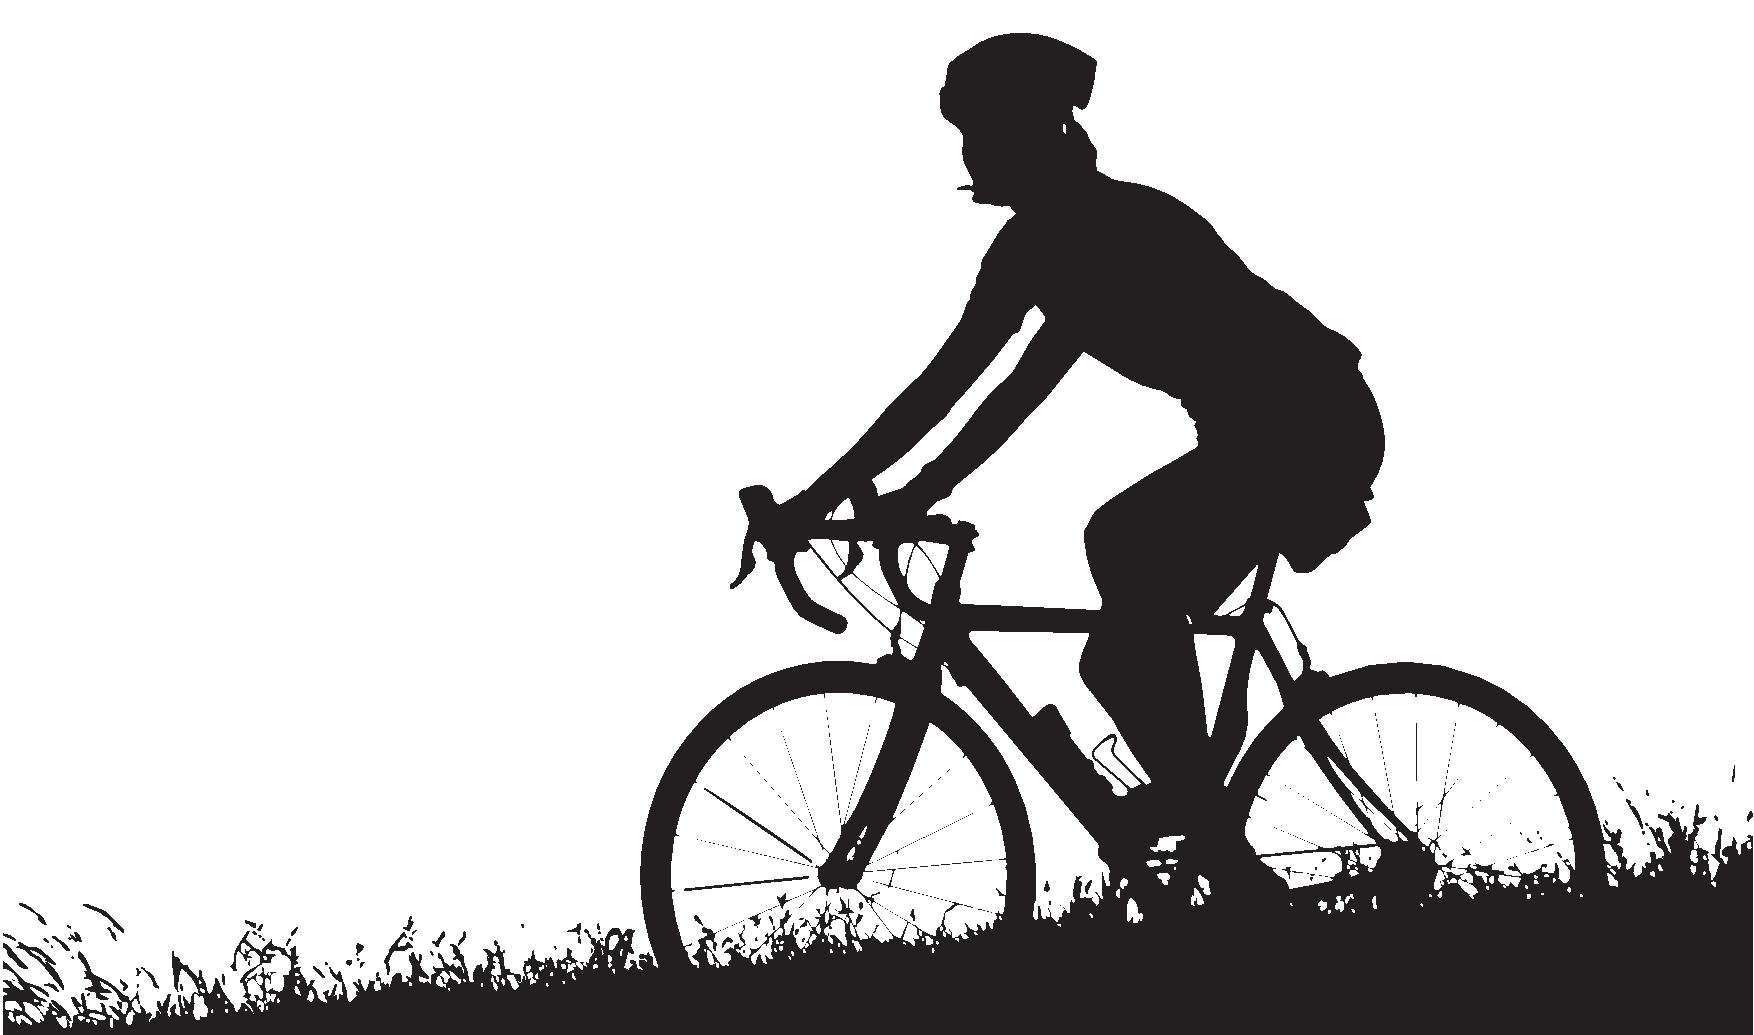
\includegraphics[width=0.8\linewidth]{figures/intro/Bicycle.pdf}}
  \captionsetup{justification=centering}
  \caption{The use of bicycle morph our bodies, and embodies our actions through it.}
  \label{fig:intro-bicycle}
\end{figure}

Building on top of these principles of embodiment and cognition, psychologists and researchers in this field \cite{marcel1995body,gallagher2006body,pfeifer2006body,blanke2009full} began to formulate a better understanding of the body and its connection with our comprehensions of self and environment surrounding us. The cycle of interactions as input and outputs using our available modalities with the external world helps to shape a schema of our body with a mental model of it. 


\subsection{Embodied Self}

As has been discussed before, the type of representation used to reflect the inner cognitive thoughts or the medium of interaction plays an important role in communicating with the external world. The representation itself has attributes and functions that enable our cognitive functions to use and bridge with the outside world. These attributes define the level of interaction and awareness in the external environment.

In teleoperated environments, commonly operator's body is represented by a robotic form that focuses on the required operational purpose \cite{tsui2011exploring}, in which the considerations for designing the slave system is driven from the requirement of the scenario it will be used for. The design of the slave system reflects the control mechanism and the type of behavior the operator should follow to drive and operate the slave body, for example, to use a joystick to control the direction or a data glove to match slave manipulator position with hand's posture. For social and communication type of scenarios, the robotic representation is not always a necessity to be considered in the design of the system. For example, in mutual body representation, a visual representation is sufficient to transfer the state of the person located remotely \cite{ishii1992clearboard}, or for a group of people sharing the same space and collaborating remotely \cite{kunz2010collaboard} in which its possible to transfer important social aspects of communication such as eye gaze and hands gestures. Hybrid representations which both tangible and imagery representation to solve the body and social aspects as well as the physicality to manipulate remote objects were proposed. Physical Telepresence \cite{leithinger2014physical} or as commonly known as inFORM \cite{follmer2013inform} uses shape displays for interaction mediation. This type of body representation is mediating the action of the body rather than the actual spatial and physical state of it. From the user point of view, these systems do not provide a full sense of immersion, but rather as being looking through a window or medium which they perform their actions within rather than being the medium.

Virtual representation of the body has enabled to overcome the physical constraints of the representation. Ogawa et al. \cite{ogawa2012reachable,ogawa2016metamorphosis} proposed a user interface which extends hands interaction by deforming the visual feedback of user's arm, such as extending its length to reach far objects. Asai et al. \cite{asai2016extendedhand} used this type of interaction for people with a mobility impairment to easily point to physically far surfaces. The virtual representation has also enabled social researchers to investigate the effect of changing body skin color or race to a different one to decrease the racial bias against dark-skinned people \cite{peck2013putting,rosenberg2013virtual}. The study highlights the importance of multisensory correlations to induce the illusion of body ownership toward the virtual body, which relates to the level of embodiment the participant's experience. Within the same context, \cite{maister2015changing} showed that experiencing a body with superpowers (as being a superhero in sci-fi) to fly in a virtual environment based on embodied actions, like acting as Superman to fly, would lead the participants to engage in a pro-social activity to help others in need after finishing the experience. Further investigations on reproducing the illusion of virtual body ownership for non-humanoid creatures has been studied in \cite{lugrin2015anthropomorphism}. Probably the virtual bodies are the true alchemy of embodiment.


%%%%%%%%%%%%%%%%%%%%%%%%%%%%%%%%%%%%%%%%%%%%%%%%%%%%%%%%%%%%%%%%%%%%%%%%%%%%%%%%%%%%%%%%%%%%%%%%
\section{Body Schema \& Modalities}
\label{sec:intro-bodyschema}

\begin{figure}[b!]
  \centering
	  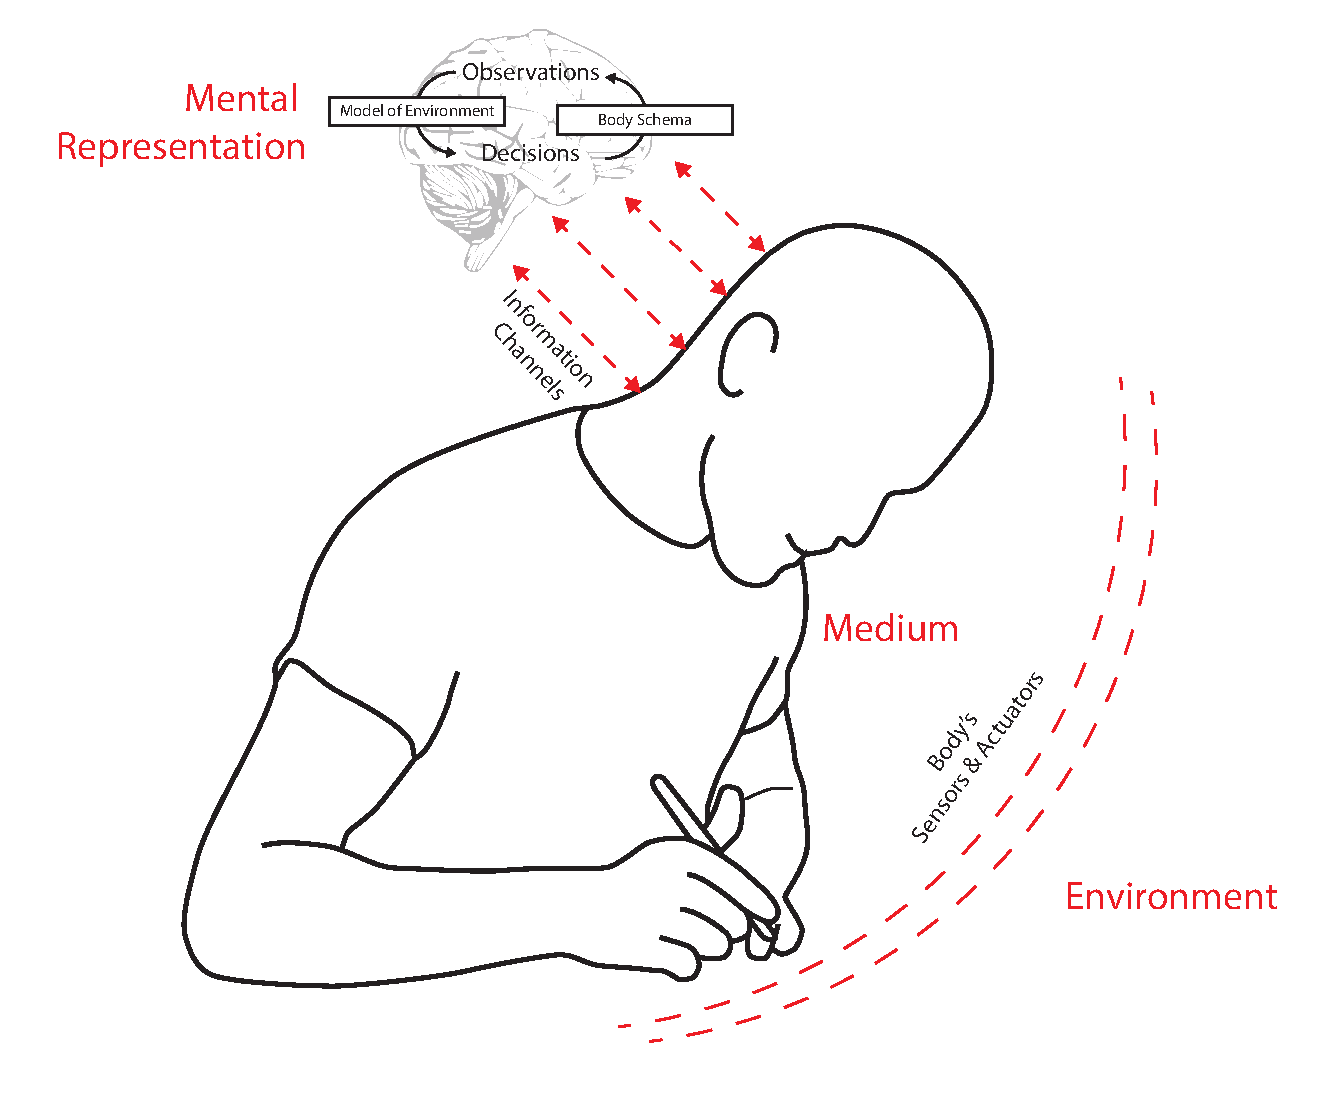
\includegraphics[width=0.75\linewidth]{figures/intro/BodyInteraction.pdf}
  \captionsetup{justification=centering}
  \caption{Body schema is a constant internal process representing the medium of interaction (body).}
  \label{fig:intro-bodymodel}
\end{figure}

Body Schema involves aspects of both brain processing and body peripheral (Proprioception signals, sensory signals), and it is considered as a collection of processes that stores the posture of the body and relationship of body and its representation. When the body state became in motion, the body schema updates unconsciously according to that motion \cite{holmes2004body}. A mental image maintains a constant representation of the body while a task is being carried on \Figure{fig:intro-bodymodel}. The observations/decision loop which is unconsciously updating our mental representation relies mainly on the information channels that interact with the body. In some sense, its possible to represents the body as being a medium between the internal mental image, and the surrounding environment in which the body is located at, and at which the task is being performed in. 

The idea of the body schema and the mental image of the body has been derived from philosophical and empirical perspectives. Aristotle in his book (On The Soul, II) referred to the soul as being the form of the physical body, which perishes together with it at the death. And according to Spinoza (The Ethics, II) said the soul is the \textit{idea} that the body develops of itself. In a modern term, the \textit{idea} is simply a mental representation, more precisely, a self-representation. Gestalt properties, such as body shape, are rather global properties of the entity, and thus the body schema or the self-representation is being a neural mechanism to represent exactly such global properties. In a modern philosophy, Matzinger \cite{metzinger2007empirical} has presented that the body and self can be a plastic representation and highly context sensitive. He referred to the self-representation with the concept of ``Self-model'', which is a process driven by a series of cross-modal interactions from the several sensory channels in order to define the image of self and body. For example, in the rubber-hand illusion (RHI) \cite{botvinick1998rubber}, the sensation of being stroked with a prob is integrated with visual and kinesthetic feedback in order for the brain to constructs a matching proprioceptive map between the subject's mental image of his body and what he perceived from the sensory channels. As a result, the subject's mental image of the body ownership is redefined and would then believe the rubber hand is part of his body. This illusion is extended to modulate the body schema to perceive a third arm as being a part of the body \cite{guterstam2011illusion}.

By considering \textit{the body as a medium for interaction}, then its possible to create a proxy that maps the sensors and actuators of the body into a different representation. In Telexistence, previous research showed the possibility to transfer body awareness using a remotely operated avatar matching operator's body schema \cite{fernando2013design}. A visual-kinesthetic transfer model is defined to create the sense of bodily presence and ownership toward the remote representation. And fundamental elements for presence, such as vision matching, real-time control and operation, and tactile feedback, are important elements in creating such a schema transfer model. By maintaining such baselines for presence, and defining a top-level model to remap the other modalities, it would become possible to redefine body schema while preserving the sense of ownership toward the alternative representation.


Within the scope of this thesis, Embodiment emphasizes the role of the body in defining and shaping the mind and its cognition through the sensory-motor skills being performed, and the sensory-perceptual inputs being perceived. That is, the body is being the medium and the interface of the mind.

\subsection{Isolated Modalities}

A modality can be considered as a single independent channel of sensory input/output between human and the surrounding environment. As in our daily interaction, we rely on cross-modalities to have a clear comprehension of the tasks we involved in. Human body physical structure imposes tight coupling of these modalities, and our mental representation is mapped to this tight coupling. However this tight coupling can introduce an overlapping information, and some of the sensory inputs are not necessary for the task being involved with or would result in sensory distraction between the various sensory modalities.

%\begin{comment}
Isolating the involved modalities for a specific task would enhance the operation and achieve a higher sense of \textit{attention} by reducing non-relative sensory and perceptual information (distraction).

\begin{quote}
``Everyone knows what attention is. It is taking possession of the mind, in clear and vivid form, of one out of what seems several simultaneously possible objects or trains of thought. Focalization, concentration of consciousness are of its essence. It implies withdrawal from some things in order to deal effectively with others, and is a condition which has a real opposite in the confused, dazed, scatter-brained state which in French is called distraction, and Zerstreutheit in German.''  (William James - The Principles of Psychology Vol. 1 1980 p.404)
\end{quote}

In his definition of \textit{Attention}, James highlights the role of isolation of a sensory stimulus through the concentration towards it in order to effectively engage in or observe from a certain action.

\begin{comment}
As an example, libraries in a sense removes the distracting auditory noise and ban them so the scholars in the library can focus or immerse themselves in reading. Similarly in cinema theaters in which also the customers tend to concentrate and engage with the provided contents.
\end{comment}


\begin{figure}[t!]
  \centering
	  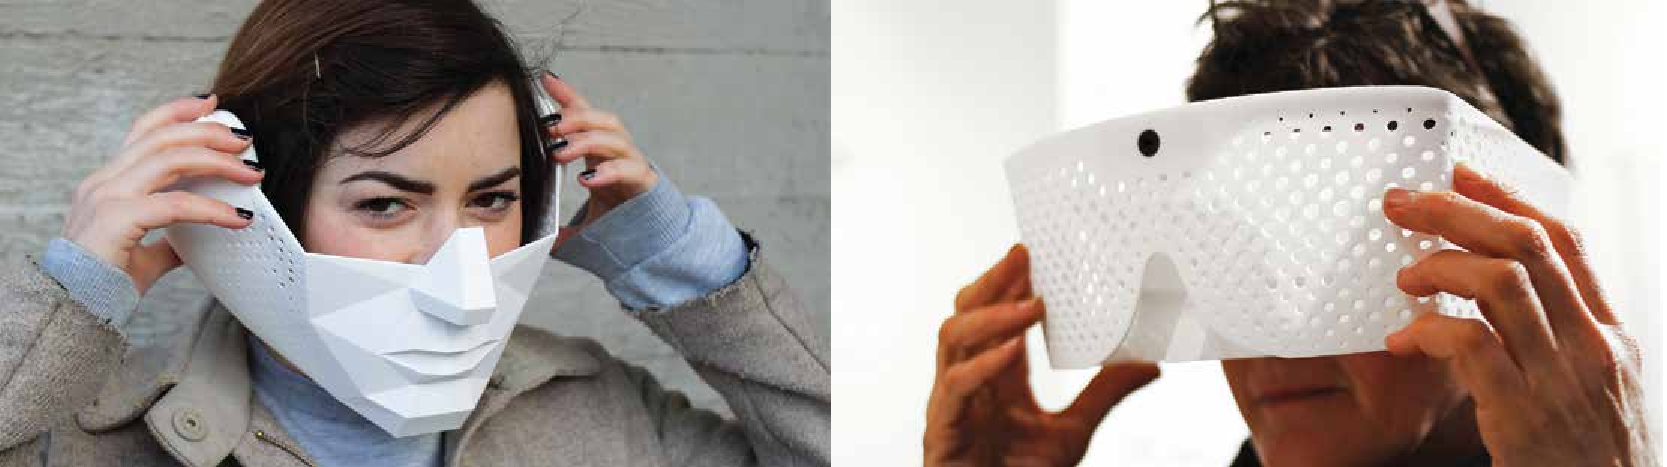
\includegraphics[width=1\linewidth]{figures/intro/Eidos.pdf}
  \captionsetup{justification=centering}
  \caption{Enhancing perceptual modalities using wearable devices. Eidos Audio (left), and Eidos Vision (right). }
  \label{fig:intro-eidos}
  \text{\footnotesize Photo \copyright\xspace Eidos (2012).}
\end{figure}

Abstracting the individual modalities, based on their function and type of information they carry, would assist the design and use of digital tools and media to enhance them individually, and then provide their contents back to the user through feedback devices. Eidos \cite{tim2012eidos} shown in \Figure{fig:intro-eidos}, illustrates the possibility of controlling our individual senses and adjusting them separately reducing other distracting information. Isolated modalities based design helps enhancing individual modalities functions, or even achieve supernatural capabilities such as augmenting visual perception \cite{koizumi2012stop}. 


\subsection{Body Ownership}
In order to establish that our perception of body and self can be altered via modifications of our sensory modalities and embodied representation, psychological studies and empirical evidence are required to support this claim. Previously we discussed the phenomena of rubber hand illusion which can create a strong sense of ownership to an artificial body based on the cross-modality experience of vision and haptic feedback. That example showed how the perception of body part ownership can be altered through external stimuli. 

In a contrasting example of altering the sense of body ownership: the phantom limb sensation \cite{melzack1992phantom}. In this phenomena, a person perceives a missing arm or leg as still existing regardless of the fact that it's being not physically present. That is, their mental image of their body still poses the perception of the capability of moving the limb, the proprioception feeling of its posture, but without visual or tactile feedback from the missing limb. This inconsistency of perceptual feedback with the internal mental image of the body causes what is called phantom limb pain. In one of the previous studies on the phantom limb pain treatment, the visual illusion of missing limb was 'resurrected' back to the patient using a mirror setup \cite{ramachandran1995touching} in which the patent sees his functioning limb in the location of the missing limb. An illusion of kinesthetic sensation emerged during the trials, even when the experimental used his hand instead of the patent hand to induce this sensation. 



%Where Am I by Daniel Dennett 1981
%Chapter 3 discusses further details about \ProposalKeyword for body mapping using modalities input/output channels. Also, a Telexistence Toolkit is proposed as a proof of concept. The toolkit provides hardware set which can be used along a meta-modeling software for defining the relationships between operation and representation.

\subsection{Modalities Substitution}

Brain plasticity and adaptability to modulate sensory feedback and restructure the perceptual awareness has been widely investigated in psychology and neurology. A subset of this area of research is modalities or sensory substitution. This research involves the study of the effective sensory modalities that can be used to replace another one. Thus the research involves the study of meaningful conversion of the information from one modality to another, and the representation used to deliver the newly converted information.

In neurology area of study in sensory substitution systems, a person who lost a certain sensory due to peripheral damage still has the capacity to sense within his brain structure. For example, for a blind person, the peripheral sensory system (retina) is not functional which results the fact of blindness is still has the capacity to ``see'' from neurological perspective unless if the visual cortex of the brain is damaged. Similarly for those with positional orientation and balance disorders (the vestibular apparatus), or deaf due to sound transduction damage in the ear (the cochlea). Previous work \cite{bach1972brain, bach1995nonsynaptic} found that the input from a sensory substitution system can stimulate the brain regions which lost its sensory peripheral. 

\begin{figure}[b!]
  \centering
	  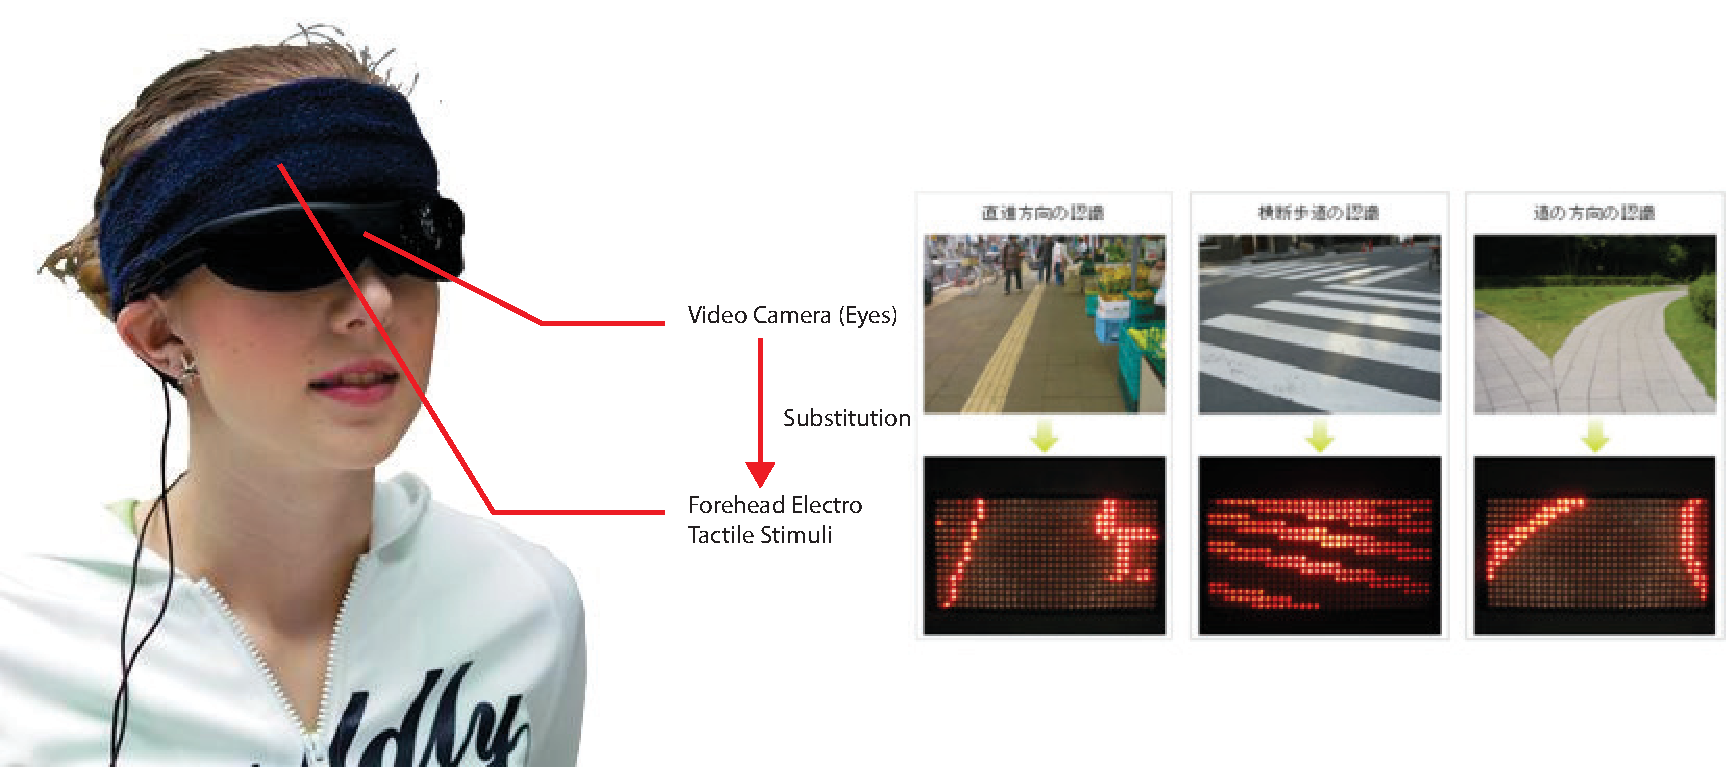
\includegraphics[width=1\linewidth]{figures/intro/SSD.pdf}
  \captionsetup{justification=centering}
  \caption{Visual sensory substitution using tactile feedback }
  \label{fig:intro-SSD}
  \text{\footnotesize Photo \copyright\xspace AuxDeco, Inc (modified from original)}
\end{figure}

Sensory substitution devices (SSDs) have been commonly used as means of non-invasive methods to restore a certain sense of the surroundings. SSDs are generally divided into two main variations: visual-to-tactile substitution devices that translates optical information into tactile stimuli, and visual-to-auditory substitution devices that convert sound into an audio wave. Widely used is the tactile based SSDs to restore the visual modality for blind people, and as one of the earliest examples of such tools is the white cane which still being used until now by blind people (recently proposed EyeCane \cite{maidenbaum2014eyecane} augmenting the traditional white cane). Braille is another commonly used SSD to provide tactile amount of information of written symbols. White et.al \cite{white1970seeing} developed a tactile SSD that converts the optical images captured by a camera into an input to an array of solenoid vibrators located on the back of the user to induce visual information through tactile sensory channels. Commercial products that use electro-tactile stimuli to substitute the visual modality has been also introduced previously, AuxDeco by EyePlus-Plus Co. Inc \cite{auxdeco} uses forehead as input surface for the visual information, while BrainPort by Wicab Inc. \cite{brainport} uses the tongue. The other spectrum of SSDs used auditory feedback. As one of the very first SSDs is ``Ultrasonic Eyeglasses for the Blind'' proposed by Leslie Kay \cite{kay1973sonic} which is a biomimicry glasses that uses ultrasonic sensors to measure the distance and the geometry of the objects, and produces auditory tones that vary in frequency depending on the distance. More recently, the vOICe by MetaModel Inc. \cite{vOICe} uses the audio modality as a substitution to the vision by converting visual stimuli into musical notes. Other variations of vision-to-auditory approaches to transform the image data have been widely investigated \cite{meijer1992experimental,capelle1998real,hanneton2010vibe} which are not only used for visually impaired people, but also as approaches to transform visual information to meaningful auditory information.


\begin{comment}
%Substitutional Reality, not clear if it links in this context
A recent variation of perceptual substitution is the reality substitution. Substitutional Realities (SR) was first coined by Suzuki et.al \cite{suzuki2012substitutional}, in which a proof of concept system was developed. As in conventional modality substitution systems discussed before, the SS system is used to replicate the input of a lost modality using a different sensory peripheral, in SR the sense of reality and time is being substituted with an alternative pre-recorded visual feedback input. The approach of SR is to blend in and out the real-time and past recording in a controlled condition which might involve physical interactions between the experimenter and the participant in real-time period convincing the participant of the physical presence. The pre-recorded visuals is done from the same point of view of the participant's eyes in omni-directional manner, thus when the blending with the past occurs, the participant maintains consistent flow of information along his head motion. Under controlled conditions, SR proved that the sense of presence is possible to alternate using single modality substitution. The participants expressed high level of confusion of whether what they see is happening in real-time within their spatial bounds. Derivations of SR has also been proposed, Reality Jockey \cite{fan2013reality} in which the focus was on auditory modality substitution, and \cite{simeone2015substitutional} which uses physical/virtual space substitution to enhance the bodily experience of presence in virtual reality applications. Blended Reality \cite{kevin2017blended} expands on SR topic to address the variations of presence substitution in terms of time, space, and modalities.
\end{comment}

\subsection{Body Morphology}

\begin{figure}[b!]
  \centering
    \centerline{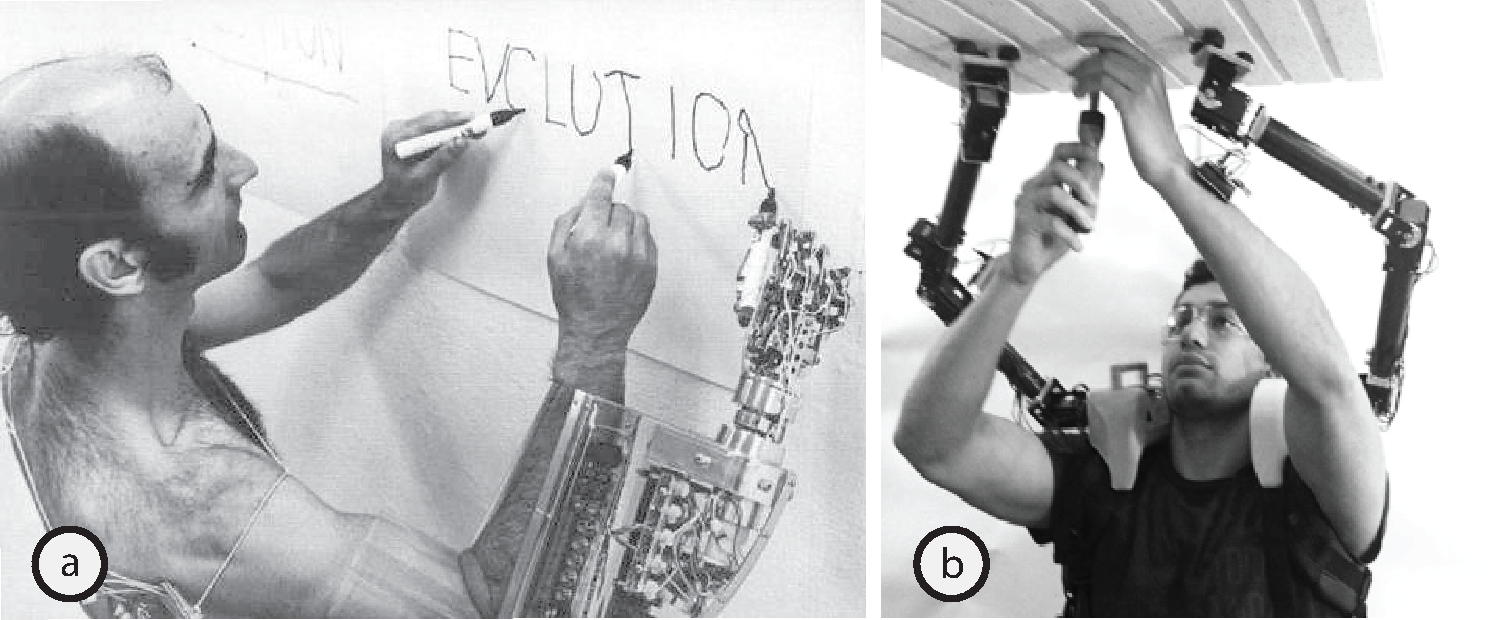
\includegraphics[width=1\linewidth]{figures/intro/BodyExtension.pdf}}
  \captionsetup{justification=centering}
  \caption{Body physical morphology using additional limbs. (a) Stelarc Third Hand motion is driven from body muscles, where (b) MIT's Supernumerary Robotic Limbs (SRL) action are application driven.}
  \text{\footnotesize Photo \copyright\xspace (a) Stelarc, and (b) MIT Federico Parietti.}
  \label{fig:intro-bodyext}
\end{figure}

To overcome the rigidity in physical constraints our body schema constitutes, first a digitization of our body's sensory and actuating modalities is needed. The conversion from analog/physical representation into a digital form would provide the required flexibility to remap, augment, and alternate what we observe and how we operate. The process of digitization of the body can be done using sensors to track the different types of actuation body presents, and perceptual proxies devices which produce different types of sensory feedback to the body. As seen in the previous section, the sensory feedback can be modulated or substituted before providing it to the user's body in order to overcome a certain disability or to augment a modality. Such process will be referred to as modality transfer.

Modality transfer can be seen in two types: Local schema transfer when the medium of interaction is spatially located along the body so its modalities are cooperating with the alternative modalities used to shape the body schema. And remote schema transfer when the medium of interaction extends spatially into a different location, thus the cognition relies completely on the used representation to communicate with the environment. 

In local schema transfer, it is possible to induce new body schema when we use tools that, for example, shift the function of the modality in a constant manner. For example, when using a pen for writing, the pen becomes an embodiment of an object with the functionality to point, write, and touch. When we adapt to the use of the tool, it becomes transparent and a part of our new body schema. Robotics has been used also to reshape our functions in an embodied or assistive manner \Figure{fig:intro-bodyext}. Stelarc Third Hand \cite{kac1997foundation} was one of the first ``successful'' trials to embody an extra robotic prosthesis to his biological body. The prosthesis was physically strapped into his right arm, but had functions to grasp, pinch, and rotate its wrist. The arm is considered as being embodied because its motion was driven from his bodily functions, that were EMG\footnote{Electromyography which records muscle activities using electrodes placed on a relevant skin surface.} signals from his legs and abdomen. The EMG signals acted as a real-time digitization of some functions of his body which served to be a transparent channel communicating with the prostheses. This bodily driven control allowed him after many years of use to adapt this arm to his body schema, and to operate it as an extension of his body \cite{stelarc1980thirdhand}. On the other hand, other types of tools are considered as assistive rather than being embodied with the human body, such an example is the Supernumerary Robotics (SR) \cite{llorens2012based,bonilla2014robot, parietti2014bracing, wu2014bio}. Such type of SR systems are designed to work side by side with a human operator in a coordinated manner, it has an independent behavior when performing the tasks to optimize the operation which the human is performing through independent observations and reactions. Thus its motion is not driven by direct bodily actions, but rather from the task's context, which means the arms could be considered as a separate entity disembodied from the human operator.

\begin{figure}[htpb]
  \centering
	  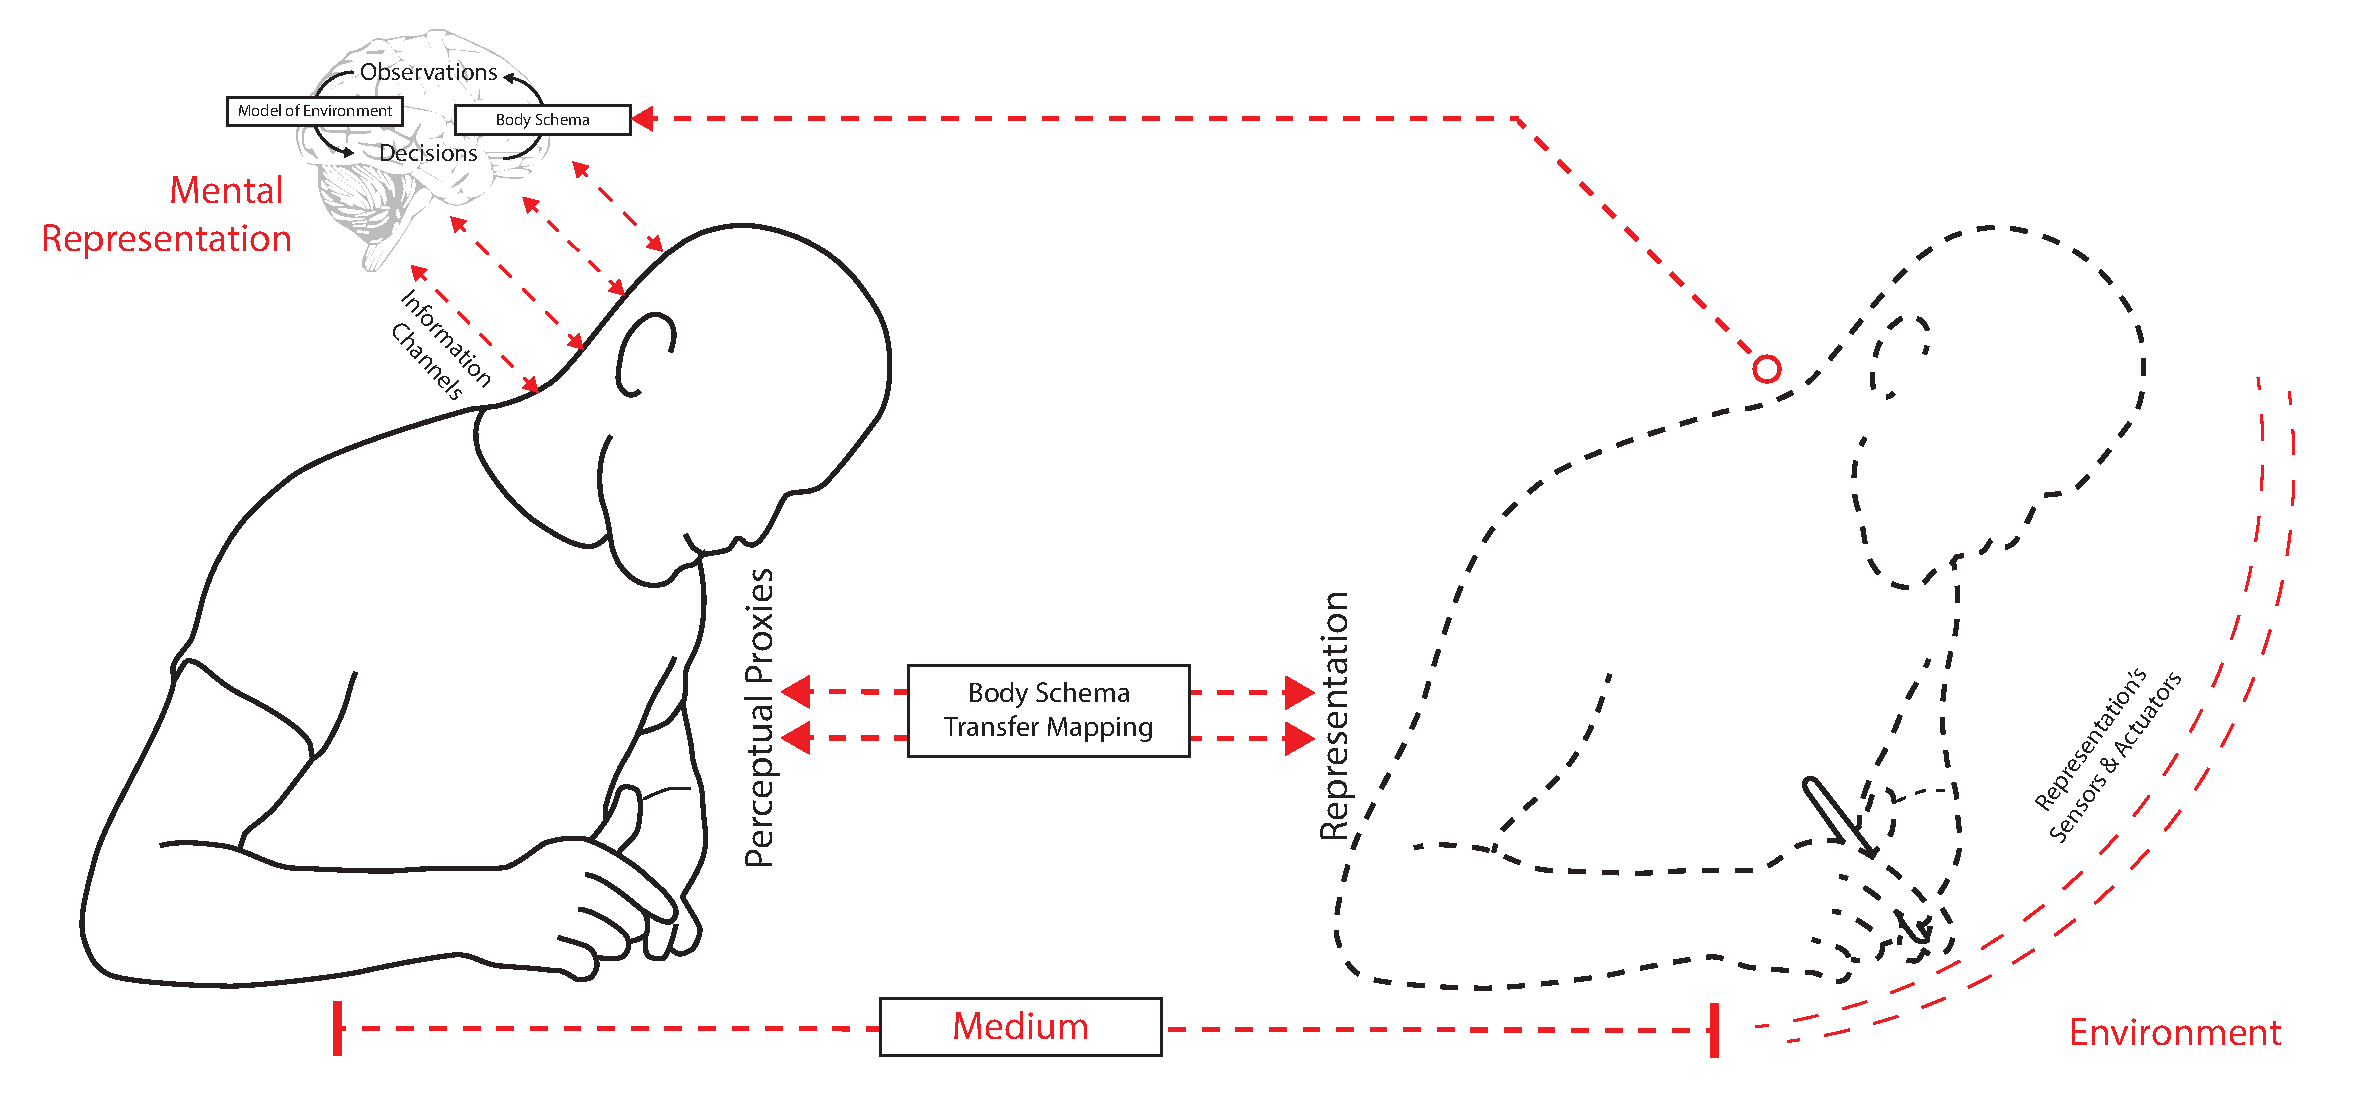
\includegraphics[width=1\linewidth]{figures/intro/representation.pdf}
  \captionsetup{justification=centering}
  \caption{An overview of the process of digitizing human body perception, and extending the medium of interaction (human body) into an alternated representation. Body modalities are transferred into an alternative representation.}
  \label{fig:intro-digitalRep}
\end{figure}

For remote schema transfer, the process of body schema adaptation requires the modalities to be transferred from one location to another by digitizing their functions so its possible to capture and reproduce them from one side to another. \Figure{fig:intro-digitalRep} provides an overview of the process of digitizing body schema, and transferring it from an alternative representation into the body via perceptual proxies. Body schema transfer mapping block acts as a definition for the process of real-time updating the representation with the human body using the digitized sensory channels. Work in telepresence and telexistence derives similar approach for creating a sense of presence in a remote environment for teleoperation purpose. These approaches, as will be discussed in the next section, transfer the body modalities from one location to another to stimulate the sense of remote presence.
%Previous work showed that our mind has the plasticity to continuously shaped and re-shaped to new body representations, for example, to embody different body \cite{peck2013putting}, or to alter the physical properties of the body \cite{rosenberg2013virtual}.  



In conclusion, in order to alternate body schema, there should be a consistency of sensory inputs regardless of the physicality of the observed body or the representation, thus maintaining the sense of ownership. Also, to preserve the sense of agency towards the body, the observations from the body (e.g. movement) should be correlated with the actions of the user. 


%%%%%%%%%%%%%%%%%%%%%%%%%%%%%%%%%%%%%%%%%%%%%%%%%%%%%%%%%%%%%%%%%%%%%%%%%%%%%%%%%%%%%%%%%%%%%%%%
\section{Presence Augmentation \& alteration}

In this section, discussion about related work in body presence augmentation and alteration. Work in Telepresence, Telexistence, and spatial awareness are described showing the impact of such means to expand body's limited perception and actions. 

\subsection{The Essence of Presence}

Presence is the state of awareness of body and its surroundings. Enhancing the state of presence or altering it is to change the physical constraints or to convince the mind of being at a different state than what the body physically is. Kim \cite{kim1996effects} highlights on that as ``feeling of being a part of the phenomenal environment created by television and not being a part of the physical environment surrounding the viewer and the television set''. Similarly, with the use of virtual reality tools, it's possible to lead the mind into a ``suspension of disbelief that they are in a world other than where their real bodies are located''\cite{slater1993representations}. The state of presence is a flexible term that can stretch over time and space, as well as the form of body perceiving the various sensory modalities which develop the understanding of where and how the body is located at. 

In physically teleoperated environments, several work and research discussed the requirements to provide a physical presence to operate and to be embodied (as being part of the remote location). Minsky \cite{minsky1980telepresence} proposed telepresence systems that function to provide ``feeling like you are actually 'there' at the remote site of operation''. Minsky highlighted the role of teleoperated systems to empower the functions of human operation and labor to perform an effective operation for the tasks at hand. The essence of providing the sense of transferring body awareness to remote slave system was proposed by Tachi in his paper on Telexistence systems  \cite{tachi1985tele}.  ``a system that at the remote control-site a human operator can perform remote manipulation tasks dexterously with the feeling that s/he exists in the slave anthropomorphic robot in the remote environment.'' which is referred to as Tele-existence system (or Telexistence) under the condition of  ``real-time sensation of remote presence''. This definition provided a requirement of the subjective experience of body presence ``...perform remote manipulation tasks dexterously with the feeling that s/he exists in the slave...''. The requirement of mapping and matching the state of the body between the human operator and the slave system creates a strong sensation of agency and ownership. Rheingold \cite{rheingold1991virtual} described Telexistence systems as a ``form of out-of-the-body experience'' once he looked at himself through the slave system. Telexistece systems can be viewed as a way of presence augmentation since the body's physical constraints are extended over distance, and the effect of manipulation and perceiving can be done remotely. The usage of mediated technologies can help to reproduce the sense of presence, and thus can be a mean to enhance and alter this sensation.

State of presence can also be stretched to non-physical environments. Virtual presence is usually regarded to the state of being in a non-tangible space which is being represented by digital means. Sheridan \cite{sheridan1992musings} created the distinction between physical and virtual, in which physical presence is characterized as ``physically being there'' while virtual presence as ``feeling like you are present in the environment generated by the computer''. The master/slave system of Telexistence also proposed to operate under virtual environments as if being in a physical one \cite{tachi1991tele}, extending the concept of presence into virtual, non-physical spaces.

\pagebreak
\subsection{Connected Awareness}


\begin{shaded}
\begin{quote}
\textit{
\centering{\textbf{The story of ``Waldo''}}\\
%http://cyberneticzoo.com/teleoperators/1942-waldo-and-waldoes/
``Waldo'', a fictional novel by Robert A. Heinlein 1945 \cite{heinlein1942waldo}, tells a story of a mechanical genius who lived his entire life in a self-imposed exile: his own body. Struck with a neuromuscular disease (myasthenia gravis) in which it locked him inside the shell of his weak body, he was capable to develop dozen of mechanical hands (called as Waldo F. Jones Synchronous Reduplicating Pantograph) which are operated via sensory devices attached to his hands, and extend his body and enable him to amplify his weakened muscular strength. These mechanical hands were depicted as in various sizes which can be as small as micrometers in span allowing him to micro-manipulate, and all the way up to six meters from finger to thumb in size allowing him construct buildings and facilities while imitating his hands motion and actions. Despite of the fact of being crippled in his weakened body, Waldo considered himself as a superior to humanity since his augmented skills and his body extensions enabled and empowered him to do far more superior tasks than what a fully functional human can do. 
}


\end{quote}
\end{shaded}

The story is considered as one of the very first original novels which highlight the effect of technology and tele-body-representations to augment the motor skills of our bodies. Also, it highlights the effective adaptation of connected bodies and awareness to amplify our cognitive skills and enhance our physical capabilities. 

Thanks to the never-ending expansion of interconnected networks and Internet, the boundaries of location and space has expanded from local to a global scale and created a true ubiquitous information accessibility. Mark Wiser\cite{weiser1994ubiquitous} introduction to Ubiquitous Computing helped to create a new paradigm of information accessibility and networked computational design. These technical innovations in network media and information accessibility opened a wide door for the emergence of digital-based Teleconferencing and Teleoperation tools at a wider scale compared to the older analog-based media transmission. These tools provided the capability of transporting human beings virtually from one place to another to get involved in a remote discussion, or to transport his skills for solving remote tasks. 

\begin{comment}
Back in 1980s, Susumu Tachi \cite{tachi2016telexistence} \& Marvin Minsky \cite{minsky1980telepresence}, both scientists \&  visioners from the east and the west proposed the means and concepts of the tools and medium which human operator can use in order to have the awareness of the distant location. There is a fundamental difference between the concepts proposed by Minsky (Telepresence) and Tachi (Telexistence). The former concept focuses on the tools to operate remotely and on the quality of remote task, however, the latter one addresses cognitive and awareness related factors for the quality of operation and sense of presence. Each of the previous teleoperation approaches has a different aim \Figure{fig:intro-tele}, the former is task transfer oriented approach, while the latter is body transfer oriented approach. For the human operator, it helps to have a sort of Teleportation from one place to another instantly and to avoid any risk of exposing his biological body into a hazardous environment which the avatar can be located at. Also, it transports the knowledge and expertise of the user instead of using Artificial Intelligence based robots. 
\end{comment}
%require to cite a work about self-consciousness \cite{lenggenhager2009spatial} before talking about telepresence systems

\begin{figure}[!ht]
  \centering
  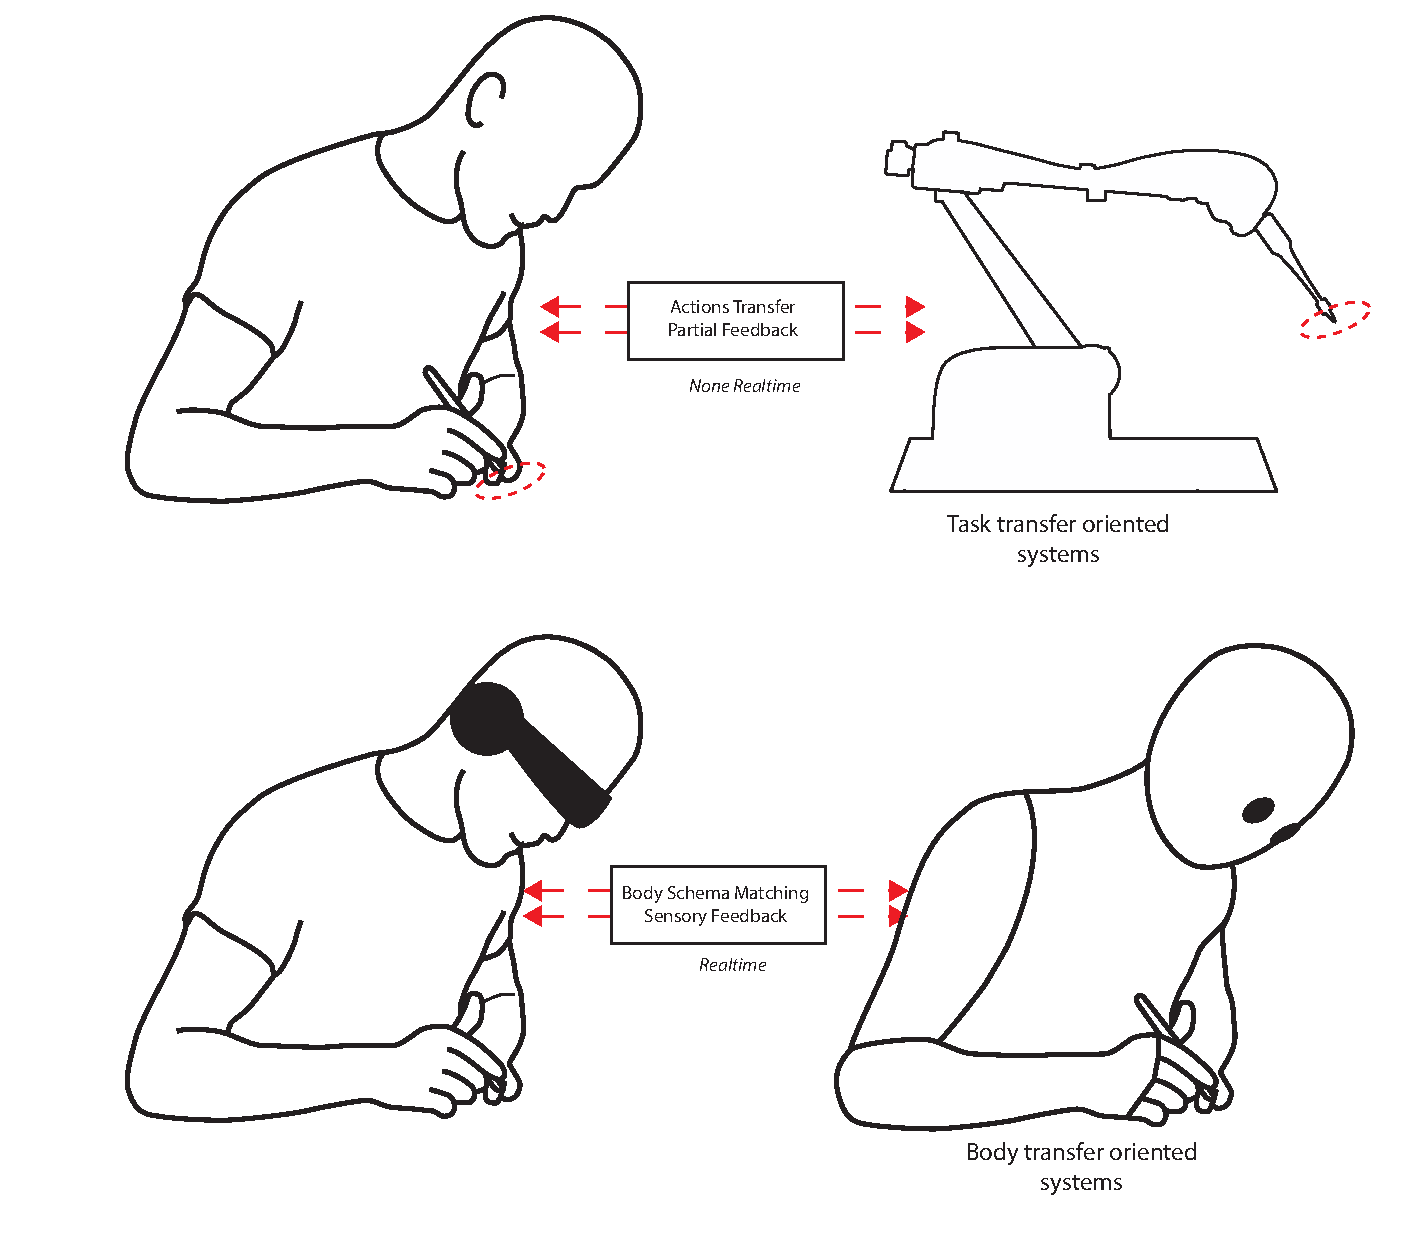
\includegraphics[width=1\linewidth]{figures/intro/Teleoperation.pdf}
  \captionsetup{justification=centering}
  \caption{Task vs Body transfer oriented systems. }
  \label{fig:intro-tele}
\end{figure}


Basic teleconferencing tools, such as Polycom video conferencing \cite{rodman2004polycom}, Skype, and Google Hangouts provide an easy to use means to connect remotely, however they lack to represent the physical attributes of the operator, and rather have limited number of modalities that are engaged (commonly video/audio feedback). The other paradigm aside from the basic teleconferencing tools could be categorized to Telepresence and Telexistence technologies \Figure{fig:intro-tele}. Each of these addresses different type of cognitive transfer, the prior is task transfer and the latter is body transfer.

Telepresence systems emerged to the market and gave higher levels of flexibility for operation and representation, such as MeBot \cite{adalgeirsson2010mebot}, Kubi \cite{kubi2013}, and Double Robotics \cite{robotics2015double}. These systems would allow motion and teleoperation and even can transfer non-verbal cues via robotics hands, or facial expressions \cite{misawa2013livemask}. Telepresence systems, in general, can be referred as task transfer-oriented systems, which focuses on the use cases of the system instead of the full embodiment of the operator.

\begin{figure}[htpb]
  \centering
  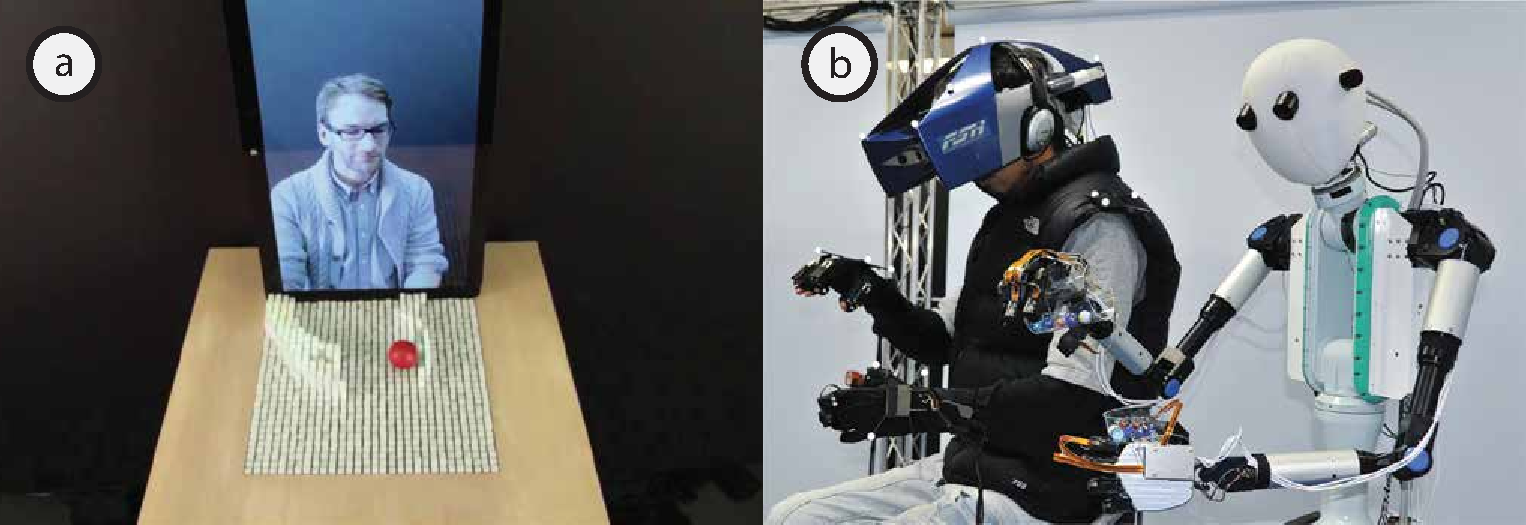
\includegraphics[width=1\linewidth]{figures/intro/TeleTech.pdf}
  \captionsetup{justification=centering}
  \caption{Embodying teleoperation technologies (A) inFORM as an example of Telepresence systems, and (B) Telesar 5 as an example of Telexistence systems.}
  \label{fig:intro-tele}
  \text{\footnotesize Photo \copyright\xspace (a) MIT Tangible Media Group, and (b) Tachilab.}
\end{figure}

In Telexistence related applications, an avatar that represents a substitute representation of human body using robotic systems and digital forms, the human operator can remotely access and have immediate control and real-time feedback sensation from the remote surroundings as if the operator is actually located there. Although current Telexistence systems \cite{tachi1985tele,tachi1990tele, hasunuma1999development,kawakami2005telesarphone,watanabe2007torso,fernando2012iros} provide a partial representation of the human body, however, they achieve a strong sense of self-consciousness and sense of presence in the remote place, which Telepresence systems lack.

%Both Telexistence and Telepresence are solid implementations of that novel.

In some sense, we can say that both Telepresence and Telexistence systems are a one-to-one mapping of the user to his avatar (best case when a full body representation is achieved). Based on this definition, although avatar representation provides enhancements to the human operator and overcomes several difficulties that direct human operation cannot serve, these methods of direct one-to-one mapping has upper bounds of what an augmented human can do. The question is, what happens if a physically disabled person tried to use such systems? As its a direct one-to-one mapping, the disability will also arise in the representation too. In Waldo's case, his body was weak but not disabled, and his hands were still being represented as direct one-to-one mapping with his waldos. Without his basic motor skills, he would not be able to operate the body amplifiers he invented.


\subsection{Presence Embodiment}

Media interfaces are progressively growing to embody us within it, affecting our sensations of physical presence, social presence, and self-presence inside. This progression in telecommunication technologies creates a tighter coupling between the body and the interface, in which the body becomes a part of the physical space and the cyberspace. This progression creates an adaptation between the body and the interface \cite{biocca1997cyborg}. Adding to that, research in Virtual Reality and cognition showed that sense of presence can be provided through technical means and psychological experiences \cite{riva2006communication}. Technological means are the physical representation of sensory organs, such as stereo vision (eyes), binaural audio array (ears), tactile system (touch), ..etc. The psychological experiences define the relationship between the technological means and the human body. Thus by altering both the means and the experience, sense of presence can be altered or enhanced, while maintaining the seamless experience of presence, or of being there.


\subsection{Beyond Presence}

The question of the possibility to leverage what our bodies can perform, or expand the perceptual capabilities of our visual, auditory, and tactile modalities has been a focus in human augmentation research area.

Recent systems were introduced to share the presence, and can be sort of extension of telepresence systems. Kasahara \cite{kasahara2014jackin} proposed a JackIn system to allow vision sharing, thus enhancing participants bodily and visual presence into being remotely presented. An extension of this work \cite{kasahara2016parallel} is to share vision into multiple locations, thus multi-casting the presence. Cohen \cite{cohen2007multiuser,cohen2009awareware} proposed to use an architecture of sources and sinks to direct the auditory feedback from multiple sources into a single observer. Although this architecture does not define a general way of mixing or layering information from these multiple sources, it proposes a framework for multi-sensory feedback systems and can be viewed as a way of presence alteration.

Recent research builds on these tools in order to enhance the presence and expand body's perception. Fan et. al \cite{fan2014acm} proposed a video-based image blending using two-way see-through HMD that provides the user an awareness of both locations behind and front of him by blending the visuals of both views. This type of augmentation can be viewed as remapping vision modality into multiple channels of input. Suzuki et. al \cite{suzuki2012substitutional} used pre-recorded 360 visuals and blend it using see-through HMD by phasing the visuals in and out through a specific scenario resulting the user experiencing past as being present, and thus altering the sense of presence for the user.




\begin{comment}

For operator side, when a perceptual device is used such as HMD, his body visuals are occluded and instead he would perceive the remote robotic representation. This kind of representation would cause a disconnection of the presence, and the user would be aware of being just operating rather than of ``being there''. To present user's body visuals into a virtual environment, several work investigated the appropriate methods to achieve that using image-based segmentation of operator's body. Yokokohji \cite{yokokohji1996you} developed a ``What you can see is what you can feel'' system, which is used to present operator body visuals by segmenting the first point of view images and overlaying them into user's display. Bruder \cite{bruder2009enhancing} used egocentric images of user's body which are captured using a video-see-through HMD, and superimposed the segmented hands into virtual environment visuals. Tecchia \cite{tecchia20123d}, demonstrated the usage of depth array sensor to capture user's hands interaction and superimpose it remotely for visual guidance applications.
\end{comment}




\section{Meta-Modeling Design}

In this thesis, a design approach is proposed in \Chapter{ch:concept} for Embodied-Driven Design to define the body transfer and schema. This section provides a brief overview of the related work and research that uses meta level modeling approaches in various design fields, and gives the necessity of adapting relevant approaches for the proposed meta-modeling environment. 

The idea of using tools such as diagrams for abstraction and modeling has been a commonly adopted approach to provide a middle ground between engineers and designers, and as tools for quick prototyping and re-usability of previous models. This can be attributed to the simplification of the target system or interaction, avoiding the designer to be involved in technical details thus attracting a wider audience to adapt to the tools. The original idea of visual programming was proposed by \cite{shu1988visual} to address the previous concerns. Max/MSP \cite{puckette1990max} and Pure-data \cite{puckette1997pure} uses visual programming approach for modeling, and they are widely used by designers who do not have programming skills, like audio or visual designers, accelerating their prototyping and testing process. These approaches have also been adapted for educational purposes due to the easiness, symbolic representation, and immediate results when performing actions within the model. Scratch \cite{maloney2010scratch}, LittleBits \cite{bdeir2011electronics}, and MakerWear \cite{kazemitabaar2017makerwear} used similar approaches for children oriented workshops using tangible or on-screen charts. 

%\pagebreak
\section{Impact of the Proposed Research}

By the time of writing this thesis, there has been no known method or tool which provides the possibility to redefine the function of human body, or rewiring the body functions with external tools. The work established in the area of human augmentation has been mainly function driven, that is a bottom-up approach to the design of the systems.

Embodied-Driven Design builds on the research area described previously, and it provides a unified framework for defining and forming a systematic representation of the human body and its representation. Body representation and the way its mapped to operator's body plays an important role to maintain or enhance the presence experience and thus the operation quality. Embodied-Driven Design addresses this point by providing body schema transfer blocks into physical/virtual or hybrid representations. Physical representation blocks provide essential modalities for remote presence, such as visual/auditory feedback, physical interaction, and so on. Virtual representation blocks provide the capability to deform body visuals remotely to enable non-physical interactions, or to substitute available physical representations remotely, such as hands representation.  

 % 8 pages --> 10~12 pages

\pagebreak
%\cleartoleftpage
\epigraphhead[400]{
\centering\textit{
``Our Bodies are the Medium of Interaction, \\the Bridge of our Minds''}}
\part{Embodied-Driven Design}
\label{pt:II}
\pagebreak
\chapter{Concept \& Design Strategy}
\label{ch:concept}

\markboth{Embodied-Driven Design}{}

\begin{flushright}
\textit{
``one sees the environment not just with the eyes, but with the eyes in the head on the shoulders of a body that gets about. We look at details with the eyes, but we also look around with the mobile head, and we go-and-look with the mobile body''}
\par\hfill\textsc{James J. Gibson, The Ecological Approach to Visual Perception 1979}


\end{flushright}
\vspace{15pt}

%\section{Overview}
\begin{comment}
\begin{wrapfigure}[23]{r}{0.41\textwidth}
  \captionsetup{justification=centering}
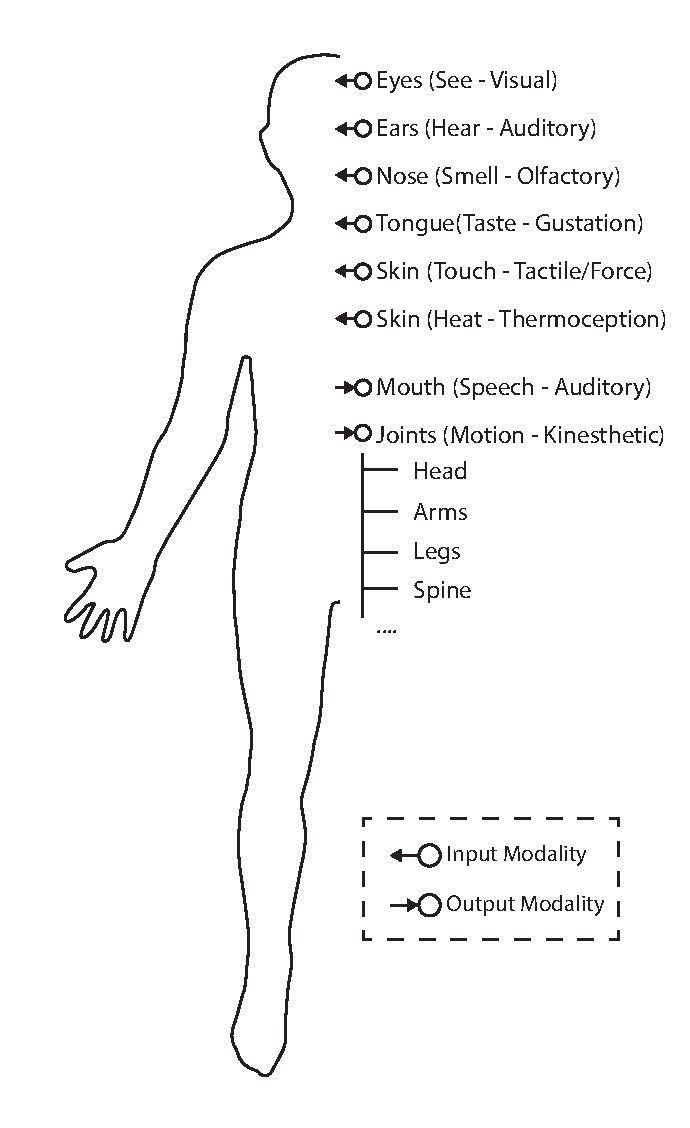
\includegraphics[width=0.35\textwidth]{figures/concept/Modalities.pdf}
\caption{Human Body Input/Output Modalities}
  \label{fig:intro-modalities}
\end{wrapfigure}


The idea of Embodied-Driven Design relies on the possibility of reconfiguring our body schema mapping and structure using mediated representation in the remote location. But before diving into the topic of body schema design and reconfiguration, a base design pattern is necessary to be described. Loosely-Couple Modalities (LCM) design pattern is the fundamental block in the design process of body schema reconfiguration. Using this design pattern, it's possible to simplify the body structure and the involved modalities in the target teleoperated task or goal representation. Using this design pattern, its possible to reconfigure the body schema using an Embodied-Driven Design framework. 

\end{comment}
%Chapter 2 has introduced the fundamental background of Embodied-Driven Design
This chapter will address the design aspects and process for body driven applications by first providing a systematic model of human body schema, and then deriving topological models for the postural and sensory body schema. The idea of decoupling and re-coupling is also discussed here as a part of LCM design pattern which allows the reconfiguration of body schema mapping by using a topology of the various body modalities. And finally, EDD framework is described along with the meta-modeling tools and modular blocks that reflects LCM design pattern. Three meta-modeling design categories are discussed that summarizes the major use-cases and design scenarios that EDD can serve. To facilitate the design process, an embodiment toolkit is proposed which can be used along with EDD framework to prototype and reflects the meta-models into a physical form.

\newpage
\section{Engineering Body Schema}
\label{sec:concept-engineering}

In order to create a system which supports the ability to modulate our sense of embodiment into a new representation, the topic of body schema is important to fundamentally analyzed and to design a systematic model that reflects the properties of the body schema. 

As described in Chapter 1, body schema is an internal/mental representation of the medium which embodies the sensory and decisions of one's self. The medium of representation holds both the kinesthetic or postural model that reflects the position of body's joints and structure \cite{holmes2004body}, and the sensory or surface model that captures the information from the surrounding \cite{macaluso2010representation}. The body schema can be considered as a collection of processes which registers the postural model and validates through capturing information from the sensory model \cite{maravita2003multisensory,haggard2005disorders}. The body schema can be attributed as being plastic, that it can be altered and modified. As an example, the use of external tools effectively alter the mental structure of the postural model and thus reflecting a modified version of the body schema from the one originally maintained, incorporating the spatial and dynamic properties of the tools \cite{berti2000far,maravita2004tools,carlson2010rapid}. 

The body schema can be characterized by the following features \cite{morasso2015revisiting}:
\begin{itemize}
\item Spatially Encoded: the body schema maintains a three-dimensional postural memory of representation's parts.

\item Distributed and Modular: it uses a process of interaction between several modules (perceptual and kinesthetic parts).

\item Inter-modality and Super-modality: the internal schema is based on the sensory integral of proprioceptive and exteroceptive information to maintain the mental representation of the body. This representation can be modulated by the sensory channels, such as vision, based on the task and the environment which the body is located at. This sensory integration has the responsibility to define a modal representation which maintaining the coherence of task operation \cite{haggard2005disorders}.

\item Plasticity: body schema maintains a short-term alteration, which is measured by the length of operation \cite{maravita2004tools}. 

\end{itemize}

%\begin{wrapfigure}[15]{r}{0.41\textwidth}
\begin{figure}[t!]
  \captionsetup{justification=centering}
  \centering
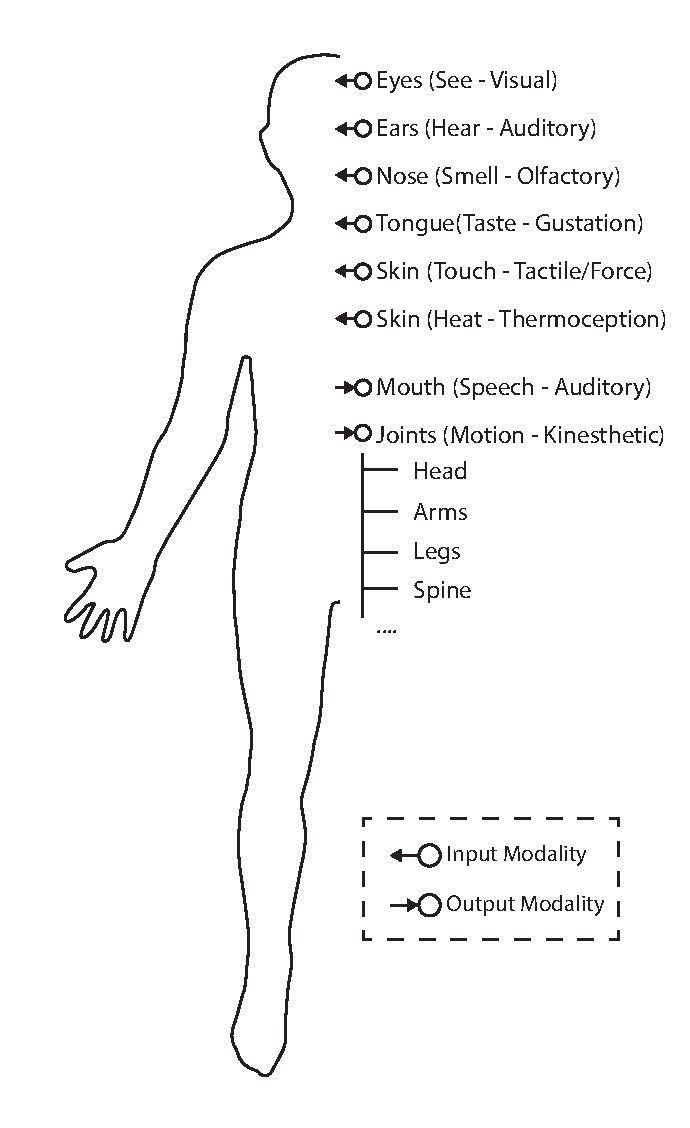
\includegraphics[width=0.6\textwidth]{figures/concept/Modalities.pdf}
\caption{Human Body Schema Input/Output Modalities Map}
  \label{fig:concept-modalities}
\end{figure}

These characteristics help to derive a systematic model of human body schema, in which the structure consists of modularized subcomponents or, as defined herein this thesis, as \textbf{Modalities}. A modality is a single component of body schema that contains an information channel as input or output which interacts with the body representation and surrounding space. \Figure{fig:concept-modalities} highlights the various modalities human body schema can be characterized with. Input modalities refer to the sensory model of human body, and output schema is related to postural model (with an exception to the speech modality).

In order to engineer body schema, and create a transfer model which alter the sense of body representation and how we interact with it, we can decouple the body schema representation into a set of modalities. In this thesis, the process of decoupling is called as ``Loosely-Coupled Modalities''.

\section{Loosely-Coupled Modalities}
\label{sec:concept-LCM}

As in our daily interaction, we rely on cross-modalities to have a clear comprehension of the tasks involved in. Human body physical structure imposes tight coupling of these modalities, and our mental representation is mapped to this tight coupling. Ability to isolate and separate these modalities can help to redesign new sort of perceptual augmentation interactions by modulating the information channels from the representation and feed them back to the human body through perceptual proxy devices (such as HMD, haptic interfaces, ... etc). 

\begin{table}[htp]
\centering
%\hspace*{-1cm}
\centerline{
\begin{tabular}{|l|l|l|l|}
\hline
\footnotesize
\rowcolor[HTML]{EFEFEF}
 \textbf{Modality} & \textbf{Data Representation} & \textbf{Capture Device} &  \textbf{Representation} \\ \hline
\textbf{Vision} & Imagery & Cameras & HMD \\ \hline
\textbf{Hearing} & Auditory & Michrophone & Speaker \\ \hline
\textbf{Speech} & Auditory & Michrophone & Speaker \\ \hline
\textbf{Kinematic} & Spatial & Motion Tracking & Servo Motors  \\ \hline
\textbf{Touch} & Vibratory Signal & Force/Tactile Sensors & Haptic Display \\ \hline
\end{tabular}
}
%\hspace*{-1cm}
\caption{Examples of human body modalities \& corresponding representations }
\label{table:concept-modalities}
\end{table}


The idea of Loosely-Coupled Modalities (LCM) resides on treating each Input/Output modality as a separate channel of interaction. LCM simplifies the body schema structure into primitive modalities, such as joints that can be represented by position and orientation, visual input for each eye, auditory input and output for the ears and the mouth, ...etc. The modalities have a predefined information type that only accepts, for example, the joints only accept spatial information but not an audio signal. \Table{table:concept-modalities} shows various modalities with the corresponding data type which accepts. A channel accessor (symbolized by a circle and an arrow) represents the information flow of the modality. Two types of accessors are defined: input and output. An input accessor directs the information flow from the representation into the body through perceptual proxies, and the output directs the internal state of the body to the representation through tracking and sensing devices. The information flow is defined by a digital form, which is sampled through capture devices, and reproduced through perceptual proxies. \Table{table:concept-modalities} lists the modalities with the corresponding representations and information type that can be used to define them.

In this thesis, the body schema modalities are categorized into two types of modalities: 
\begin{itemize}
\item Postural modalities: focuses on the spatial, three-dimensional attributes related to the body and its representation. Mainly consisting of the joints and shape of the body. 
\item Sensory modalities: contains the various sensory attributes of the human body. 
\end{itemize}

Before describing each set of modalities categorizes, the concept of decoupling and re-coupling of modalities is explained. An abstraction model of the postural and sensory modalities are defined and referred to as Topology models of human body. 

A \textit{Topology} was originally derived in mathematics from the fields of geometry and set theory which defines spatial relationships that connects the matter being studied regardless of the dimensional differences (such as length, scale, ...etc) or descriptive properties (such as color, weight, ..etc). For human bodies, two bodies would have the same topology as long as they have the same number of limbs, eyes, ears, ...etc. If a body has experienced certain deformations (such as a lost limb), then its corresponding postural or sensory topology has also been changed.

\pagebreak
\subsection{Postural Modalities Topology}

In order to create a model defining the body structure, a hierarchical model describing the distribution of the joints in the human body is defined. \Figure{fig:intro-BodyTopology} provides an approximation of the body joints topology. In this model, the following region categories are used:

\begin{figure}[b!]
  \centering
  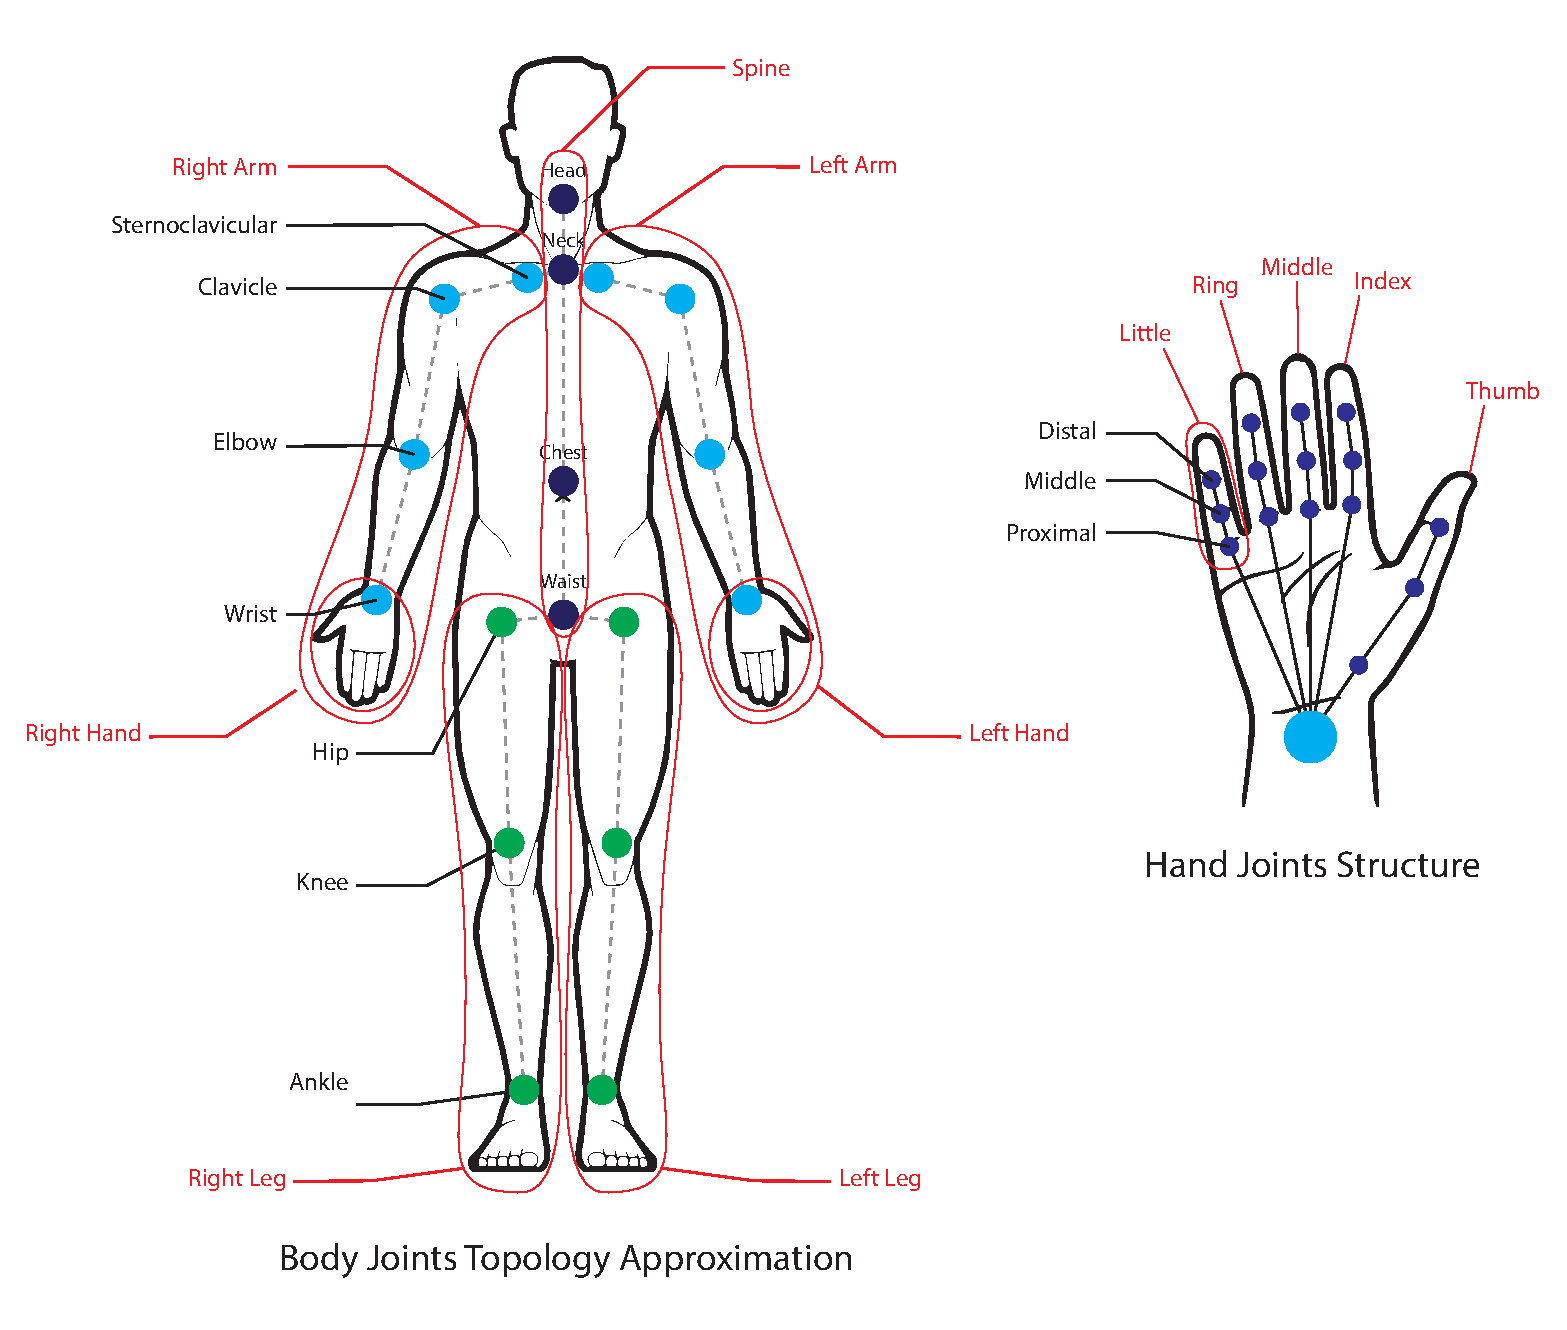
\includegraphics[width=1\linewidth]{figures/concept/BodyTopology.pdf}
  \captionsetup{justification=centering}
  \caption{Body joints topology approximation diagram, and hand joints structure.}
  \label{fig:intro-BodyTopology}
\end{figure}

\begin{itemize}
\item \textbf{Spine Region}: Contains the vertebral column joints which control the overall orientation of the body. The human spine structure consists of 33 vertebrae joints \cite{drakemitchell}, the first 9 joints (from the bottom) are fused into two regions: Coccyx (4 vertebrae), and Sacrum (5 vertebrae). The rest of joints contributes mainly in the motion. Instead of modeling the 24 joints, they were categorized into three regions: Lumbar spine (5 vertebrae) mapped into the Waist, Thoracic spine (12 vertebrae) mapped into the Chest, and Cervical spine (7 vertebrae) mapped into the Neck. Lastly, to provide an individual control to the head, an extra joint to the structure is added as Head.

\item \textbf{Arm Region}: Has the structure of the human arm, and it consists of four joints in total to define the motion of the arm: Sternoclavicular joint, Clavicle joint, Elbow joint, and Wrist joint. The arm also contains a sub-region defining the hand.

\item \textbf{Hand Region}: A sub-region which belongs to the Arm region. Contains the definition of hand joints structure. The hand region is defined by 5 fingers, each finger has the following structure:
\begin{itemize}
  \setlength\itemsep{0em}
\item Proximal Joint: the base joint of the finger.
\item Middle Joint: the second joint of the finger.
\item Distal Joint: tip joint of the finger.
\end{itemize}

\item \textbf{Leg Region}: Defines a general structure of the human leg, and consists of three joints: Hip joint, Knee joint, and Ankle joint.
\end{itemize}


Using the previous categories, it's possible to define a postural body schema as: Spine, Left Arm, Right Arm, Left Leg, and Right Leg. In total, the number of joints defined by this approximation is: 
\begin{equation}
\begin{split}
Joints\ count &=Spine + 2\times (Arm+Hand)+2\times(Leg) \\
&=4 + 2\times(4+15)+2\times3\\
&=48\ joints
\end{split}
\end{equation}

The joint, which is considered as the minimal, atomic representation for postural modality, is defined using two attributes:
\begin{itemize}
  \setlength\itemsep{0em}
\item Position: 3 axis (X,Y,Z) tuple defining joint's spatial position.
\item Orientation: a quaternion defining the direction of the joint. 
\end{itemize}

\pagebreak
\subsection{Sensory Modalities Topology}

\begin{figure}[b!]
  \centering
  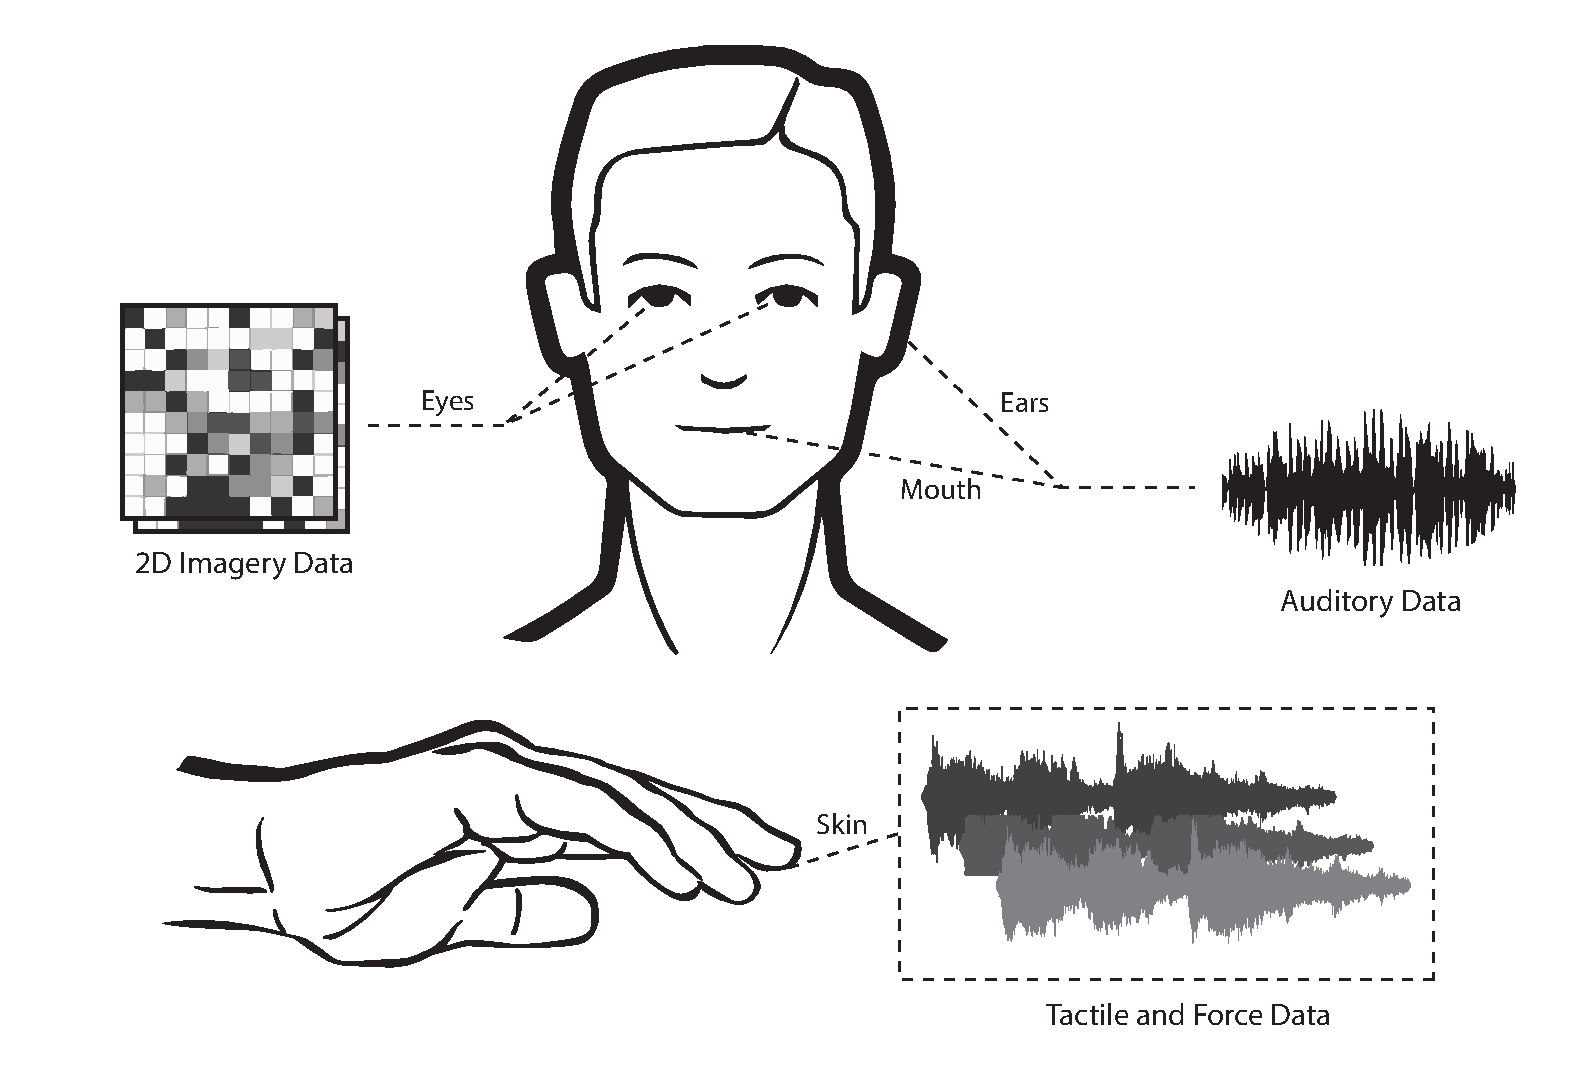
\includegraphics[width=1\linewidth]{figures/concept/PerceptualDataType.pdf}
  \captionsetup{justification=centering}
  \caption{Sensory modalities categorization with their data type.}
  \label{fig:concept-SensoryModalities}
\end{figure}

For the perceptual schema of the body, major sensory modalities are characterized based on their function and data type. \Figure{fig:concept-SensoryModalities} highlights four different types of perceptual modalities with their corresponding data they accept. The sensory modalities considered in this thesis are as follow:

\begin{itemize}
  \setlength\itemsep{0em}
\item \textbf{Eyes}: provide the visual feedback to the user. Consists of two channels: left and right eye. Data type they accept is 2D image data.

\item \textbf{Ears}: provide auditory feedback, and consists of two channels: left and right ear. Corresponding data type is audio signal (sampling rate 44100Hz or higher).

\item \textbf{Mouth}: captures the speech audio of the user. A single data channel with data type of audio signal (sampling rate 44100Hz or higher).

\item \textbf{Skin}: provides tactile and force feedback. Number of channels is defined based on the model (spatial resolution). Accepted data type is a vibrotactile signal.
\end{itemize}

These modules provide the sensory mapping for the human body. The use of digital data as input/output helps to transmit and alter the sensory information using computer mediated communication between the human operator and his representation(s).

\subsection{Decoupling and Re-coupling of Modalities}

In order to simplify the process of modeling the interactions of body schema, the various modalities described previously should use a hierarchical structure to access a region of modalities or the individual atomic level of each sub-modality. 

\begin{wrapfigure}[20]{l}{0.4\textwidth}
  \captionsetup{justification=centering}
  \centering
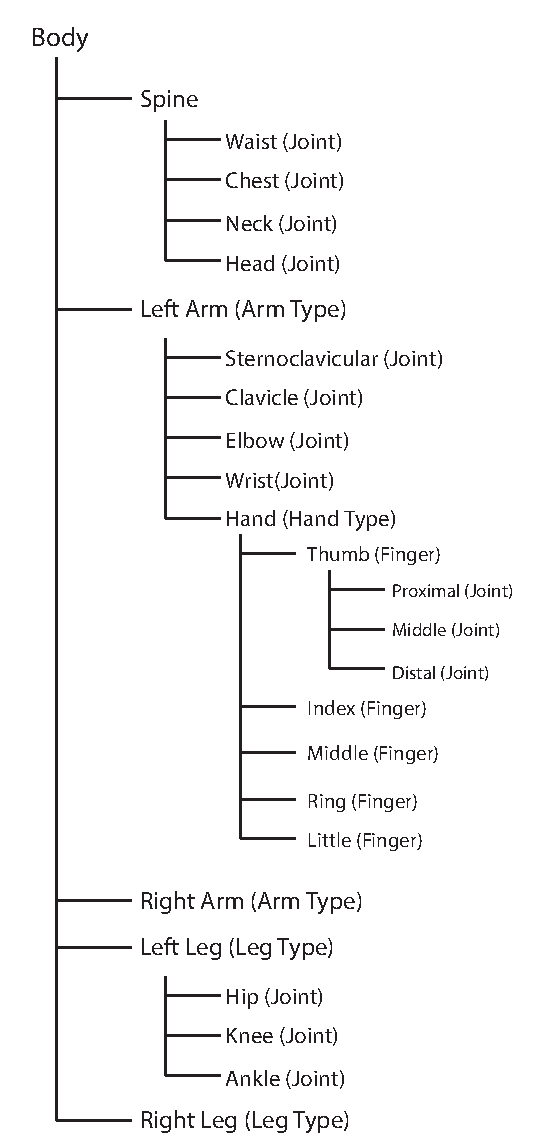
\includegraphics[width=0.4\textwidth]{figures/concept/PosturalSchema.pdf}
\caption{Postural schema hierarchy}
  \label{fig:concept-postural}
\end{wrapfigure}

The use of decoupling/re-coupling in postural schema modeling, it is possible to work at any level of the body structure to map or control the motion of the regions or individual joints \Figure{fig:concept-postural}. For example, its possible to map one arm to another directly, which results to mapping the individual joints of one arm to the corresponding joints of the other joint. Or it is possible to decouple the region into its atomic structure (joints), and reassign them to a different joint, for example controlling the thigh joint using wrist joint. Similarly, for the sensory schema modeling, the stereo eyes can be decoupled into individual left and right eye which are considered the atomic level of visual modalities, and mapped to different sources. The ears can be decoupled to left and right ear, and processed individually.

%\pagebreak
\section{Body Schema Desgin}
\label{sec:concept-bodyschema}

\subsection{Model Oriented}
%express the idea of embodiment using soft representation, and ability to experience it using a physical/virtual representation
%combination of representation and virtual/visual design tools

Embodied Driven Design (EDD) aims to provide a systematic, designer-oriented, human driven body schema design and mapping. By using the idea of loosely-coupled modalities described in the previous section, body schema can be remodeled based on an alternative representation. EDD is based on two design models which defines the target application:
\begin{enumerate}
  	\setlength\itemsep{0em}
\item \textbf{Representation:} The representation of the modalities using physical and virtual means, such as robotic avatar, virtual body, non-humanoid representation, ...etc.
\item \textbf{Meta-Model:} An abstraction of the relationships between the modalities of human body and their corresponding representations. The meta-model defines a transfer function of the schema that can be direct channel mapping, or alternates the information flow of the modalities with their representations.
\end{enumerate}


\begin{figure}[b!]
  \centering
  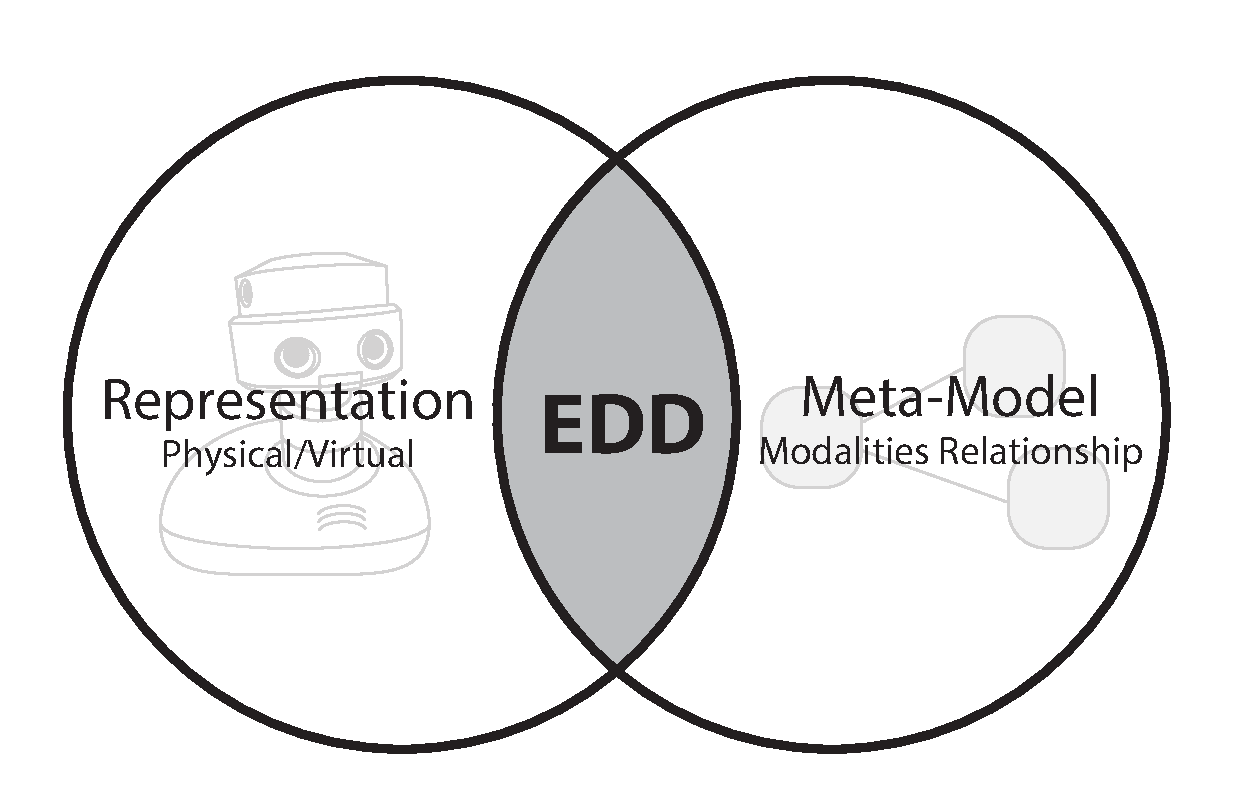
\includegraphics[width=0.8\linewidth]{figures/concept/EDD.pdf}
  \captionsetup{justification=centering}
  \caption{Embodied-Driven Design framework areas.}
  \label{fig:concept-EDD}
\end{figure}


\begin{comment}
\begin{figure}[htpb]
  \centering
  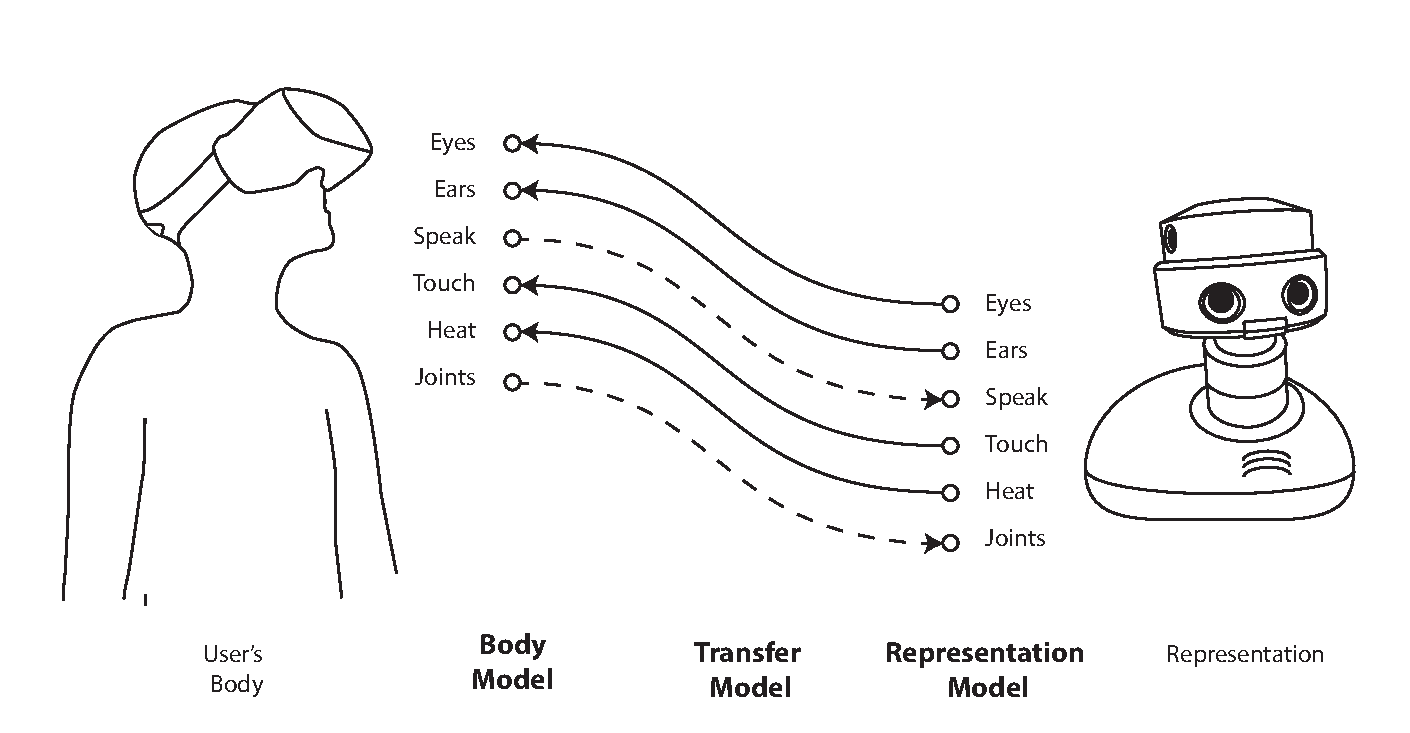
\includegraphics[width=1\linewidth]{figures/concept/EDD-Tx.pdf}
  \captionsetup{justification=centering}
  \caption{An example of EDD for direct one-to-one Telexistence mapping.}
  \label{fig:intro-EDD-TX}
\end{figure} 

\end{comment}


The overlapping of these two regions defines EDD framework \Figure{fig:concept-EDD}. Using such tools of body and representation abstraction, its possible to design new body mapping. A meta-model defines the channel flow between the various modalities that represents the user body in relationship to a representation. As shown in \Figure{fig:concept-EDD-MetaModel}, the meta-model consists of three sets of schematic models:

\begin{itemize}
  \setlength\itemsep{0em}
\item \textbf{Perceptual Model}: provides an abstraction of user's body and reflects its state into the meta-model. Contains blocks that interacts with the user's body modalities via perceptual proxies devices.
\item \textbf{Transfer Model}: an intermediate model residing between the perceptual and representation models. Contains various set of blocks that manipulates the information flow of the used modalities.
\item \textbf{Representation Model}: an abstraction of the representation used (physical or virtual). The blocks contained in this model exchange the information flow from/to the perceptual and transfer models with the used representation. Set of communication channels (e.g. network) exchange the information flow between the model and the actual representation.
\end{itemize}

\begin{figure}[t!]
  \centering
  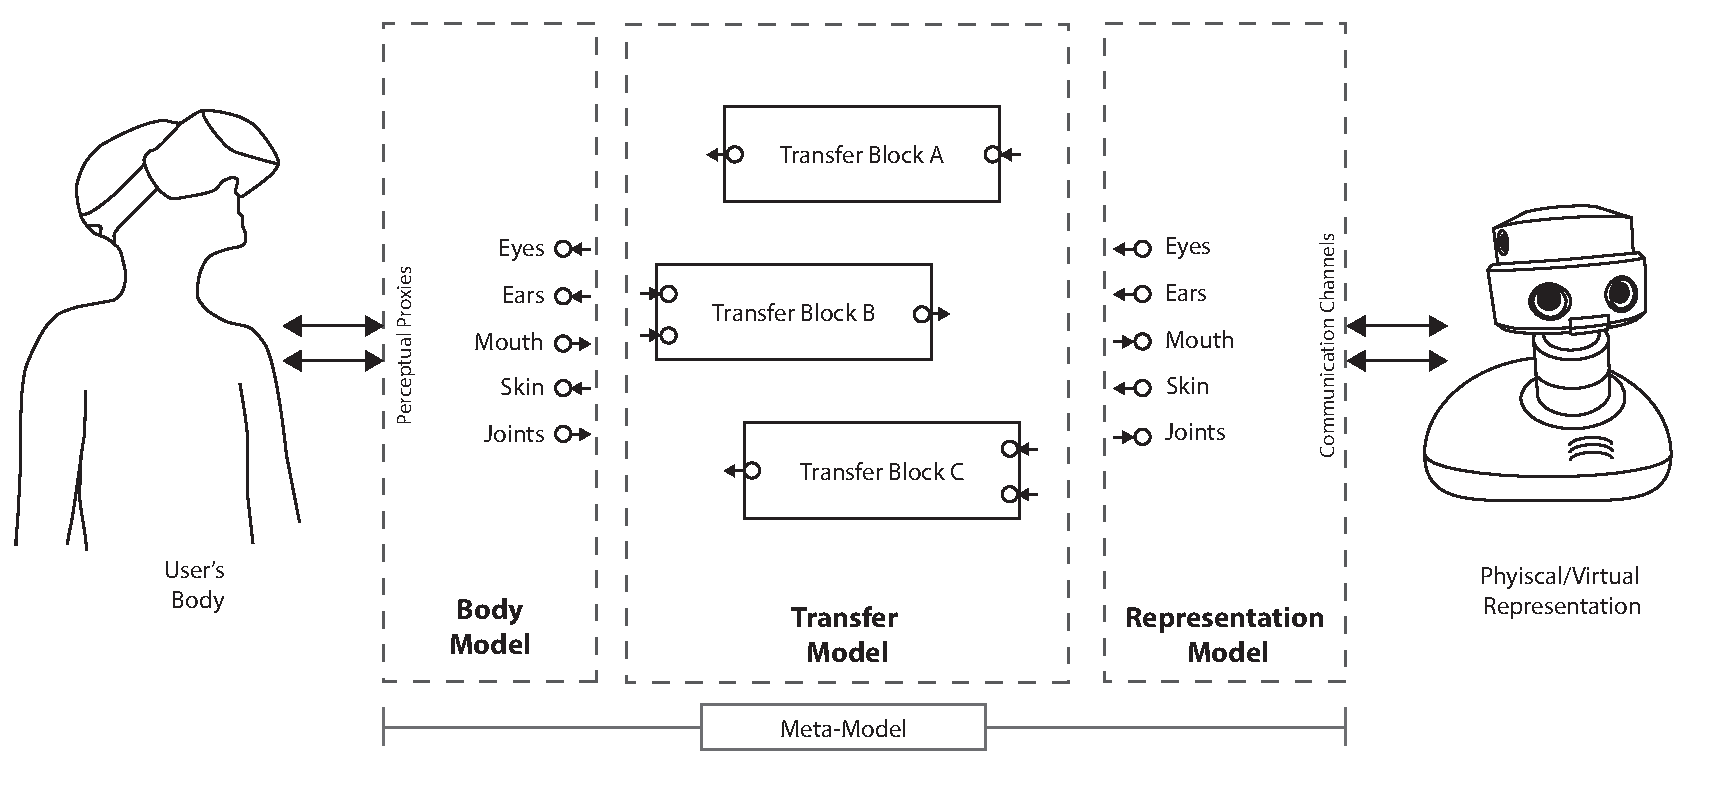
\includegraphics[width=1\linewidth]{figures/concept/EDD-metamodel.pdf}
  \captionsetup{justification=centering}
  \caption{An overview of a general EDD meta-model.}
  \label{fig:concept-EDD-MetaModel}
\end{figure}

Using these three types of models, its possible to define the flow of modalities information of the system. If the transfer model was not used, then a direct schema mapping between user's body and an avatar representation can be defined. As an example of direct schema mapping, Telexistence systems case shown in \Figure{fig:concept-EDD-TX} reflects one-to-one sensory and postural mapping configuration. Since the representation robot offers exact body schema modalities to the user, thus no intermediate transfer blocks are required and the flow between user/representation is direct. 

\begin{figure}[t!]
  \centering
  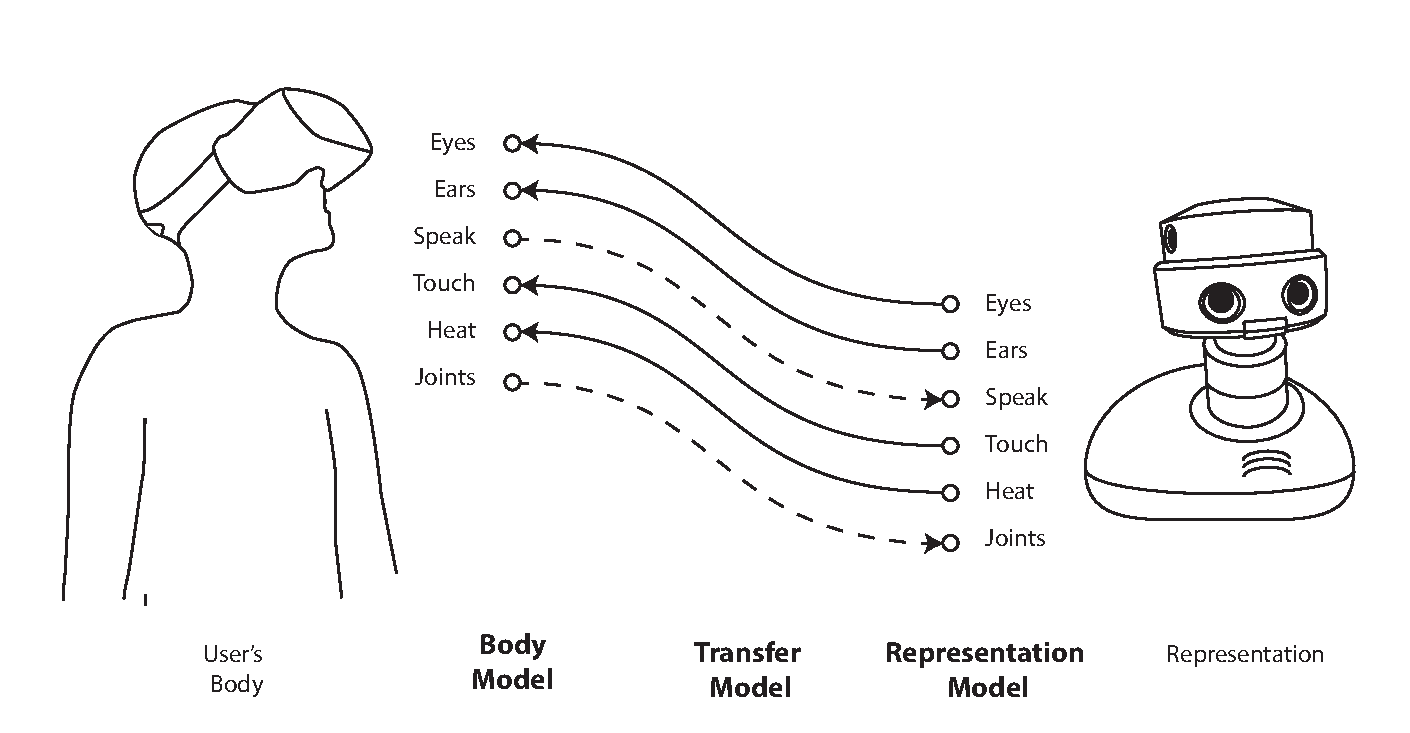
\includegraphics[width=1\linewidth]{figures/concept/EDD-Tx.pdf}
  \captionsetup{justification=centering}
  \caption{An example of EDD for direct one-to-one Telexistence mapping.}
  \label{fig:concept-EDD-TX}
\end{figure} 

%In the following section, further description about meta-modeling design process is described. Before presenting the models, two definitions related to EDD are to be explained: Blocks Categories, and Design Roles.

\subsection{Deriving LCM: Modular Blocks}%Blocks Categories

In order to reflect LCM design pattern of body schema in EDD, each or the three models defines its own set of blocks that handles separate types of modalities and information flow. The following blocks categories define the overall formats that can be used within EDD modeling:

\begin{itemize}
  	\setlength\itemsep{0em}
\item \textbf{Perceptual blocks:} driven from the user postural and sensory modalities such as vision, auditory, tactile, motion, ...etc. Inputs/Outputs of these blocks are used with the perceptual proxy devices (HMD, motion trackers, ...etc). 

\item \textbf{Transfer blocks:} acts as a function for the modalities, in which they transform or alter the data flow between the perceptual and representational blocks. Using these blocks, its possible to alter the limits of certain modalities, augment perceptual modalities, ...etc.

\item \textbf{Representation blocks:} representation dependent blocks, defines the interface and data flow between the used representation (physical, virtual, or both) and the rest of the model.

\end{itemize}


\subsection{EDD Knowledge Areas}
\label{concept:EDDKnowledgeArea}
\begin{figure}[b!]
  \centering
  \captionsetup{justification=centering}
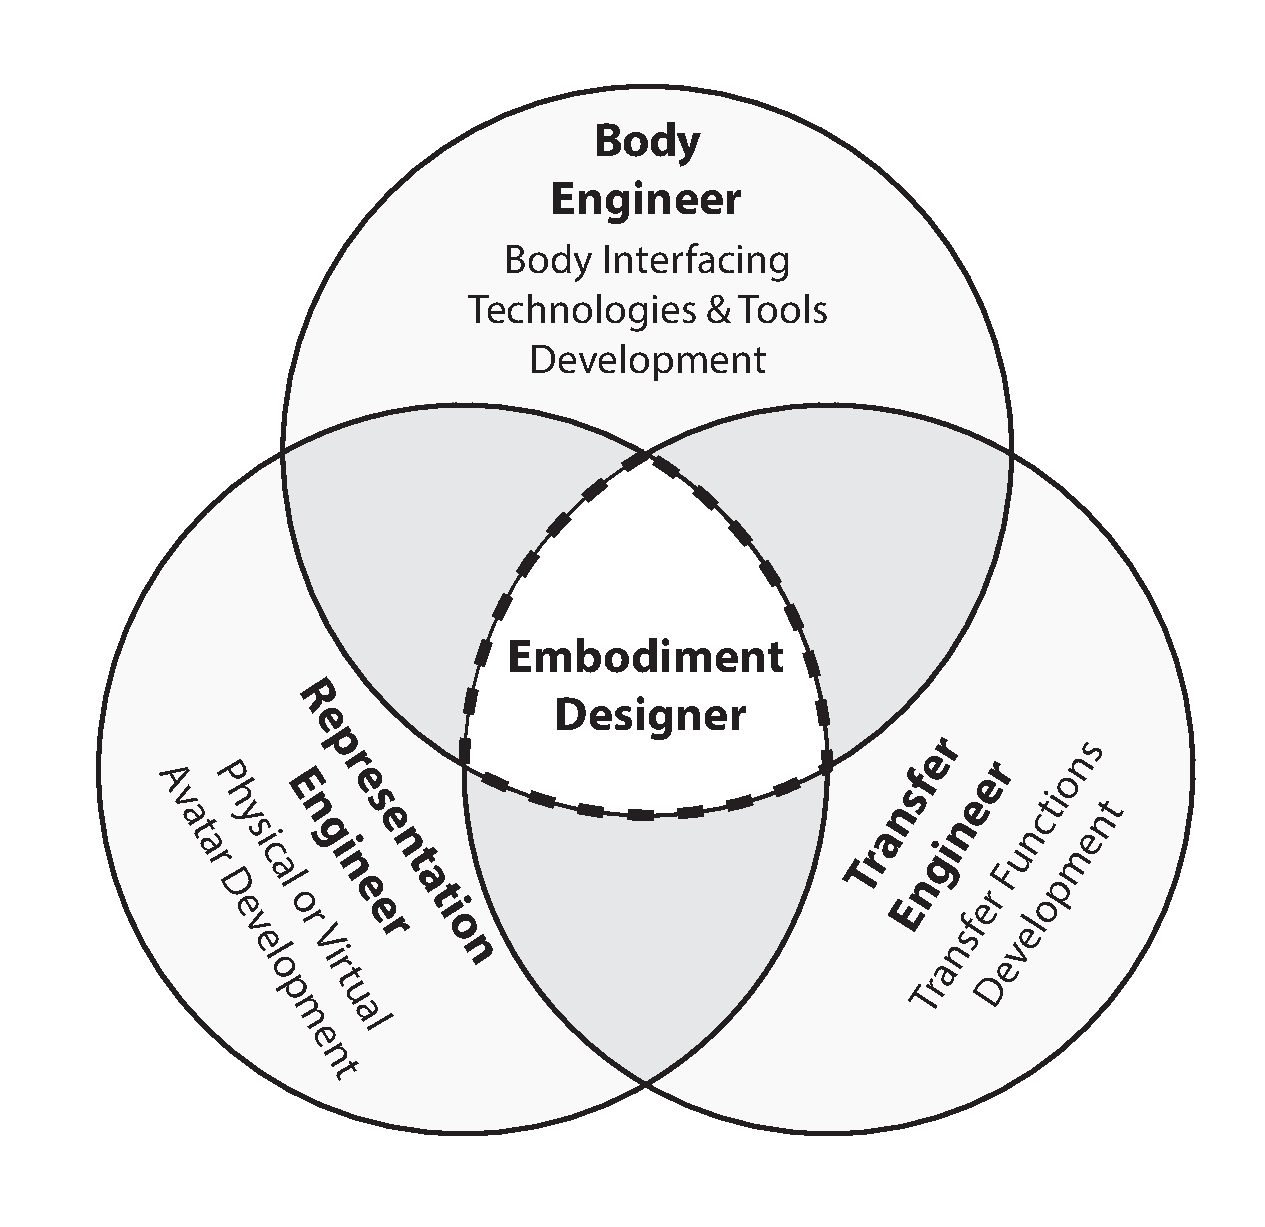
\includegraphics[width=0.6\textwidth]{figures/concept/Roles.pdf}
\caption{EDD Areas of Knowledge}
  \label{fig:concept-roles}
\end{figure}

In this proposal, four areas of knowledge (illustrated in \Figure{fig:concept-roles}) collaboratively contribute to the design process of EDD meta-models, and described as follow:

\begin{itemize}
  	\setlength\itemsep{0em}
\item \textbf{Body Engineer:} a person who uses or develops perceptual proxies and focuses on the experience provided to the user (feedback, tracking method, ..etc). This role is responsible to define and create the perceptual blocks needed in the body model side.

\item   \textbf{Representation Engineer:} this role is responsible on creating the representation blocks used for the target body schema, such as a robotic or virtual representation. 

\item  \textbf{Transfer Engineer:} a role to define and create transfer blocks used to alter the representation or the perceptual blocks. The transfer blocks defined should similar data representation for the other modalities used in the model.

\item  \textbf{Embodiment Designer:} this person creates the overall experience, that is, to use the three types of blocks to define a new body schema. The embodiment designer has an overall knowledge of the perceptual,representation, and transfer blocks to be used. The result is a meta-model designed based on the specific application.
\end{itemize}

In respect of each of the three engineering roles listed above, the meta-modeling process can be more dependent on one role than the other. In the following section, Meta-Models Categories, further description of the use-cases and scenarios in which EDD modeling process contributes into.

%(A), in Another example of EDD for body schema representation is shown in \Figure{fig:intro-EDD-TX} (B), in this case a layered perception module helps to break the one-to-one body constraint mapping to become one-to-many mapping. The module has the responsibility to provide valid perceptual input to the user. 


%\subsection{Sensory Channels Mapping}


\section{Meta-Models Categories}
\label{sec:concept-metalmodel}

Designing a presence or embodied experience requires defining the scope of the application needed, and the corresponding representation and perceptual proxies used. Representation design reflects the modalities which the used representation model affords. The representation exposes these modalities as a set of blocks that can be used in the model. The meta-model defines the connection between these modalities, and user's perceptual modalities through a mediated transfer model. 

Four categories are described here that summarizes the general usability of EDD meta-modeling for overcoming certain physical limitations, or body limitation using a representation. These meta-models describe design patterns for body mapping and configuration, and can be used individually or combined within the same meta-model.

\subsection{Direct Body Transfer}
\label{sec:concept-direct}

In this meta-modeling category, the model directly maps body modalities with the corresponding representation's modalities. \Figure{fig:concept-EDD-Direct} shows an overview of a meta-model mapping. The modalities can be directly connected to the corresponding ones, or can a transfer block could be used to alter the data (for example visual enhancement blocks, audio filter blocks, motion gain blocks, ...etc). This meta-model is generally used for cases in which there is no need to change or alter the topology of the body, and the required application requires minimum adaptation time to the representation. As an example, Telexistence systems use direct body transfer so the user can immediately use the representation (or the avatar).

This meta-model is commonly used along the other meta-models to maintain certain modality mapping without alteration.

\begin{figure}[h!]
  \centering
  \captionsetup{justification=centering}
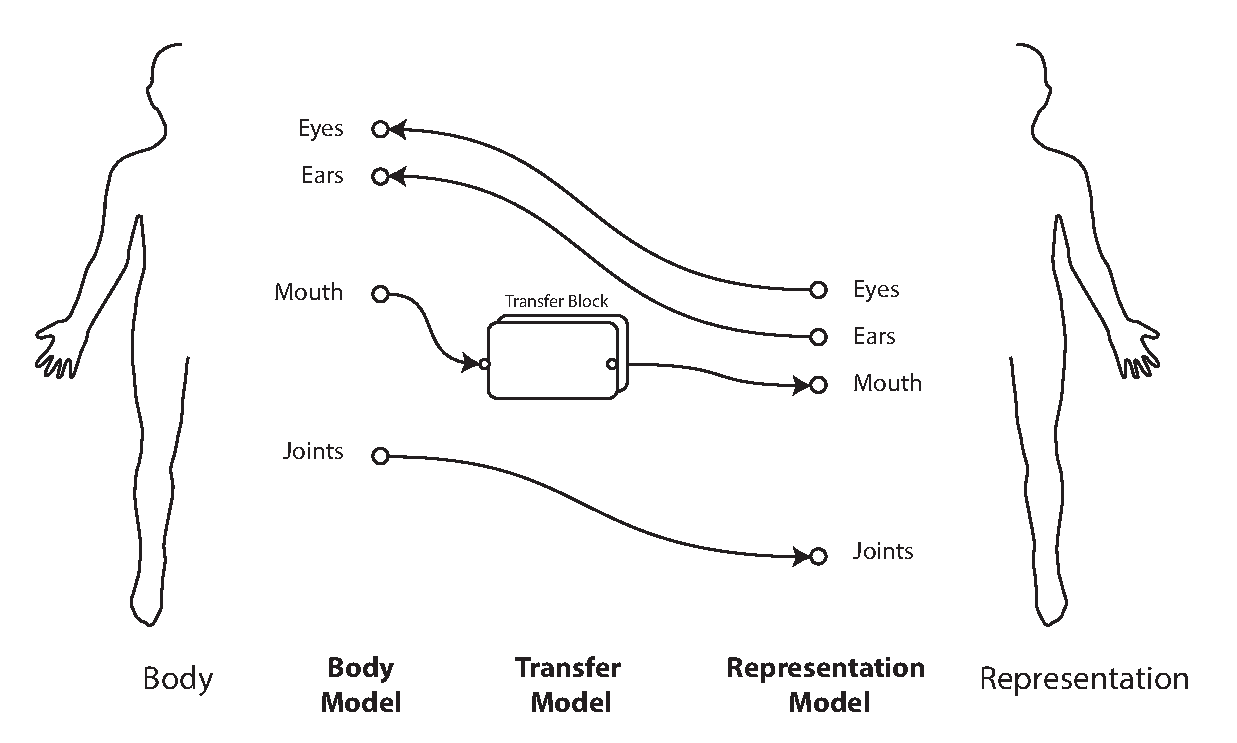
\includegraphics[width=1\textwidth]{figures/concept/EDD-Direct.pdf}
\caption{Direct body transfer meta-modeling.}
  \label{fig:concept-EDD-Direct}
\end{figure}


\subsection{Representation alteration}
\label{sec:concept-RepAlt}


Our bodies are physically limited, and our reaching space is predetermined by the length of the arms for example. Same case is reflected when operating a remote avatar with physical arms, the same physical limitations are presented. In contrast, virtual reality can easily overcome such limitations since objects in these environments are not represented using tangible materials, but instead, a digital body representation can be used.  

Representation alteration design category focuses on redefining the physical representation which can have different properties than what our bodies can provide using a hybrid virtual/physical model of human body. In this design approach, only certain modalities are physically represented (such as vision and auditory modalities) depending on the application, and other modalities are virtually defined. For example, providing a different body visuals or size than the actual. 

\begin{figure}[h!]
  \centering
  \captionsetup{justification=centering}
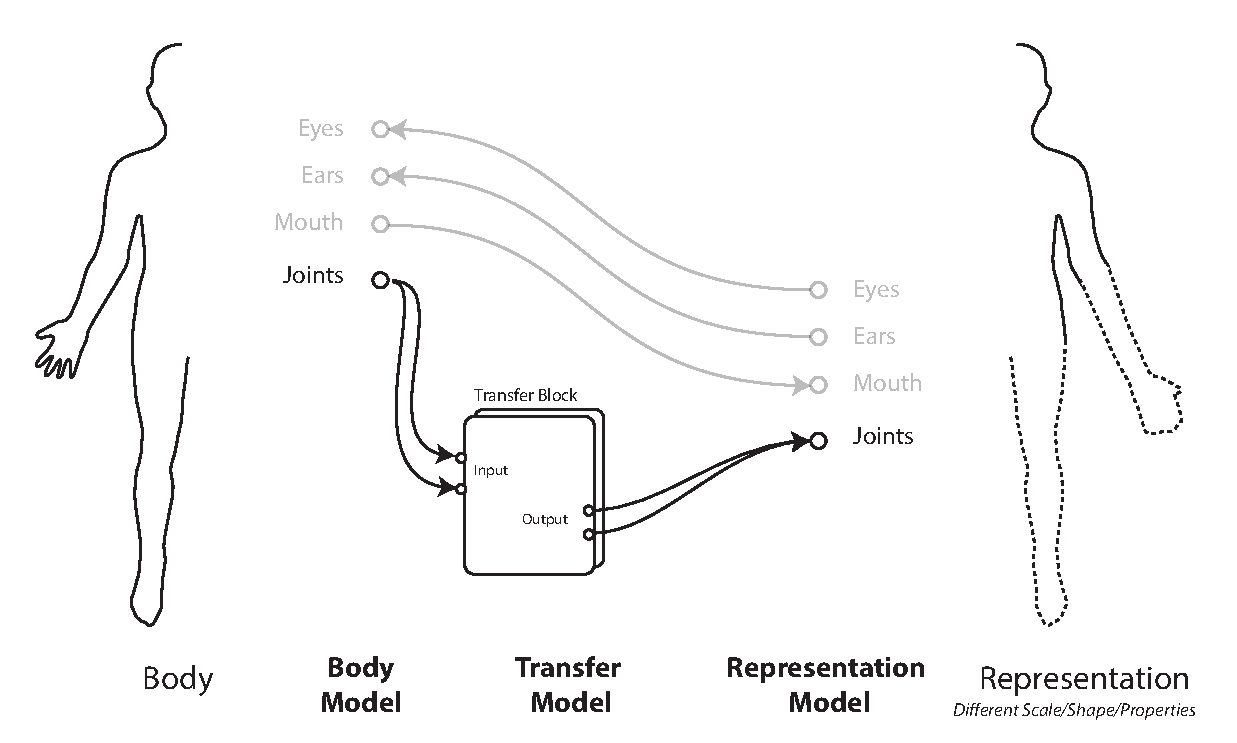
\includegraphics[width=1\textwidth]{figures/concept/EDD-RepAlt.pdf}
\caption{Representation alteration meta-modeling.}
  \label{fig:concept-EDD-RepAlt}
\end{figure}


%In order to maintain natural operation while using representation alteration design, the system should preserve operator's body visual representation both locally and remotely, also to provide mutual presence of user's interaction, the system should also presents operator's body visuals remotely. 


To visualize the representation alteration, \Figure{fig:concept-EDD-RepAlt} shows an overview of this meta-model. The representation has different attributes than the human body has, and can be represented by a hybrid physical/virtual body. For example, the representation can have different arm length than the body has, or dynamically changing its length. The mapping between the body and the representation is altered using transfer blocks that, for example, calculates the required trajectory of the representation body, and maps into the new limbs. Although the body shape changes, its topology is maintained without any alteration.

%To address the previous points, first a hand tracking device is required in order to capture user's hand visuals and motion relatively to his eyes so the eye-to-hand vector can be reconstructed at the robot side (\textit{Perceptual engineer}). Also, the body representation requires to provide visuals of the hands as being projected. To address this, a projector can be embedded into the robot which can reproduce the images of user's hands remotely (\textit{Representation engineer}). The overall system then can be modeled through EDD reflecting the components interacting between the user and the hybrid representation. \Figure{fig:concept-EDD-Mutual} shows the meta-model of this system which combines both transfer and representation blocks. As can be seen, the representation blocks does not directly map into the modalities offered by the user (virtual hands and wheels motion), and some modalities from user's side require transfer blocks to be used in the representation. The virtual hands block requires at the representation side displays user's hands remotely, and thus it requires hands image information. For this, a transfer block is used as [Hand Segmentation]. Also, in this representation, wheels are used for navigation and would require a motion vector to drive. The postural schema is different from user's schema, and thus another transfer block is also required [Motion Control].

%In the user side, the hands are captured using a first point of view (FPV) tracking camera mounted on the front of the HMD. The output of this camera is provided through the [Hands] block which is part of the postural schema of user's body. This block is linked to [Hand Segmentation] block which is responsible to extract hands information. The output of this block is mapped to [Virtual Hands] block which is used by the representation to project hands visuals. For [Motion Control] block, a body as a joystick concept can be used to drive the robot. [Motion Control] block receives head motion, and based on it calculate the motion speed and rotation which is linked to the [Wheels Motion] block to drive the robot's wheels.

In summary of Representation alteration modeling category, the design process for this meta-model is mainly derived from the body limitations. By altering the representation, and reflecting this alteration into a set of meta-modeling blocks, it's possible to match them with the modalities provided by the perceptual model.

\subsection{Topology Reconfiguration}
\label{sec:concept-OpAlt}
% \protect\footnote{Relevant work by the author \cite{saraiji2015hug}}}


\begin{figure}[b!]
  \centering
  \captionsetup{justification=centering}
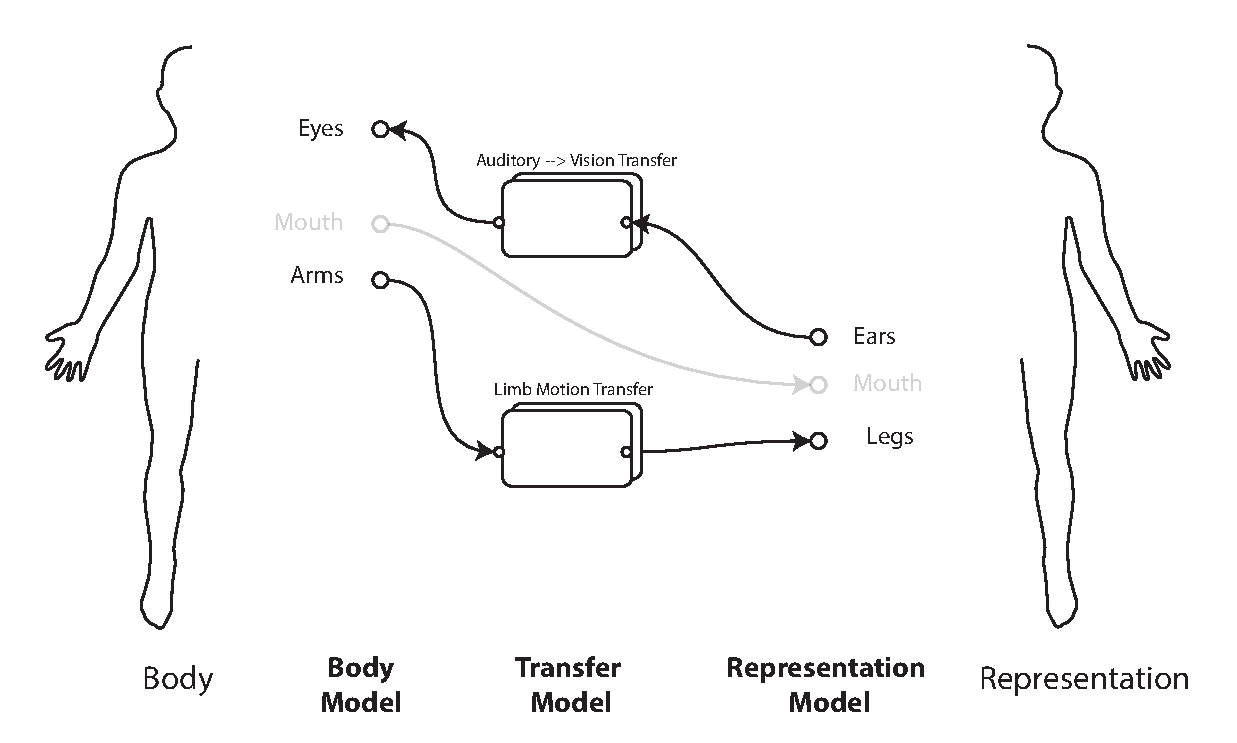
\includegraphics[width=1\textwidth]{figures/concept/EDD-Top.pdf}
\caption{Topology reconfiguration meta-modeling.}
  \label{fig:concept-EDD-TopRec}
\end{figure}

When physical limitation prevents certain modalities to be used, or when a new bodily function that is not driven from the human body in the representation requires matching with operator body, then the design process is focused on the body topology side. Topology Reconfiguration design category focuses on altering the postural modality data flow from the user side and mapping it into the intended representation. This design category can be used to enable physically impaired users or people with lost limbs to alter their body schema and use different functional limb as a substitution for a modality. For example, a mobility impaired person (cannot walk), can use his head motion as an alternative method in order to navigate using the remote representation. This would provide direct and embodied operation, and would require a minimum amount of training to use.

To illustrate this meta-model design pattern, \Figure{fig:concept-EDD-TopRec} shows an example of reconfiguring body topology (postural and sensory topologies) by redirecting the mapping of the body's modalities into different modalities in the representation. To achieve such mapping, transfer blocks are required to translate the information flow between such modalities. For example, sensory substitution can be considered as topology reconfiguration, in which one sensory organ is mapped into another by converting the source information into the target modality. 

There are considerations when topology reconfiguration is intended to be used. Certain modalities should not be arbitrarily mapped to a different one. For example, mapping wrist tilts rotational axis into panning axis of the head motion. This type of modulation would cause disembodiment although the motion is driven by the wrist. To avoid such disembodiment cases, its possible to define set of constraints on the joints channel mapping:
\begin{itemize}
\item \textbf{Rotational mapping}: Joint axes should be mapped as:
\begin{equation}
\begin{split}
DestJ_{tilt} &=F_{A}(SrcJ_{tilt}) \\
DestJ_{pan} &=F_{B}(SrcJ_{pan}) \\
DestJ_{roll} &=F_{C}(SrcJ_{roll})
\end{split}
\end{equation}
$SrcJ $: Source joint (driving joint from the user side).\\
$DestJ$: Destination joint (target joint at the representation side).\\
$F_{A},F_{B},F_{C}$: are functions that can be applied on each individual axis to alter the motion (e.g. linear mapping $F(X)=X$)

\item \textbf{Spatial mapping}: Similarly to rotational mapping constraint, the spatial mapping constraint the mapping between axes (X,Y,Z) to the corresponding ones in the destination.

\item \textbf{Directional mapping}: The spatial and rotational mapping should follow the sign of the source motion (not to use inverse function on the joint motion).

%Side mapping (left--> right) [Need references]
\end{itemize}

In summary, this design pattern is intended to remap body modalities into different ones in order to overcome a physical disability imposed by a certain modality. This design pattern can be combined with other meta-modeling design patterns when designing a system.

%To highlight the meta-model process for topology reconfiguration, a scenario is described here. The representation system used is an ordinary telexistence system as shown in \Figure{fig:concept-EDD-Redirected}. The user side, however, can not use head rotation due to physical limitations, and thus a different postural modality to be used. In this example, the user wants to operate the head motion using his eye gaze motion, so when the user looks left, the robot head starts to pan to the left side, and vise-versa for the right side. Similarly, looking up would tilt the head to up, and vise-versa for the bottom. The motion mapping follows the constraints described previously. For this meta-model, an [Eye Gaze] perceptual block is used to measure the pupil position of the user, and it outputs a 2D vector (X,Y) describing the pupil looking location along the horizontal and vertical axes as value range of [-1,1] for each axis. To translate this vector into a rotational joint output, a [Motion Transfer] block can be used. It converts an input vector into tilt and pan rotation, which then can be linked into a destination joint. The output of [Motion Transfer] block is linked into [Head Rotation] at the representation model.




\subsection{Modality Expansion}
\label{sec:concept-ModAlt}
%\protect\footnote{For further details regarding Layered Presence, please refer to author's papers \cite{saraiji2016layered,saraiji2016study}}}


\begin{figure}[htpb]
  \centering
  \captionsetup{justification=centering}
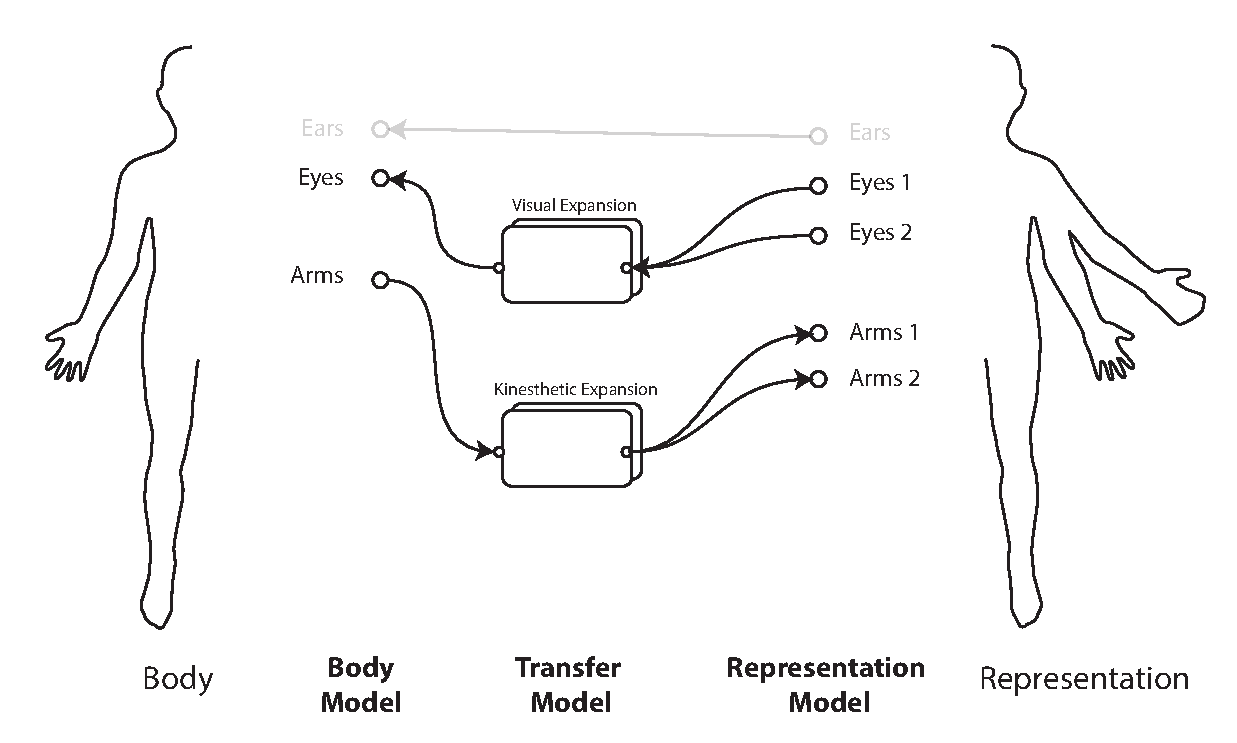
\includegraphics[width=1\textwidth]{figures/concept/EDD-Expansion.pdf}
\caption{Modality expansion meta-modeling.}
  \label{fig:concept-EDD-ModExp}
\end{figure}

The previously proposed design patterns have mainly addressed direct one-to-one body schema mapping in which each body modality communicates with a single modality at a time. In that type of systems, the sensory and postural topologies are constrained to a single representation. \textit{Modality Expansion} design pattern addresses systems with non-linear mapping, that is the operator can access multiple modalities and receives feedback from them, or controls them simultaneously. This control and feedback mechanisms in this meta-model should address the following considerations:
\begin{itemize}
  	\setlength\itemsep{0em}
    \item Real-time simultaneous representation of body, visuals, and auditory feedback in multiple locations.
    \item Natural mechanism of presenting the visuals from the multiple sources to human user.
    \item Intuitive mechanism for switching the visual perception between the locations, while maintaining the awareness of the other locations.  
\end{itemize}

To illustrate this design pattern, \Figure{fig:concept-EDD-ModExp} shows mapping body modalities into multiple modalities in the representation. The representation can be single with multiple modalities, or several representations that the user connects to and controls simultaneously. 

To design a meta-model that can provide such non-linear mapping of body topology and representation topology, the concept of ``Modality Layer'' is used. The layer contains both the postural and perceptual modalities of the representation used, and thus when $N$ modalities are required to interact with, we would have $N$ layers [$L_{1}...L_{N}$] that are derived from these modalities. These layers are aggregated together to produce the input to the perceptual or postural modalities of the user. These layers can be mixed (or blended) and delivered to the user and representation using corresponding transfer blocks.

This design pattern helps to expand body's limitations to perceive and control multiple representations that can be located locally, or connected remotely (ubiquitous).

%This method can be expanded to more than just Telexistence related applications. By using the concept of layering, its possible to generalize the layers to be media or even interactive applications, and apply the same procedure in combining them into a single space. 



\pagebreak

\section{Physical Embodiment Toolkit}
\label{concept:toolkit}
%describe the goal of the embodiment toolkit

In order to facilitate the process of prototyping meta-models and experiment the effect of altering the mapping of various modalities, an embodiment toolkit is proposed. The toolkit is a general purpose physical representation designed in a robotic form, which provides essential modalities to access through EDD framework. This toolkit can be looked as being a tool to reprogram our bodies and our presence. The design considerations for this proposed toolkit are described in this section. 

For this thesis, this toolkit was used completely or partially in several projects (discussed in \Chapter{ch:eval}) and provided an agile design and testing process for these projects.

\subsection{Human Driven Design}

Human bodies provide high degree of complexity and constraints. The toolkit should provide a balance between the complexity of replicating the human body structure and the affordability to create a general purpose system. The following modalities are mainly considered to be available in the design of the hardware:

\begin{itemize}
\item \textbf{Vision feedback}: as in teleoperation and presence applications, the main sensory feedback we would rely on to gather information about the surrounding environment is the vision, or the eyes. The representation should provide means of capturing real-time visuals and provide them in bodily acceptable format, that is a stereo vision. As in Telexistence systems, stereo vision is an important design consideration that is required by the slave system to provide. For general use case purpose, the interpupillary distance (IPD) for the vision system is to be fixed on an average of 64mm \cite{dodgson2004variation}. Field of vision should be wide enough to cover at least $60\deg$ of user's field of view, so the user can obtain feedback from the peripheral vision. The visual feedback should provide real-time feedback with corrected distortion in order to avoid ``Motion Sickness'' cases, that is, the disagreement between visually perceived optical flow and motion, and the vestibular system's sense of movement which caused the motion. In this thesis, the latency considerations should be less than 100ms for the visual system. The responsiveness (or framerate) of the vision system should be high enough to minimize the motion sickness as well as balanced to maintain low latency feedback (the higher the framerate, the more performance demand from the system is required, and thus higher latency will occur). Within these constraints, the spatial resolution of the images can be considered depending on the target application (for teleoperation and inspection purpose, low resolution can be sufficient to be used).

To use in EDD, the toolkit should expose a block that provides access to the eyes modality of the representation. In the representation model category, [Eyes] block is used to output stereo visual data channel from the toolkit into the meta-model.

\item \textbf{Auditory feedback}: The auditory system of human body is an important cue to have spatial awareness of the events occurring around. The binaural feedback provides an understanding of the sound sources locations. For this modality, the system should provide a similar experience of human ears. To maintain high auditory spectrum feedback, the audio system should provide high-frequency sampling of the audio. Human ears can perceive a range of 20Hz to 20,000Hz of auditory spectrum. Thus the sampling rate should be at least twice the frequency (based on Nyquist–Shannon sampling theorem), so 40,000Hz audio sampling is the minimum requirement for the audio system. The closest supported standard audio frequency by the hardware is 44,100Hz. The audio transmission should be synchronized with the visual feedback in order to avoid any disengagement of visual-auditory cross-modality during operation. 

The auditory feedback is integrated into EDD framework by providing [Ears] block under representation model category to output binaural audio data channel from the toolkit into the meta-model. 

\item \textbf{Verbal communication}: Since the representation is generally used as a replication of human body, auditory communication system would be required to provide bi-directional audio from/to the toolkit along with the auditory feedback system. The design verbal communication system has fewer constraints than the previous modalities. Single audio channel output is sufficient to be included in the toolkit design. For frequency considerations, this channel mainly transmits the verbal audio from the human operator, thus the frequency sampling can be less than the auditory feedback channels. Old telecommunication systems (such as the telephone) used 8,000Hz sampling rate, although it was sufficient for human speech however it cannot support sibilance (ess/s/ and eff/f/ sounds ). To overcome this, Wideband frequency 16,000Hz sampling rate is considered for the transmission and playback.

In EDD framework, under representation model category, a [Mouth] block is provided by the toolkit to communicate the auditory data channel from the meta-model to the representation hardware. 

\item \textbf{Postural design}: the mechanical structure of the toolkit reflects the degrees of freedom (DOF) and limits of the operation and mapping with the user. The postural schema of the toolkit should provide visual-kinesthetic cross-modality, thus a structure that mimics the head motion is needed. A three DOF head structure would provide rotational motion along the tilt, pan, and roll axes are sufficient to produce the motion for the eyes. Speed and joints acceleration of the head design is required to match the speed and acceleration of human neck. If an inadequate speed and resolution were used, the system would result in mechanical latency and thus motion sickness would occur. To address these speed limitations, a user-study is required to calculate the maximum rotational speed of human neck. 

For the parallax motion of the upper body, the addition of three extra DOF would provide the lower motion of the human torso \cite{watanabe2008torso}. However, the usage of these extra joints would increase the size and affordability of the toolkit. The addition of these DOFs is optional, and is application specific. Two versions of the toolkit can be designed: Head only (3DOF) and Head+Parallax (6DOF).

The postural modalities are exposed into EDD under representation model category as a set of blocks representing the body. For the neck modality, the [Neck Joint] block is used to communicate the target head orientation and position (if parallax motion was required).

\end{itemize}

\subsection{Extensibility and Modularity}
Although the toolkit provides a minimal amount of modalities as described in the previous point, however, it should also support the ability to modify and extend its functions by integrating new types of modalities into it. A modular design is considered for both the software and the hardware. The design of the software architecture on the toolkit should be capable to handle the addition of new types of functions, while maintaining the existing ones,e.g. adding an extra set of vision module into the toolkit. A common use case for such modularity is the haptic sensors. The number of haptic sensors can vary depending on the application, for example, its possible to integrate a tactile sensor on the bottom of the toolkit to capture the ambient vibrations of the location the toolkit is placed at (table top for example). 

For each of the newly added modules, a separate information channel is generated to communicate with the EDD model. Also, a dedicated block is to be designed and integrated into the representation model (defined by \textit{Representation engineer}).

\subsection{Accessibility}

In order to design remote presence alteration experiences using EDD meta-modeling, the toolkit should provide network accessibility. Thus, all the communications between the toolkit and the user side should be carried over dedicated network channels and in a digitized format. The network medium can be done through wired local area networks (Ethernet), or a wireless medium (e.g. Wi-Fi IEEE 802.11 standard) in cases such as mobility is required. This design consideration helps to allow flexibility in connecting to the toolkit, either as a single toolkit at a time, or multiple toolkits simultaneously. 

\section{Design Summary}

This chapter has introduced the overall concept of Embodied-Driven Design (EDD) and meta-modeling design process. EDD derives the various modalities of the human body in a loosely, hierarchical structure in order to engineer a mapping between a human body and an alternative representation, such as telexistence system. This loosely representation helps to alter the input and output of the modalities, or remap them with non-corresponding modalities at the representation side. Meta-modeling is the process of defining body schema mapping by using various types of perceptual, transfer, and representation blocks. Four meta-modeling design categories were described: Direct body transfer, Representation alteration, Topology reconfiguration, and Modality expansion. These categories provide the design process for the systems that will be discussed in \Chapter{ch:eval}. However, EDD is not limited to these meta-models design categories. To expand the usability and utility of EDD, a physical embodiment toolkit is proposed that it can be used along with modeling framework to achieve customizable body mapping and interaction alterations. This toolkit is also used in the projects discussed within this thesis.




 

\chapter{System Implementation}
\label{ch:impl}

In the previous chapter, the overall design requirements for developing an embodiment and body schema transfer system were specified. This chapter will discuss the implementation details for a designer friendly embodiment modeling framework. The major components for the framework are discussed here: the Meta-modeling editor, modalities information channels and meta-blocks, the integration with an existing game engine (Unity 3D), performance optimizations, and physical embodiment toolkit. 

\section{Embodiment Framework Overview}


\begin{figure}[b!]
\centering
\captionsetup{justification=centering} 
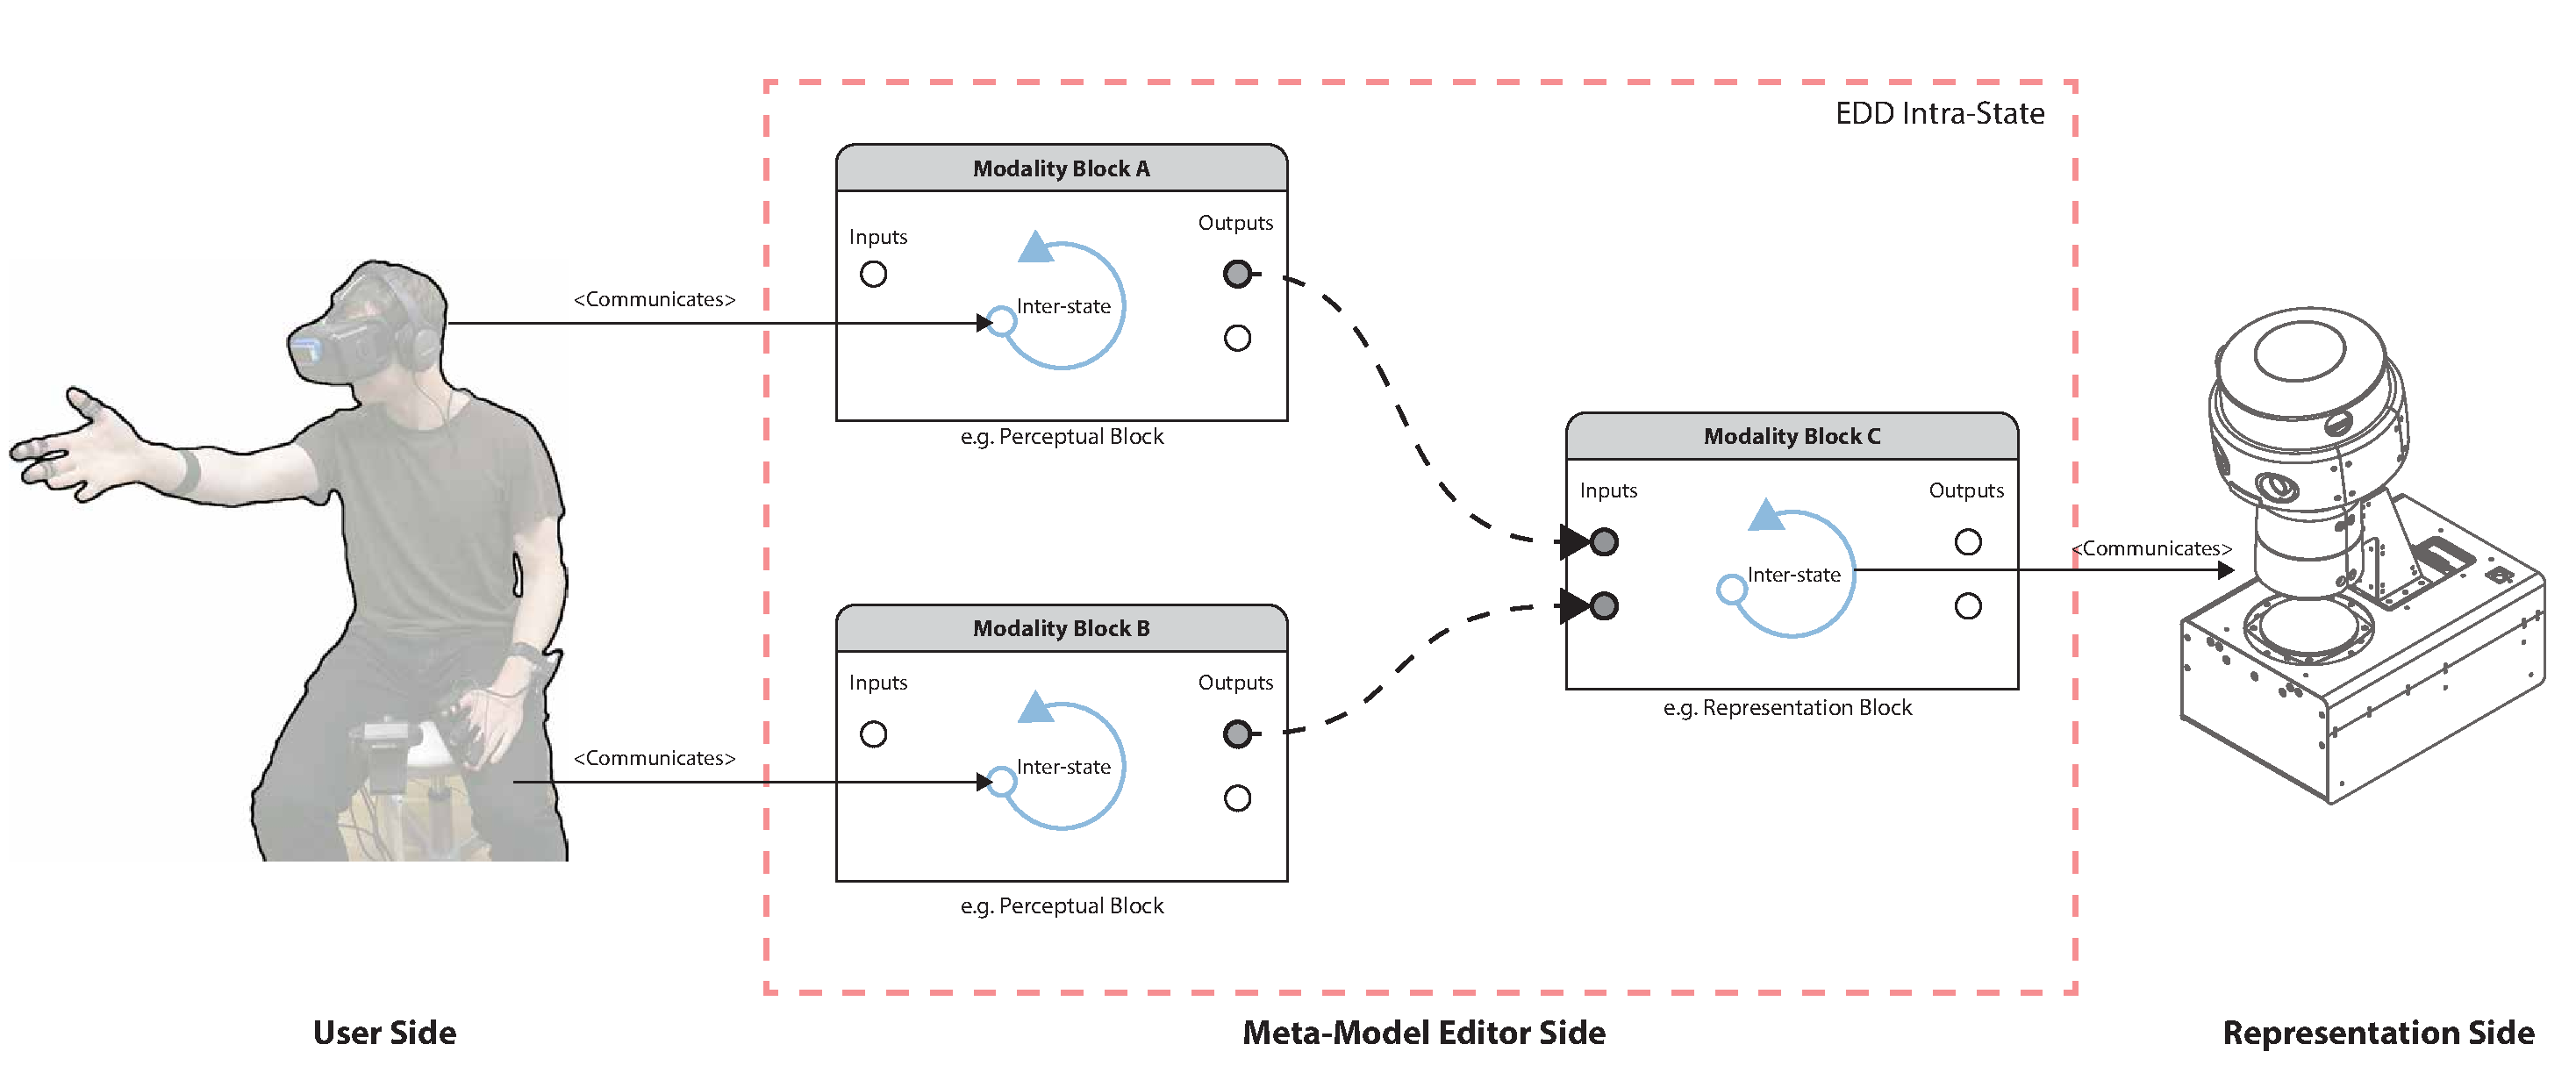
\includegraphics[width=1\textwidth]{figures/system/EDD_Editor_Overview.pdf}
\caption{An overview for Embodiment Framework components.}
  \label{fig:system-edd-overview}
\end{figure}

The embodiment framework contains various components and blocks that defines the topology of the system and representation. An overview of the framework is shown in \Figure{fig:system-edd-overview}. The framework consists of: \textbf{User side} which communicates the state of the operating user with the model using tracking and perceptual devices, \textbf{Meta-Model Editor side} which defines the interacting blocks and modules of the target schema of the system, and \textbf{Representation side} which communicates the state of the used representation (virtual or physical) with the model. 

The user side contains modular tracking and perceptual hardware in which it can be customized depending on the intended application. For visuals presentation to user's eyes, a head mounted display is mainly for presence transfer systems (derived from telexistence systems). For body tracking, several tracking systems has been integrated into the framework in order to assist the degree of body tracking based on the number of joints intended to be tracked. For example, when head tracking is only needed, then HMD built-in tracking functionality can be used without the need for an external tracker, but when eyes, arms or legs tracking was required, then different tracking approaches would be used (individually or combined, e.g. optical tracking and data gloves systems). The perceptual and tracking modalities are exposed into the meta-modeling editor as set of blocks that transfer the state of the modalities from/to the model. For example, a [HMD] block would have an input representing the images to be displayed, and an output for its spatial position and rotation. 

Representaiton side is dependant on the type of the body used in the representation. Two types of representations are addressed: Robotic representation, and virtual bodies. These representations can be used individually or in a combination, for example superimposing virtual arms on the visual feed from a remote robot representation. The representation blocks are responsible to communicate with the used body to transfer the modalities data channels from the meta-model and the representation. For postural modalities, joints data are used to control the position and orientation of the links used in the body (e.g. servo motor for robotic form). Similarly, sensory modalities uses transfer blocks to communicate the captured information flow from the representation to the meta-model. [Eyes] transfer block, for example, provides an image stream from the cameras used in the representation.


The meta-modeling editor handles the inter-states and intra-state of the modalities channels flow of the blocks used. The inter-state corresponds to the internal processes of the block throughout a procedure of capturing the inputs through the available slots, applying internal calculations or alteration to that input channels, and expose the results though output slots with a corresponding data type. The intra-state of the meta-model controls the flow of the channels, and constraints the data flow and types used. The intra-state is defined by the embodiment designer.


\section{Meta-Modeling Editor}

\begin{figure}[b!]
\centering
\captionsetup{justification=centering} 
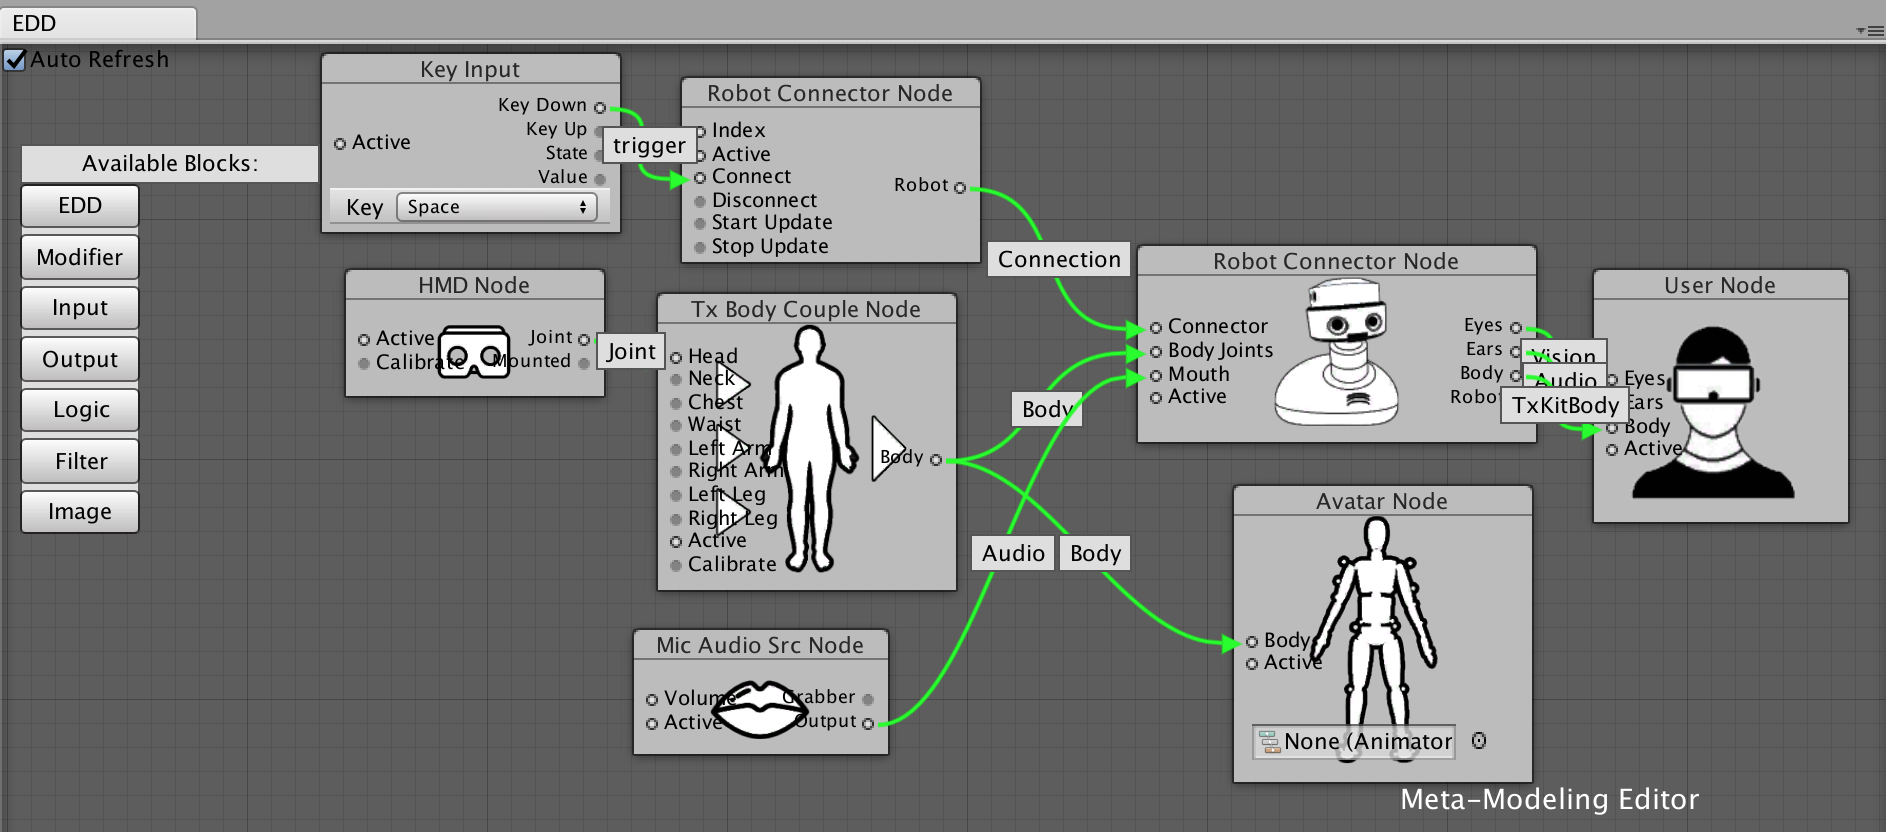
\includegraphics[width=1\textwidth]{figures/system/MetaEditor.png}
\caption{Meta-Modeling Editor Overview.}
  \label{fig:system-metaeditor}
\end{figure}

The meta-modeling editor provides a designer oriented approach to model the interactions between the user and the representation by using various types of meta-blocks. \Figure{fig:system-metaeditor} shows an overview of the meta-modeling editor developed in this thesis. This editor has been implemented under Unity3D. The reason of choosing this game engine in particular is that this engine has been widely accepted platform by both inexperienced and professional designers and programmers, also this engine supports cross-platform deployment which would increase the usability of the meta-modeler system. The design consideration for this editor is to focus on graphically oriented visual programming with minimum amount of writing code to create the model. The editor contains several categories of meta-blocks which can be basic arithmetic or geometric operation blocks, or higher level of interaction such as body tracking blocks. \Figure{fig:system-blocks-nodes} shows how the meta-blocks are organized in a tree structure based on the category and functionality. The designer can access the blocks directly from the side panel in a hierarchical structure, or directly search for the required block by using the search function (Ctrl+Mouse Click) and entering part of the block name in the search box. Using this mechanism, the designer would avoids the confusion of finding the required block. 

\begin{figure}[htpb]
\centering
\captionsetup{justification=centering} 
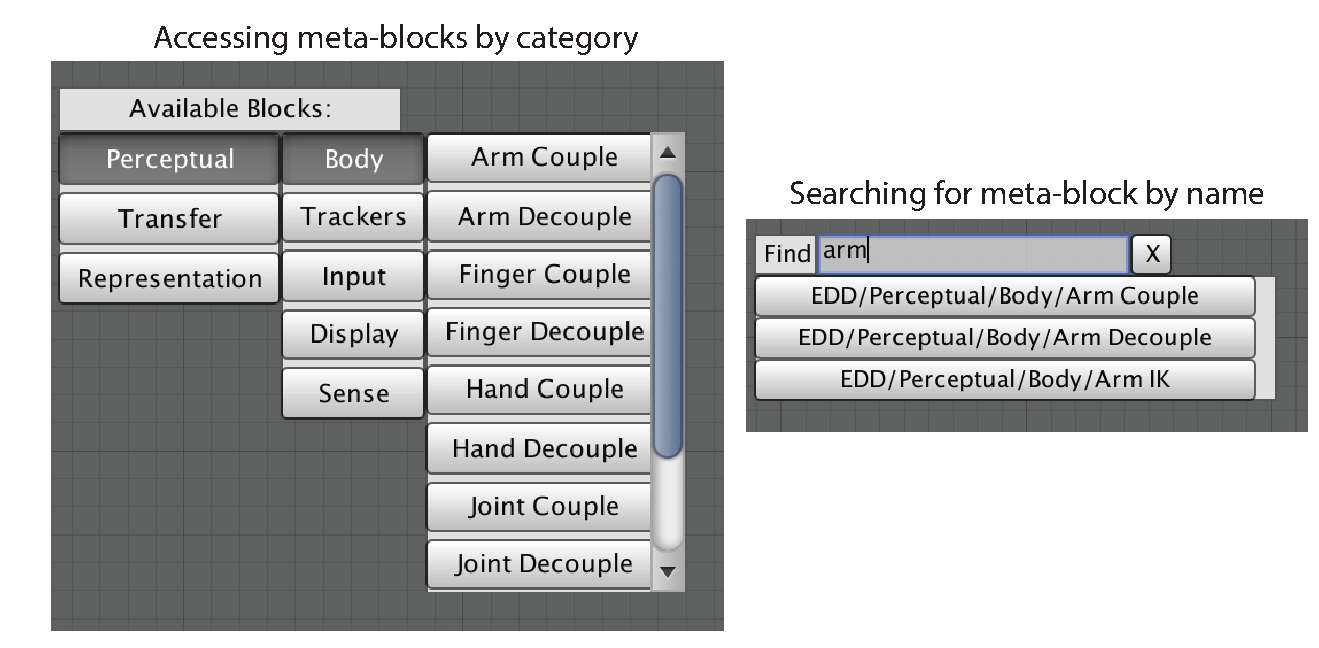
\includegraphics[width=0.8\textwidth]{figures/system/Blocks/Nodes.pdf}
\caption{Accessing meta-blocks by Searching or Category.}
  \label{fig:system-blocks-nodes}
\end{figure}

In order to use the meta-modeling editor, the designer needs to create a new [EDD Model] object under Unity3D editor by choosing: \textit{GameObject Menu \textrightarrow EDD Model}. Once an EDD Model is added, its possible to access the Meta-Modeling editor by selecting the model and clicking [Open Model] from the inspector. The Mea-Modeling editor supports to run multiple models on parallel, so its possible to design dedicate each model into different application or use case. For example one meta-model handles the auditory transmission and alteration, and another one for the body control and mapping. Thus the design process can be distributed.

When a meta-block is added to the model, the block exposes the available input and output channels (or slots) that provides the accessibility from/to its functionality. As a matter of making a convention, the data flow of the blocks always goes from left to right, so input slots are located on the left side, and output slots on the right. When more than one block is added to the model, its possible to connect their channels as long as the channel data matches. Although it constraints the modeling process, however it assists the designer to quickly understand which channels can be connected by highlighting the acceptable input channels in all the blocks added to the model. When channels are connected, a data flow is registered between them. \Figure{fig:system-blocks-flow} shows an example of connecting [Mouth] block into a [Telexistence Robot] representation block. All blocks in the meta-editor contains \textit{Active} state in the input which accepts boolean values, simply used to enable or disable block functionality.

\begin{figure}[t!]
\centering
\captionsetup{justification=centering} 
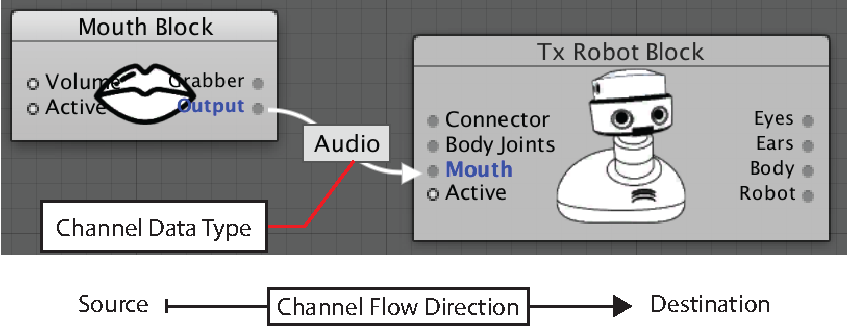
\includegraphics[width=0.8\textwidth]{figures/system/Blocks/Flow.pdf}
\caption{Channel data flow between the blocks.}
  \label{fig:system-blocks-flow}
\end{figure}


\section{Meta-Modeling: Blocks Implementation}

As was described in the design chapter, EDD consists mainly of three set of blocks that can be used to define the body schema transfer model. The design considerations were reflected in the implementation following the same categories for creating meta-blocks. This section describes the details of each block category with the underlying details of the mechanism used in the inter-state of the blocks. 

In order to organize the accessibility to the blocks, each block should define a path in form of ``[Category Name]/[Sub-path]/[Block Name]''. This path is set when the block is implemented in the script. \Listing{lst:blockcode} provides a sample template to declare new meta-blocks. The block class require an attribute of type [ModelBlock] in order to automatically register the block into the graph using the path specified in its argument. Two optional arguments can be added for the icon image and width of the block in pixels in the editor.

\begin{lstlisting}[caption=a definition template class for meta-blocks objects, label=lst:blockcode]
//mandatory attribute, declare this object as being a block in the editor using the specified path, and set an icon image with width of 100px
[ModelBlock("Transfer/Modifier/Block Sample","Icon",100)] 
//the block should be derived from BlockBase class
public class BlockSample : BlockBase 
{
    //internal state variables
    //.....
    //Declare an input channel with data type of XDataType
	[Inlet]
	public XDataType Input{
		set {
		//set internal variables
		}
	}
	//internal block data used for output channel
	YData _outputData;
	//declare an output channel. 
	[SerializeField, Outlet]YEvent OutputY; 
	void Start () {
	    // Initialize block state
	}
	// UpdateState is periodically
	void UpdateState () {
	    //process the internal state of the block
	    //.....
	    //signal outputs
	    OutputY.Invoke(_outputData);
	}
}
\end{lstlisting}


\subsection{Perceptual Blocks Category-set}

This category of blocks are mainly concerned with the user side. The blocks provides a representation of the operator body's state and posture by using \textbf{body state blocks}, which is captured using \textbf{body tracking blocks} , as well as providing to the user information and sensory feedback using  \textbf{feedback blocks}.

\subsubsection{Body State Blocks}

\begin{figure}[b!]
\centering
\captionsetup{justification=centering} 
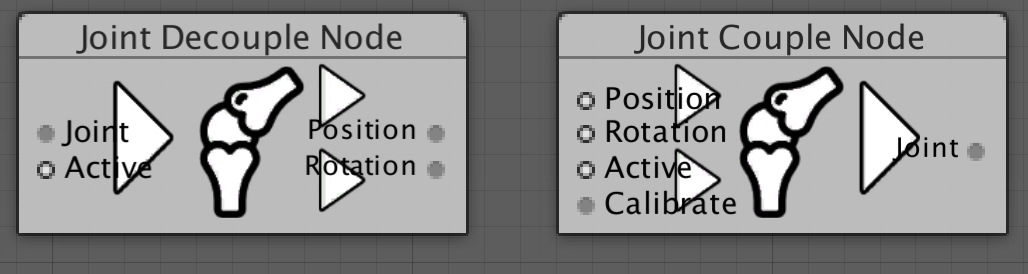
\includegraphics[width=0.8\textwidth]{figures/system/Blocks/Joint.png}
\caption{Joint block, the minimal level of postural schema.}
  \label{fig:system-blocks-joint}
\end{figure}
Body postural representation is designed as a set of blocks that contains the individual joints state. The structure of the blocks follows the previously described Loosely Coupled Modalities (LCM) design pattern in which the structure can be decoupled into smaller regions or grouped back to reconstruct the original region. The minimal region that body structure can be decoupled into is a [Joint] block \Figure{fig:system-blocks-joint}. The joint block contains the spatial attributes represented by a position and rotation channels, which can be captured using [Joint Decouple] block. The position channel accepts a data type of \textit{Vector3} and the rotation accepts \textit{Quaternion} data type. The coordinate system which the joints are represented with is Left-Handed system. Using a singular coordinate system among the spatial blocks is important to decide, so the tracking and representation blocks can use the same system to provide or read the joints data from.

Each joint contains a \textit{Calibrate} input which, when it is triggered, would set the current spatial state of the joint as its initial postural. That is:

\begin{equation}
\begin{split}
Position_{Initial}&=Position\\
Rotation_{Initial}&=Rotation^{-1}\\
\end{split}
\end{equation}
And for each new input value:
\begin{equation}
\begin{split}
Position&=-Position_{Initial}+Position_{Input}\\
Rotation&=Rotation_{Initial}^{-1}\times Rotation_{Input}
\end{split}
\end{equation}

\begin{figure}[b!]
\centering
\captionsetup{justification=centering} 
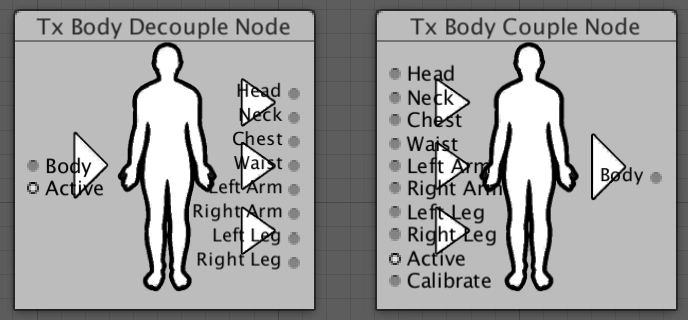
\includegraphics[width=0.8\textwidth]{figures/system/Blocks/Body.png}
\caption{Body decoupling and coupling blocks.}
  \label{fig:system-blocks-body}
\end{figure}

The entire body structure is represented using Body block \Figure{fig:system-blocks-body} which contains a hierarchical structure of the main joints of the spine (waist, chest, neck, and head), two arms and two legs (Left and Right). The body block follows LCM design pattern in which it can supports the decoupling and re-coupling of its sub-structure. Arm block structure is shown in \Figure{fig:system-blocks-arm}. The arm block can be decoupled into four joints (shoulder, clavicle, elbow, and wrist), and a hand. The hand block is structured using five fingers, and each finger has three joints. Finally the leg block is shown in \Figure{fig:system-blocks-leg} and can be decoupled into three joints (hips, knee, and foot). 


\begin{figure}[htpb]
\centering
\captionsetup{justification=centering} 
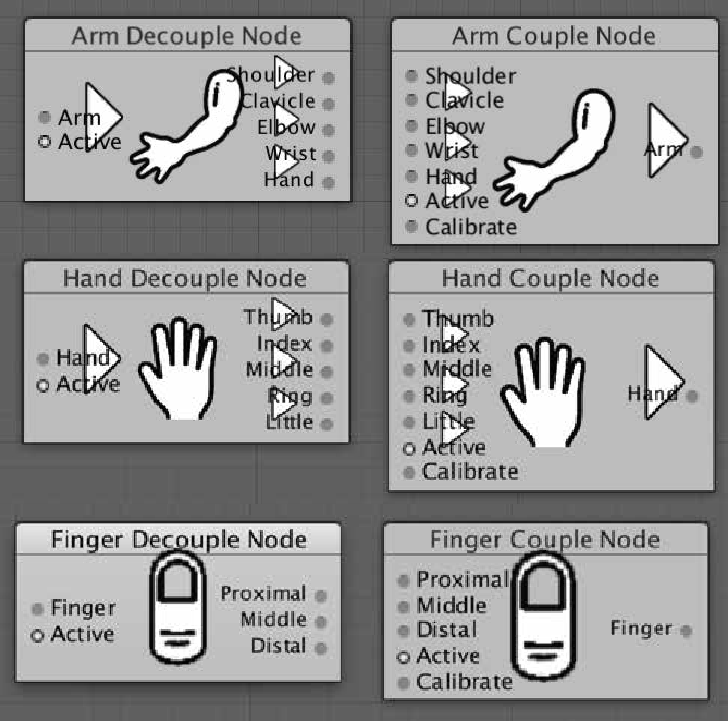
\includegraphics[width=0.8\textwidth]{figures/system/Blocks/Arm.pdf}
\caption{Arm, Hand, and Finger decoupling and coupling blocks.}
  \label{fig:system-blocks-arm}
\end{figure}

\begin{figure}[htpb]
\centering
\captionsetup{justification=centering} 
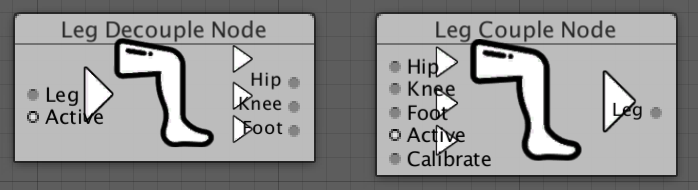
\includegraphics[width=0.8\textwidth]{figures/system/Blocks/Leg.png}
\caption{Leg decoupling and coupling blocks.}
  \label{fig:system-blocks-leg}
\end{figure}

To clarify the benefits of using such highly hierarchical body structure, \Figure{fig:system-bodycoupling} shows an example of how the body parts can be selectively controlled, mapped, and structured. This example shows a single joint controlling two different joints at different levels (head and left arm elbow), while the leg block is mapped into both left and right legs of the body block. Similarly, a single finger block is used to drive three different fingers of the left hand (thumb, index, and little fingers). The data flow type is highlighted on the channels outputs of the blocks. 

\begin{figure}[htpb]
\centering
\captionsetup{justification=centering} 
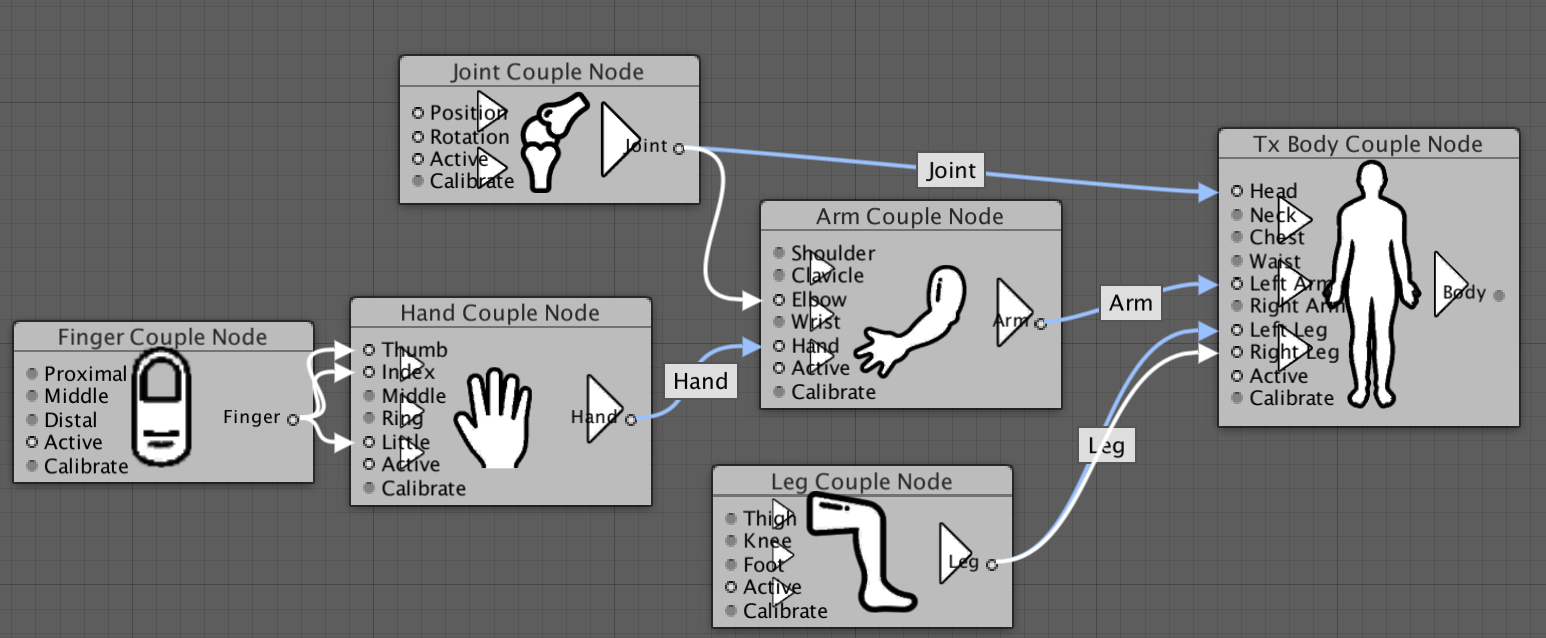
\includegraphics[width=1\textwidth]{figures/system/Blocks/CouplingBody.png}
\caption{An example of Loosely-Coupled Modalities (LCM) to Restructure Postural Schema of the Body.}
  \label{fig:system-bodycoupling}
\end{figure}

\subsubsection{Body Tracking Blocks}
%eyegaze
%body tracking
%hand tracking


For body spatial tracking, various technologies and systems has been tested and integrated into the meta-modeling editor. Each tracking system provides advantages and use cases which varies its functionality from the other systems. \Table{table:system-trackingsystems} summarizes a comparisons between the used systems in term of target body regions required to be tracked (usability), the degree of complexity the system would require to setup and use, and finally the accuracy and robustness of the tracking. Within the tested systems, a trade off between the three criteria was required when deciding the target system to be used in the model. Each of these systems uses different method and procedure for motion capture, and each has its advantages and disadvantages which would constraint the design of the system. In the listed systems, two distinct categories of tracking mechanism are used:


\begin{table}[t!]
\footnotesize
\centerline{
\begin{tabular}{|l|l|l|l|l|l|l|l|}
\hline
\rowcolor[HTML]{EFEFEF} 
\multicolumn{1}{|c|}{\cellcolor[HTML]{EFEFEF}}                                  & \multicolumn{5}{c|}{\cellcolor[HTML]{EFEFEF}Usability} & \cellcolor[HTML]{EFEFEF}                             & \cellcolor[HTML]{EFEFEF}                             \\ \cline{2-6}
\rowcolor[HTML]{C0C0C0} 
\multicolumn{1}{|c|}{\multirow{-2}{*}{\cellcolor[HTML]{EFEFEF}Tracking System}}  & Head   & Hands   & Fingers   & Body   & General   & \multirow{-2}{*}{\cellcolor[HTML]{EFEFEF}Complexity} & \multirow{-2}{*}{\cellcolor[HTML]{EFEFEF}Robustness} \\ \hline
\cellcolor[HTML]{EFEFEF}Oculus HMD                                            & $\surd$    & $\times$    & $\times$      & $\times$        & $\times$      & Low                                                  & High                                                 \\ \hline
\cellcolor[HTML]{EFEFEF}Oculus Touch                                      & $\times$   & $\surd$     & $\triangle$       & $\times$        & $\times$      & Medium$^{1}$                                                  & High                                                 \\ \hline
\cellcolor[HTML]{EFEFEF}Leapmotion                                              & $\times$   & $\surd$     & $\surd$       & $\times$        & $\times$      & Low                                                  & Medium                                               \\ \hline
\cellcolor[HTML]{EFEFEF}5DT Data Glove                                          & $\times$   & $\surd$     & $\surd$       & $\times$        & $\times$      & Low                                                  & High                                                 \\ \hline
\cellcolor[HTML]{EFEFEF}Neuron Perception                                       & $\surd$    & $\surd$     & $\triangle$   & $\surd$         & $\times$      & Medium                                               & Medium                                               \\ \hline
\cellcolor[HTML]{EFEFEF}OptiTrack                                  & $\surd$    & $\surd$     & $\times$      & $\surd$         & $\surd$       & High                                                 & High                                                 \\ \hline
\end{tabular}
}
\begin{tablenotes}
$^{1}$ Oculus Touch require the user to hold them while operation, which is not a seamless tracking method.
\end{tablenotes}
\centering
\captionsetup{justification=centering} 
\caption{A comparison between body tracking systems based on the usability, complexity, and robustness.}
\label{table:system-trackingsystems}
\end{table}


\begin{enumerate}
\item \textbf{Optical tracking}: In this category, the motion capture system uses a single or several cameras (or light sensors) to triangulate the 3D position of a set of points defining the tracked object. Based on this triangulation process, the points are matched with a predefined model representing the tracked object, and then the position and orientation of the object can be calculated. These systems require a calibration process for the cameras to extract the intrinsic parameters (related to the lens of the camera, sensor size, ...etc), and extrinsic parameters (related to the spatial distribution of the cameras when multiple were used, and the location and orientation of the reference ground plane). Since a continuous visibility of the points by the tracking cameras is required, these systems deliver poor tracking when the points were occluded. \\
Two types of tracking systems uses optical tracking:

\begin{itemize}
\item Active type: the tracked points of this system have an illuminating light source (usually within the infrared spectrum) that can be distinguishably tracked from other non relevant points in the environment. Both Oculus HMD and Oculus Touch uses this mechanism for tracking.

\item Passive type: in this type of systems, the tracking cameras are equipped with a special light source (usually infrared light source) that illuminate the environment. The markers or features that needed to be tracked usually reflect the illuminated light back to the camera (usually using a retroreflective material), and thus can be extracted. In this type of systems, usually high noise occur and would require tuning of the environment and the camera parameters. The advantages however is low cost and the flexibility to define custom tracking props. Both Naturalpoint OptiTrack and Leapmotion systems uses passive tracking.
\end{itemize}

\item \textbf{Non-optical type}: In optical tracking category, the motion capture systems required a reference tracking camera and continuous visibility of the tracked features. The non-optical type however, does not require tracking source, thus can perform better in terms of occlusion and freedom in motion. The tracking mechanism however is different for each type of systems. For the used systems, two types of motion tracking is used:

\begin{itemize}
\item Inertial type: systems of this category use intertial motion sensors, or most commonly, inertial measurement units (IMUs) that combines three different sensors: gyroscope, magnetometer, and accelerometer on a miniature device, and uses sensor fusion algorithms to measure the rotational rates of the unit. Since these units use relative motion and accumulate the results of the internal sensors to calculate the current orientation, a small error also accumulates resulting orientation draft. This error is due to the non-perfect accuracy of the sensors. The system would require calibration procedure (system dependent posture, usually T-Pose) whenever draft occurs. Neuron Perception system uses IMUs to measure the orientation of the body. This system can support various layouts for tracking depending on the number of IMUs used and their location on the suit shown in \Figure{fig:system-neuron-overview}: 1) Full body tracking using 11,18,21, or 32 IMUs, 2) Single arm tracking using 3,6,9, or 11 IMUs, or 3) Upper body tracking using 6,11,21, or 25 IMUs. The calibration procedure for this system is shown in \Figure{fig:system-neuron-calibration}. 

\item Mechanical type: these systems uses directly mounted sensors that measure the mechanical motion of human joints. The sensors are located directly at the joint location to measure its bend. The problem with these systems is they are highly constrained due to the mechanical design, and require exact alignment with the joint. 5DT data glove system uses fiber bending sensors for tracking finger motion.

\end{itemize}
\end{enumerate}



\begin{figure}[t!]
\centering
\captionsetup{justification=centering} 
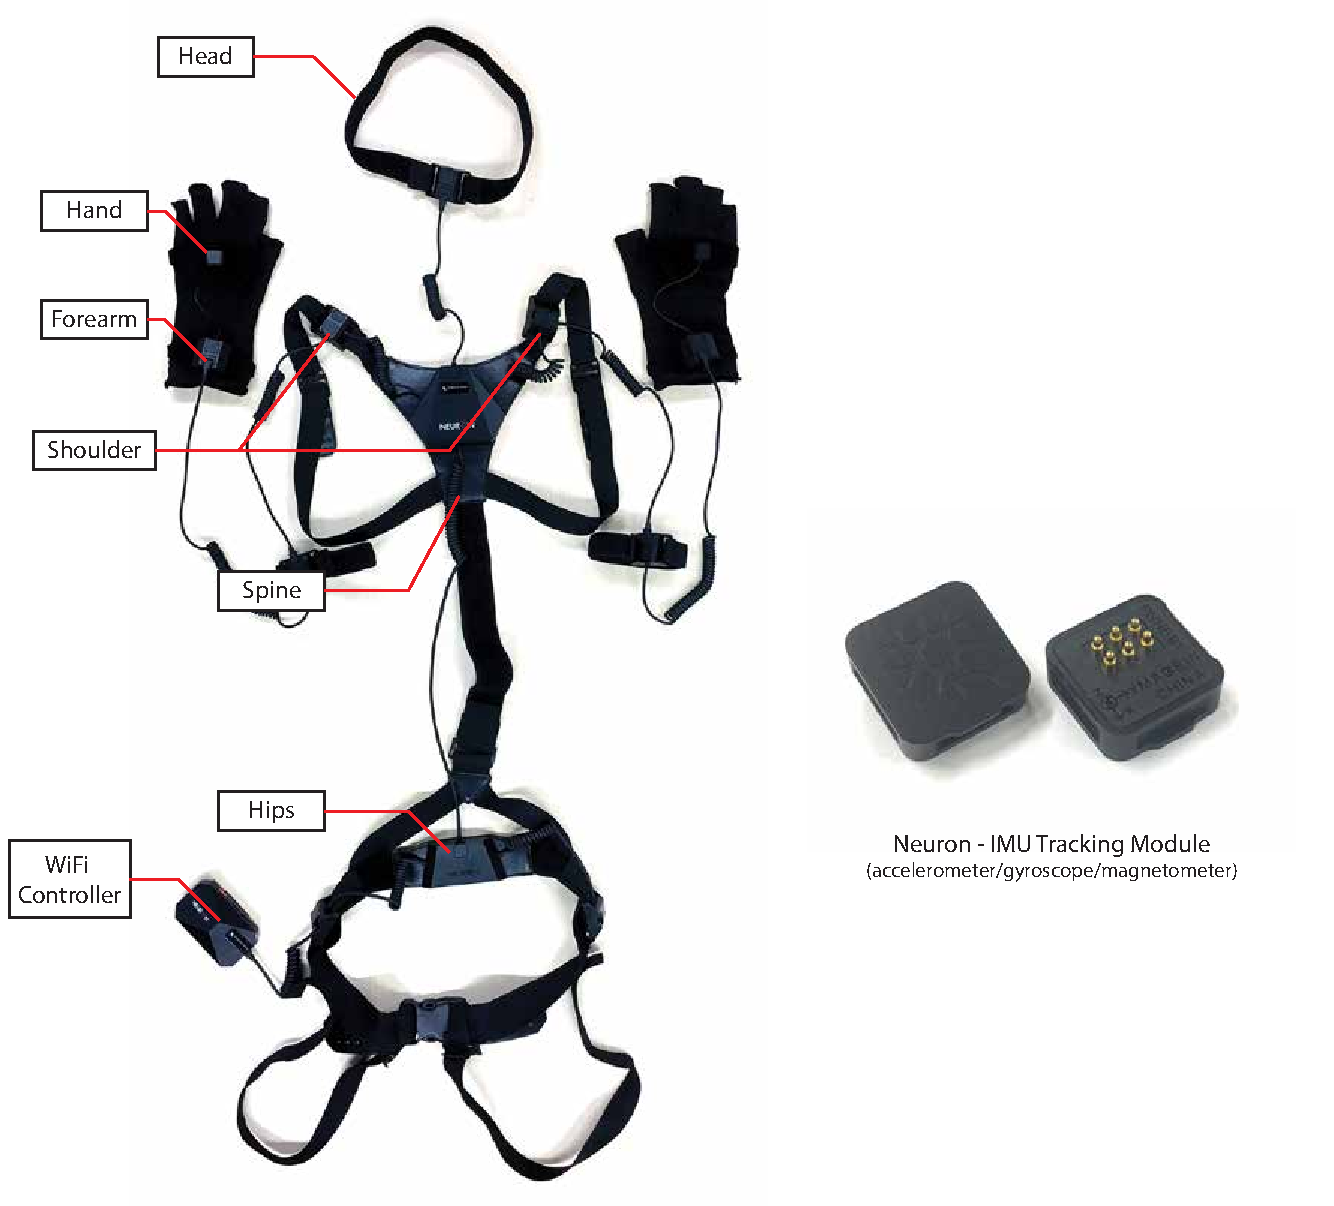
\includegraphics[width=0.8\textwidth]{figures/system/NeuronPerceptron.pdf}
\caption{Full body tracking system (Neuron Perception).}
  \label{fig:system-neuron-overview}
\end{figure}

\begin{figure}[t!]
\centering
\captionsetup{justification=centering} 
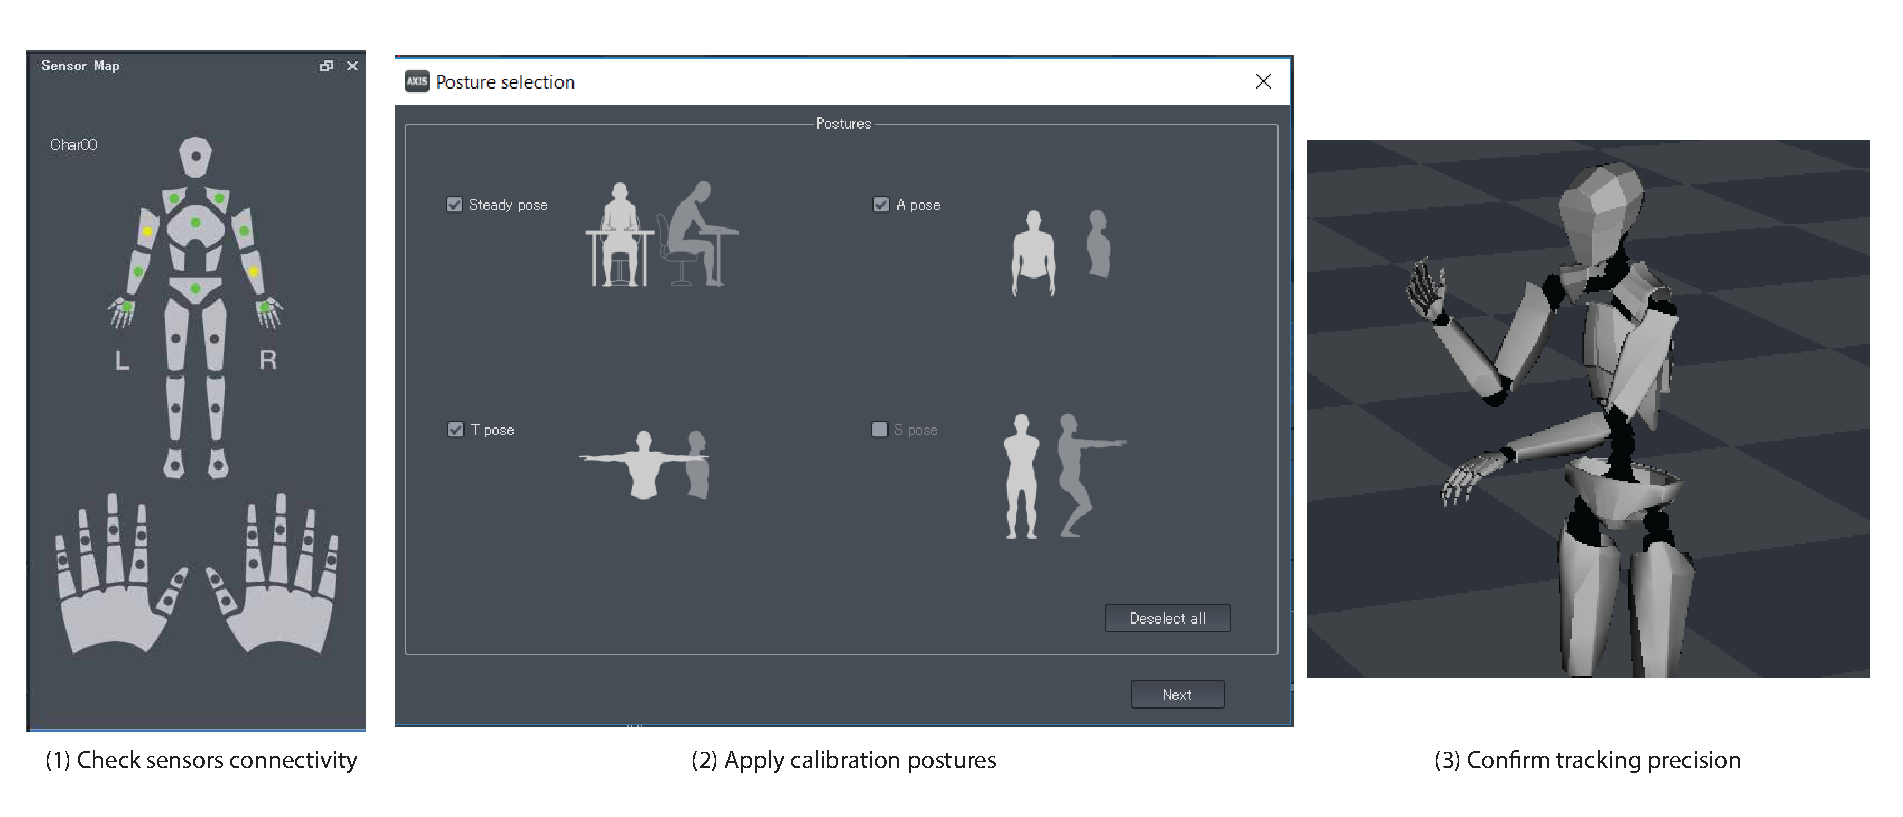
\includegraphics[width=1\textwidth]{figures/system/NeuronCalibration.pdf}
\caption{Calibration process for Neuron Perception system.}
  \label{fig:system-neuron-calibration}
\end{figure}



A combination of multiple systems is also possible in order to acquire the highest robustness with minimum complexity while maintaining the number of joints tracked. For example, to use Oculus HMD to track the head motion while providing the visual and auditory feedback to the user combined with 5DT data glove to track fingers posture, and overall body tracking using Neuron Perception system. 

As part of body state quantification modeling, eye gaze modality provides important information about the area of interest the user is looking at. This modality can be used as supportive input for multi-modal interaction as will be described later in operation and model alteration meta-models. An pupil tracking system was used by embedding dual cameras into the head mounted display. The system uses infrared cameras located behind the lenses of the HMD, and a half mirror placed at $45\deg$. Five infrared LED emitters are embedded into the lens which illuminate the eye pupil. The camera captures the reflected light of the eye via the half mirror. An illustration of the system is shown in \Figure{fig:system-pupillabs-overview}. A custom plugin for Unity3D was developed and integrated which communicates with the camera software. The plugin carries on the calibration procedure which is required per-user before start using the trackers. A 9-points eye fixation calibration is integrated, which maps the captured pupil locations with pre-defined points in 2D space. 120 samples per point (which is about 2 seconds per eye for 60 FPS tracking, in total 18 seconds for all points ) provided good balance between calibration time and accuracy of tracking.

The last modality for capturing user's state is the speech modality. The audio from user side is captured from an attached audio input interface. Although in most cases only a single audio input interface is needed to capture the state of user's speech, however the model supports the use of multiple audio interfaces. For example, in multiple audio input case, its possible to triangulate the position of the audio source using the volume. These types of use cases are application dependant.


\begin{figure}[t!]
\centering
\captionsetup{justification=centering} 
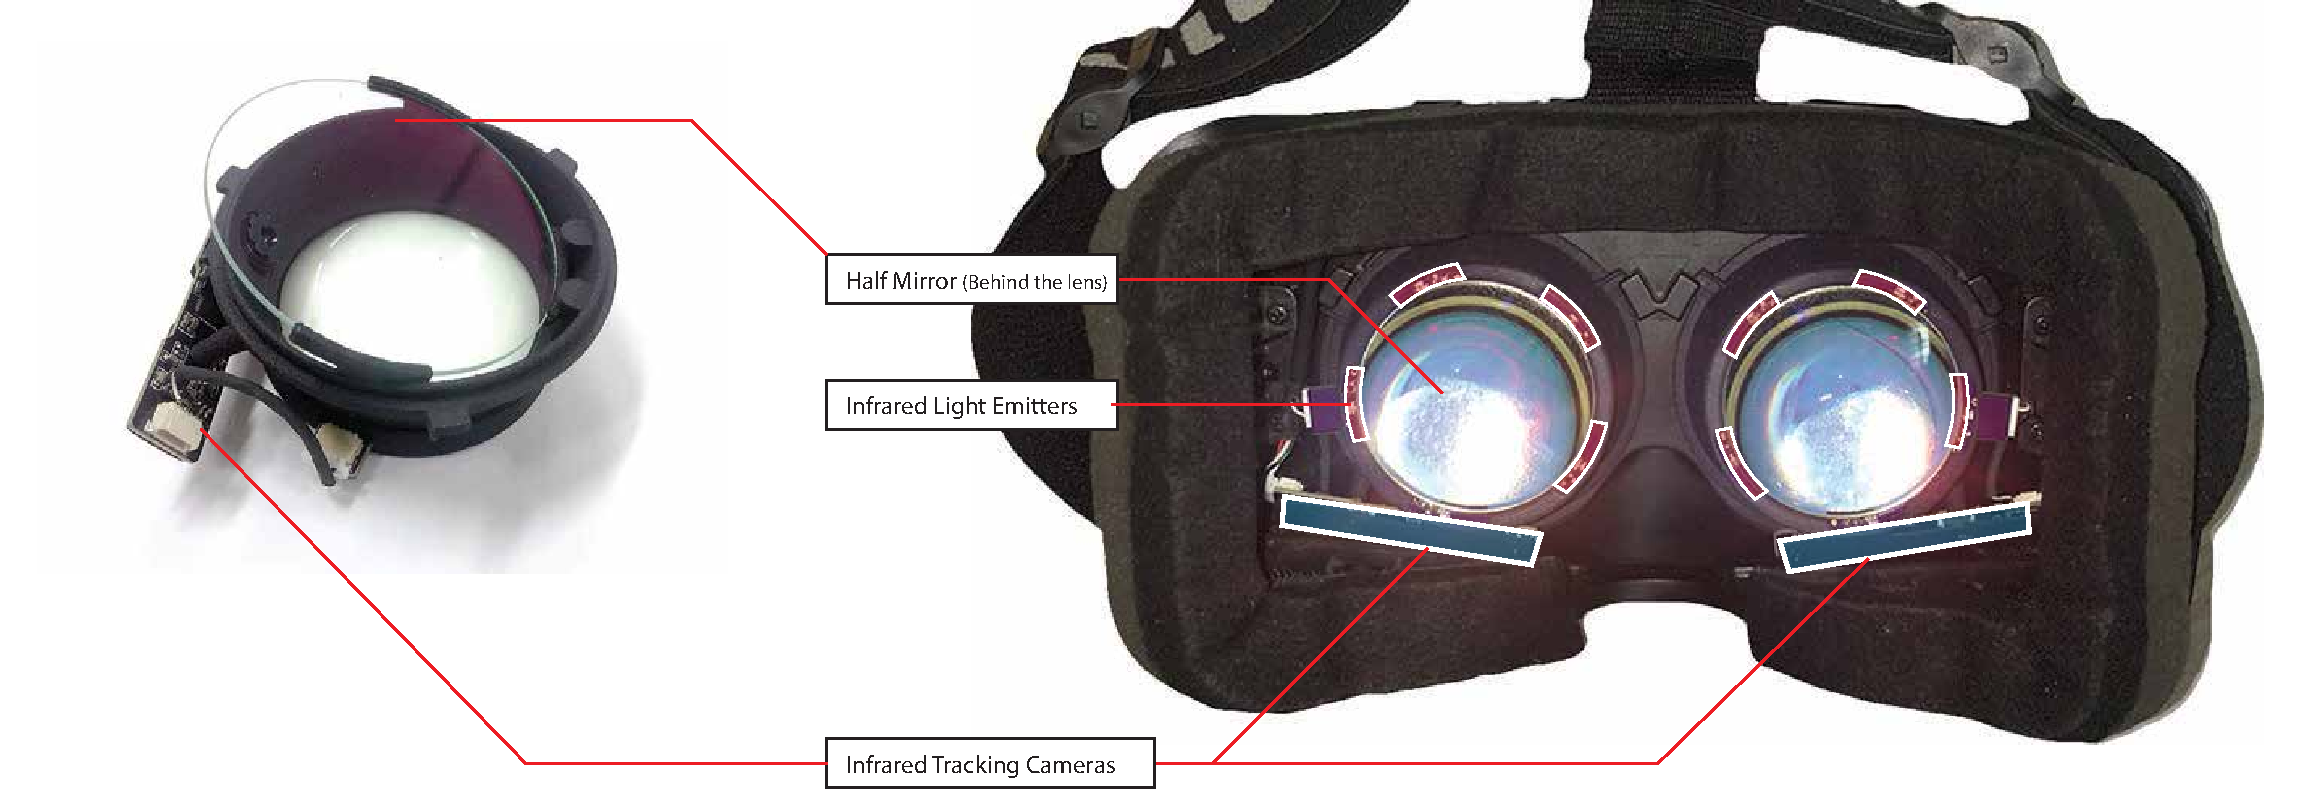
\includegraphics[width=1\textwidth]{figures/system/PupilTracker.pdf}
\caption{Eye tracking module used (PupilLabs + Oculus DK2).}
  \label{fig:system-pupillabs-overview}
\end{figure}




To use in the meta-modeling editor, the tracking systems were encapsulated and integrated as meta-blocks shown in \Figure{fig:system-trackers-blocks}:
\begin{itemize}
\item OptiTrack Block: Communicates with an optiTrack server that runs the tracking system. The node requires to specify the target server IP address. For each block, the name of the target tracked object should be specified in its block parameters. When the meta-model runs, the object data is output as [Joint] data channel.

\item HMD Block: Handles the tracking of the connected HMD. The block provides two outputs: [Joint] for the spatial position and orientation of the HMD, and [Mounted] as a boolean channel indicating whether the HMD is being used or not (compatible with Oculus CV1/HTC Vive HMDs).

\item Neuron Block: Similar to OptiTrack Block, it also requires to specify the server IP address running Neuron Perception service. This node requires to specify the ActorID when more than one tracking suit is being connected. The block outputs [Body] data structure containing the entire tracked body joints data.

\item Leapmotion Block: Provides accessibility functions to leapmotion tracking. Requires to specify the target hand to track (Left or Right), and it outputs [Hand] data. [Fist] provides whether the hand is closed or not as floating point value.

\item 5DT Data Glove Block: Similar to Leapmotion, requires to specify the target hand to track, and it outputs fingers information on the [Hand] output channel.


\begin{figure}[t!]
\centering
\captionsetup{justification=centering} 
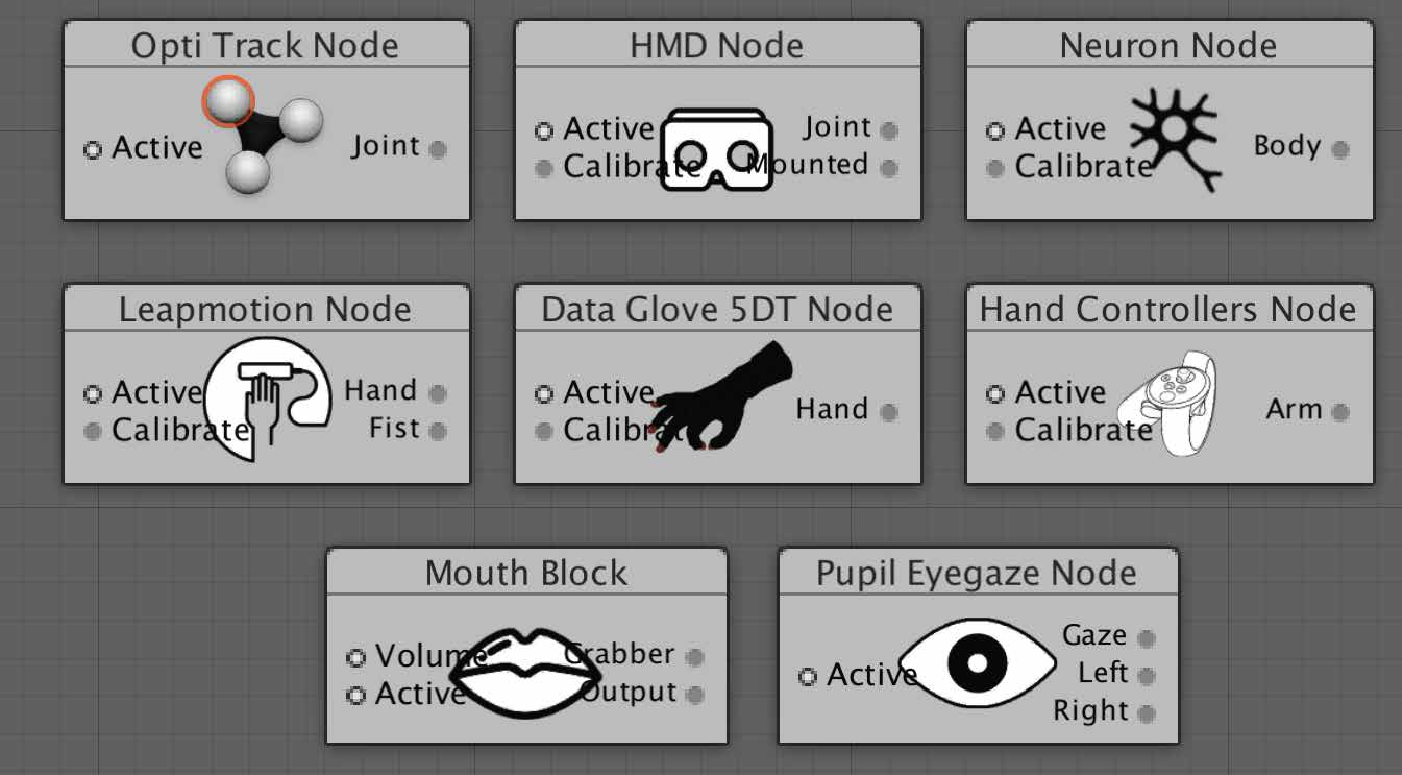
\includegraphics[width=1\textwidth]{figures/system/Blocks/Trackers.pdf}
\caption{Body state tracking blocks.}
  \label{fig:system-trackers-blocks}
\end{figure}

\item Hand Controllers Block: Uses Oculus Touch to track hands position and fingers bending. Outputs [Arm] structure containing the estimated position of the hand relatively to the HMD position.

\item Mouth Block: Connects to an audio input interface, and provides the sampled audio on [Output] channel. It is possible to indicate the sampling rate in its settings, default set to 16,000Hz.

\item Pupil Eyegaze Block: Uses the functionality of Pupillabs eye tracking hardware to measure the pupil gaze position. Outputs both [Left] and [Right] values for both eyes, and the estimated looking position on [Gaze] channel. Data used is a 2D value vector [Vector2].

\end{itemize}




\subsubsection{Feedback Blocks}
%ears 
%mouth


Feedback blocks mainly communicates the meta-model perceptual states back into the user. Within the current scope of this thesis, three different types of feedback modalities are explored and integrated into the EDD framework and meta-modeling editor:


\begin{figure}[b]
\centering
\captionsetup{justification=centering} 
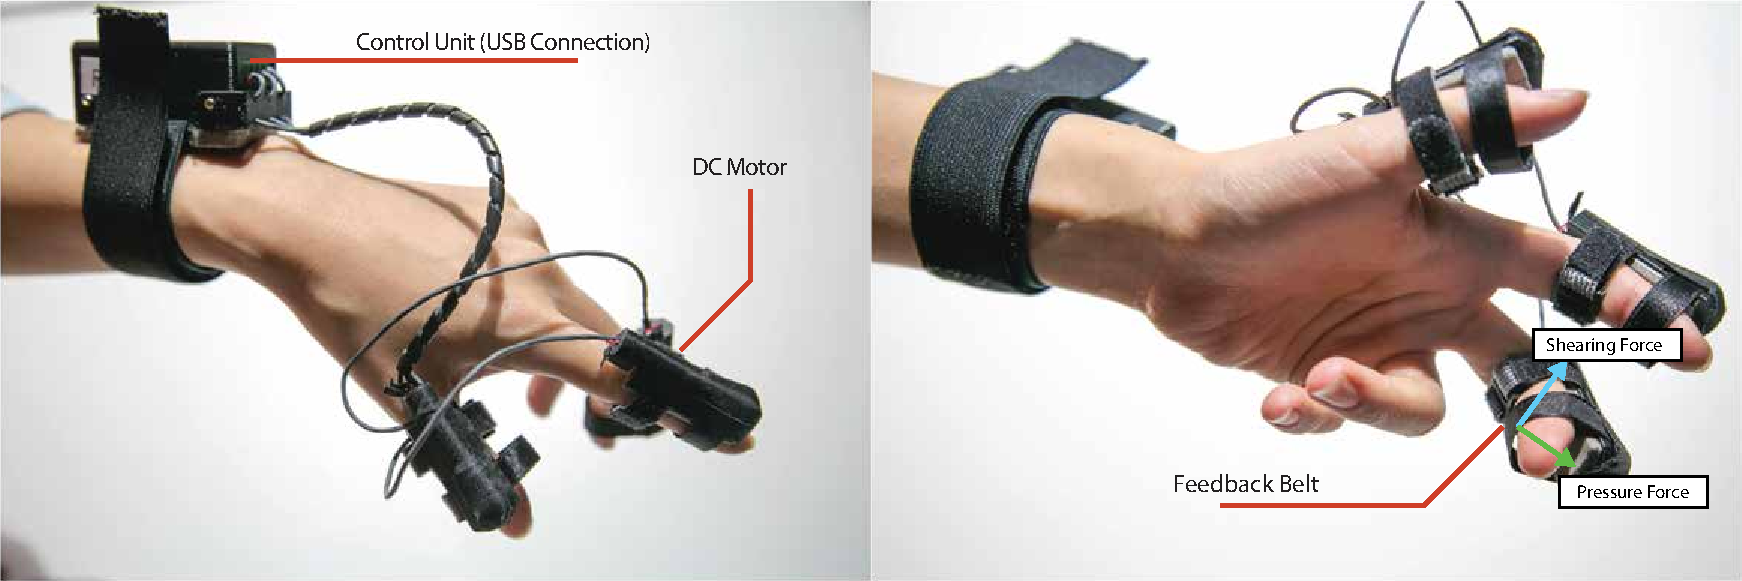
\includegraphics[width=1\textwidth]{figures/system/GGDisplay.pdf}
\caption{Fingers force feedback display.}
  \label{fig:system-GGDisplay}
\end{figure}

$\bullet$ Visual Feedback: transforms stereo images input into a displayable format to be presented into the user's vision. The visuals are directed into [Vision] data type which contains dual textures of type Texture2D. These images are either captured from representation blocks, or are generated from transfer blocks. Depending on the display device used (HMD, Monitor, ...etc), parameters related to the field of view and aspect ratio of the device should be specified. In the meta-blocks, these functionalists are encapsulated and are automatically calculated, however it is still possible for the designer to alter these settings.

$\bullet$  Auditory Feedback: plays back audio samples stream into an output audio interface at the user's side, and represented as [Ears] module. Samples are encapsulated into an [Audio] data type that can handle multiple audio channels, and different sampling rates. For audio playback, the sampling rate by default is set to 48,000Hz, but can be changed by the designer.

$\bullet$ Haptic Feedback: communicates with a haptic interface connected to the user's side, and can provide both force and tactile feedback information into the device. Both data are represented using [Haptic] data structure. Force feedback is a three-directional vector3 which provides the 2D (X, Z) tangential force along the surface of the display, and the perpendicular (Y) pressure force on the display surface. Currently, Gravity Grabber \cite{minamizawa2007gravity} type of displays are supported for force feedback. A custom display has been developed which can provide horizontal (X) shearing forces, and the perpendicular (Y) pressure forces for three fingers of each hand \Figure{fig:system-GGDisplay}. For tactile feedback, the data is stored as an array of floating points within the range of [-1,1] representing the signal captured by a vibrotactile sensor, or generated in software using a transfer block. The sampling rate for this signal is less than 2000Hz samples (representing a maximum frequency of 1000Hz which is the limit of Pacinian corpuscle receptors in the skin). To display the tactile data, a vibrotactile actuator can be used by directly connecting it to an output audio interface and specify the interface ID in the settings of the haptic block.

\begin{figure}[htbp]
\centering
  \captionsetup{justification=centering}
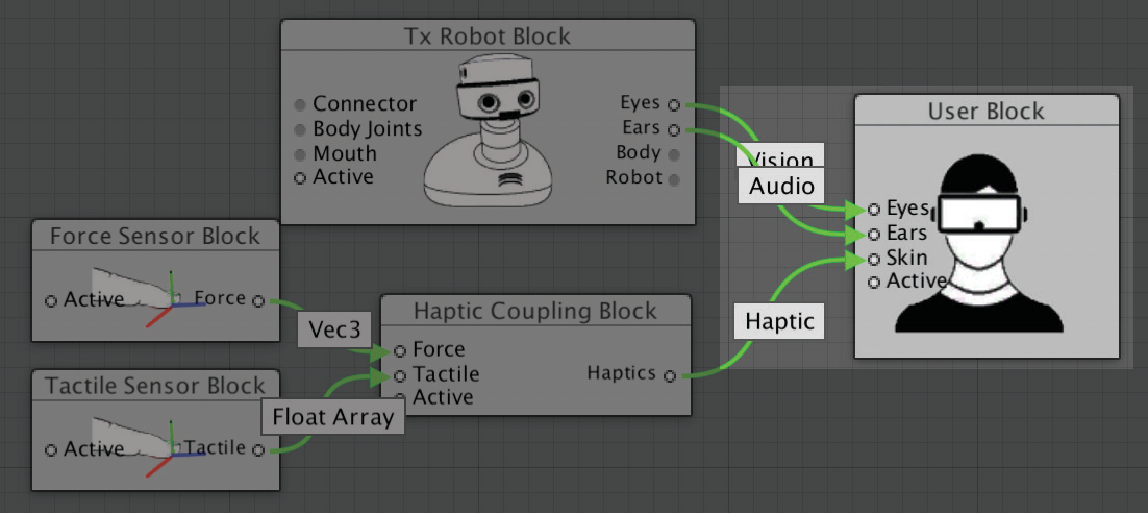
\includegraphics[width=0.8\textwidth]{figures/system/Blocks/UserBlock.pdf}
\caption{User feedback block meta-model example.}
  \label{fig:system-userblock}
\end{figure}

Since all these modalities are related to the user feedback, a single [User] block \Figure{fig:system-userblock} that provides the functionality to receive the various perceptual input has been designed and integrated into the meta-modeling editor. The block receives three inputs representing the Eyes, Ears, and Skin modalities that corresponds to the visual, auditory, and haptic feedback respectively.



\subsection{Representation Blocks}

This set of meta-blocks communicates with the used body representation. It facilitates the process of transferring the information flow between the meta-model and the representation type used. Two main types of representations are used in this thesis: physical and virtual type. The physical type communicates with a robotic form located at the user side as a peripheral device, or remotely connected over the network, and controls its physical state such as servo link driving or captures sensory information from it, such as tactile sensors. And the virtual type mainly communicates with Unity3D editor into a virtual character (humanoid or non-humanoid) to control its body postural. Generally speaking, representation model blocks are considered as mirroring the functionality of perceptual model, that is the for each input of representation blocks a corresponding output from perceptual blocks and vice versa.

The first block type for the body model is the postural blocks. The control mechanism for the postural of the representation is driven by the [Body] data type that defines the new body schema from the user. Different approaches for control is dependant on the \textit{Representation Engineer} choice. For example, the driving can be done using Forward Kinematics (FK) model (direct drive) in which the joints angle is directly applied from the input body joints data. For example, 3 DoF telexistence robot uses forward kinematics to drive the head motion of the robot from the head joint of the body. A 6 DoF robot (with parallax motion type) would use a different approach to calculate robot's joints angle from head position, using Inverse Kinematics (IK) model to drive the parallax joints from head position and rotation. The postural blocks should provide compatible data channel to the representation used, for example a network-based communication is used, a combination of UDP and TCP protocols can be used to bridge the data flow from Unity3D to the robot side, and for peripherals connected directly to the user side pc, a serial communication protocol can be used to deliver the control signals to the used peripheral. The EDD framework provides an abstraction to the communication protocol used, so the same block can be reused for different representations. The  \textit{Representation Engineer} can either develop new protocols to communicate with the hardware used, or to build on to of the exciting protocols used in the framework. The physical toolkit in \Section{impl:toolkit} provides building blocks for developing the representation hardware while maintaining the support to EDD framework representation blocks. The toolkit discussed also includes important details about media streaming optimization for various types of sensory modalities, mainly for the real-time visual feedback. 

\begin{figure}[htpb]
\centering
  \captionsetup{justification=centering}
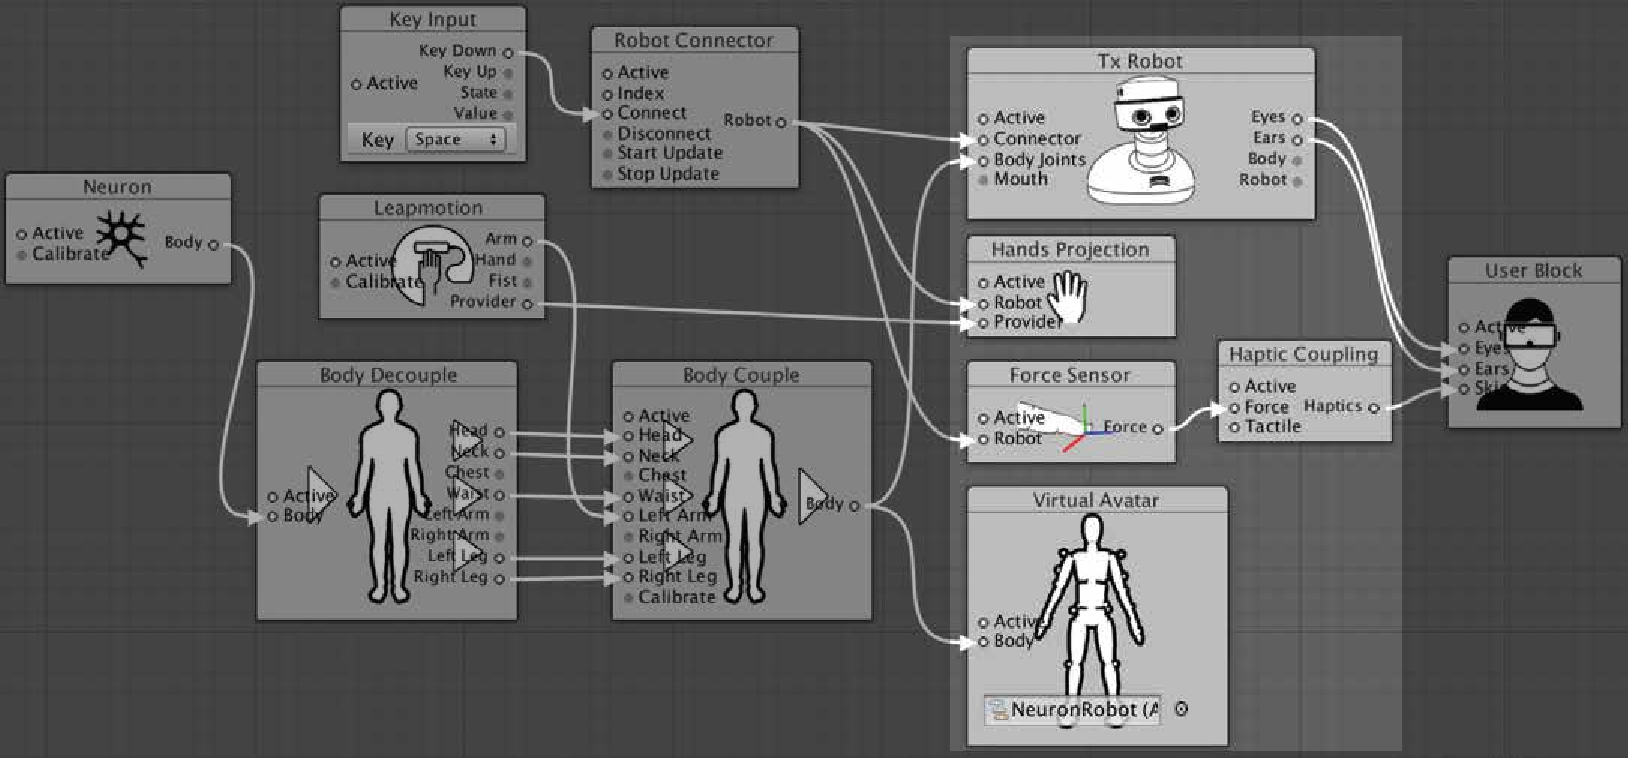
\includegraphics[width=1\textwidth]{figures/system/Blocks/Representation.pdf}
\caption{Using multiple blocks types for representation.}
  \label{fig:system-representatio-blocks}
\end{figure}


The other block type for the representation blocks is the sensory blocks. These blocks are responsible to deliver various modalities information back to the meta-modeling editor. \Figure{fig:system-representatio-blocks} shows an example of using both postural and sensory representation blocks used in parallel for two different types of bodies. [TxRobot] block encapsulates the postural modality function, and provides the sensory feedback on its outputs. The [Force Sensor] is used as a separate module since the number of sensors can vary based on the application. [Hands Projection] block provide the functionality for representation alteration meta-modeling in which it streams the virtual representation of the hands into the robot side. Finally, [Virtual Avatar] block communicates with Unity3D character model to control its postural state based on the shared [Body] input. In this example, both representations are driven by the same body input.



\subsection{Transfer Blocks}

The final category of meta-blocks is the Transfer type. This category contains a wide variety of functions and modifiers which can be general purpose type (e.g. mathematics, image processing, body mapping alteration, ...etc) to a very application specific blocks (e.g. layered perception, motion transformation, ...etc). 

\begin{figure}[htpb]
\centering
  \captionsetup{justification=centering}
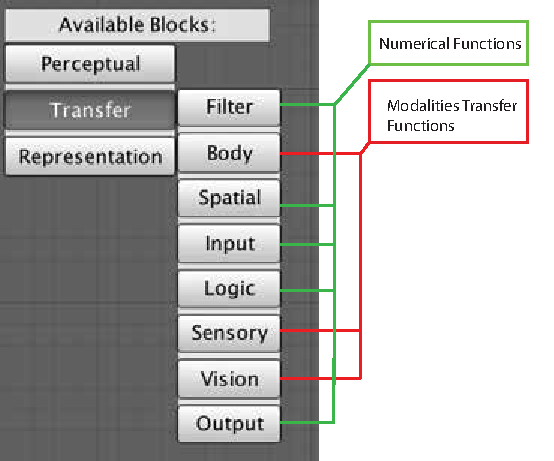
\includegraphics[width=0.8\textwidth]{figures/system/Blocks/TransferBlocks.pdf}
\caption{List of transfer blocks sub categories.}
  \label{fig:system-transfer-blocks}
\end{figure}

The transfer blocks are used as a middle function to modulate the data flow between the representation and user blocks. Also it can be used to apply logic operations on perception, for example activate or disable certain modalities channels flow based on behaviours or body state. A list of transfer blocks categories is shown in \Figure{fig:system-transfer-blocks}.


\begin{figure}[t!]
\centering
  \captionsetup{justification=centering}
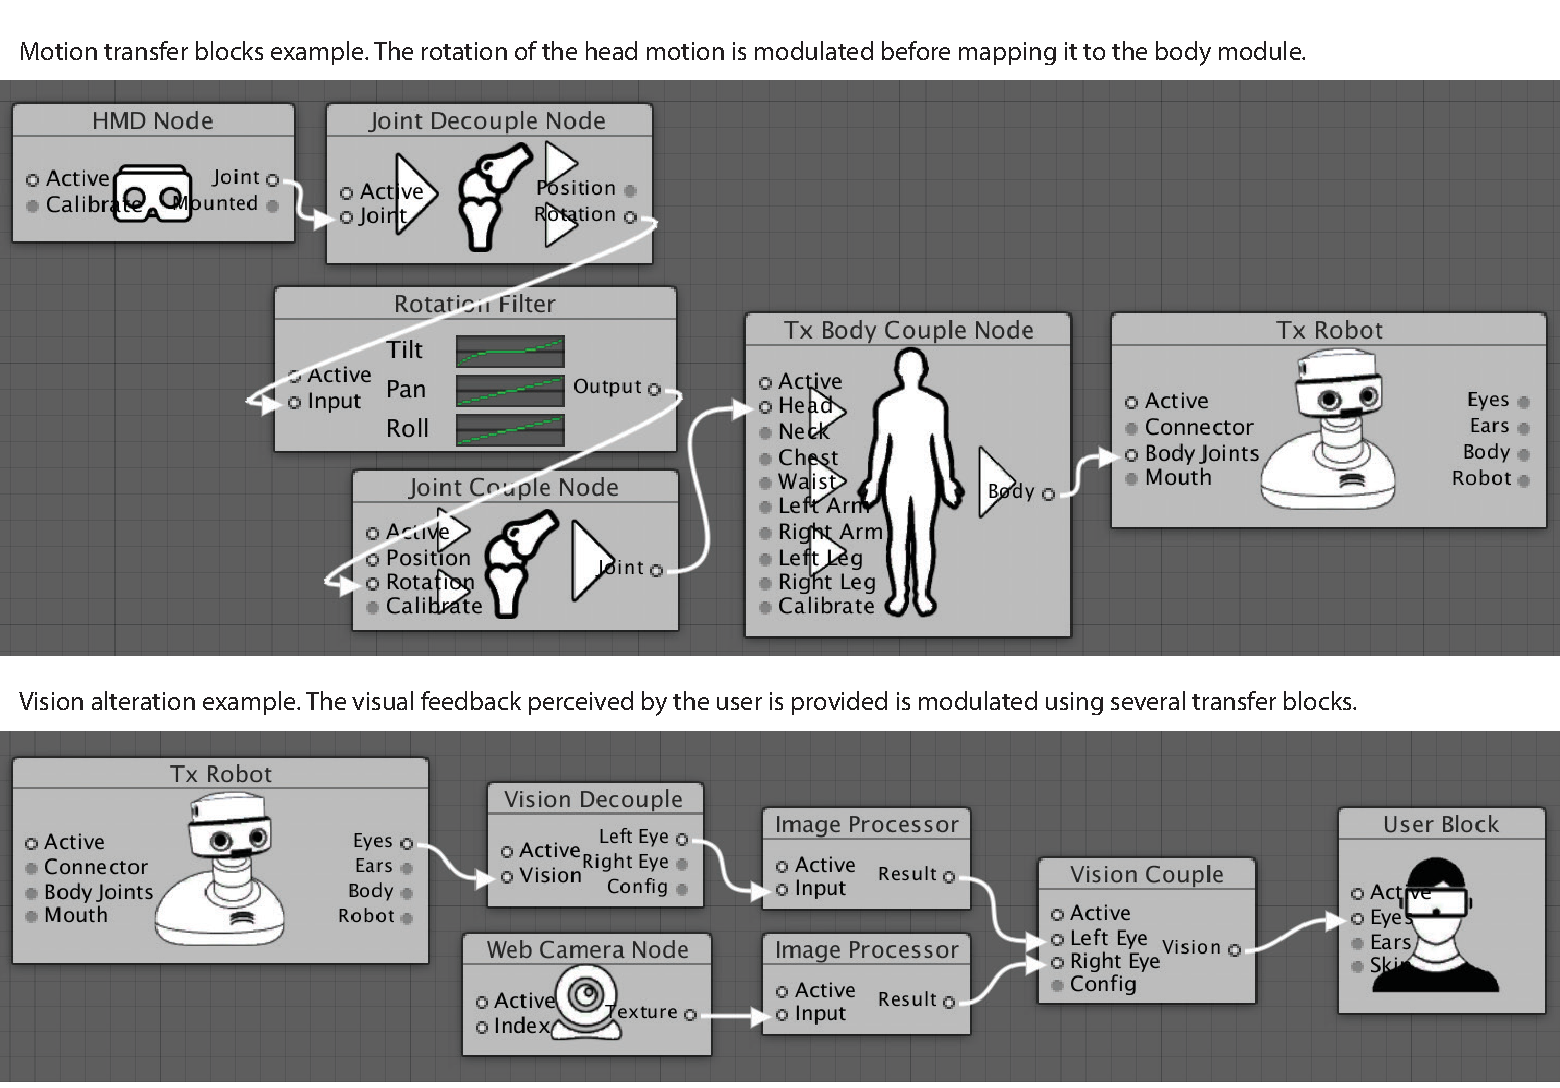
\includegraphics[width=1\textwidth]{figures/system/Blocks/TransferExample.pdf}
\caption{Examples of using transfer blocks to modulate body and visual modalities.}
  \label{fig:system-transfer-example}
\end{figure}

Examples of using transfer blocks to modulate body mapping and perception feedback are shown in \Figure{fig:system-transfer-example}. The first example highlights the use of spatial alteration filter block [Rotation Filter] to modulate head joint rotation into a nonlinear mapping. Three different mapping curves can be defined for each rotational axis (Tilt, Pan, Roll), which acts as a function for each angle. The second example shows a higher level of perception editing. In this example, the vision input modality for the user is altered using two different sources. The robot block's vision is decoupled into separate eyes using [Vision Decouple] transfer block, and then is processed using [Image Processor] transfer block. The image processor block uses a program written in shader language (HLSL) which runs inside the block process to produce a new image on its Result output channel. Robot's vision is mapped into the left eye of the user, while the right eye is mapped to a different source using [Web Camera] representation block. 



\section{Physical Toolkit Development}
\label{impl:toolkit}

As a part of realizing the idea of Embodied-Driven Design on a larger scale, a general purpose physical toolkit was developed through several iterations and prototypes along the development of embodiment framework and the meta-modeling editor. The toolkit design considerations were discussed previously in the design chapter in \Section{concept:toolkit}. The implementation process and details of this toolkit is discussed here.

An overview of the different prototypes that has been developed is illustrated in \Figure{fig:system-txkit-iterations}, and the description of each iteration considerations and requirement is shown in \Table{fig:system-txkit-iterations}. Iterations A-B were highly application specific designs and mainly used for representation alteration purpose. Iteration C was a base step for developing higher performance toolkit using better optics and vision system than the previous generations, and has been used as a part of model alteration meta-modeling. And iteration D is the current design which provides a balance between performance and usability. 

Along the hardware development of the robots, a corresponding software architecture was developed to facilitate the usability of the toolkit and to make it compatible with the Embodiment framework. Both the hardware and the software are highly modular and reusable. 

\begin{figure}[htbp]
\centering
\captionsetup{justification=centering} 
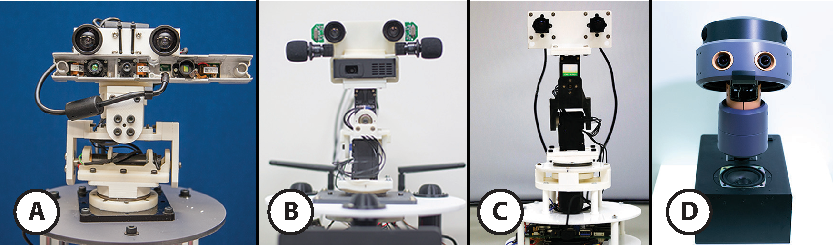
\includegraphics[width=1\textwidth]{figures/system/TxKitIterations.pdf}
\caption{Physical toolkit design iterations. }
  \label{fig:system-txkit-iterations}
\end{figure}


\begin{table}[t!]
\footnotesize
\centerline{
\begin{tabular}{|l|l|l|l|l|}
\hline
\rowcolor[HTML]{C0C0C0} 
\textbf{Iteration}                                                                             & \textbf{A}                                  & \textbf{B}                                       & C                                                           & D$^{*}$                                                           \\ \hline
\cellcolor[HTML]{EFEFEF}\textbf{\begin{tabular}[c]{@{}l@{}}Development \\ Year\end{tabular}}   & 2014                                        & 2015                                             & 2016                                                        & 2017                                                       \\ \hline
\cellcolor[HTML]{EFEFEF}\textbf{Application}                                                   & \multicolumn{2}{c|}{\begin{tabular}[c]{@{}c@{}}Enforced \&\\ Mutual Telexistence\end{tabular}} & \begin{tabular}[c]{@{}l@{}}Layered \\ Presence\end{tabular} & \begin{tabular}[c]{@{}l@{}}General \\ Purpose\end{tabular} \\ \hline
\cellcolor[HTML]{EFEFEF}\textbf{Requirement}                                                   & Depth Sensor                                & Projection Module                                & High performance                                            & Usability                                                  \\ \hline
\cellcolor[HTML]{EFEFEF}\textbf{\begin{tabular}[c]{@{}l@{}}Meta-Model\\ Category\end{tabular}} & \multicolumn{2}{c|}{\begin{tabular}[c]{@{}c@{}}Representation \\ alteration\end{tabular}}     & \begin{tabular}[c]{@{}l@{}}Model\\ alteration\end{tabular} & -                                                          \\ \hline
\end{tabular}
}
%\footnotesize 
\begin{tablenotes}
%\captionsetup{justification=justified,format=plain, font=small} 
\item $^{*}$Developed in a collaboration with Karakuri Products, Inc.
\end{tablenotes}
\centering
\caption{Toolkit design iterations and considerations.}
\label{table:system-toolkit-iter}

\end{table}


%\subsection{Postural Design: Head Motion}
    

\subsection{Hardware Design}

\begin{figure}[htpb]
\centering
  \captionsetup{justification=centering}
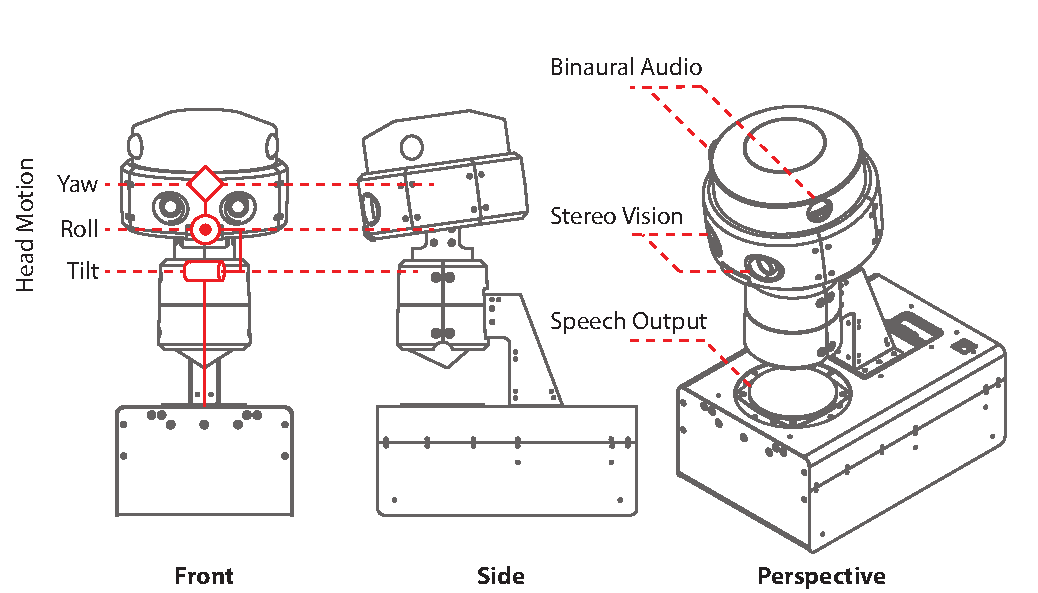
\includegraphics[width=1\textwidth]{figures/system/TxKitDesign.pdf}
\caption{Physical toolkit hardware schematic design.}
  \label{fig:system-txkit-schema}
\end{figure}

The schematic design of the latest toolkit is shown in \Figure{fig:system-txkit-schema}. This design provides the essential modalities for creating general purpose presence experience:
\begin{itemize}
  \setlength\itemsep{0em}
  \item \textbf{Vision:} Stereo camera with fixed interpupillary distance of 65mm (using camera model Ovrvision Pro, or See3CAM CU130 by e-consystems). Each camera has different specifications, but both are suitable for human oriented vision. \Table{table:system-toolkit-cams} provides a list of the important details regarding the selection of the cameras.
  \item \textbf{Auditory:} Binaural microphone set (Audio Technica AT9911). 
  \item \textbf{Communication:} Audio output speaker with an omni-directional design. A custom audio amplifier was added for controlling audio levels. 
  \item \textbf{Body structure:} Motion control using 3 Axis head (Pitch, Yaw, Roll). Servo type motors were used to control rotation position of the robot head motion (Kondo Robots model KRS-4031HV ICS/KRS-4032HV ICS). The mechanical limits for each of the three axes is shown in \Table{table:system-toolkit-motion}.
\end{itemize}





\begin{table}[htpb]
\footnotesize
\begin{tabular}{|l|l|l|}
\hline
                                                   & \cellcolor[HTML]{EFEFEF}\textbf{\begin{tabular}[c]{@{}l@{}}See3Cam\_CU13\\ +H0320KP (S Mount Lens)\end{tabular}} & \cellcolor[HTML]{EFEFEF}\textbf{Ovrvision Pro}                                                          \\ \hline
\cellcolor[HTML]{EFEFEF}\textbf{Count}             & 2                                                                                                                & 1 (stereo camera on board)                                                                              \\ \hline
\cellcolor[HTML]{EFEFEF}\textbf{Image Stitching}   & Software stitch (unsynced)                                                                                       & Hardware stitch (synced)                                                                                \\ \hline
\cellcolor[HTML]{EFEFEF}\textbf{Supported Formats} & \begin{tabular}[c]{@{}l@{}}640x480@60\\ 1280x720@60\\ 1920x1080@30\end{tabular}                                  & \begin{tabular}[c]{@{}l@{}}640x480@90\\ 960x950@60\\ 1280x800@60\\ 1920x1080@30\end{tabular}            \\ \hline
\cellcolor[HTML]{EFEFEF}\textbf{USB Connections}   & 2 x USB3.0                                                                                                       & 1 x USB 3.0                                                                                             \\ \hline
\cellcolor[HTML]{EFEFEF}\textbf{Field of View}     & 89x67                                                                                                            & 115x105                                                                                                 \\ \hline
\cellcolor[HTML]{EFEFEF}\textbf{Quality}           & \begin{tabular}[c]{@{}l@{}}High quality \\ (Raw image from sensors)\end{tabular}                                 & \begin{tabular}[c]{@{}l@{}}Low$\sim$Medium Quality \\ (compression and optics)\end{tabular} \\ \hline
\end{tabular}
\centering
\caption{A comparison between the used cameras in the toolkit.}
\label{table:system-toolkit-cams}
\end{table}


\begin{table}[htpb]
\begin{tabular}{|
>{\columncolor[HTML]{C0C0C0}}l |l|l|}
\hline
Axis & \cellcolor[HTML]{EFEFEF}Min{[}-180,180{]} & \cellcolor[HTML]{EFEFEF}Max{[}-180,180{]} \\ \hline
Tilt & $-20\deg$                     & $20\deg$                      \\\hline
Yaw  & $-90\deg$                     & $90\deg$                      \\\hline
Roll & $-20\deg$                     & $20\deg$                     \\\hline
\end{tabular}
\centering
\caption{Head rotational mechanical limits.}
\label{table:system-toolkit-motion}
\end{table}

\subsection{Software Architecture}
The LCM design pattern is reflected in the design architecture of the software for the framework. \Figure{fig:system-txkit-software} shows the major components used in the framework design and the implementation of the representation blocks. The software is distributed along two sides: robot side, and user side. In the current implementation, the robot side provides the following five services:

\begin{itemize}
  \setlength\itemsep{0em}
  \item \textbf{TxEyes:} responsible for camera access and streaming, handles image capture, encoding, and sending to the user side. Supports the following camera types: 
  \begin{itemize}
  \setlength\itemsep{0em}
  \item Directshow UVC camera drivers, such as webcams.
  \item Ovrvision Pro camera.
  \item Ricoh Theta omni directional camera.
  \end{itemize}
  Video latency in this system is measured to $180\pm20$ms when streaming dual images of size 640x480 at 60 frames per second on a LAN.
  \item \textbf{TxBody:} communicates with the hardware and servo motors. The following body architectures are supported:
  \begin{itemize}
  \setlength\itemsep{0em}
  \item Three axis head control (Pitch, Yaw, Roll).
  \item Six axis body control, such as Torso type systems, controlled by head position \& rotation six values tuple (X,Y,Z,Pitch, Yaw, Roll).
  \item Drone type systems, driven by speed vector for position \& rotation (Speed X,Y,Z/Rotational speed Theta, Gamma, Alpha).
  \end{itemize}
  \item \textbf{TxEars:} provides access to audio hardware, capture, encode and streaming audio data over network to user side. Number of audio channels can be set, by default 2 audio channels (Left, Right) are configured.
  \item \textbf{TxMouth:} handles audio stream input from user side, and responsible for audio playback on the robot side.
  \item \textbf{TxHands:} responsible of displaying operator's body images from an egocentric point of view. Compatible with projector modules.
\end{itemize}



\begin{figure}[t!]
\centering
  \captionsetup{justification=centering}
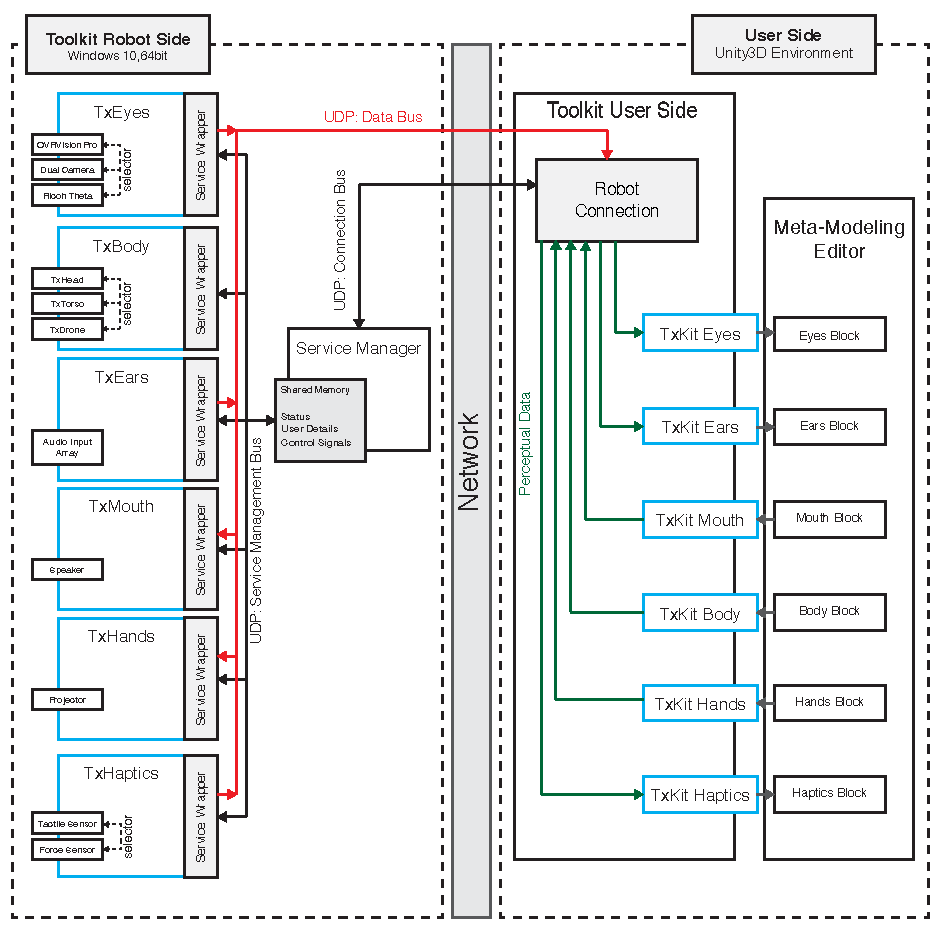
\includegraphics[width=1\textwidth]{figures/system/TxKitSystem.pdf}
\caption{Toolkit software architecture.}
  \label{fig:system-txkit-software}
\end{figure}

Each of these modules is encapsulated as a service, and runs on a separate process in the system, and communicates with a service manager that hosts them over UDP protocol. \Figure{fig:system-txkit-services} shows four different types of services running on the robot side. Each service provides information of their state, as well as the overall resources being consumed by the service (CPU, virtual \& physical memory consumption). A shared memory is used between the processes to provide direct and quick access to the status of the system, user's address, and other control messages. This design provides maximum stability over the system runtime, and reduces the chances of process crashes. Also, as mentioned before, these modules (or services) can run individually depending on the design requirements. For media streaming, encoding, and decoding, GStreamer library was used \footnote{https://gstreamer.freedesktop.org/}. GStreamer is an open source multimedia library which encapsulates the core functions for general video and audio encoders/decoders. In the robot side, H.264 codec was used for video encoding, and Opus codec for audio encoding. Both encoders proved to be the most efficient encoders in term of low latency performance.


\begin{figure}[htpb]
\centering
  \captionsetup{justification=centering}
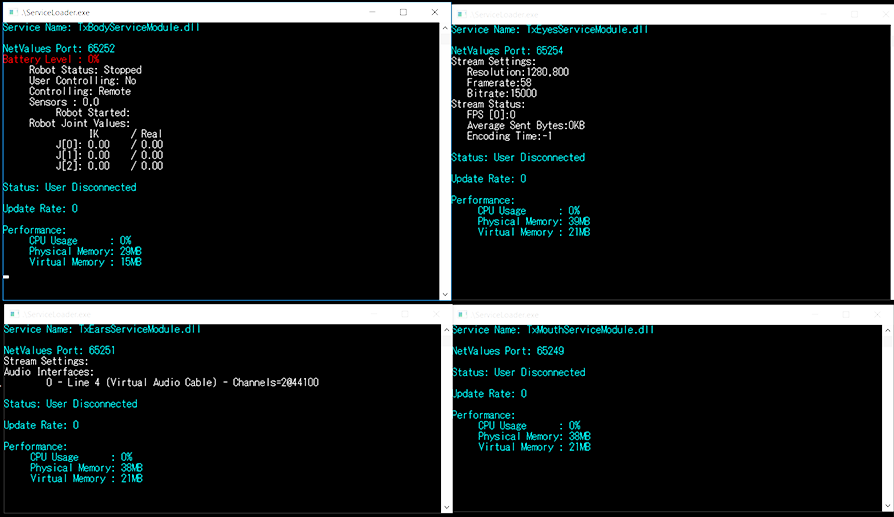
\includegraphics[width=1\textwidth]{figures/system/Services.png}
\caption{Service modules operating on toolkit side.}
  \label{fig:system-txkit-services}
\end{figure}

On the user side, modules are defined to handle the actual communication with the representation. Each of these modules corresponds to a representational block (Eyes, Ears, Mouth, ...etc). The software on the user side is implemented for Unity3D Editor integration under Windows operating system, as this game engine is considered as one of the most user friendly environments for virtual reality related application design.





\subsection{Video Streaming Evaluation}
For achieving close real-time perception streaming over the network, and to minimize the overall latency from the robot side to the user side, an optimized media tool-set were developed and used in toolkit. In the conducted tests, visual latency and image quality were the major considerations in the system design, which they affected the overall experience in robot operation. 

In order to evaluate the streaming performance, a custom measurement software has been developed which calculates the capture-to-display latency of the cameras. The latency measurement system is shown in \Figure{fig:system-txkit-latencymeasure}. To use this system, both the robot side containing the camera to be tested, and the user side should be located physically together. The system uses a display located at the user side that outputs a series of black/white frames which the camera of the streaming side captures. When a frame is displayed, the system records the current time stamp in milliseconds and waits before generating the next frame. The camera side captures, encodes the images into a compressed format such as H264 encoding, and streams the encoded images as a RTP data into the user side over the network medium using UDP protocol. The measurment side receives the RTP stream, decode it and compare the decoded image color value with the currently displayed frame. The system measures the cycle time (or latency time) by calculating the difference between the current timestamp and the displayed frame timestamp. 
 

\begin{figure}[htpb]
\centering
  \captionsetup{justification=centering}
\includegraphics[width=1\textwidth]{figures/system/LatencyMeasurment.pdf}
\caption{Camera capture-to-display latency measurement system.}
  \label{fig:system-txkit-latencymeasure}
\end{figure}

 
The camera module (Model no. See3CAM CU130 by e-consystems) used in the design of the third iteration has been evaluated for streaming performance over the network using the three different quality presets. \Table{table:camera-modes} shows the measured latency for each mode. 


\begin{table}[htpb]
\footnotesize
\begin{tabular}{|l|l|l|l|}
\hline
\rowcolor[HTML]{EFEFEF} 
{\color[HTML]{000000} \textbf{Quality}} & {\color[HTML]{000000} \textbf{\begin{tabular}[c]{@{}l@{}}Resolution\end{tabular}}} & {\color[HTML]{000000} \textbf{Framerate}} & {\color[HTML]{000000} \textbf{Latency (ms)}} 
\\ \hline
\textbf{Low Quality} & 640 x 480 & 60 &  $64\pm8$                                     
\\ \hline
\textbf{Medium Quality} & 1280 x 720 & 60 & $71\pm8$                                           
\\ \hline
\textbf{High Quality} & 1920 x 1080  & 30 &  $95\pm16$                                           
\\ \hline
\end{tabular}
\centering
\caption{Camera streaming quality modes and corresponding latency.}
\label{table:camera-modes}
\end{table}

\section{Vision Bandwidth Optimization}

In the previous section, the evaluation of the vision system showed an acceptable latency measurements (that is less than 100ms), however the effective spatial resolution of the encoded images is relatively low when high frame rate and low bandwidth were required. In this section, an optimization approach is proposed based on the human vision cues which would reduce the bandwidth and performance requirements significantly.

\subsection{Problem with current streaming systems}

Recent advances in virtual reality display systems began to offer end users immersive and high fidelity experiences in a rather accelerating manner. Current Head Mounted Displays (HMD) such as Oculus, Vive, and Samsung GearVR offer wide field of view (FoV) displays ($100\deg\sim120\deg$) with a pixel density of $100\sim175$ per degree at refresh rate ranging from $60\sim90$ frame per second (FPS). In future, expected HMDs are to offer much higher resolution and refresh rate than now in order to enhance the visual experience and immersion towards human eye. However, such visual experiences would require high processing bandwidth to deliver such information stream to the HMD, and performance would decrease exponentially based on the target pixel density and linearly based on the target frame rate. 

On one hand, virtual reality applications that run locally would only require a system capable to operate at such high bandwidth, which is mostly addressed by hardware manufacturers. On the other, Telexistence and Telepresence systems would suffer more at addressing this problem due to network bandwidth limitations. Even with the current standard compression codecs such as MJPEG, H264/MPEG-4, and VP8 will have limited bitrate to accommodate for network streaming. Also, in this type of systems, encoding/decoding are required before streaming and after receiving the image stream, which performance is also dependent on the pixel resolution of the images. Extending the problem for omnidirectional type cameras which sends the entire $360\deg$ view, the resultant pixel resolution of the equirectangular image (the stitched omnidirectional 2D image) would increase 5 to 8 times more than the limited field of view pinhole cameras image type (at $90-110\deg$). As a consequence, the performance of encoding and streaming would increase the latency and decrease the overall experience for Teleoperation. 


\begin{figure} [t!]
\includegraphics[width=1\linewidth]{figures/system/Foveation.pdf}
\centering
  \captionsetup{justification=centering}
\caption{Foveated Streaming overview: multi-resolution regions based on eye gaze position.}
\label{fig.intro}
\end{figure}

\subsection{Foveated Streaming}

To address the previous issues related to Telexistence and Telepresence systems, a perceptual driven approach was used. Human eyes have the highest visual acuity at the fovea in the retina, which is only about $2\deg$ of the visual field, and this visual acuity decreases the further it is from the center of the fovea towards the peripheral vision. By taking the advantages of this property, a multi-resolution image stream is generated from the original high-resolution images of the Teleoperated system. This multi-resolution stream maintains the high visual quality at the center of the eye gaze, while lower spatial resolution images are used for the peripheral area as shown in Figure \ref{fig.intro}. Using this method, the image stream would result in a higher compression ratio based on the selected fovea size, and the encoding/decoding performance would increase according to that too. This paper is based on the previous research area of foveated rendering, and it contributes as follows:
\begin{itemize}
\item Providing real-time network streaming synchronization for eye-gaze using RTP stream.
\item Quantitative and qualitative studies showing the effect of foveated streaming for performance and human perception.
%\item Extending the method for equirectangular  image streaming.
\end{itemize} 

The idea of using eye fovea as a driver to optimize the image spatial resolution has developed an important body of research in the area of multimedia and computer graphics optimization. In image compression, Wang et al. \cite{wang2001embedded} proposed image coding system by taking into consideration the nonlinear decrease of spatial resolution in the human eye, and removing the high-frequency information from the peripheral area, thus improving the overall compression performance. Itti \cite{itti2004automatic} used a different approach to address image compression by using saliency information rather than just the eye gaze position. And Ryoo et al. \cite{ryoo2016design} proposed a video streaming service based on eye gaze foveation to enhance network bandwidth. In computer graphics, Guenter et al. \cite{guenter2012foveated} used foveated rendering in order to enhance rendering performance by 5-6 times than direct rendering. Patney et al. \cite{patney2016perceptually} used foveated rendering in virtual reality applications to reduce the rendering cost, the work showed that foveated rendering did not introduce a significant difference in visual quality compared to direct rendering.


\subsection{Encoding \& Streaming}

Foveated streaming pipeline is shown in Figure \ref{fig.system}. This pipeline runs on the robot side, and the eye-gaze data is received from the user side. The pipeline generates a number of regions (N) which can be set in using system parameters. Region size in degrees is also determined by the Fovea Size parameter, in the conducted experiments, a value of 15 deg produced a good balance between streaming compression and perceptual awareness. The generated regions are combined into a single image frame as in Figure \ref{fig.levels} (Streamed Regions). Then the images are compressed using the H264 encoder and converted to RTP stream to be sent to the user side. One important thing is to synchronize the eye gaze information in order to reproduce the same arrangements when combining the images on the user side. To do that, eye gaze information used for foveation is embedded into the first RTP packet of the image frame before being sent to the user. The main advantage of embedding this information into the RTP stream is to ensure exact synchronization of the data and the image stream when rebuilding the original image at the user side.

\subsection{Unpacking \& Presentation}

User side receives the packed regions as an image stream, each frame contains foveation levels as was described in the previous section. When decoding the stream,  first the eye gaze position is extracted from the first RTP packet of the packed frame and is used to arrange the regions and positioning them exactly as they were sent. After unpacking the images, the regions are presented starting from the last region. Region number N is rendered into an offscreen image covering the entire field of view, next Region number N-1 is rendered at the original scale, and so on until Region 1 is rendered on top of them as shown in Figure \ref{fig.levels} (Foveated Image). To mitigate the effect of change in resolution between two consecutive regions, a mask is applied to each region which helps to fade the edges and to reproduce similar effect of eye retina decrease of visual acuity, while maintaining high resolution at the center of the region as shown in Figure \ref{fig.levels} (Region Masking).

\begin{figure} [t!]
\includegraphics[width=1\linewidth]{figures/system/fov-system.pdf}
\centering
  \captionsetup{justification=centering}
\caption{Foveated Streaming pipeline.}
\label{fig.system}
\end{figure}


\begin{figure} [t!]
\includegraphics[width=1\linewidth]{figures/system/FoveationLevels.pdf}
\centering
  \captionsetup{justification=centering}
\caption{Foveated streaming decomposition (1) Foveated Image: final reproduced image at the user side, (2) Region Masking: masks used for combining the regions, and (3) Streamed Regions: streamed frame containing regions of foveation.}
\label{fig.levels}
\end{figure}


\subsection{Evaluation}
To evaluate foveated streaming method, two types of evaluation were conducted:
\begin{itemize}
\item Performance Evaluation: to evaluate the overall performance of the system compared with full resolution image streaming, the bandwidth usage, and CPU consumption are tested.
\item Qualitative Evaluation: a user study confirming the effectiveness of foveated streaming in maintaining the perceptual consistency of visual information.
\end{itemize}

Same system and hardware setup were used in both evaluations. USB3.0 camera module (Model no. See3CAM CU130 by e-consystems) were used to capture image stream, and connected to Intel NUC for video encoding and streaming over an Ethernet LAN to the user side. For media encoding and streaming, GStreamer library was used. The video stream is compressed using H.264 video codec provided by the library.

\subsubsection{Performance Evaluation}
The goal of performance evaluation is to measure the effectiveness of using foveated streaming network bandwidth, and CPU performance at the encoder side compared with full resolution streaming. In this evaluation, three different streaming modes were used: 640x480 pixels at 60 FPS, 1280x720 pixels at 60 FPS, and 1920x1080 pixels at 30 FPS. To maintain image quality among the images in both cases, adaptive bitrate quantizer set at 20\% was used for the video codec. Foveated streaming parameters used were: $15\deg$ Fovea Size, and 3 levels of foveation.  Figure \ref{fig.PerfEval} shows the quantitative results the proposed system. The results show the performance effectiveness of foveated streaming compared to full resolution streaming for both the bandwidth (compression rate varies from 5 to 8 depending on the streaming resolution) and CPU load (about half CPU usage for foveated streaming). 

\begin{figure} [t!]
\includegraphics[width=1\linewidth]{figures/system/fov-Eval1.pdf}
\centering
  \captionsetup{justification=centering}
\caption{Performance evaluation of foveated streaming compared with full resolution streaming.}
\label{fig.PerfEval}
\end{figure}


\subsubsection{Qualitative Evaluation}
A user study was conducted to evaluate the visual perceptual effectiveness when using foveated streaming compared to full resolution streaming. The hypothesis is when using foveated streaming, there is no significant difference in reading speed compared when using full resolution streaming. 

The study setup consisted of a three-axis telexistence robot head (providing pitch, yaw, roll motion) equipped with $90\deg$ cameras for video streaming. The cameras were set to capture 1920x1080 pixels at 30 FPS when streaming. For foveated streaming settings, fovea size used was $15\deg$ with 3 levels of foveation resulting a stream of 1528x320 pixels per image. An A3 paper containing one page of text (font used bold Arial at a font size of 24points, and 1.5 line spacing) placed in front of the robot at a distance of 30cm. Page was fixed that the first line of text is placed at the eye level of the robot. The total number of pages is 5, with an average of 225 words per page. The text used was a short English essay (The Plot by Luke Thompson). The user is connected to the robot over the network and uses an HMD to control the head motion of the robot and to perceive the visual information from it. The HMD is equipped with an eye gaze tracker (Pupil-lab for Oculus DK2) to measure eye movement when the foveated streaming mode is enabled. In this setup, the user will be required to use both his head motion and eye motion to read the text from the beginning to the end of the page along yaw and pitch axes. 


\begin{figure} [hpbt]
\includegraphics[width=1\linewidth]{figures/system/fov-UserEval.pdf}
\centering
  \captionsetup{justification=centering}
\caption{Subjective evaluation of reading speed for foveated streaming and full resolution streaming.}
\label{fig.UserEval}
\end{figure}


Prior to the study, participants are asked to fill a questionnaire containing basic information such as the age, eyes visual acuity for the left and right eye, and frequency of using HMDs in general. The participants are only informed of the task of reading an essay at one page a time and were asked to inform the experimenter once they finished reading the active page. After wearing the HMD, the participants are asked to calibrate their eye gaze using 9-points eye gaze calibration procedure, then a waiting gray screen is shown before starting reading. Once they inform their readiness to start reading, the user gets connected to the robot, and they start reading the text from top to bottom, left to right. After reading the page is finished, the waiting screen is shown again and the procedure continues to the next page until the 5 pages are over. The streaming mode for the pages is switched between full streaming/foveated streaming when changing the pages, and the first page's mode is randomly selected between both modes. Reading time is measured per page and stored along with the streaming mode for performance evaluation. After the study is over, qualitative questions are asked about the reading experience and whether anything has been noticed while reading and switching the pages.  

 In this evaluation, 7 participants joined the study (6 males and 1 female with an average age of $24\pm 3$) from different ethnicities. Overall feedback did not include any significant difference in the reading experience of the pages. Two participants reported seeing blurry words around the edges of gaze point (participant 1 and 4), this is due to the eye gaze tracker which could have been moved during the experiments (HMD was moved from the calibration position), the performance results show the impact of the calibration mismatch to their reading speed in foveated streaming. For performance results of the study, Figure \ref{fig.UserEval} shows the average time per word for both full resolution and foveated streaming per participant. Overall reading speed can of both modes shows no significant difference between both modes. Reading speed varies per page, and overall the speed slightly increases when proceeding in the study, this can be due to the adaptation time of reading over a Telexistence robot. From these results, it can be shown that foveated streaming provided similar results to the full streaming under the condition of consistent eye gaze tracking.
  
%\pagebreak
%\cleartoleftpage
%\epigraphhead[400]{
%\centering\textit{}}
%\part{Applications}
%\label{pt:III}
%\pagebreak
\chapter{Meta-Modeling Evaluation}
\label{ch:eval}

%\markboth{EDD Usability}{}

This chapter discusses the use of Embodied-Driven Design (EDD) meta-models to address body limitations in five different projects. Each of these projects highlights a specific scenario which EDD meta-modeling resolves. The four meta-modeling approaches described here are: 
\begin{itemize}
    \item Direct Body Transfer: Modalities are directly mapped from the body to the representation, used for functional body modalities (no alteration is required).

    \item Representation alteration: Different type of representation is used to overcome a physical limitation of the body.
    
    %meta-model to overcome physical limitations by using hybrid virtual/physical representation.
    \item Topology Reconfiguration: Change the association and mapping of the modalities between the body and representation to overcome a physical disability, or to alter modality's function.

    %meta-model to manipulate the internal body schema by remapping the number of body limbs.
    \item Modality Expansion: Augment a sensory modality by using different sources of feedback from multiple representations, or expand modality's operation to multiple modalities simultaneously.

    %meta-model to expand perceptual modalities to multiple locations.
\end{itemize}

These four approaches are illustrated in \Figure{fig:eval-overview-MetaModelReq} along the association with the five projects discussed here. Each of these projects uses one or more meta-modeling approach to resolve body related criteria. Design considerations and implementation of these projects using EDD, along the conducted observations and results are detailed here.

\begin{figure}[h!]
  \centering
	  \includegraphics[width=1\linewidth]{figures/intro/MetaModelingOverview.pdf}
  \captionsetup{justification=centering}
  \caption{An overview of the four meta-models along the five projects discussed in this chapter.}
  \label{fig:eval-overview-MetaModelReq}
\end{figure}


%%%%%%%%%%%%%%%%%%%%%%%%%%%%%%%%%%%%%%%%%%%%%%%%%%%%%%%%%%%%%%%%%%%%%%%%%%%%%%%%%%%%%%%%%%

%\pagebreak
\section{Telexistence based Surveillance System}
\label{sec:eval-txSys}
%NEDO-Obayashi


\begin{comment}

\begin{figure}[h!]
  \centering
	  \includegraphics[width=1\linewidth]{figures/eval/MetaModels/Tx-Meta.pdf}
  \captionsetup{justification=centering}
  \caption{Use of MetaModeling approach to address Telexistence based Surveillance System (body limitations).}
  \label{fig:eval-nedo-MetaModelReq}
\end{figure}

\end{comment}

Teleoperation, in general, has begun as a mean enabling human to operate a sub-system from a remote and a safe place. The disasters that occurred during the course of the past 50 years (mainly nuclear and hazardous disasters) has sparked the need to build safe systems which experts can use and access the hazardous regions for maintenance or collect data and samples regarding the reason of the fault. Most recently, Fukushima Daiichi nuclear disaster in 2011 has resulted to launch several government-funded research programs to avoid similar cases in the future, and to build systems which the current teleoperated and AI-based systems failed to provide adequate access to the reactor. One of the most important requirements for such systems was the quick deployment to the scene to collect early information, and to allow expert people not used for teleoperation to quickly manage these systems with a minimum amount of training.



\begin{figure}[t!]
  \centering
	  \includegraphics[width=1\linewidth]{figures/eval/NEDO/Overview.pdf}
  \captionsetup{justification=centering}
  \caption{An overview of Telexistence based surveillance system.}
  \label{fig:usability-nedo-overview}
\end{figure}


This project was established to address the previous requirements and need through a remotely operated navigation systems that can be deployed in the damaged location which human can not access. A collaboration between Keio University and Obayashi corporation started in September 2014 and continued until the end of 2016, funded by New Energy and Industrial Technology Development Organization (NEDO). During this collaboration, we developed an unmanned survey robot that enables remote investigation of the collapsed site. An overview of the developed system is shown in \Figure{fig:usability-nedo-overview}. The system mainly consists of a remotely operated vehicle through a telexistence based system located in the driver seat of the crawler, a penetration rod used to collect samples from the ground, a stable and long range wireless network access points and repeaters, and an operation cockpit which contains the tracking and control tools of the vehicle and robot, and the perceptual devices to deliver feedback from the representation. Each of these sub systems was handled separately by different corporations and research facilities. An overview of the general specifications for this system is listed in \Table{table:nedo-specs}. Our main contribution in this project is the development and deployment the operation cockpit as well as the telexistence system used in the crawler.



\begin{table}[t!]
\begin{tabular}{|
>{\columncolor[HTML]{EFEFEF}}l |l|}
\hline
\textbf{Specification}    & \cellcolor[HTML]{EFEFEF}\textbf{Details}                                                          \\ \hline
Vehicle Dimensions        & 4340mm x 1740mm x 1650mm                                                                          \\ \hline
Vehicle Net Weight        & 1900kg                                                                                            \\ \hline
Image Acquisition         & \begin{tabular}[c]{@{}l@{}}Stereo camera system \\ + rear omni directional camera\end{tabular}    \\ \hline
Vehicle Driving Mechanism & Operator hand held controller                                                                     \\ \hline
Visual Presentation       & \begin{tabular}[c]{@{}l@{}}Head Mounted Display \\ + screens for external monitoring\end{tabular} \\ \hline
Stereo Visuals Resolution & 480p@60FPS - 720p@60FPS                                                                           \\ \hline
Operation Mechanism       & Head motion (position + rotation)                                                                 \\ \hline
Visual/Operation Latency  & Less than 150ms                                                                                   \\ \hline
Wireless Communication    & 2.4 GHz wireless LAN                                                                              \\ \hline
Communication Distance    & Up to 2 km (with a wireless repeater)                                                             \\ \hline
\end{tabular}
\centering
\caption{General specifications for the surveillance system.}
\label{table:nedo-specs}
\end{table}


\subsection{Design of Remotely Operated Representation}

For the development of the telexistence robot, the challenge was to maintain high degree of operation of the robot in terms of both performance time and quality of operation in the remote location. Vehicle driving was a part of the tasks to be operated, thus 3DOF telexistence robot is not sufficient since parallax motion is required when driving. To achieve such requirement, a custom made 6DOF telexistence system was developed (mechanical design by KAWABUCHI Mechanical Engineering Laboratory, Inc.) as shown in \Figure{fig:usability-nedo-torso}. The robot operation system follows the same protocol for communication and control as the one designed for the toolkit (described in \Chapter{ch:impl}), thus the visual, auditory, and body control modalities are compatible with EDD framework requirements. 


\begin{figure}[h!]
  \centering
	  \includegraphics[width=1\linewidth]{figures/eval/NEDO/TORSO2.pdf}
  \captionsetup{justification=centering}
  \caption{6DOF Telexistence system (TORSO).}
  \label{fig:usability-nedo-torso}
\end{figure}



The system development and testing took several iterations and run-tests to evaluate the degree of control of the robot. Initial experiments to operate the vehicle is shown in \Figure{fig:usability-nedo-exp1}. The operator vision is mapped to the robot visual feedback, and his head motion controls the representation movement. The modality data flow is managed by EDD framework. The evaluation layout for the test field of the initial experiments is shown in \Figure{fig:usability-nedo-exp-setup}, and located at Obayashi corporation machinery factory in Kawagoe City. The operator had to navigate through set of land marks (cones) without touching them while driving. The vehicle used was a backhoe that has a dedicated remote control panel.

\begin{figure}[htpb]
  \centering
	  \includegraphics[width=1\linewidth]{figures/eval/NEDO/Expermint1.pdf}
  \captionsetup{justification=centering}
  \caption{An initial set of experiments of using remote operation.}
  \label{fig:usability-nedo-exp1}
\end{figure}

Total of 40 users operated the system, 35 out of them had no previous experience at driving the backhoe. Before operation, the users would be taught how navigate the vehicle using the remote controller. Afterwards, the pilots would access the remote robot via HMD and drive through the field. As a result of the tests, we found that the pilots were capable to maneuvering precisely through the landmarks since they had a correspondence mapping between the visual modality and the robot stereo cameras, thus the depth perception was correctly matched. Also, the low latency transmission played an important role at reducing the visual sickness of operation, and at precise decision making when making turns. Pilots even used to see through the mirrors located inside the backhoe to have wider awareness of the location, cones, and walls nearby, just as if they were in the driving seat. 

\begin{figure}[htpb]
  \centering
	  \includegraphics[width=1\linewidth]{figures/eval/NEDO/experiment.pdf}
  \captionsetup{justification=centering}
  \caption{Remote navigation using TORSO system.}
  \label{fig:usability-nedo-exp-setup}
\end{figure}

The next stage of the project was carried to deploy the robot into the crawler vehicle. The vehicle operation differs from backhoe operation in terms of scale and operations that should be conducted using it. The vehicle was designed to operate in terrain environment, and under various weather conditions (rainy, windy, ... etc). The finalized system after being integrated with the vehicle is shown in \Figure{fig:usability-nedo-exp2}. The operator is provided with two types of operation: using the HMD for driving and inspection, and external screen connected to an omni-directional camera mounted on the top of the vehicle to gain a global view of the vehicle and the inspection equipment.

\begin{figure}[htpb]
  \centering
	  \includegraphics[width=1\linewidth]{figures/eval/NEDO/Expermint2.pdf}
  \captionsetup{justification=centering}
  \caption{Second phase of remotely operated driving system.}
  \label{fig:usability-nedo-exp2}
\end{figure}

\begin{figure}[b!]
  \centering
	  \includegraphics[width=1\linewidth]{figures/eval/NEDO/simulator.pdf}
  \captionsetup{justification=centering}
  \caption{Virtual navigation and operation platform.}
  \label{fig:usability-nedo-simulator}
\end{figure}

To support the operation in large-scale environments, a virtual navigation system was developed \Figure{fig:usability-nedo-simulator} that uses the concepts of virtual presence to replicate the same experience of driving the actual vehicle, and which communicate in real-time with the physical system. Various point of views can be used in the virtual environment which would provide a higher degree of flexibility in navigation. A photogrammetry based model of the actual location is generated offline (developed by a third-party) and rendered in the virtual space. The vehicle coordinates are captured via a GNSS module (u-blox Neo 7) embedded into the vehicle and mapped into the coordinates of the virtual environment. This transitional environment between the first point of view (robot side), the third person of view (simulator side), and bird point of view (simulator side) would expand the spatial awareness of the operator beyond what traditional teleoperated systems can provide. %The final evaluations of the system took place at Unzen in Nagasaki prefecture.


\subsection{Telexistence System Meta-Modeling}

In this project, direct body transfer meta-modeling approach were used to map operator's body with the used representation. \Figure{fig:eval-EDD-NEDO} shows the target meta-model and body mapping between the user and the robot. Since the system is intended to be operated same as being physically in the vehicle, and by operators without physical disabilities, the modality mapping is direct. The head modality contains spatial information of user's head (position and rotation), which is mapped to TORSO robot. The robot maintains same coordinates with the user, and in return provides the visual (stereo images) and auditory (bin-aural) information. Such mapping directly matches the operator with the robot. 

\begin{figure}[htpb]
  \centering
  \includegraphics[width=0.95\linewidth]{figures/eval/EDD/EDD-NEDO.pdf}
  \captionsetup{justification=centering}
  \caption{An overview of the target meta-model for Telexistence type systems.}
  \label{fig:eval-EDD-NEDO}
\end{figure}

The actual meta-model developed is shown in \Figure{fig:usability-nedo-metamodel}. The meta-model contains two types of blocks: Body blocks (HMD Node, Body, Microphone, and User Node), and representation blocks (Robot and Simulated). For this particular design, no transfer blocks were used.


\begin{figure}[htpb]
  \centering
  \captionsetup{justification=centering}
  \includegraphics[width=1\linewidth]{figures/eval/NEDO/ObayashiEDD.png}
  \caption{A screen-shot of EDD Meta-modeling editor describing the association user's between body and two representations: physical and simulated.}
  \label{fig:usability-nedo-metamodel}
\end{figure}



\subsection{Discussion}


This project was an evidence that the presence of certain modalities (postural, vision) in the representation is sufficient to mediate body state in a bi-directional manner. In scenarios which the operation of the system is required to be immediate without any body reconfiguration or change in operation, direct body transfer can be used. This maintains the quality of embodied use of the representation. Compared with telepresence type of systems, the subjective evaluation it showed that the use of such body mapping with a representation has enhanced the quality of navigation and spatial understanding at the remote sites.

The digitization of body and operation and the use of mediated representation can also leverage the possibilities of what a body can perform, can sense, and can operate. For example, when the simulator environment was deployed, sensory data from drones were possible to integrate within the same proxy the operator used in his operation of the robot. Initial tests were also conducted to integrate Enforced Presence into the operation so the operator could see his hands and controller. The operators did report they had better awareness and less motion and visual sickness, however in later stages of the project, virtual hands were removed due to some design constraints of the cockpit.

 %Nonetheless, due to some imperfect matching of the slave system specifications such as the latency (an average of $148ms \pm27$) and drop of the framerate due to the variant quality of connectivity (bandwidth drops, wireless signal occlusion). 

%%%%%%%%%%%%%%%%%%%%%%%%%%%%%%%%%%%%%%%%%%%%%%%%%%%%%%%%%%%%%%%%%%%%%%%%%%%%%%%%%%%%%%%%%%

%\pagebreak
\section{Enforced Mutual Presence} 
\label{sec:eval-enforced}

\begin{comment}
\begin{figure}[htpb]
  \centering
	  \includegraphics[width=1\linewidth]{figures/eval/MetaModels/ET-Meta.pdf}
  \captionsetup{justification=centering}
  \caption{Use of MetaModeling approach to address Enforced Mutual Presence (body limitations).}
  \label{fig:eval-ET-MetaModelReq}
\end{figure}
\end{comment}

Enforced Mutual Presence uses representation alteration blocks to compensate non available physical representation using a virtual one. This use-case leverage the current telepresence systems which lacks the physical attributes of presenting human body, in which the user fails to observe his body being immersed in the teleoperated robot side. Also, as an extension of this work, a mutual body presentation is used to compensate the remote body representation, so the remote participants would be aware of the state of user's body and his actions. Enforced Mutual Presence addresses the following points:
\begin{itemize}
\item User’s body representation in a physical environment.
\item Preserving body ownership during teleoperation.
\item Presenting user’s body visuals to remote observers.
\end{itemize}




Three design aspects \cite{biocca1997cyborg,bracken2010immersed} contributes in achieving mutual presence and the awareness of being presented in a specific environment: spatial presence, self presence, and social presence. Spatial presence is to be capable to interact with the environment. Self presence can be described as to be able to observe our bodies being presented in the environment, and aware of its posture at any given moment. The social presence is how we observe social interaction with other people within one environment. 

To address the first key point ``spatial presence'' the user should have direct access to the environment as if he is located there, with the freedom to move and navigate via an alternative representation of his body. The user should be able to move freely and independently his head and body, and according to that, the slave robot should follow and update user’s visuals of the remote place. We avoid using any physical or tangible controller (such as a joystick or keyboard) to control motion and rotation speed of the slave robot. This is important because if the user is aware of the presence of a physical controller, then the coherence between the local and remote place will break. So an intuitive and natural interface is required to maintain spatial coherence. Body as a joystick concept was used to drive the robot spatial motion in the remote place. The concept uses body motion (leaning forward,backward, and sideways) to control the motion vector of the robot. This motion correlation helps to maintain the same motion/optical flow between the body and the visuals observed remotely.

The second point ``self presence'' is the fact the user should have physical awareness of his body’s presence. The user validates his existence in a specific place by observing his body’s visuals as he expects, maintaining the ownership relation with his body. In this work, we found that observing body visuals is an effective factor to maintain the seamless sense of presence for the user, so image-based method is developed which captures egocentric images of user’s body visuals, and superimpose it into the remote place. 

The final point addressed is ``social presence''. In order for the user to communicate effectively with other people in a different location, mutual communication between both sides should be maintained. As in  ``spatial presence'' the user is aware of the surroundings and people around, those people should be capable to understand what the user wants in return. It is commonly to user an LCD panel only to show user’s body, however this method is not capable to provide spatial interaction in the 3D space. As an alternative, we propose to project user’s body visuals in robot side, so the user can visually affect in the remote place, allowing remote observers to visualize his body.

\begin{figure}[t!] 
\centering
  \captionsetup{justification=centering}
\includegraphics[width=1\textwidth]{figures/eval/ET/ET.pdf}
\caption{Enforced Mutual Presence overview (A) the first person view for the user showing superimposed virtual hands, (B) user's hands are projected externally so others can mutually see, and (C) virtual hands are projected on an arbitrary surface.}
  \label{fig:eval-ET}
\end{figure}

\Figure{fig:eval-ET} shows a physical telexistence system combined with projected body visuals of the operating user. \Figure{fig:eval-ET} (A) shows what the user sees in the remote place while using his hands. The body visuals are preserved and projected back into his field of view in a natural and correspondent manner to his actual body. While \Figure{fig:eval-ET} (B) \& (C) shows what the remote participants observe: an extension of operator's body visual projected into the remote surfaces making it easy to understand what the user is pointing at. This design helps to overcome body physical limitations of the representation as well as increase sense of bodily presence. 



\begin{figure}[htpb]
  \centering
  \includegraphics[width=0.95\linewidth]{figures/eval/EDD/EDD-Mutual.pdf}
  \captionsetup{justification=centering}
  \caption{An overview of the target meta-model for Enforced Mutual Presence.}
  \label{fig:concept-EDD-Mutual}
\end{figure}


To reflect such considerations using EDD design, two design approaches were used to address the intended meta-model: 
\begin{itemize}
    \item Direct body transfer: used to map the available modalities in the representation (Eyes, Ears, Mouth, and Head).
    \item Representation alteration: used to compensate the missing arms of the representation by changing the mapping of user's body model (Hands) into an alternative hands representation (virtual hands) using transfer model block (Hand Segmentation).
\end{itemize}

An overview of the meta-model that combines both approaches is shown in \Figure{fig:concept-EDD-Mutual} highlighting the main modality flow between the body and representation. The process for developing the components of this model is discussed in the following sections.

\subsection{Body Representation}

In this scenario of body representation alteration, a hybrid representation was used that composes a physical form providing the necessary elements of spatial presence: visual/auditory feedback and navigation, and virtual form that reflects user's body into the physical representation that lacks the arms. Although when operating the system with single physical representation (without the virtual arms) the user gains sense of presence awareness via the visual motion perception provided by the robot head used (that is sense of agency), however the lack of body visuals presentation decreases the subjective sense of ownership of the operated system. 

\begin{figure}[b!]
  \centering
  \captionsetup{justification=centering}
  \includegraphics[width=1\linewidth]{figures/eval/ET/HandsVisual.pdf}
  \caption{User's virtual body image segmentation and composition into the physical representation.}
  \label{fig:eval-ET-hands}
\end{figure}

In the user side, the hands are captured using an IR camera mounted on the front of the HMD. The camera provides $110\deg$ field of view which covers HMD FoV, and thus it is possible to capture user hands with no cropped areas. Though the resolution of the cameras are relatively low (640x240), up sampling step is necessary to smooth out the edges. The advantages of using IR camera compared with RGB camera is the possibility to capture objects close to the camera using the returned intensity, in this case, hands and body usually maintains close distance to the HMD, and thus their visuals are captured effectively. However there is a resulting noise from the background. A nonlinear filtering function is applied on the captured images, this function removes the pixels which color intensity are below a certain threshold:

\begin{equation}
\label{eq:hands_correction}
Filter(P)=
\begin{cases}
    P^{\frac{1}{Gamma}}, & \text{if } P^{\frac{1}{Gamma}} \geq threshold \\
    0,                  & \text{otherwise}
\end{cases} 
\end{equation}
\[
 \emph{P}\in\left [ 0,1 \right ] 
\]


\Figure{fig:eval-ET-hands} shows the procedure to extract and segment arms visuals from the background. (a) is the raw data captured by the IR camera, a noticeable amount of background noise is presented in the captured images. (b) shows the process of filtering the noise from the background. A color correction is also used to tint and match the visual appearance of the hands with the human skin color. And finally (c) is the super imposed hands image into the remote visuals after applying perspective correction to match the capture FoV from the cameras with FoV of the HMD. The user would observe the hands being placed correctly within his field of vision corresponding to the actual placement of his body.



\subsection{System Diagram}


The overall data flow and main components of the system are shown in Figure \ref{fig:eval-ET-system}. The robot side follows the design aspects of the toolkit described in \Chapter{ch:impl}. An additional component was added to this system at the representation side, that is a pico-projector mounted on the head of the robot which is used for hands displaying and projection. User hand images are streamed remotely to robot side, and are projected from robot's point of view using a pico projector mounted on its head. Those hands are aligned with user hands position and motion, and allows the remote participants to see the gesture of his hands. \Figure{fig:eval-ET} (B) \& (C)  shows the hands being projected on a trivial surface, in which user hand gesture can be seen remotely. Depending on projector's lumens, the hands might be difficult to see in a well lit room. In current implementation, a 65 lumen projector to render the hands was sufficient in dim lighting condition. 


\begin{figure}[t!]
  \centering
  \captionsetup{justification=centering}
  \includegraphics[width=1\linewidth]{figures/eval/ET/SystemDiagram.pdf}
  \caption{System data flow between user, representation, and the used meta-model.}
  \label{fig:eval-ET-system}
\end{figure}

\subsection{EDD Meta-model}

The meta-model for this type of representation alteration system is shown in \Figure{fig:eval-ET-metamodel}, which reflects the mediating layer in the previously shown diagram \Figure{fig:eval-ET-system}. This model uses two different representation meta-blocks for the virtual body representation: \textbf{Hands Display} block to provide visual feedback of user's hand locally, and \textbf{Hands Projection} block to project the body visuals remotely on the robot side. \textbf{Hands Capture} block handles the visual captures, and produces details about the Hands (hands images provider) that can be used to segment and extract hands information locally and remotely. These information are provided to the robot side for projection, and to the user to be super-imposed locally. The flow of the information is highlighted by the green arrows. Using this meta-model, it is possible to alter the hands display or projection using transfer blocks if needed (changing hands model used, hands attributes such as color and length, and even the number of fingers). 


\begin{figure}[htpb]
  \centering
  \captionsetup{justification=centering}
  \includegraphics[width=1\linewidth]{figures/eval/ET/ET_meta.png}
  \caption{Screen-shot of Enforced Mutual Presence meta-model using EDD editor.}
  \label{fig:eval-ET-metamodel}
\end{figure}


\subsection{Evaluation of Presence}
To evaluate the effectiveness of representation alteration, Enforced Mutual Presence meta-model was used to add virtual hands to the representation, and to provide the user visual feedback of his body visuals being rendered remotely. 

\begin{figure}[b]
  \centering
	  \includegraphics[width=1\linewidth]{figures/eval/ET/EnvironmentSetup.pdf}
  \captionsetup{justification=centering}
  \caption{Representation alteration evaluation room setup: (a) Avatar navigation room, (b) user operation room.}
  \label{fig:eval-setup}
\end{figure}

\textbf{Hypothesis:} The addition of the virtual hands increases the sense of presence for the user, and enhances the engagement of operator in the remote place during the operation. 


\textbf{Experiment Setup:} The experiment was conducted in a living room setup. The room was divided into tow parts. Avatar navigation room was well lit, and contained several objects, tables and chairs as can bee seen in
\Figure{fig:eval-setup}(a). This setup reflects one of the intended applications of this system, the use of such platforms into our daily life environments. Several participants did not have a previous knowledge about the layout of the room. The experiments were conducted individually for each of the participants. The participants were situated in an isolated small room that contained the tools for controlling the robot \Figure{fig:eval-setup}(b). Tracking devices for the head and hands are provided in the HMD. The avatar system is connected over a wireless network with the user side.

\textbf{Participants:} For this study, 10 subjects joined the experiment (8 Males and 2 Females). The age range for the participants is 22 to 32 years (Mean: 26 - SD: 3.6). Basic information were collected from each participant at the beginning of the experiment, 3 out of 10 reported they are unable to see stereoscopic contents using virtual reality devices due to their eyes condition.

\textbf{Procedure:} The experiment was divided into the following cases:
\begin{itemize}
  \item Case 1: Operate the robot without hands presentation (enforced presence meta-model not used).
  \item Case 2: Operate the robot with hands feedback (enforced presence meta-model used).
\end{itemize}



To avoid evaluation bias, the participants were divided into two groups, each group experienced the system in a different case order from the other. Group A experience case 1 followed by case 2, while Group B experience case 2 followed by case 1. During the experiment, we observed user's behavior when the hands were enabled and disabled. A questionnaire was asked after each case to report their subjective experience of the system: interactivity, body presence, involvement level, as well as disturbance or confusion while using it. 


\begin{figure}[t!]
  \centering
	  \includegraphics[width=1\linewidth]{figures/eval/ET/ResultsCombined.pdf}
  \captionsetup{justification=centering}
  \caption{Representation alteration user study for Group A and B, as well as the combined results for both groups.}
  \label{fig:eval-results}
\end{figure}
\begin{table}[h!]
\centerline{
    \begin{tabular}{rrrrr}
    \toprule
    \multicolumn{5}{c}{\textbf{Group A}} \\
    & \multicolumn{2}{c}{No Hands} & \multicolumn{2}{c}{With Hands} \\
    \textbf{Question} &  \textbf{Mean} & \textbf{SD} &  \textbf{Mean} & \textbf{SD}\\
    Natural Interaction  & 4.6 & 1.52 &  5.2   & 0.84 \\
    Body presence  & 4.4 & 1.14 & 5.2   & 0.83 \\
    Involvement level  & 4.8 & 0.84 &  5     & 0.71 \\
    Disturbed or confused  & 3 & 2 &  2.4   & 1.67 \\
    \midrule
    \multicolumn{5}{c}{\textbf{Group B}} \\
    & \multicolumn{2}{c}{No Hands} & \multicolumn{2}{c}{With Hands} \\
    \textbf{Question} &  \textbf{Mean} & \textbf{SD} &  \textbf{Mean} & \textbf{SD} \\
    Natural Interaction & 3.17 & 1.33  &  3.67   & 0.52 \\
    Body presence & 4.17 & 1.33 &  4.4   & 0.52 \\
    Involvement level & 3.5 & 1.38 & 4.8   & 0.75\\
    Disturbed or confused & 4.67 & 1.03 &  2.4   & 1.52\\
    \bottomrule
    \end{tabular}%
}
  \begin{tablenotes}
      \small
      \item Answer Range: 1: Low - 6: High.
    \end{tablenotes}%
  \centering
  \captionsetup{justification=centering}
  \caption{Questionnaire results for Group A and B with and without hands representation. }
  \label{tab:eval-ET-Quest}%
\end{table}


\textbf{Results:} \Figure{fig:eval-results} shows the results after evaluating Group A and Group B, and details of groups answers are listed in \Table{tab:eval-ET-Quest}. It can be noticed that the presentation of virtual hands helps to enhance the state of operation, and reduces the confusion about body presence. The data shows that the lack of hands in both conditions resulted higher deviation in the measured data mainly for level of disturbance and confusion. Group A which experienced the system without hands at the beginning showed a noticeable increment in body presence and natural interaction, and reported their excitement when they saw their hands being ``available''. When the hands was presented, participants were using their hands more actively for pointing, gesturing and communication. For Group B they started using the system with their hands being presented, several participants found it rather trivial for their hands to be there where they expect them to be. In contrast with Group A, when the hands were removed in Group B, they reported less involvement and more confusion about the operation (with hands $2.4\pm1.52$ compared to no hands $4.67\pm1.03$). Some participants expressed their feeling as ``taking away part of their body'' during the experiment. 


From the previous experiment, it can be shown that the body presentation (despite being virtually substituted) helps to increase the overall sense of presence and minimizes the disembodied feeling of lacking some parts of the body (level of confusion). Using representation alteration meta-modeling design, it is possible to overcome such limitations of body presentation.


\subsection{Public Demonstration \& Discussion}

The system has been demonstrated publicly in three major international conferences (SIGGRAPH Asia 2014 Emerging Technologies \cite{saraiji2014enforced}, Augmented Human 2015 \cite{saraiji2015mutual}, and ICAT 2015 \cite{saraiji2015development}) in which attendees experienced several variations of the system (addition of haptic feedback) as shown in \Figure{fig:ET-siggraph}. The core concept was maintained in which the virtual representation of the body was added to augment the perception of presence, and to maintain the sense of body ownership. The benefits of this system were not just the enhancement of bodily presence, but also extended into social and usability situations.



Although the projected hands did not serve to provide any actual physical actions, such as moving, grasping, or manipulating other physical objects, however, they acted as an important social cue. The body visuals transfer has played a role of being a medium to communicate and transfer the fact of a human being in operation, not just a robotic/physical medium that used to capture and transfer information. The ability to use non-verbal communication to infer the need or the state of the user in operation to the remote participants. 

\begin{figure}[t!]
  \centering
  \captionsetup{justification=centering}
  \includegraphics[width=0.9\linewidth]{figures/eval/SIGGRAPH/ET_Siggraph.pdf}
  \par
  \caption{Demonstration of Mutual Enforced Presence system: users interacting through virtual hands with others despite the lack of physical representation of the hands.}
  \vspace*{\floatsep}
  \label{fig:ET-siggraph}
\end{figure}

The other advantage of using such hybrid system in which a non-physical component incorporated into was to overcome the physical constraints. The users found it much easier to express what they needed by just pointing their hands into the objects even in far locations. The projected hands served as a medium that expanded their reachability beyond the physical bounds of their real arms. This shows the advantages of using a mixture of virtual/physical representations to overcome certain constraints and bounds inherited within the human body.

%%%%%%%%%%%%%%%%%%%%%%%%%%%%%%%%%%%%%%%%%%%%%%%%%%%%%%%%%%%%%%%%%%%%%%%%%%%%%%%%%%%%%%%%%%

\pagebreak
\section{HUG Project}
\label{sec:eval-hug}

\begin{comment}
\begin{figure}[htpb]
  \centering
	  \includegraphics[width=1\linewidth]{figures/eval/MetaModels/HUG-Meta.pdf}
  \captionsetup{justification=centering}
  \caption{Use of Meta-Modeling approach to address HUG Project (physical disability).}
  \label{fig:eval-hug-MetaModelReq}
\end{figure}
\end{comment}

Overcoming the physical limitations of human body was one of the goals of human augmentation research. Physical limitations does not have to be just a form of a lost modality, but any physical constraint could be considered as a limitation of the body. \textit{HUG Project} demonstrates a scenario in which EDD meta-modeling was used to resolve a physical disability of a 90-year-old lady. The project has started as a collaboration with Ducklings Japan \cite{ducklingsjp} in late 2015 to design a system which can provide the accessibility for the lady to participate in a remote wedding ceremony of her grandson (the CEO of Ducklings inc.). The project lasted for almost three months (August - October 2015) in which the remote presence system had to be tested and used at the wedding ceremony. The lady was hospitalized with a physical disability of her body that restricted her neck motion significantly. 


\begin{figure}[h!]
  \centering
	  \includegraphics[width=1\linewidth]{figures/eval/HUG/Overview.pdf}
  \captionsetup{justification=centering}
  \caption{HUG Project design requirements overview.}
  \label{fig:usability-hug-overview}
\end{figure}

An overview of the discussed scenario is shown in \Figure{fig:usability-hug-overview}, in which the disabled lady uses a remote representation to access the wedding ceremony. In such situation which a physical disability is presented to the user, if a \textit{Direct body transfer} meta-model was used then the same modality disability will be reflected in the representation. To address this, \textit{Topology reconfiguration} meta-model is used to change the postural topology of the body schema. For this particular scenario, \Figure{fig:concept-EDD-HUG} shows the target meta-model of this system in which the eye gaze is used to substitute head rotation (disabled modality) of the representation. Other modalities can also be used, however, the eye gaze was a suitable input for the head rotation to minimize the number of tracking devices attached to the lady.


\begin{figure}[t!]
  \centering
  \includegraphics[width=0.95\linewidth]{figures/eval/EDD/EDD-HUG.pdf}
  \captionsetup{justification=centering}
  \caption{An overview of the target meta-model for modality substitution in HUG Project.}
  \label{fig:concept-EDD-HUG}
\end{figure}

\subsection{Meta-model Design}

Initial tests were conducted using the toolkit discussed previously in \Chapter{ch:impl}, however, it was not sufficient to be used in a social event such as the wedding ceremony. Thus an alternative avatar system was required. To resolve this, Softbank Pepper robot was used as ``body host'' which just mediates the postural schema of the grandmother (hands, heads motion), and a custom stereoscopic camera module was developed and embedded into the robot to provide the visual sensory mapping. Both postural and sensory modalities were integrated into the EDD framework to be used for interaction modeling. 

Since the lady was not capable to use her head motion to operate the robot, an alternative operation modality was required to use instead of her physical head motion, or else the representation will also inherit the same physical limitation of the user. To resolve this, the eye gaze is used as an input modality to the system and was mapped into the head rotation of the representation. Thus the lady had full capability to rotate the head of the robot using two axes: 
\begin{itemize}
    \item Tilt axis: mapped with the vertical motion of eye pupil.
    \item Yaw axis:  mapped with the horizontal motion of eye pupil.
\end{itemize}

\begin{figure}[t!]
  \centering
	  \includegraphics[width=1\linewidth]{figures/eval/HUG/Meta.pdf}
  \captionsetup{justification=centering}
  \caption{A screen-shot of HUG Projection meta-model using topology reconfiguration.}
  \label{fig:usability-hug-meta}
\end{figure}


\begin{figure}[b!]
  \centering
	  \includegraphics[width=1\linewidth]{figures/eval/HUG/Hug.pdf}
  \captionsetup{justification=centering}
  \caption{HUG Project: eyegaze substituting head motion.}
  \label{fig:usability-hug}
\end{figure}

FOVE HMD was used to capture the eye gaze movement converted into normalized 2D coordinates, and to provide her the visual feedback from the wedding. The eye gaze modality is decoupled into horizontal and vertical motion, which are mapped into rotation angles using Tilt and Yaw filter blocks. These filters acts as non-linear functions which are defined for each axis separately, and used to remap the motion of the eyes [-1,+1] into rotational values in degrees [-90,+90]. The chosen function (designed as set of key points) sustains the rotation within limited range of eye gaze motion, and provides non-linearity mapping along the edge to start rotating the head. The results of the angles conversion function are coupled to a rotation block (as Euler angles) and mapped to a joint which would correspond to the head joint of the robot. The overall EDD meta-model used with the transfer blocks to achieve topology reconfiguration is shown in \Figure{fig:usability-hug-meta}. This EDD model acts as a high level design tool that can be easily manipulated and alternated to remodel the control mechanism and body structure. 
 

The final results of this model were sufficient to produce sense of agency toward the robot although the control mechanism does not match how our body moves. This result was concluded based on the feedback received by the lady in which she expressed her feeling of being physically in the ceremony and her active involvement when interacting with the remote attendees \Figure{fig:usability-hug}. 


\subsection{Discussion}

This scenario had showcases that the concept of operation alteration could benefit wide spectrum of physically impaired people to gain back the sense of the lost modality by re-configuring their body schema. 

Several reasons could have contributed in her immerse with the system and biased her experience to be as ``believable'' sense of presence despite being aware that she was using mediated tools and she was not physically there in her own body. Psychological factors such as the emotional attachment toward the groom played an important factor to build up the social context of the experience. The second factor is the use of an immersive display (HMD) for the first time affected her sensory and perceptual experience of involvement. The sensory matching of her visual feedback (stereo vision camera module), and the correlated control of the robot head via through her eye motion created a closed loop system in which she can drive, and gain feedback. This loop created a strong sense of agency toward the artificial body. Lastly, the social context in which the remote participants at the wedding ceremony expressed affection toward her avatar system. The use of human factors in the designing the experience creates mutual social involvement in which the observers can understand that the person within the shell of the robot is actually a human, which is expressed by body shape and canny motion. 

Topology reconfiguration design approach would result losing the function of the source modality which is used as for the substitution.Although this argument is sound, it is not true all the time. Since in most of the time we do not use our entire body muscles for operation. For example, when seated, our legs usually at rest all the time. The decision of the body configuration is totally driven by the embodied designer which can be the user himself, thus the user can reconfigure his body schema depending on the scenario and state of his body (like body reprogramming/rewiring). This approach is effective in a sense that the users can adapt to the new representation by deploying an existing modality they are accustomed to. The plasticity of our body helps in temporarily reconfiguring our postural mapping and control of the new schema.

%%%%%%%%%%%%%%%%%%%%%%%%%%%%%%%%%%%%%%%%%%%%%%%%%%%%%%%%%%%%%%%%%%%%%%%%%%%%%%%%%%%%%%%%%%

%\pagebreak
\section{Layered Presence}
\label{sec:eval-layeredpresence}

\begin{comment}

\begin{figure}[htpb]
  \centering
	  \includegraphics[width=1\linewidth]{figures/eval/MetaModels/LP-Meta.pdf}
  \captionsetup{justification=centering}
  \caption{Use of MetaModeling approach to address Layered Presence (body limitations).}
  \label{fig:eval-LP-MetaModelReq}
\end{figure}

\end{comment}

\begin{figure}[htpb]
  \centering
  \includegraphics[width=0.7\linewidth]{figures/eval/Layered/Teaser.png}
\captionsetup{justification=centering}
\caption{Layered Presence: combining visual feedback from two different locations. }
\label{fig:eval-layered-overview}
\end{figure}


Our bodies are inherently limited to operate or perceive to/from a single point of interaction. For example we see from a single location which our body is presented at, similarly our actions follows the same physical constraints. The use of Telepresence and Telexistence robots for example expands our spatial awareness, however the same limitations are also presented in such type of systems. To challenge such body limitation, Layered Presence provides an approach to expand our modalities function and from one-to-one mapping to one-to-many mapping. 

The proposed system addresses the previous mapping point by using multiple Telexistence robots (based on the embodiment toolkit) that are synchronized with user’s motion, and provides real-time visual and auditory feedback to the user. Robots are represented as layers of perception (originally discussed in \Section{sec:concept-ModAlt}), in which the information represented by each layer can be visual, auditory, or haptic feedback. These layers are blended based on the saliency found in them, and presented to the user’s feedback displays. User’s eye gaze is used as the main interaction modality for layers information presentation. Eye gaze is tracked and used to identify the target layer to be highlighted among the other layers based on the saliency information dominance. The layer user is looking at becomes focused while the other layers are defocused using an artificial depth of field effect, that maintains the optical flow in the peripheral vision of the user. Figure \ref{fig:eval-layered-overview} shows the proposed system in action in which the user perceives two different locations simultaneously. This system is addressed using EDD meta-modeling as illustrated in \Figure{fig:eval-EDD-LP}. The meta-model reflects the idea of modality expansion by mapping body's modalities into multiple representations. Layered Perception transfer block is responsible to combine/expand the modalities inputs/outputs between the user and representations. Details about the design and implementation of this transfer block are described in the following sections.

\begin{figure}[h!]
  \centering
  \includegraphics[width=0.95\linewidth]{figures/eval/EDD/EDD-LP.pdf}
  \captionsetup{justification=centering}
  \caption{An overview of the target meta-model for addressing one-to-many body mapping situations.}
  \label{fig:eval-EDD-LP}
\end{figure}

\subsection{Design overview}


To realize the idea of overcoming the limited body perceptual awareness, a Layered Presence system has been developed using EDD framework. The system uses Telexistence robots (based on the embodiment toolkit) that are synchronized with user’s motion, and provides real-time visual and auditory feedback to the user. \Figure{fig:eval-layered-system} shows an overview of Layered Presence data flow from multiple representations. This interaction uses the eye gaze as an input to the system to determine which spot the user is looking at, and based on this input, the system controls the focus of the layers to the corresponding layer user is looking at. To determine the candidate layer that should be in focus, visual saliency maps are generated for each layer that contains the ``interesting'' information from the corresponding representations. Such blending mechanism provides seamless visual feedback of the multiple layers, and maintains the awareness of multiple locations. 

\begin{figure}[h!]
  \centering
  \includegraphics[width=0.7\linewidth]{figures/eval/Layered/SystemFlow.png}
\captionsetup{justification=centering}
\caption{Layered Presence: perception flow from multiple avatars.}
\label{fig:eval-layered-system} 
\end{figure}

\subsection{Saliency Map Generation}
Saliency maps in this method are responsible to represent the presence of remote participants as a weight map generated for each captured frame while taking to consideration the temporal factor of the frames. The process of generating the saliency maps is done by a combination of two image analysis and features extraction methods. First the layers are processed for human presence, the procedure is done by applying Haar cascades classifier on each captured frame and the results are rectangles set representing the detected faces regions. These rectangles are expanded proportionally to their size to cover user body size (manually tuned, Width factor: 200\%, Height factor: 400\%). In practice however, using facial detection only fails to provide continuous tracking of presented people for several reasons such as partial occlusion of the face, lighting conditions, and resolution of the captured images. Also relying on facial detection only limits the visual saliency maps to capture the information of moving objects in scene. We addressed this limitation by adding a second layer of tracking using optical flow detection in the layers. Lucas-Kanade method was used to track scene features points for changing. When local changes occur in the layers, motion vectors are recorded for later registration in the corresponding saliency map of the layer. \Figure{fig:LP-saliency} (A) shows the detected motion vectors.


\begin{figure}[t!]
  \centering
  \captionsetup{justification=centering}
  \includegraphics[width=1\linewidth]{figures/eval/Layered/weights.png}
  \caption{Saliency maps generation for the layers.}
  \label{fig:LP-saliency}
\end{figure}

Next, the saliency maps are filled with weight of 1 for the pixels corresponding to the registered feature points and facial regions for each layer. To avoid the presence of hard edges along the detected regions, a Gaussian blur filter is applied to the saliency maps. To assist feature tracking consistency over time, a temporal process is applied to the calculated maps, a window of 500ms of previously calculated frames is used to calculate the weighted sum of the final saliency map. Using this procedure, the saliency maps maintained higher consistency in both tracking and representation of participant’s area in video frames. \Figure{fig:LP-saliency} (B) shows the final saliency map for a single layer. 

\subsection{Layer Fusing}
Fusing the layers, or mixing them, is considered the final step of this method to deliver the layers to the user view area. One of the main considerations in LP is the user should maintain clear visuals and auditory feedback from the location he is engaged at, while being aware of the other locations simultaneously. Firstly, the layers are fused together based on the weight of each layer which is assigned based on user's eye gaze. Each layer's weight is calculated by sampling saliency map corresponding to each layer using eye gaze coordinates. 


\begin{figure}[htpb]
  \centering
  \captionsetup{justification=centering}
  \includegraphics[width=1\linewidth]{figures/eval/Layered/fusing.png}
  \caption{Two different locations fused together with an artificial depth of field.}
  \label{fig:LP-fusing}
\end{figure}

In preliminary experiments of layer fusing, we used a basic alpha blending to all layers based on the calculated weight of each layer, however we found that its difficult for the users to clearly distinguish the visuals of the layers due to visual overlapping between all locations. To address this issue, we considered using a similar phenomenon seen in image reflection over window glass. Basically this phenomenon of reflection and transparency of window glass allows to see two different locations simultaneously as well as the ability to focus at different depths that would result blurriness of objects in the background of both locations (depth of field). Using this phenomenon, a pseudo model was defined that defines a focal value for each layer, that is basically driven from the calculated layer weight, is used to control the amount of shallowness of layers out of focus. \Figure{fig:LP-fusing} shows the final results of fusing two layers using the proposed method.

\subsection{Layered Presence Meta-modeling}

The meta-model for layered presence is shown in \Figure{fig:eval-LP-metamodel}. The model reflects the main components interacting with the user, the robot, and the intermediate transfer blocks. Two new transfer blocks encapsulates the functionality layering the visuals and auditory feedback:
\begin{itemize}
\item \textbf{Layered vision block}: receives several visual sources (can be determined by the designer) from the representations side. Calculates the saliency information based on the eye gaze of the user. The eye gaze modality block can be changed to a different modality type as long as it can provide a compatible output (Vec2). This block calculates the fused layers, and stores the results as vision data type, which can be linked to the user block.

\item \textbf{Layered Audio block}: provides the functionality to layer the audio feedback from multiple sources based on the calculated layers weights from the [Layered Vision] block. The output of this block is audio type which can be directed to the user block.
\end{itemize}


\begin{figure}[t!]
  \centering
  \captionsetup{justification=centering}
  \includegraphics[width=1\linewidth]{figures/eval/Layered/LayeredMetaModel.png}
  \caption{A screen-shot of layered presence meta-model using EDD editor.}
  \label{fig:eval-LP-metamodel}
\end{figure}

\subsection{Applications}

\begin{figure}[b!]
  \centering
  \captionsetup{justification=centering}
  \includegraphics[width=1\linewidth]{figures/eval/Layered/Applications.pdf}
  \par
  \caption{Layered presence applications. (A) interacting with remote location while being in VR environment, (B) use of video see-through while teleconferencing, and (C) layering media contents.}
  \vspace*{\floatsep}
  \label{fig:LP-applications}
\end{figure}

This method can be expanded to more than just Telexistence related applications. By using the concept of layered perception, its possible to generalize the layers to be media or even interactive applications, and apply the same procedure in combining them into a single space. Also, we define two modes of viewpoint (Egocentric \& Exocentric), in which are based on user's point of view and how the user perceives the remote environment or the layers.
\newline
\textbf{Egocentric Applications:} The user in this type of application is immersed with the task he is doing, for example when the user is being engaged in a virtual reality game while wearing HMD. By using the concept of LP, the game it self is also considered as a layer that can be fused with other layers with eye gaze enabled. By using this method, the user is capable to be simultaneously engaged with the activity he is doing as well as with remote discussion. \Figure{fig:LP-applications} (A) shows an example of LP with virtual game. Also by using a video see-through HMD, its possible to consider the local location as a layer, and thus it can be seamlessly fused with a remote location as shown in \Figure{fig:LP-applications} (B). 
\newline
\textbf{Exocentric Applications:} In this category of applications, the user perceives the layers from an external display with an external eye tracker mounted into the display. The contents of the display (application, visual media, etc.) can thus be considered as a layer of presence, while remote robots are blended with contents of the display. \Figure{fig:LP-applications} (C) shows an example of interacting with a software while being engaged in a simultaneous meeting in two different locations. 


\subsection{Public Demonstration \& Discussion}

\begin{figure}[b!]
  \centering
  \captionsetup{justification=centering}
  \includegraphics[width=1\linewidth]{figures/eval/SIGGRAPH/LP_SIGGRAPH.pdf}
  \par
  \caption{Demonstration of Layered Presence at SIGGRAPH 2016 Anahiem. User connected to three different locations in parallel.}
  \vspace*{\floatsep}
  \label{fig:LP-siggraph}
\end{figure}

After demonstrating Layered Presence system in SIGGRAPH 2016 \cite{saraiji2016layered}, several observations and highlights were collected out of the attendees who experienced it. The demonstration consisted of three layers: 
\begin{itemize}
\item Local layer A: provided a video see-through into the local space which the user is located at. The user can observe his body through it and his local surroundings.
\item Remote layer B: located at a spatially different location from where the user is located at, in the demonstration it was referred to be in Japan (by setting a background image of Japanese site).
\item Remote layer C: similarly to layer B, this layer was referred to be in Paris. 
\end{itemize}

At each layer, a person was located which enabled direct communication with the user of the system. \Figure{fig:LP-siggraph} shows an overall layout of the experience setup used in which the participants experienced simultaneous multiple location perceptual presence. The low latency, consistent motion and optical flow that was maintained across the three layers provided seamless experience of spatial consistency. The corresponding representations (Layer B,C) were following the exact motion of the user head, which enabled mutual communication with remote participants. The usage of eye-gaze as an input to layer selection helped as an intuitive trigger to the region of interest. Most of the participants reported as being ``co-located'' with three persons, where in fact they were only facing one person. They even tried to reach by their hand to the remote participants during conversation to confirm whether they were actually located beside them or not. The fact of using such validation method shows the effectiveness of Layered Presence to convince the visual/kinesthetic modalities that the three layers coexist spatially together. When they failed to ``touch'' the remote participants, they reported as their body being a ``phantom'', not physically existed any more. This transitional state between physical and phantom body highlights the role of the body to validate the spatial localization, and can be viewed as an indicator to the effectiveness of perception layering. That is the user is aware his local space as well as the remote locations, and trying to interact in between them.



%%%%%%%%%%%%%%%%%%%%%%%%%%%%%%%%%%%%%%%%%%%%%%%%%%%%%%%%%%%%%%%%%%%%%%%%%%%%%%%%%%%%%%%%%%


\pagebreak
\section{MetaLimbs}
\label{sec:eval-metalimbs}
\begin{comment}

\begin{figure}[htpb]
  \centering
	  \includegraphics[width=1\linewidth]{figures/eval/MetaModels/ML-Meta.pdf}
  \captionsetup{justification=centering}
  \caption{Use of MetaModeling approach to address Meta Limbs (physical disability or body limitation).}
  \label{fig:eval-ML-MetaModelReq}
\end{figure}
\end{comment}


\begin{figure}[h!]
  \centering
	  \includegraphics[width=1\linewidth]{figures/eval/MetaLimbs/MetaLimbs_Adaptation.jpg}
  \captionsetup{justification=centering}
  \caption{MetaLimbs: use of body topology reconfiguration to alter limbs mapping.}
  \label{fig:eval-metalimbs-overview}
\end{figure}

The last use-case discussed in this chapter is MetaLimbs \Figure{fig:eval-metalimbs-overview}. MetaLimbs addresses the ability to change body schema and postural topology in a way we can alter our limbs functions and model. We developed a proof of concept system that expands the number of limbs to four independently operated arms. Previous work discussed the topic of using an artificial prosthesis to augment or support body locally \cite{stelarc1980thirdhand,parietti2014bracing} required a long period of time to adapt to the newly added arms in order to perform tasks, or was partially operated using an autonomous system which thus disembodies the newly added arms. In this work, we discuss the possibility of remapping our body to achieve immediate adaptation and operation for the new limbs, and to maintain the sense of embodiment towards these additional limbs. 

As discussed in \Section{sec:concept-OpAlt}, Topology reconfiguration meta-model is used to change the body schema topology by reassigning existing modalities to new ones in the representation. The goal is to maintain the sense of embodiment and ownership towards the additional limbs by mapping its functionality to existing joints of the body, thus when the joint moves, the artificial limb moves in accordance to its motion. For MetaLimbs, the topology reconfiguration meta-model maps legs motion to the newly added arms as viewed in \Figure{fig:eval-EDD-ML}. The arms also provide force feedback to the legs so the user can be aware of objects touching the hands (creating closed-loop feedback system). Further details about this system are described in the following sections.

\begin{figure}[t!]
  \centering
  \includegraphics[width=0.95\linewidth]{figures/eval/EDD/EDD-Meta.pdf}
  \captionsetup{justification=centering}
  \caption{An overview of the target meta-model for remapping body limbs.}
  \label{fig:eval-EDD-ML}
\end{figure}

\subsection{Design Overview}

MetaLimbs uses two 7 degrees of freedom anthropomorphic robotic arms that can be mounted on the user back. These arms can function as an extension of the human body, and function as extra limbs, thus expanding the number of arms into four arms. The main consideration in designing such a system is control mechanism of the new limbs in which it can provide independent motion of the four arms, and driven by the user to maintain the sense of ownership toward the new limbs. Existing work in Supernumerary Robotic Limbs (SRL) \cite{parietti2016supernumerary} uses a supportive approach for the additional limbs, which are mainly used as assistant limbs instead of being embodied with user's actions. For MetaLimbs, the approach used here is user-driven, that is to use existing body modalities to alter the operation of the new limbs. The approach used here is to use leg/feet motion to drive the arms, thus limb mapping model is used. \Figure{fig:eval-metalimbs-system} shows an overview of body configuration in which feet motion are retargeted into the hand's motion.


\begin{figure}[t!]
  \centering
	  \includegraphics[width=1\linewidth]{figures/eval/MetaLimbs/MetaLimbsOverview.pdf}
  \captionsetup{justification=centering}
  \caption{Re-configuring body schema mapping using feet motion.}
  \label{fig:eval-metalimbs-system}
\end{figure}


\subsection{Meta-model Design}


In EDD modeling categories, Topology Reconfiguration meta-model addresses this type of interactions by redirecting an existing body modality output to a different part. For MetaLimbs, this can be achieved by redirecting legs motion into the artificial arms motion.


\begin{figure}[t!]
  \centering
	  \includegraphics[width=1\linewidth]{figures/eval/MetaLimbs/MetaLimbs_EDD.png}
  \captionsetup{justification=centering}
  \caption{A screen-shot of MetaLimbs meta-model using EDD editor.}
  \label{fig:eval-metalimbs-EDD}
\end{figure}

To realize this model, \Figure{fig:eval-metalimbs-EDD} shows the meta-model for MetaLimbs system. Tracking markers were used to capture the spatial position and orientation of user's legs. One marker per feet, and single marker as a reference for the waist. \textbf{Arm IK} transfer block was used to reconstruct the arm posture based on the feet posture by calculating the inverse kinematics model of the arms. The resulting posture is provided to a body block which is directed into the robotic representation of the arms. The representation block handles the joints values (vector of angular data for each link) to drive the robotic arms. All calculations are done in real-time to match the intended actions of the user.

One of the advantages of using meta-modeling is the ability to apply non-linear mapping to the motion. For example, for high-precision control of the arms, the spatial resolution of the control can be scaled down so large motions are mapped to smaller motion trajectories. These types of control derivations can be easily done on a meta-level design.



\subsection{Public Demonstration \& Discussion}

MetaLimbs system has been showcased in SIGGRAPH 2017 Emerging Technologies, in which more than 200 attendees experience the system for the first time. Generally speaking, the users were capable to adapt to the new body structure within the first 3 minutes of operation, in which they were able to hand shake, hold objects, and interact with their own arms \Figure{fig:ET-siggraph}. The main drawback in the operation was the mechanical latency of driving the arms. The participants spent the initial time to understand the speed limits and the spatial reachability of the arms (about 2 mins on average). Some participants were capable to develop fast adaptation to the new body schema and to interact using their own physical arms and the new limbs by doing coordinating actions. Usually, this type of motor-skill learning requires several trial and error until getting sufficient operation of the limbs.

\begin{figure}[t!]
  \centering
  \captionsetup{justification=centering}
  \includegraphics[width=0.85\linewidth]{figures/eval/SIGGRAPH/ML_SIGGRAPH.pdf}
  \par
  \caption{MetaLimbs at SIGGRAPH 2017 Los Angeles. Users adapted to the artificial arms are able to interact using them as being part of their body.}
  \vspace*{\floatsep}
  \label{fig:ET-siggraph}
\end{figure}

This mechanism of body restructuring and schema adaptation would open the possibilities for new types of human augmentation functions to use on-body robotics extensions to facilitate a variety of tasks. Also, it can be used as an approach for prosthetic limbs control which can provide an immediate alteration and substitution of the missing limb.

One of the limitations this system lacks is the proprioceptive feedback regarding the posture of the arms. Currently, the arms are being driven one way by the legs move, and the user can understand their spatial position based on the legs posture (open loop system). However, when the arms are adjusted by an external factor (like handshaking, or blocked by an object), the user will need to have visual feedback to maintain an understanding of the posture of the arms. Our biological arms, on the other hand, we are aware of their posture at any moment thanks to proprioceptive feedback, the inner structure and spatial position of each joint. To address this issue, we are considering to investigate in using EMS\footnote{Electrical muscle stimulation, the use of electrical impulses to cause muscle contraction.} feedback to create a closed-loop system, thus arms' posture would affect legs' posture. 




%\updatedtext{
\section{Summary \& Reflections}
%Effect of going beyond one own physical space into spatially different one (build on Telexistence)
%Idea of changing own body and how it reflects the new abilities we were unborn with
%Idea of expanding the perceptual capabilities beyond our limited physical range
% Tx Vehicle
% Enforce Presence
% HUG Project
% Layered Presence
% MetaLimbs

This chapter has demonstrated five use-cases and scenarios in which EDD meta-modeling approach helped addressing body limitations and physical disabilities and provided the tools to modulate the body schema and representation mapping. Also, it described how the use of such meta-level modeling approaches helps to alter the perception of space and physical limits while maintaining the embodied sense of ownership and agency during the operation.  Concepts related to expanding the body physical limits and constraints using hybrid virtual and physical forms, exploring the topic of ubiquitous presence and expanded spatial perception, and reforming the topology of the human body structure by adding extra limbs and mapping them to existing modalities were discussed. 


%\section{Reflections}

General observations of users who experienced the previously discussed projects have shared in common the active involvement through the newly provided embodied abilities and functions. In some projects, this effect was more dominant than others (Enforced Mutual Presence, Layered Presence, and MetaLimbs) in which users experienced new body function that was not presented before into their disposal (extended arms,  expanded spatial awareness, and multiple arms respectively). In the scenarios which the body schema or representation has been altered from the original body form and interaction, users spent varied amount of time to learn and adapt to the new representation. The adaptation to the new body schema reflected the level of plasticity our bodies and cognitive abilities can achieve. When changing the body mapping, our understanding of the new body would also change as well as the way we embody our actions through it. For example, Enforced Mutual Presence showed that adding hands representation would significantly change our body awareness and level of presence. Similarly for MetaLimbs, when our body mapping was altered that the legs functions as arms, our cognitive understanding of body topology is changed accordingly. This alteration assisted to create new image of our new limbs affordabilities and what it can do, thus the users of the system quickly learned to use and maneuver through the new body schema.

One of the important means that EDD provides when addressing a body augmentation design problem is the flexibility to change the design and mapping of the body transfer model. Thus, the same system can be used by different users using different interactions and body mapping while, depending on the design, the embodied interaction is maintained. For example, for HUG Project scenario, it is possible to reuse the same system for a user with different physical impairment by changing body mapping and substituting the disability. Such flexibility is inherited from the meta-modeling approach used in the design of the system.

%Enforced Mutual Presence has highlighted the role of body to support and raise the feeling of presence and awareness of being. It showed that the body, when non-tangible actions are sufficient, can be substituted into a different form, which once the user's adapted to 



%}


 %22 pages
%\input{6-Usability.tex} %8 pages --> 15 pages

\pagebreak
%\cleartoleftpage
\epigraphhead[400]{
\centering\textit{}}
\part{Conclusion \& Future Direction}
\label{pt:IV}

\chapter[Conclusion \& Future Direction]{Conclusion \&\\ Future Direction}
\label{ch:conc}

%In this thesis, I proposed the idea of changing body schema mapping with an artificial representation in a systematic manner in order to achieve alternative ways of interaction through mediated digital representations.

In this thesis, I proposed the idea of changing body schema mapping embody new functions through a mediated representations. This thesis outlined the concept of Embodied-Driven Design to create a range of embodied oriented applications through a series of use-cases and meta-models. In this chapter, a summary recapping the used methodologies of this research, outcome contributions, and current limitations. Finally, this thesis is concluded with an outlook to the future direction. %

\section{Summary}

The topic of body schema modification and transfer have been studied before in philosophy to understanding human cognition of his/her body. Various cognitive driven theories have been proposed in this regard, and few of them has been put into evaluation and testing. Most of these studies were focused on testing specific phenomena of body perception. This thesis carries these theoretical studies and places them into a practical model that is derived from human body modalities. This work argues that human sense of his body schema can be altered and restructured by first overcoming the rigid coupling of his various modalities, and then use a meta-modeling approach to define the new model of the body schema. This approach aims to bridge between human body and digital representations to create transparent interaction through them.
%which are considered the building blocks for meta-level presence modeling. The first concept is Loosely-Coupled Modalities (LCM) that defines a designing approach to decoupling and recoupling body modalities into smaller, highly manageable modalities blocks that can be viewed as input or output channels to the human body. By decoupling these channels of modalities, its possible to overcome the physical constraints on the human body, and thus can achieve a higher level of abstraction and mapping. The second concept is an Embodied-Driven Design (EDD) modeling approach that builds on LCM concept of modalities blocks. 

This work approaches body schema altering by creating a topology of human body modalities, that act as input and output channels of the body. These modalities are represented as model blocks that offer channels of information to communicate with the human body and can be altered using a meta-model. EDD uses this meta-model to define the relationships between the various modalities used by the user or the target representation (physical or virtual) to define mapping and transfer functions between these blocks. EDD uses three types of modalities blocks to model the body schema: Perceptual, Transfer, and Representation blocks. The meta-model interfaces with both the user via various types of tracking and feedback blocks, and with the used representation using communication blocks. Three types of designing categories summarize the general use cases of the proposed meta-modeling: Representation alteration, Operation modulation, and Perception model expansion. Each category is concerned with a different type of body schema and perception mapping. Detailed design considerations of EDD has been thoroughly discussed in \Chapter{ch:concept}.

\Chapter{ch:impl} provided the implementation details for EDD framework. A meta-modeling editing environment has been developed and integrated into a commonly used tool, Unity3D, to facilitate the process of designing body schema models. The meta-modeling editor provides three blocks categories that can be directly used in the meta-model, or new meta-blocks can be implemented depending on the design requirements of the target application. These blocks provided in the editor have a wide support for various types of tracking and feedback technologies for the user side. To facilitate the design and prototyping process, a physical embodiment toolkit was developed. This toolkit provides the essential input/output modalities to create remote presence experiences and can be used directly within the meta-modeling environment. An optimization method for visual feedback ``Foveated Streaming'' integrated into the toolkit, which significantly enhances the overall performance, especially when multiple representations with visual feedback were required (such as Layered Presence case).

The proposed framework, meta-modeling approach, and toolkit were used to resolve five different use-cases addressing body limitations and resolving physical disability. \Chapter{ch:eval} showed the possibility to remodel body schema in a manner that allowed the users (depending on the use-case) to adapt to new body mapping that: extends their spatial interaction, alters their body representation, expands their perceptual feedback, or reconfigure their body postural topology. The first use-case in \Section{sec:eval-txSys} addressed is a remotely operated surveillance vehicle which is targeted to be used in hazardous situations human cannot access. EDD provided a schematic matching between the operating user and the vehicle system, and assisted to extend spatial connectivity to the representation used. A direct body transfer meta-model approach was used to map operator's body with the corresponding representation, facilitating the embodied control of the robot without requiring adaptation time. The second use-case in \Section{sec:eval-enforced} explored the possibility to use different mean to represent the body to overcome physical constraints and arm reach. Virtual arms were used to substitute physical representation, and to expand the spatial interactions of the arms by projecting them on the representation side. Representation alteration meta-modeling approach was used to facilitate this design. Third use-case discussed in \Section{sec:eval-hug} showed the effectiveness of using EDD to enable a physically impaired person to use the disabled function of her body. For this project, a topology reconfiguration meta-model was used to redirect a functioning modality (eye-gaze) to the disabled modality (neck), allowing the lady to use her eyes to control the head motion of the representation. Due to the correlated of eye and head, the lady was capable to adapt to the new mapping, and actively participate at a remote location. Fourth use-case discussed in \Section{sec:eval-layeredpresence} discussed the possibility to expand visual awareness from one location to many, leveraging sense of presence to ubiquitous level. Body schema and sensory topology are mapped to several representations simultaneously, which the corresponding feedback modalities are layered and provided to the user achieving parallel awareness of multiple locations. Modality expansion meta-model outlined the relationship between body and representations used. The last use-case explored the possibility to reconfigure our body postural schema, and discussed in \Section{sec:eval-metalimbs}. In this use-case, we demonstrated the plasticity human body has to adapt to new limb mapping, and to use it as an extension of the body instead of being a tool. MetaLimbs system was developed and used to expand the number of the arms. The meta-model redirects the feet motion to the arms trajectory, thus the user can maintain a sense of embodiment and agency towards the newly added arms. 

Through these use-cases, we demonstrated the effectiveness of Embodied-Driven Design approach to alter the association between human and digital representations (or tools) from a meta-level perspective, to instead of using the tools, rather embodying their actions and feedback for effective and minimal adaptation. 



%Finally, EDD framework has been used in social context to support remote presence applications. In \Chapter{ch:social}, two different use-cases EDD had contributed in the design process. 

\section{Contribution}

The design of body extension tools and technologies are necessary to be transparent and seamless with our actions in order to overcome a limitation or augment body functions. This thesis tackles this topic by providing an embodied oriented design approach with a modeling environment to allow body schema meta-modeling. Here I revise the main contributions and outcomes which this thesis provided:

\begin{itemize}
\item This thesis explored the theories of body and embodiment and investigated in the topic of the role of technology on our body and perception. A systematic model for body schema was established that translates the theories of body plasticity into practical tools. Embodied-Driven Design presented an abstraction medium for body modalities rewiring and design.

\item Meta-modeling framework was designed and developed that realizes the concept of Embodied-Driven Design and has been integrated into a commonly used platform to enable a wide range of embodied oriented applications. This meta-modeling framework shifts the design process of the conventional body augmentation systems to become a top level approach, that the design of the interaction is inherited from body capabilities and functions, and is possible to alter depending on the subjective use. Also, this framework can be effectively used prior the actual design of the system, so the designer could prototype and simulate the required mapping using virtual representation before deploying/designing a physical one.

\item Four categories for body schema meta-modeling were proposed to facilitate meta-modeling design process: direct body transfer, representation alteration, topology reconfiguration, and modality expansion. These meta-models summarize the general scenarios which the EDD can modulate body schema to overcome a limitation or disability. These categories were evaluated using five scenarios.

%\item Embodied Driven Design (EDD) framework was used to realize two practical social and industrial projects. The first project is HUG project as a social contribution, enabling physically disabled person to actively join a remote event. And Telexistence based Surveillance System as an industrial contribution, used for hazardous environment access.

\item A physical embodiment toolkit was designed and developed that provides essential functions for remote presence applications. Toolkit functions were integrated into the EDD framework which can be accessed and mapped with user's body. This toolkit allows rapid prototyping for the embodiment designers to use and test of their ideas.

\end{itemize}

\section{Limitations}

Currently, the developed framework does not provide any constraints on the design process and the flow of information between the used modalities within the meta-model. This unconstrained design process is highly flexible during the modeling process, however, depending on the design used, the result interaction could generate unnatural and inconsistent feedback. For example, in HUG Project, when switching the eye gaze mapping axis in a way horizontal motion is mapped to robot's head tilt, and vertical motion to the pan axis, it would result in a highly unnatural feedback to the visual-motor system regardless of the correlated mapping. Although such design-error scenarios can be validated by experiencing the model and iterate until the inconsistency is resolved. Another approach is to deploy an embodiment grammar into the design process which can validate whether the model would result in such unnatural interaction. Thus reducing the space of possible meta-models down to a valid set of mapping operations that maintains the embodied interaction of the meta-model.

For the body operation modulation use-cases, such as discussed in MetaLimbs \ref{sec:eval-metalimbs}, the system lacks proprioceptive feedback regarding the posture of the artificial arms. Since the system as was shown uses an open-loop structure with no muscle feedback, the user relies on visual modality to understand the displaced posture of the arms when they are forced to a different posture externally (such as handshaking). We will further investigate using EMS feedback \cite{lopes2015proprioceptive} in such operation modulation scenarios to produce proprioceptive cues to the body, creating a closed-loop system.


\section[Outlook]{Outlook: Towards Radical Bodies}
%\section{Final Remarks}

When writing this thesis, I established the topic of Embodied-Driven Design as a step of defining a systematic approach to leverage the limitations of human body through mediated tools based on the philosophy of human body and psychological studies conducted before in this area. Radical Bodies, the introduction topic of this thesis has presented the effect of the exponential progression of technology in reshaping our cognitive and physical abilities in tasks we were limited at. Some thinkers believes that this reliance on technology will not only be as a tool, but rather we would become the tools and lose our essence:

\begin{quote}
    
``Every day millions of people decide to grant their smartphone a bit more control over their lives or try a new and more effective antidepressant drug. In pursuit of health, happiness and power, humans will gradually change first one of their features and then another, and another, until they will no longer be human.''
― Yuval Harari, Homo Deus: A Brief History of Tomorrow p. 56
\end{quote}

Despite the what can be seen as a pessimistic prediction of the progress of human augmentation, there are essential boundaries that can be used as a framework to shape this progress, such as using human-driven approaches to maintain the ownership and agency. Embodied Driven Design builds on these boundaries to define a framework for human augmentation tools design and altering the body schema. These presented tools are aimed to maintain the essence of the embodiment as the human is the core and the purpose of the design.

Radical Bodies in general aims to further investigate the role of technology and its impact on our life and body. How to maintain transparency between our bodies and the computational/robotic means to enhance our well-being and efficiency. Radical Bodies does not mean to change the structure of our bodies or mutating them, but rather to use the tools as complementary to our bodies in a non-invasive manner. 

The following topics outline future development and investigations for Radical Bodies:

\subsubsection*{Embedded \& Embodied Communication}

One of the major problems in human bodies augmentation is realizing new communication channels for sensing and feedback that can be customized and integrated with the tools.

For the side of the coin, is the sensing part. Two paradigms of embodied tracking can be used: the explicit and internal state. The first approach (explicit) to use our voluntary controlled muscles\footnote{healthy body has over 650 voluntary skeletal muscles.} as an input mechanism in the design process, or to use their spatial end position (posture of the arm for example), which have been addressed in the design chapter. Other approaches investigated this problem by measuring the internal state of the body and mapping it to some actions, such as BCI (Brain Computer Interface) research. BCI monitors brain cortices activities for a specific set of features and matched with pre-trained limited catalog of actions (such as move left, right, trigger on, off, ...etc), which can be used as an activation mechanism to external tools and devices. However, our embodied actions are rather continuous and do not fall into a discrete set of commands. The use of hybrid methods (mind-body driven approaches) however, could lead to a wider expansion of the toolset of continuous control. I intend to further explore this area for embodied interaction and design. 

The other side of the coin is the feedback part. As has been discussed in Body Operation Modulation: MetaLimbs \Section{sec:eval-metalimbs}, when we modulate the body operation using an external device, we would need to maintain the sensory feedback to the body. In that case, it is the proprioceptive feedback. The mechanism and type of stimulation used to the body play an important role in identifying whether the medium belongs to our body, or as being an external object. It enhances the subjective sensation of ownership toward the medium. This thesis addressed the feedback mapping for vision, auditory, and tactile modalities, however further exploration in spatial feedback is required. EMS is one of the approaches that can support this spatial transfer and manipulation to the proprioceptive state of the human body.

\subsubsection*{Beyond Tools}

The cycle of human and robotics has been carried along many iterations which were developing a better understanding of the role of technology in our life. The concept of Radical Bodies stretches beyond the use of technology as tools, but rather as a way to reshape our bodies and augment us in a new spectrum of tasks and activities. Recent topic, Superhuman Sports \cite{kunze2017superhuman}, has addressed the role of technology in changing our bodily capabilities in sports or augmenting our sensory feedback. The further the technology is embodied into us, the less we are aware of it, and more engaged we become in the activity at hand. As has been demonstrated in this thesis, Embodied-Driven Design supports such an argument by designing activities and tools driven by our bodily capabilities, and amplifying them using digitized representations.



%
%%%%%%%%%%%%%%%%%%%%%%%%%%Reference%%%%%%%%%%%%%%%%%%%%%%%%%%%%%%%%
%
\newpage
%\reference
%\nocite{*} %Use if you want to list everything listed in bibtex, if not comment it out
%%%%%%%%%%%%%%%%%%%%%%
%Style of Bibliography
%%%%%%%%%%%%%%%%%%%%%%

%\bibliographystyle{abbrv}

\pagebreak
\epigraphhead[400]{
\centering\textit{``Research is to see what everybody else has seen, \\and to think what nobody else has thought.''}\par\textsc{Albert Szent-Gyorgyi}}\newline

\part{Bibliography}
%ACM SIGCHI Style
\bibliographystyle{dependencies/acm-sigchi}

%%%%%%%%%%%%%%%%%%%%%%%

{
\footnotesize %font size of the for the references
\bibliography{y-bibliography}
}

%
%%%%%%%%%%%%%%%%%%%%%%%%%%Appendix%%%%%%%%%%%%%%%%%%%%%%%%%%%%%%%%%

\pagebreak
\epigraphhead[400]{
\centering\textit{}}
\part{Appendices}
%
\begin{appendices}

%% Appendix

\chapter{EDD Framework}

In this chapter, details about the provided Embodied-Driven Design framework are provided. The integrated editor environment with Unity3D usage is described here so designers and developers can use to prototype embodied interactions and evaluate them. A guide for meta-modeling blocks with the three model categories is also provided, detailing the already developed and integrated blocks, as well as a guide for writing custom blocks that may not be already available. Finally, details regarding the provided toolkit use and development are also 

\section{Editor Overview}

\section{Meta-Model Blocks}
\subsection{Body Model Blocks}
\subsection{Representation Model Blocks}
\subsection{Transfer Model Blocks}


\section{Writing Custom Blocks}

\section{Toolkit Usage and Development}
%\begin{appendices}

% Appendix
\pagebreak
\chapter{EDD Related Publications}

\section{Conference Papers}
\subsection{International Conferences}

\footnotesize
\begin{enumerate}
\item \textbf{MHD Yamen Saraiji}, Charith Fernando, Masahiro Furukawa, Kouta Minarnizawa, and Susumu Tachi. \textit{``Real-time egocentric superimposition of operator's own body on telexistence avatar in virtual environment.''} In Artificial Reality and Telexistence (ICAT), 2013 23rd International Conference on, pp. 35-39. IEEE, 2013.

\item  \textbf{MHD Yamen Saraiji}, Charith Fernando, Kouta Minamizawa, and Susumu Tachi. \textit{``Development of Mutual Telexistence System using Virtual Projection of Operator's Egocentric Body Images.''} In ICAT-EGVE, pp. 125-132. 2015.


\item \textbf{MHD Yamen Saraiji}, Shota Sugimoto, Charith Fernando, Kouta Minamizawa, and Susumu Tachi. \textit{``Layered telepresence: simultaneous multi presence experience using eye gaze based perceptual awareness blending.''} In ACM SIGGRAPH 2016 Posters, p. 20. ACM, 2016.

\item \textbf{MHD Yamen Saraiji}, Shota Sugimoto, Charith Fernando, Kouta Minamizawa, and Susumu Tachi. \textit{``Layered telepresence: simultaneous multi presence experience using eye gaze based perceptual awareness blending.''} In ACM SIGGRAPH 2016 Posters, p. 20. ACM, 2016.

\item \textbf{MHD Yamen Saraiji}, Yusuke Mizushina, Charith Fernando, Masahiro Furukawa, Youichi Kamiyama, Kouta Minamizawa, and Susumu Tachi. \textit{``Enforced telexistence.''} In ACM SIGGRAPH 2014 Posters, p. 49. ACM, 2014.

\end{enumerate}

\subsection{Domestic Conferences}

\begin{enumerate}
\item \textbf{MHD Yamen Saraiji}, Charith Fernando, Kouta Minamizawa, and Susumu Tachi. \textit{``Study on Telexistence LXXXV Layered Presence: Expanding Visual Presence using Simultaneously Operated Telexistence Avatars.''} In Virtual Reality Society of Japan (2016).

\item \textbf{MHD Yamen Saraiji}, Kouta Minamizawa, and Susumu Tachi. \textit{``Study on Telexistence LXXXVIII Foveated Streaming: Optimizing video streaming for Telexistence systems\\ using eye-gaze based foveation.''} In Virtual Reality Society of Japan (2017).

\end{enumerate}


\section{Demonstrations}

\begin{enumerate}
\item \textbf{MHD Yamen Saraiji}, Charith Fernando, Yusuke Mizushina, Youichi Kamiyama, Kouta Minamizawa, and Susumu Tachi. \textit{``Enforced telexistence: teleoperating using photorealistic virtual body and haptic feedback.''} In SIGGRAPH Asia 2014 Emerging Technologies, p. 7. ACM, 2014.

\item \textbf{MHD Yamen Saraiji}, Charith Fernando, Kouta Minamizawa, and Susumu Tachi. \textit{``Mutual hand representation for telexistence robots using projected virtual hands.''} In Proceedings of the 6th Augmented Human International Conference, pp. 221-222. ACM, 2015.

\item  \textbf{MHD Yamen Saraiji}, Charith Fernando, Kouta Minamizawa, and Susumu Tachi. \textit{``Development of Mutual Telexistence System using Virtual Projection of Operator's Egocentric Body Images.''} In ICAT-EGVE, pp. 125-132. 2015.

\item \textbf{MHD Yamen Saraiji}, Shota Sugimoto, Charith Fernando, Kouta Minamizawa, and Susumu Tachi. \textit{``Layered telepresence: simultaneous multi presence experience using eye gaze based perceptual awareness blending.''} In ACM SIGGRAPH 2016 Emerging Technologies, ACM, 2016.

\item Tomoya Sasaki, \textbf{MHD Yamen Saraiji}, Charith Fernando, Kouta Minamizawa, and Masahiko Inami. \textit{``MetaLimbs: Metamorphosis for multiple arms interaction using artificial limbs.''} In 44th International Conference on Computer Graphics and Interactive Techniques, ACM SIGGRAPH 2017. Association for Computing Machinery, Inc, 2017.

\end{enumerate}

\section{Awards}

\begin{enumerate}
\item Best Demo Award, \textit{``Mutual hand representation for telexistence robots using projected virtual hands.''} In Proceedings of the 6th Augmented Human International Conference, pp. 221-222. ACM, 2015.
\item Honorable Mention \& Best Demo Award, \textit{``Development of Mutual Telexistence System using Virtual Projection of Operator's Egocentric Body Images.''} In ICAT-EGVE, pp. 125-132. 2015.

\item Best in Show \& Best Care and Welfare Project award, \textit{``HUG Project.''} In Pepper App Challenge 2015.

\item Best Research Presentation award, \textit{``Study on Telexistence LXXXV Layered Presence: Expanding Visual Presence using Simultaneously Operated Telexistence Avatars.''} In Virtual Reality Society of Japan (2016).

\item Student Research Competition Gold Prize, \textit{``Layered telepresence: simultaneous multi presence experience using eye gaze based perceptual awareness blending.''} In SIGGRAPH 2017

\item Best in Show award, \textit{``MetaLimbs: Metamorphosis for multiple arms interaction using artificial limbs.''} In SIGGRAPH 2017

\end{enumerate}


%\subsection{Press}
%\begin{enumerate}
%\item \textit{HUG Project 2015} https://hugproject.net/ .
%\end{enumerate}

\end{appendices}

\end{document}